% !Mode:: "TeX:UTF-8"
% !TEX program  = xelatex
\documentclass[withoutpreface,bwprint]{cumcmthesis} 
%'''
\usepackage{amsmath}   % Package for math files
\usepackage{txfonts}
\usepackage{graphicx}  % Place figures
\usepackage{caption}   % Place captions in tables and figures
\usepackage{subcaption}% 
\usepackage{placeins}  % \FloatBarrier so figures can't float beyond some point in text
\usepackage{fullpage}  % Uses more of the page
\usepackage{float}     % Able to make figures and tables float
%表格自动生成
\usepackage{subfloat}
\usepackage{subcaption} 
\usepackage{subfiles}  
\usepackage{hyperref} 
 % Ability to click on references like equations, figures, sections etc. \ref{eq:my_eq} clickable
\usepackage{placeins}  
% \FloatBarrier so figures can't float beyond some point in text
\usepackage[T1]{fontenc} 
%英文字体定义
\usepackage{setspace}
\usepackage{fontspec}

%''' 
%以上为宏包的引用


%'''
\renewcommand {\thetable} {\thechapter{}.\arabic{table}}
%表格根据章节自动命名
\renewcommand {\thefigure} {\thechapter{}.\arabic{figure}}
%图片根据章节自动命名
\numberwithin{figure}{section}
\numberwithin{table}{section}
\numberwithin{equation}{section}
%以上三个皆控制重命名
\newcommand{\figref}[1]{\figurename~\ref{#1}} 
%Nice reference to figures

\usepackage[framemethod=TikZ]{mdframed}
\usepackage{url}   % 网页链接
\usepackage{subcaption} % 子标题
\renewcommand{\contentsname}{Contents}
\renewcommand{\listfigurename}{List of Figures}
\renewcommand{\listtablename}{List of Tables}
\renewcommand{\indexname}{Index}
\renewcommand{\figurename}{Figure}
\renewcommand{\tablename}{Table}
\renewcommand{\refname}{References}
\usepackage{tocloft}
\usepackage{fancyhdr} 
%'''
%以上为renewcommand的使用
%页面格式编辑
\geometry{top=2.54cm, bottom=2.54cm, left=2.54cm, right=2.54cm, headheight=15pt}
%%以下部分编辑页眉与页脚
%\pagestyle{fancy}
%\fancyhf{} % 清除所有的页眉和页脚
%\setlength{\headheight}{15pt} % 增加页眉的高度
%\setlength{\headsep}{25pt}    % 增加页眉和正文之间的距离
%\fancyhead[R]{Student Name: Zhan Ruixin}
%\fancyhead[L]{Preliminary Report (ECM3175)} % 页眉左侧
%\fancyfoot[C]{\thepage} % 底部中央页码
%\renewcommand{\headrulewidth}{0pt} % 不显示页眉线
%\renewcommand{\footrulewidth}{0pt} % 不显示页脚线

%以下编辑为Final report设置

%% 章节标题定义
\usepackage{titlesec}
\titleformat{\section}
{\fontsize{16}{18.4}\selectfont\bfseries\fontspec{Arial}}{\thesection}{1em}{}
\titleformat{\subsection}
{\fontsize{14}{21}\selectfont\bfseries\itshape\fontspec{Cambria}}{\thesubsection}{1em}{}
\titleformat{\subsubsection}
{\fontsize{14}{21}\selectfont\bfseries\itshape\fontspec{Cambria}}{\thesubsection}{1em}{}
\titlespacing*{\section}
{0pt}{12pt plus 4pt minus 2pt}{6pt plus 2pt minus 2pt}
\titlespacing*{\subsection}
{0.63cm}{6pt plus 4pt minus 2pt}{6pt plus 2pt minus 2pt}
\titlespacing*{\subsubsection}
{0.63cm}{6pt plus 4pt minus 2pt}{6pt plus 2pt minus 2pt}

%%目录
% 标题格式
\renewcommand{\cfttoctitlefont}{\bfseries\fontsize{16}{19}\selectfont\Arial}
\renewcommand{\cftaftertoctitle}{\vspace{12pt}\hspace*{\fill}}
% 目录项格式
\renewcommand{\cftsecfont}{\fontsize{11}{13}\selectfont}
\renewcommand{\cftsecpagefont}{\fontsize{11}{1}\selectfont}
\renewcommand{\cftsubsubsecfont}{\fontsize{11}{13}\selectfont}
\renewcommand{\cftsubsecindent}{0.39cm}
\renewcommand{\cftsubsubsecindent}{0.8cm} 
% 调整目录行距
% 调整目录行距和段前后距
\setlength{\cftbeforesecskip}{10pt}
\setlength{\cftbeforesubsecskip}{10pt}
\setlength{\cftbeforesubsubsecskip}{10pt}
\setlength{\cftbeforetoctitleskip}{0pt}
\setlength{\cftaftertoctitleskip}{10pt}
% 重命名
\renewcommand{\contentsname}{Table of Contents}

%%
% 设置“References”标题的格式

% 设置参考文献标题 "References"
%\titleformat{\section}
%{\normalfont\bfseries\fontsize{18}{22}\selectfont\fontfamily{phv}\selectfont}
%{\thesection}{1em}{}
%\titlespacing*{\section}{0pt}{12pt}{12pt}
%
%% 设置参考文献列表的样式
%\renewcommand{\cftsecfont}{\bfseries\fontsize{18}{22}\selectfont\fontfamily{phv}\selectfont}
%\renewcommand{\cftsecpagefont}{\bfseries\fontsize{18}{22}\selectfont\fontfamily{phv}\selectfont}


%以上为格式规定与包的引用,勿动。以下为正文内容,从标题开始

% %标题
% \title{Exploratory Deep Learning Models: Determining Optimal Cutting Parameters for a Microtome}

% % “利用深度学习优化活检参数:通过迁移学习和实时反馈系统提高组织切片的准确性”
% \renewcommand{\headrulewidth}{0pt} % 不显示页眉线
% \renewcommand{\footrulewidth}{0pt} % 不显示页脚线\left( 
\begin{document}
%  \maketitle
% %英文摘要
% \renewcommand{\abstractname}{Abstract}
% \renewcommand{\keywords}{\textbf{Keywords:}}
% \begin{abstract}
% \begin{spacing}{1.15}

% 	This study investigates optimizing biopsy parameters through deep learning, utilizing the InceptionV3 model via transfer learning for assessing the quality of biomedical tissue sections. Experiments with various cutting angles identified optimal parameters that significantly improved tissue section quality. Additionally, image preprocessing studies showed that using original image data often resulted in better outcomes than using processed images.
%     The research suggests further expanding classification methods, enhancing performance, investigating additional influencing factors, and dynamically adjusting slicing parameters. These proposals aim at developing fully automated histology instruments. The findings confirm the model's adaptability to various tissue types, highlighting its potential as a versatile tool in histopathology.

% 	% 本研究通过深度学习,利用迁移学习中的InceptionV3模型,探讨了如何优化活检参数,以评估生物医学组织切片的质量。通过对各种切割角度的实验,我们确定了可以显著提高组织切片质量的最佳参数。此外,图像预处理研究表明,使用原始图像数据通常比使用处理过的图像得到更好的结果。 研究建议进一步扩展分类方法,提高性能,研究更多影响因素,并动态调整切割参数。这些提议旨在开发全自动组织学仪器。研究结果证实了该模型对各种组织类型的适应性,突显了其在组织病理学中作为多功能工具的潜力。


% % 	Keywords
% % Deep Learning
% % Biomedical Imaging
% % Tissue Sectioning
% % Histopathology
% % Transfer Learning
% % InceptionV3
% % Image Preprocessing
% % Cutting Angle Optimization
% % Real-time Feedback Systems
% % Automated Histology
% %英文摘要内容
% \end{spacing}
% \large

% \end{abstract}

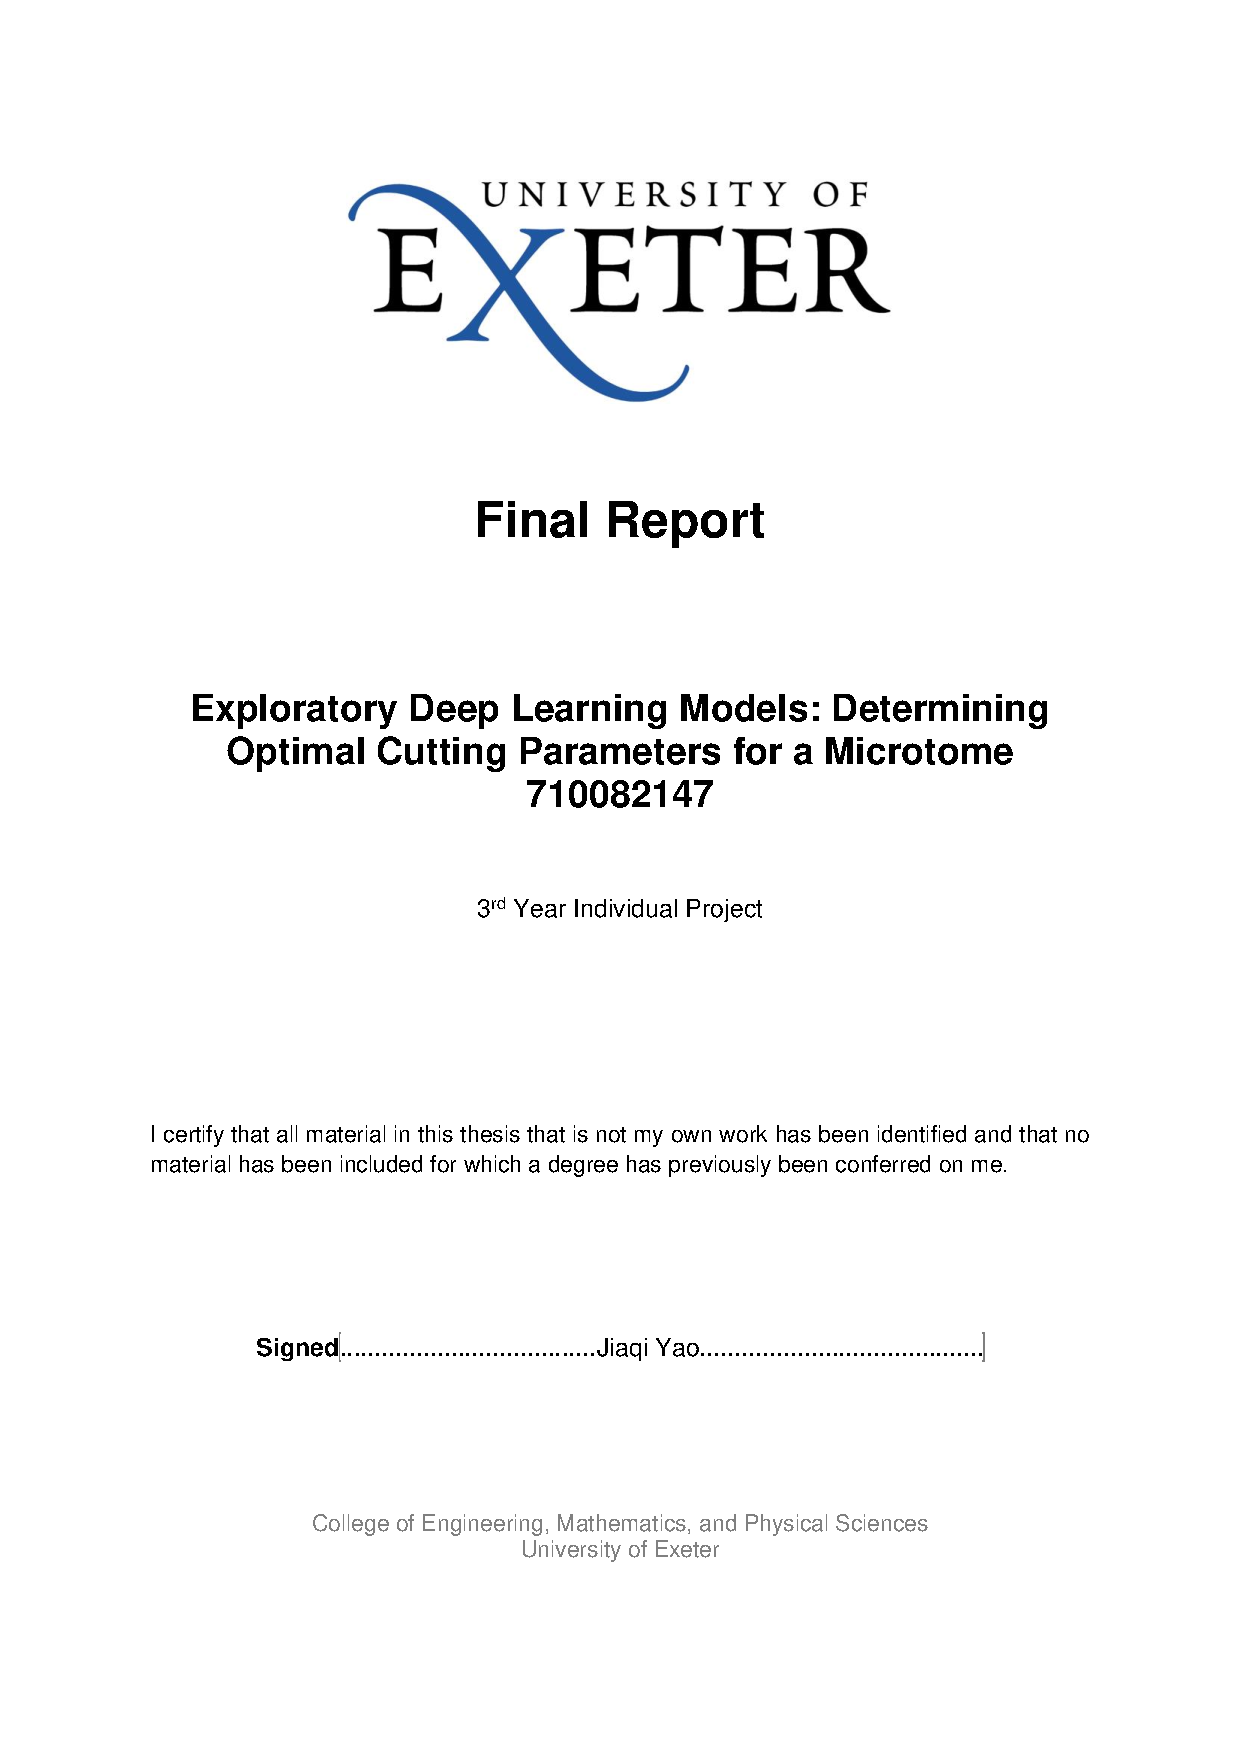
\includepdf[pages=1-3]{封面.pdf}


%目录(前三行为目录格式调整)
%\cftsetindents{section}{0em}{2em}
%\cftsetindents{subsection}{2em}{3em}
%\cftsetindents{subsubsection}{4em}{4em}
\newpage
{
	\fontspec{Times New Roman}
	\tableofcontents
}
\newpage


%
%以下部分为正文内容
\pagenumbering{arabic}
\section{Introduction and background}
\label{sec:introduction}


\subsection{Introduction}

\subsubsection{Project Overview}

This project addresses the critical task of optimizing the cutting parameters of a biological tissue slicer, an essential instrument in biomedical research and clinical diagnostics. The aim is to enhance the precision and efficiency of tissue sample preparation by identifying the optimal slicing conditions. Through the collection of tissue samples under various cutting parameters and subsequent artificial image classification, this study employs deep learning techniques to analyze and predict the most effective slicing parameters. This endeavor not only promises to improve the quality of tissue samples for microscopic examination but also to streamline the workflow in laboratories, thereby contributing to the advancement of biological and medical sciences.
% 这个项目解决了生物组织切片仪的关键任务,这是生物医学研究和临床诊断中的一个重要仪器。其目标是通过确定最佳切片条件来提高组织样本制备的精确性和效率。通过收集在不同切割参数下的组织样本,并进行人工图像分类,本研究采用深度学习技术来分析和预测最有效的切片参数。这个努力不仅有望改善显微镜检查的组织样本质量,还有望简化实验室的工作流程,从而促进生物和医学科学的进步。
\subsubsection{Objectives}

\begin{enumerate}
    \item Collect a comprehensive dataset of tissue samples sliced under different parameters.
    \item Employ artificial image classification to categorize the quality and characteristics of these samples.
    \item Develop and train a deep learning model capable of assessing tissue sample quality.
    \item Use the model's insights to determine the optimal cutting parameters for the tissue slicer.
    \item Validate the model's predictions through empirical testing and refinement.
\end{enumerate}

% \item 收集在不同参数下切割的组织样本的全面数据集。
% \item 使用人工图像分类来对这些样本的质量和特征进行分类。
% \item 开发和训练一个能够评估组织样本质量的深度学习模型。
% \item 利用模型的见解来确定组织切片仪的最佳切割参数。
% \item 通过实证测试和改进来验证模型的预测结果。
% \end{enumerate}

\subsubsection{Structure of the Report}

This project is organized into the following chapters, each designed to systematically explore the research background, methodologies, experimental work, results presentation, discussions and conclusions, as well as considerations for project management, sustainability, and health and safety:

\textbf{Introduction and Background} - This chapter outlines the project's objectives, goals, and structural arrangement. It provides a brief introduction to the motivation and necessity for the research, along with the technical protocols and specifications adopted.

\textbf{Literature Review} - An in-depth discussion on the use of biological tissue slicers, image classification, and deep learning in the preparation of biological samples. This section positions the current study within the context of existing research.

\textbf{Methodology and Theory} - Detailed descriptions of the experimental methods, theoretical frameworks, and the specific plans for data collection and processing are presented here.

\textbf{Experimental Work/Analytical Investigation/Design} - Describes the detailed steps of experimental design, implementation, and analytical investigation. It elaborates on the strategies and methods adopted to achieve the project's objectives.

\textbf{Presentation of Experimental or Analytical Results/Descriptions of Final Constructed Product} - This chapter showcases the experimental data, analysis results, or the final design product, providing detailed accounts of the experimental or design outcomes.

\textbf{Discussion and Conclusions} - The results are analyzed, and their scientific significance and practical value are discussed. This chapter also offers the research conclusions and suggests potential directions for future studies.

\textbf{Project Management, Consideration of Sustainability and Health and Safety} - Discusses strategies for project management, sustainability issues, and health and safety measures to ensure the research work is conducted efficiently and safely.

\textbf{References} - Lists all the bibliographic materials cited, supporting the research and providing the basis for the study.
% 本项目分为以下几个章节,每个章节都旨在系统地探索研究背景、方法论、实验工作、结果展示、讨论和结论,以及项目管理、可持续性和健康安全方面的考虑:

% \textbf{引言和背景} - 本章概述了项目的目标、目标和结构安排。它简要介绍了研究的动机和必要性,以及采用的技术协议和规范。

% \textbf{文献综述} - 对生物组织切片、图像分类和深度学习在生物样本制备中的应用进行深入讨论。本节将当前研究定位于现有研究的背景下。

% \textbf{方法和理论} - 详细描述了实验方法、理论框架以及数据收集和处理的具体计划。

% \textbf{实验工作/分析调查/设计} - 描述了实验设计、实施和分析调查的详细步骤。详细阐述了实现项目目标所采用的策略和方法。

% \textbf{实验或分析结果展示/最终构建产品描述} - 本章展示了实验数据、分析结果或最终设计产品,详细描述了实验或设计结果。

% \textbf{讨论和结论} - 对结果进行分析,讨论其科学意义和实际价值。本章还提供研究结论,并提出未来研究的潜在方向。

% \textbf{项目管理、可持续性和健康安全考虑} - 讨论项目管理策略、可持续性问题和健康安全措施,以确保研究工作的高效和安全进行。

% \textbf{参考文献} - 列出所有引用的文献资料,支持研究并为研究提供基础。

\subsubsection{Assumptions and Technical Specifications}

The project is based on several key assumptions and technical protocols, which are:

\begin{enumerate}
    \item The consistency in tissue sample properties across different batches.
    \item The reliability and precision of the biological tissue slicer and imaging equipment.
    \item The adequacy of the deep learning model in interpreting complex biological image data.
\end{enumerate}
Technical specifications regarding the tissue slicer settings, image classification criteria, and deep learning architecture are detailed in \textbf{Methodology and Theory}.
% 该项目基于几个关键假设和技术协议,包括:

% \begin{enumerate}
%     \item 不同批次之间组织样本性质的一致性。
%     \item 生物组织切片仪和成像设备的可靠性和精确性。
%     \item 深度学习模型在解释复杂生物图像数据方面的充分性。
% \end{enumerate}
% 有关组织切片仪设置、图像分类标准和深度学习架构的技术规格详见方法和理论。

\subsection{Background}

\subsubsection{Importance of Tissue Sample Quality}

High-quality tissue samples are pivotal for accurate diagnosis and research. The quality of a tissue sample can significantly affect the results of histological analysis, making the optimization of slicing parameters a crucial endeavor.

\subsubsection{Advancements in Image Classification and Deep Learning}

Recent advancements in image classification and deep learning have opened new avenues for automating and enhancing the analysis of biological samples. By leveraging these technologies, it is possible to achieve greater accuracy and efficiency in identifying optimal tissue slicing parameters.

\subsubsection{Gap in Current Research}

While there have been significant strides in both biological sample preparation and computational analysis, a gap remains in integrating these approaches to optimize tissue slicing parameters. This project aims to bridge this gap by developing a predictive model that can guide the adjustment of slicing conditions for optimal outcomes.

% \subsection{背景}

% \subsubsection{组织样本质量的重要性}

% 高质量的组织样本对于准确的诊断和研究至关重要。组织样本的质量可以显著影响组织学分析的结果,因此优化切片参数是一项关键的工作。

% \subsubsection{图像分类和深度学习的进展}

% 图像分类和深度学习的最新进展为自动化和增强生物样本分析开辟了新的途径。通过利用这些技术,可以在识别最佳组织切片参数方面实现更高的准确性和效率。

% \subsubsection{当前研究中的差距}

% 尽管在生物样本制备和计算分析方面取得了重大进展,但在整合这些方法以优化组织切片参数方面仍存在差距。本项目旨在通过开发一个预测模型来填补这一差距,该模型可以指导调整切片条件以获得最佳结果。

\section{Literature review}

\subsection{Technical background to tissue slicing and image acquisition}

%组织切片和图像获取的技术背景   这里写切片机和显微镜的技术参数和采集手册及方法

\subsection{Image Classification for Tissue Analysis}

%用于组织分析的图像分类   这里写图像分类的技术背景和方法


\subsection{Deep Learning in Biomedical Applications}

%深度学习在生物医学应用中的应用   这里写深度学习的技术背景和方法

\subsection{Integration of Deep Learning for Optimizing Tissue Slicing Parameters}

%整合深度学习以优化组织切片参数   这里写深度学习在优化切片参数中的应用


\FloatBarrier % Now figures cannot float above section title




\section{Literature review}


这篇文献综述探讨了生物组织切片中技术的融合,特别关注图像分类和深度学习在优化切片参数方面的应用。它旨在突出重要的进展,确定当前方法学中存在的差距,并为拟议的项目奠定基础。

\subsection{切片机与显微镜}

近年来,自动切片机的出现显著简化了切片过程,并提高了切片的质量。

Zimmermann在文章"Improved reproducibility in preparing precision-cut liver tissue slices"中,主张使用新的Leica振动刀来提高大鼠、小鼠和人体组织切片的精度和重复性 \cite{LR.1}。

在这个实验中,我们使用Epredia提供的HM355S切片机进行切片。这台机器是生物组织切片研究的流行设备,许多实验和论文都使用了这台设备进行切片。

Elzbieta Klimuszko使用HM355S切片机切割牙齿,以研究牙釉质中的钙和镁含量 \cite{LR.2}。

Andelko Hrzenjak也使用HM355S切片机切割病理性子宫内膜组织,以研究子宫内膜癌发展的机制 \cite{LR.3}。

同样,显微镜的选择也至关重要。在这个实验中,我们使用Keyence的VHX7000显微镜进行图像采集。它能够捕获生物组织切片的图像(例如,小鼠前列腺细胞 \cite{LR.4}),以及无机材料(如陶瓷 \cite{LR.5},玻璃 \cite{LR.6})。

实验将使用HM355s切片机和VHX7000显微镜进行切片和图像采集。这种设置确保了设备选择和技术应用的最佳配合,以提高组织切片过程的精度和效率,支持研究项目的总体目标。

% \subsection{深度学习的原理}










\subsection{关于切片组织的深度学习}

在生物医学领域,深度学习技术的应用已取得了显著的进步。深度学习模型在图像分类、对象检测和分割等任务中表现出色,为生物医学实验室的研究和诊断提供了强大的工具。

Lorena Guachi-Guachi 提出了一种利用 CNN 网络识别和精炼组织切片的方法。这种方法代表了深度学习的创新应用,可以提高组织准备和分析的精度 \cite{LR.7}。

在《生物医学纹理分析》一书中,Vincent Andrearczyk 介绍了一种专为纹理分析设计的 CNN 架构,与传统架构相比,这种架构显著提高了生物组织分类的准确性 \cite{LR.8}。这一发展展示了深度学习提高组织特性详细分析的潜力,这对于准确的诊断和研究至关重要。

Yan Xu 提出,从在大型自然图像数据库 ImageNet 上训练的 CNN 中提取的特征可以转移到组织的病理学图像上。这为实施转移学习提供了一种可行的方法,可以大大提高组织图像分类和分析的效率 \cite{LR.9}。

根据文献,深度学习技术在组织切片的图像分类和分析中有广阔的应用前景。通过利用深度学习模型,可以实现组织样本的有效识别和分类,为优化切片参数提供了强大的支持。

这一部分强调了深度学习对组织切片领域的变革性影响,预示着在组织学分析的准确性和实用性方面的显著改进。

\FloatBarrier % Now figures cannot float above section title

\section{Methodology and theory}
\label{sec:problem_description}

\subsection{计算机视觉-图像分割}

对于获取的图像数据,可以应用适当的图像预处理。在保持图像完整性和质量的前提下,可以实施某些处理以突出计算机识别的特征,并在一定程度上去除无关特征和噪声。这增强了后续深度学习模型的准确性。

图像分割是图像处理中的关键步骤,目的是将图像划分为几个有意义的区域以进行进一步的分析和处理。在关注生物组织产率的模型中,需要将生物切片分割为生物组织和石蜡区域,强调生物组织部分。

常见的图像分割算法包括边缘检测和阈值分割。

\subsubsection{边缘检测}
对于生物组织切片,质量的关键指标是切片边缘的清晰度。切片边缘的完整性和连续性可以反映样本是否存在质量问题。

有许多边缘检测的算法,如Sobel、Laplacian和Canny算子 \cite{3.1}。

\textbf{Sobel算子}是一种一阶差分算子,可以用来检测图像边缘 \cite{补充1}。假设有一个一维图像$f(x)$,其强度与像素坐标$x$的关系可以如图1所示。在\autoref{fig:original_function}中可以观察到,斜率在x=2.2附近最大,表明在这个点附近图像强度有突然的变化(存在边缘)。取其导数得到一阶导数$f'(x)$,如\autoref{fig:first_derivative}所示,其中导数的绝对值最大。Sobel算子利用这个特性来检测边缘。

\begin{figure}[htbp]
    \centering
    \begin{minipage}[b]{0.32\textwidth}
        \centering
        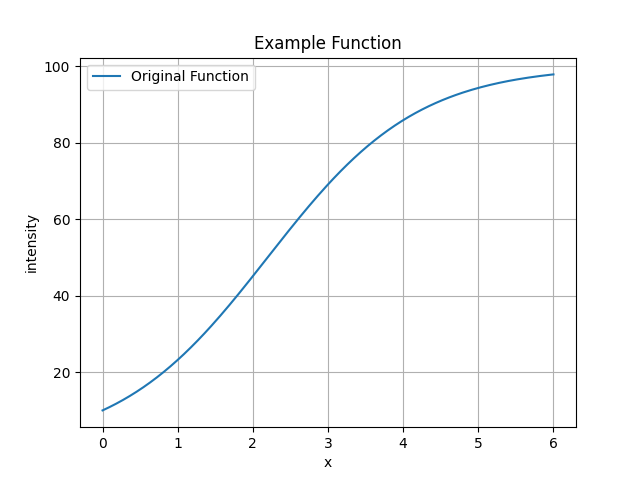
\includegraphics[width=\textwidth]{./fig/original_function.png}
        \caption{f(x)}
        \label{fig:original_function}
    \end{minipage}
    \begin{minipage}[b]{0.32\textwidth}
        \centering
        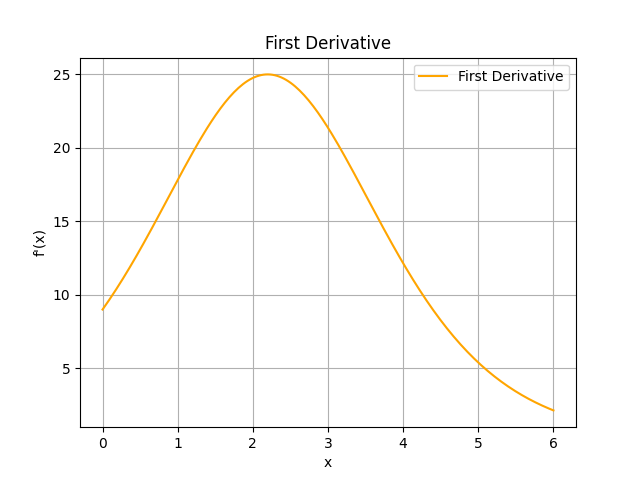
\includegraphics[width=\textwidth]{./fig/first_derivative.png}
        \caption{f'(x)}
        \label{fig:first_derivative}
    \end{minipage}
    \begin{minipage}[b]{0.32\textwidth}
        \centering
        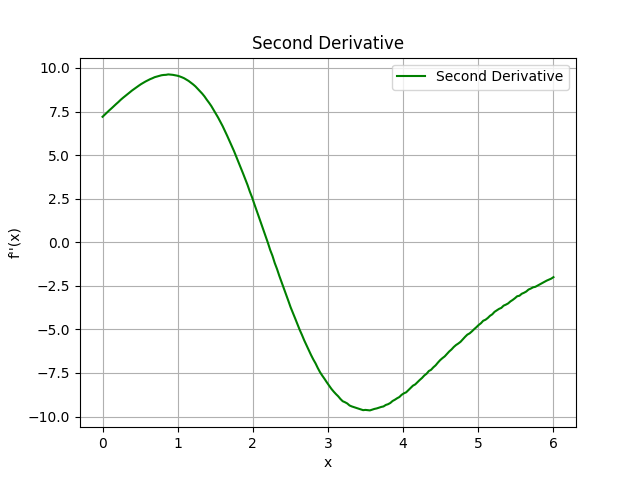
\includegraphics[width=\textwidth]{./fig/second_derivative.png}
        \caption{f''(x)}
        \label{fig:second_derivative}
    \end{minipage}
\end{figure}

\textbf{Laplacian算子}是一种二阶微分算子,其对图像的边缘检测效果较好。它是对sobel算子再进行一次求导得出。在2D图像中,Laplacian算子的定义如下:
\begin{equation}
    \nabla^2 f = \frac{\partial^2 f}{\partial x^2} + \frac{\partial^2 f}{\partial y^2}
\end{equation}
如上图所示,对一阶导数再次求导得到二阶导数$f''(x)$,如\autoref{fig:second_derivative}所示,可以看到在x=2.2左右,二阶导数为0,即说明当laplacian算子$\nabla^2 f$的值为0时,说明图像强度存在突变,即存在边缘。

\textbf{Canny算子}是一种多阶微分算子,他在sobel算子计算后的基础上加入了对噪声的抑制。他由John F. Canny于1986年提出\cite{3.2}.简而言之,其在sobel算子计算后,通过非极大值抑制,滞后阈值等步骤,设置了阈值,排除图像中的假边缘,得到了更加准确的边缘检测结果。

在Experimental work/analytical investigation/ design这一章节中 将会对采集到的图像数据进行三种边缘检测算法的实验,对比其效果。

\subsubsection{阈值分割}

除了边缘检测,还有一种方法是阈值分割。阈值分割是将图像中的像素点分为两类,一类是大于阈值的像素点,另一类是小于阈值的像素点。这种方法适用于图像中的目标和背景的灰度差异较大的情况。

对于样品来说,一个很简单的方法就是将石蜡区域和生物组织区域(样品在制备是已染色)的颜色进行对比,然后通过阈值分割的方法将其分割开来。假定生物组织为黄色,石蜡为白色,那么可以通过设置一个阈值,将图像中的白色部分分割出来,那么剩下的就是生物组织部分。

此外,关于阈值分割还有更多的方法,比如下面就是一个基于Otsu方法的指纹提取算法。将其用在此处能够显著提高生物组织的分割效果。
Yue Yaru和Zhu Jialin 在 《Algorithm of fingerprint extraction and implementation based on OpenCV》一文中提出了一种基于OpenCV的指纹提取算法。该算法对Otsu方法进行了改进,特别是在光照不均匀、图像模糊的情况下能够实现准确、简单、运行时间短的指纹提取。\cite{3.3}

相关的对比和实验将在 Experimental work/analytical investigation/ design这一章节中进行。


\FloatBarrier






 
\section{Experimental work/analytical investigation/ design}

\subsection{采集数据}
要进行深度学习,所需要的第一步就是采集数据。在本实验中,我们使用了预先从生物实验室制备好的石蜡包埋好的组织切片(鱼的卵巢组织),将其放在HM355s自动切片机上依据切片机的使用手册,以不同的切削角度执行切片操作。记录切削数据。

%在这不要提三个点的鱼的肺泡组织,在后面作为模型二次验证和增强使用。

其中切片机(\autoref{fig:machine})的切片示意图(以牙齿为例) 如\autoref{fig:cutting_machine}所示

\begin{figure}[htbp]
    \centering
    \begin{minipage}{0.48\textwidth}
        \centering
        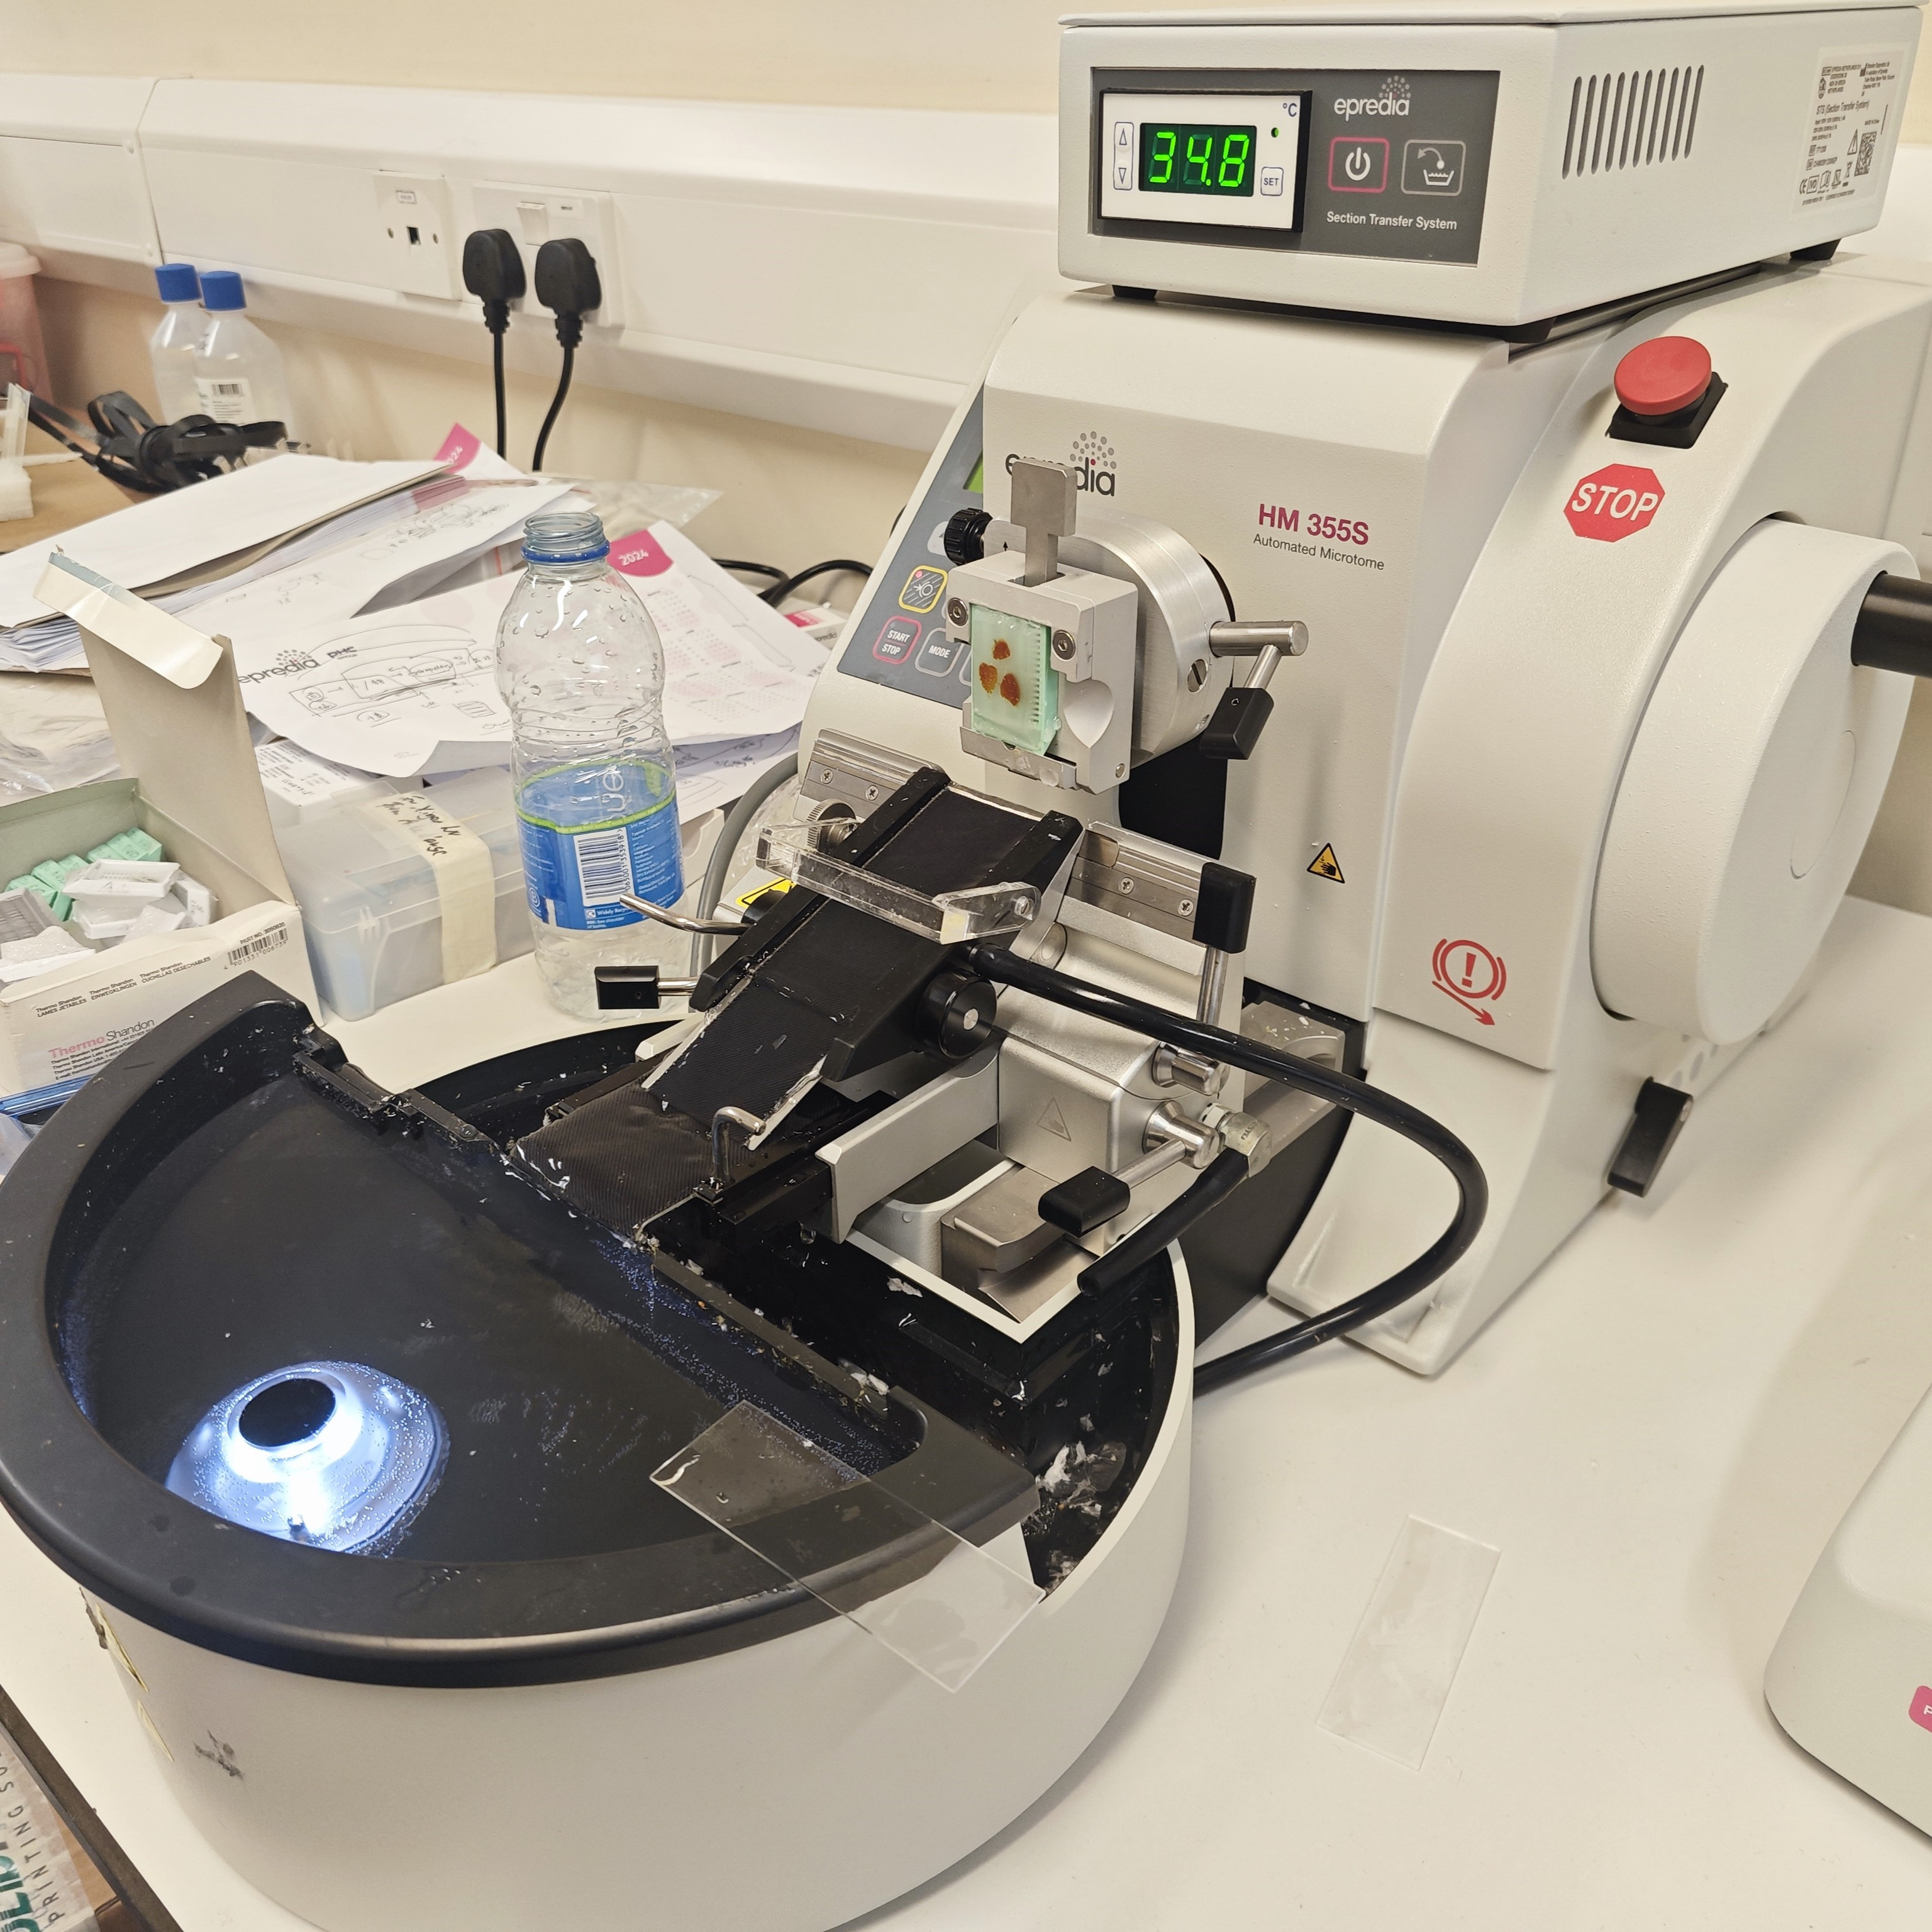
\includegraphics[width=\textwidth]{./fig/machine.jpg}
        \caption{切片机}
        \label{fig:machine}
    \end{minipage}
    \begin{minipage}{0.48\textwidth}
        \centering
        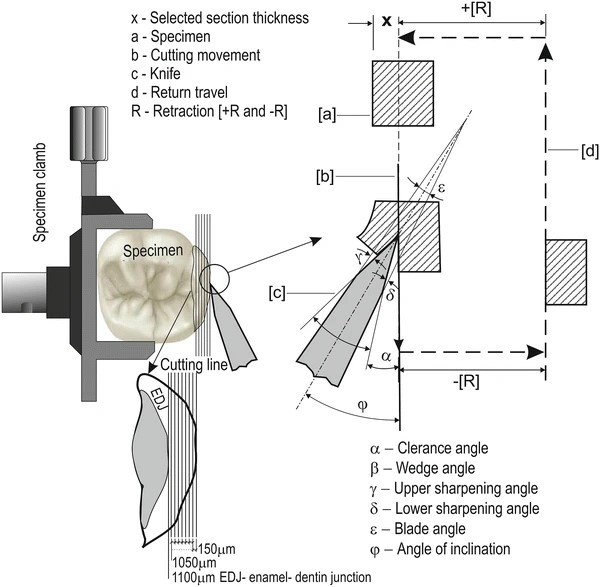
\includegraphics[width=\textwidth]{./fig/10266_2018_353_Fig1_HTML.jpg}
        \caption{切片机示意图}
        \label{fig:cutting_machine}
    \end{minipage}
\end{figure}
% https://link.springer.com/article/10.1007/s10266-018-0353-6


用于切片的生物组织(示例)如\autoref{label:sample}所示

在切削过程中,从切角为8度开始(如\autoref{fig:machine}中的angle of inclination),每次增加0.5度,直到切角为12度。切片机在切片过程中保持给进速度为25,厚度为1。

在切片完成之后,将切好的不同类型的组织切片放在载玻片上(如\autoref{fig:采集样本})所示,待其晾干后转移至VHX7000显微镜下,通过显微镜对每份样品进行拍照,获取到每份样品的电子图像数据(如\autoref{fig:显微镜})。

\begin{figure}[htbp]
    \centering
    \begin{minipage}{0.3\textwidth}
        \centering
        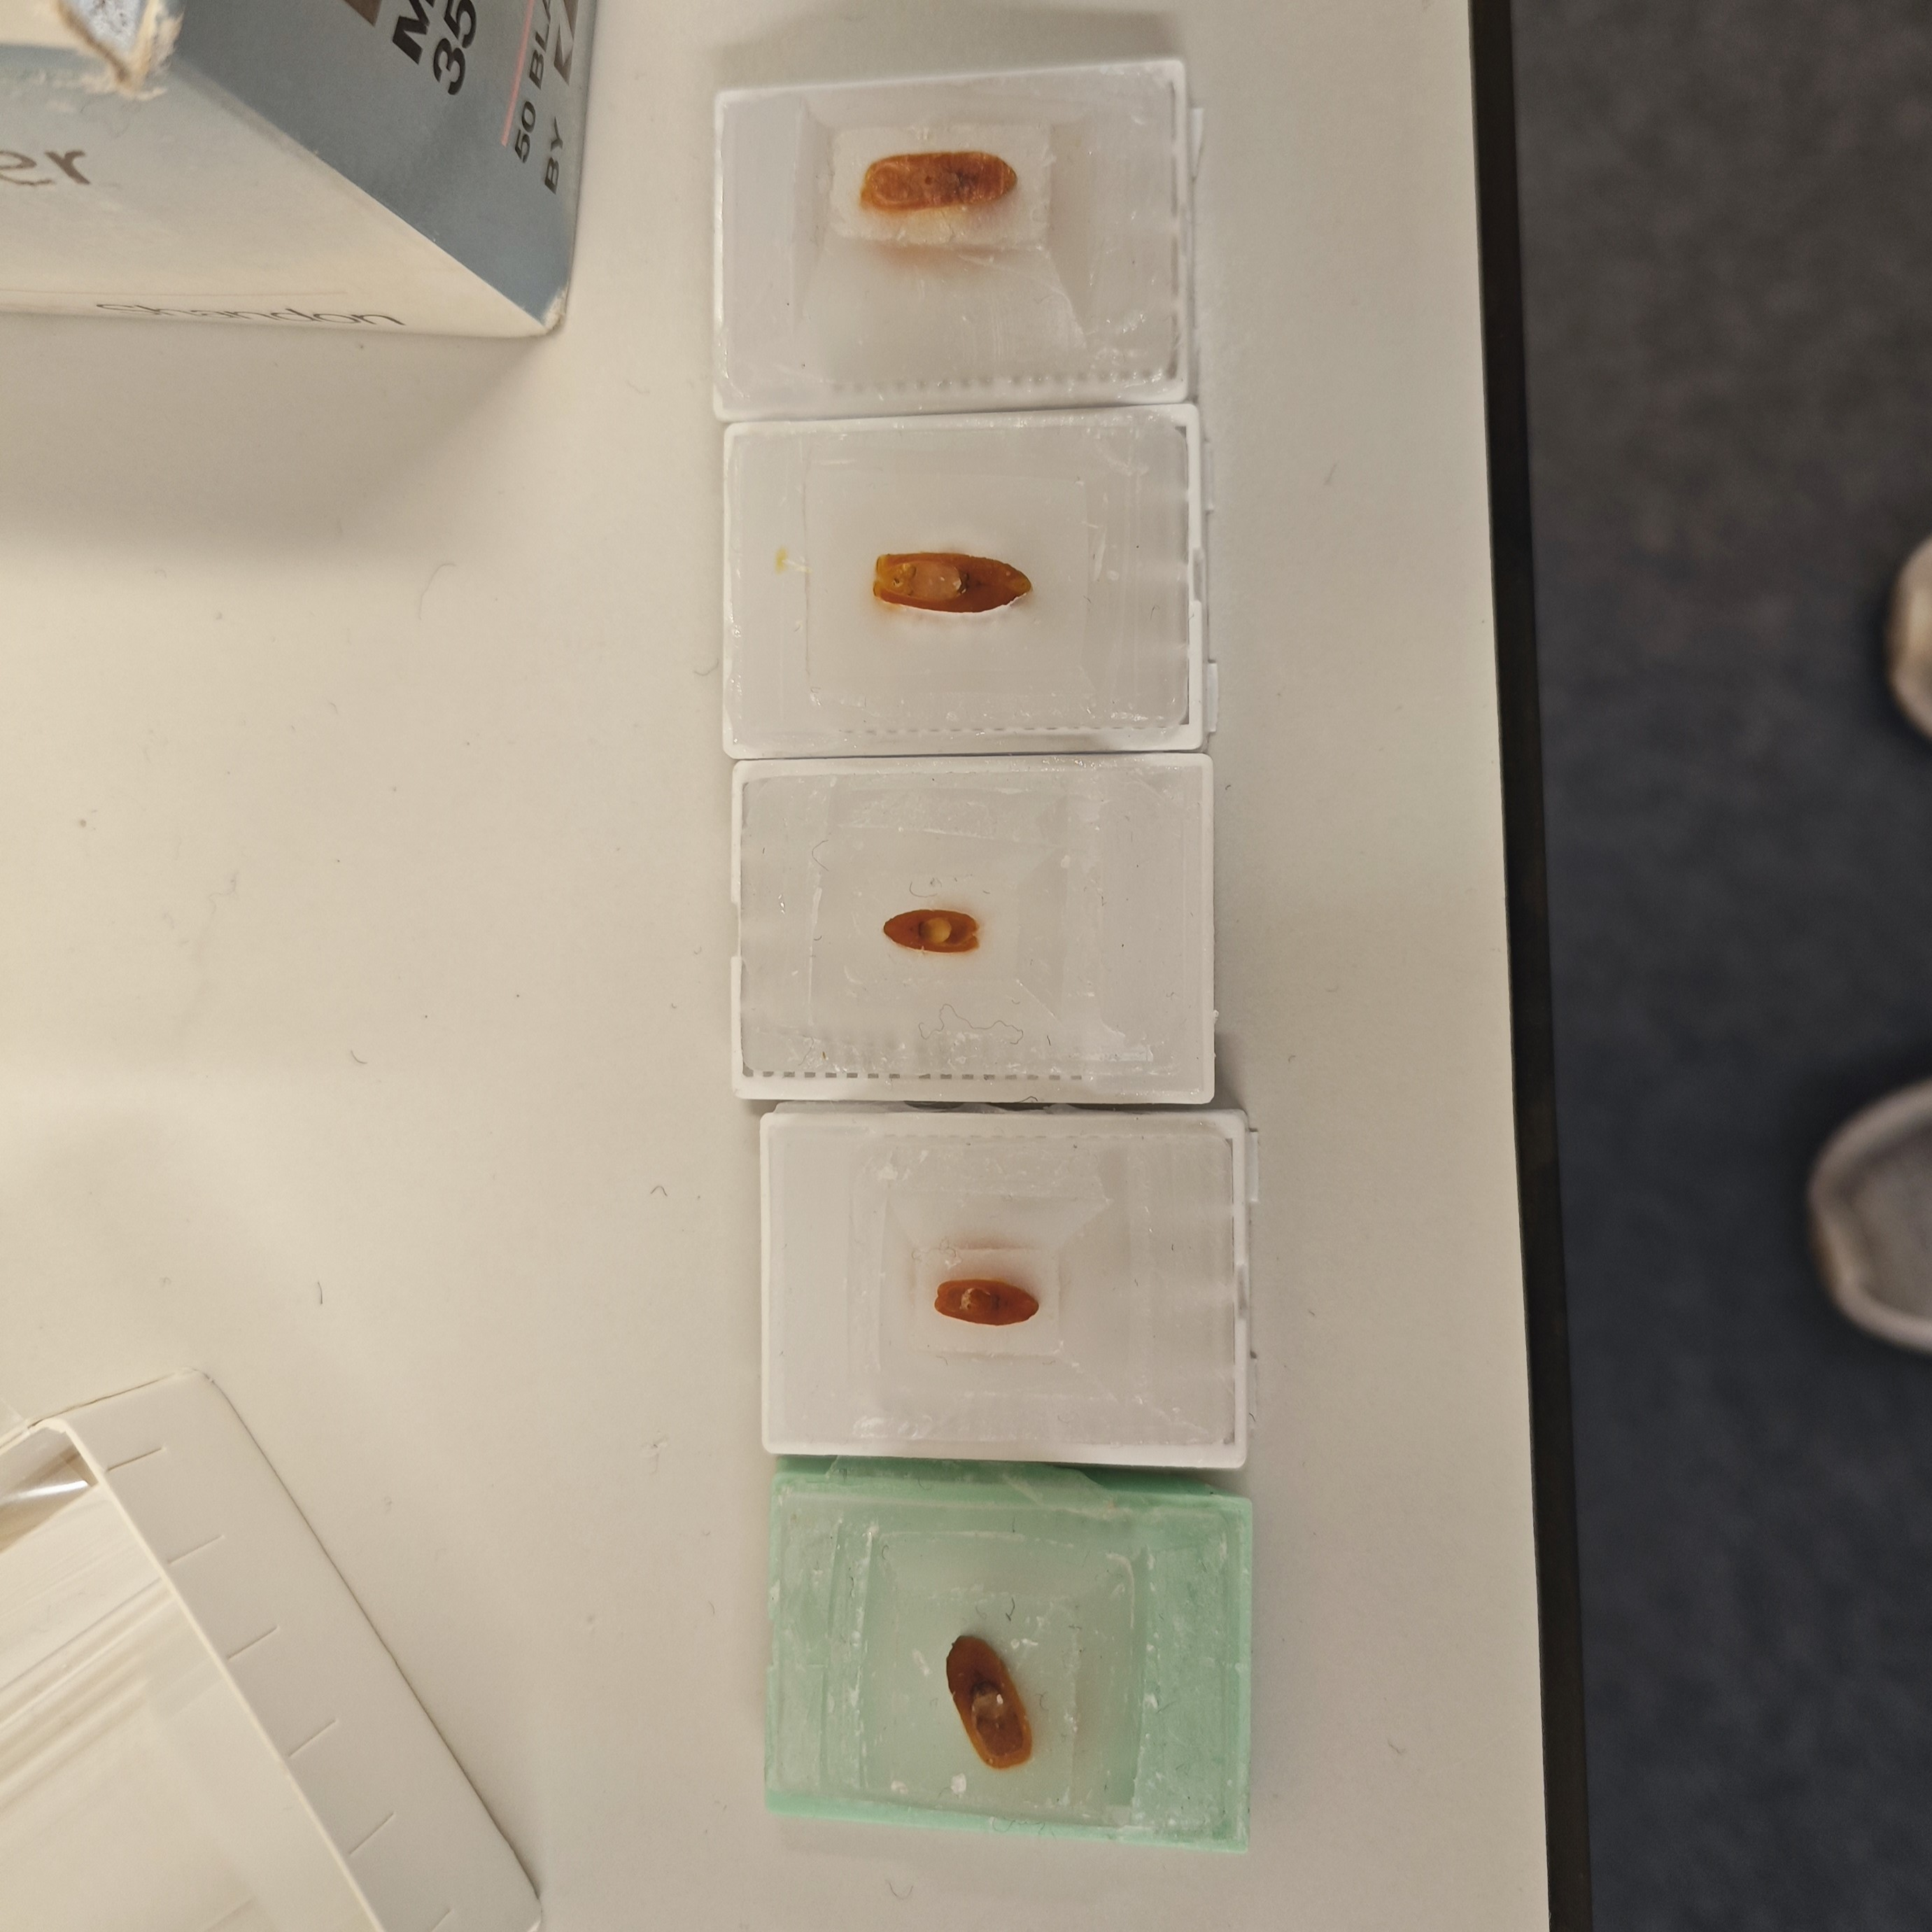
\includegraphics[width=\textwidth]{./fig/sample.jpg}
        \caption{生物组织切片}
        \label{label:sample}
    \end{minipage}
    \begin{minipage}{0.3\textwidth}
        \centering
        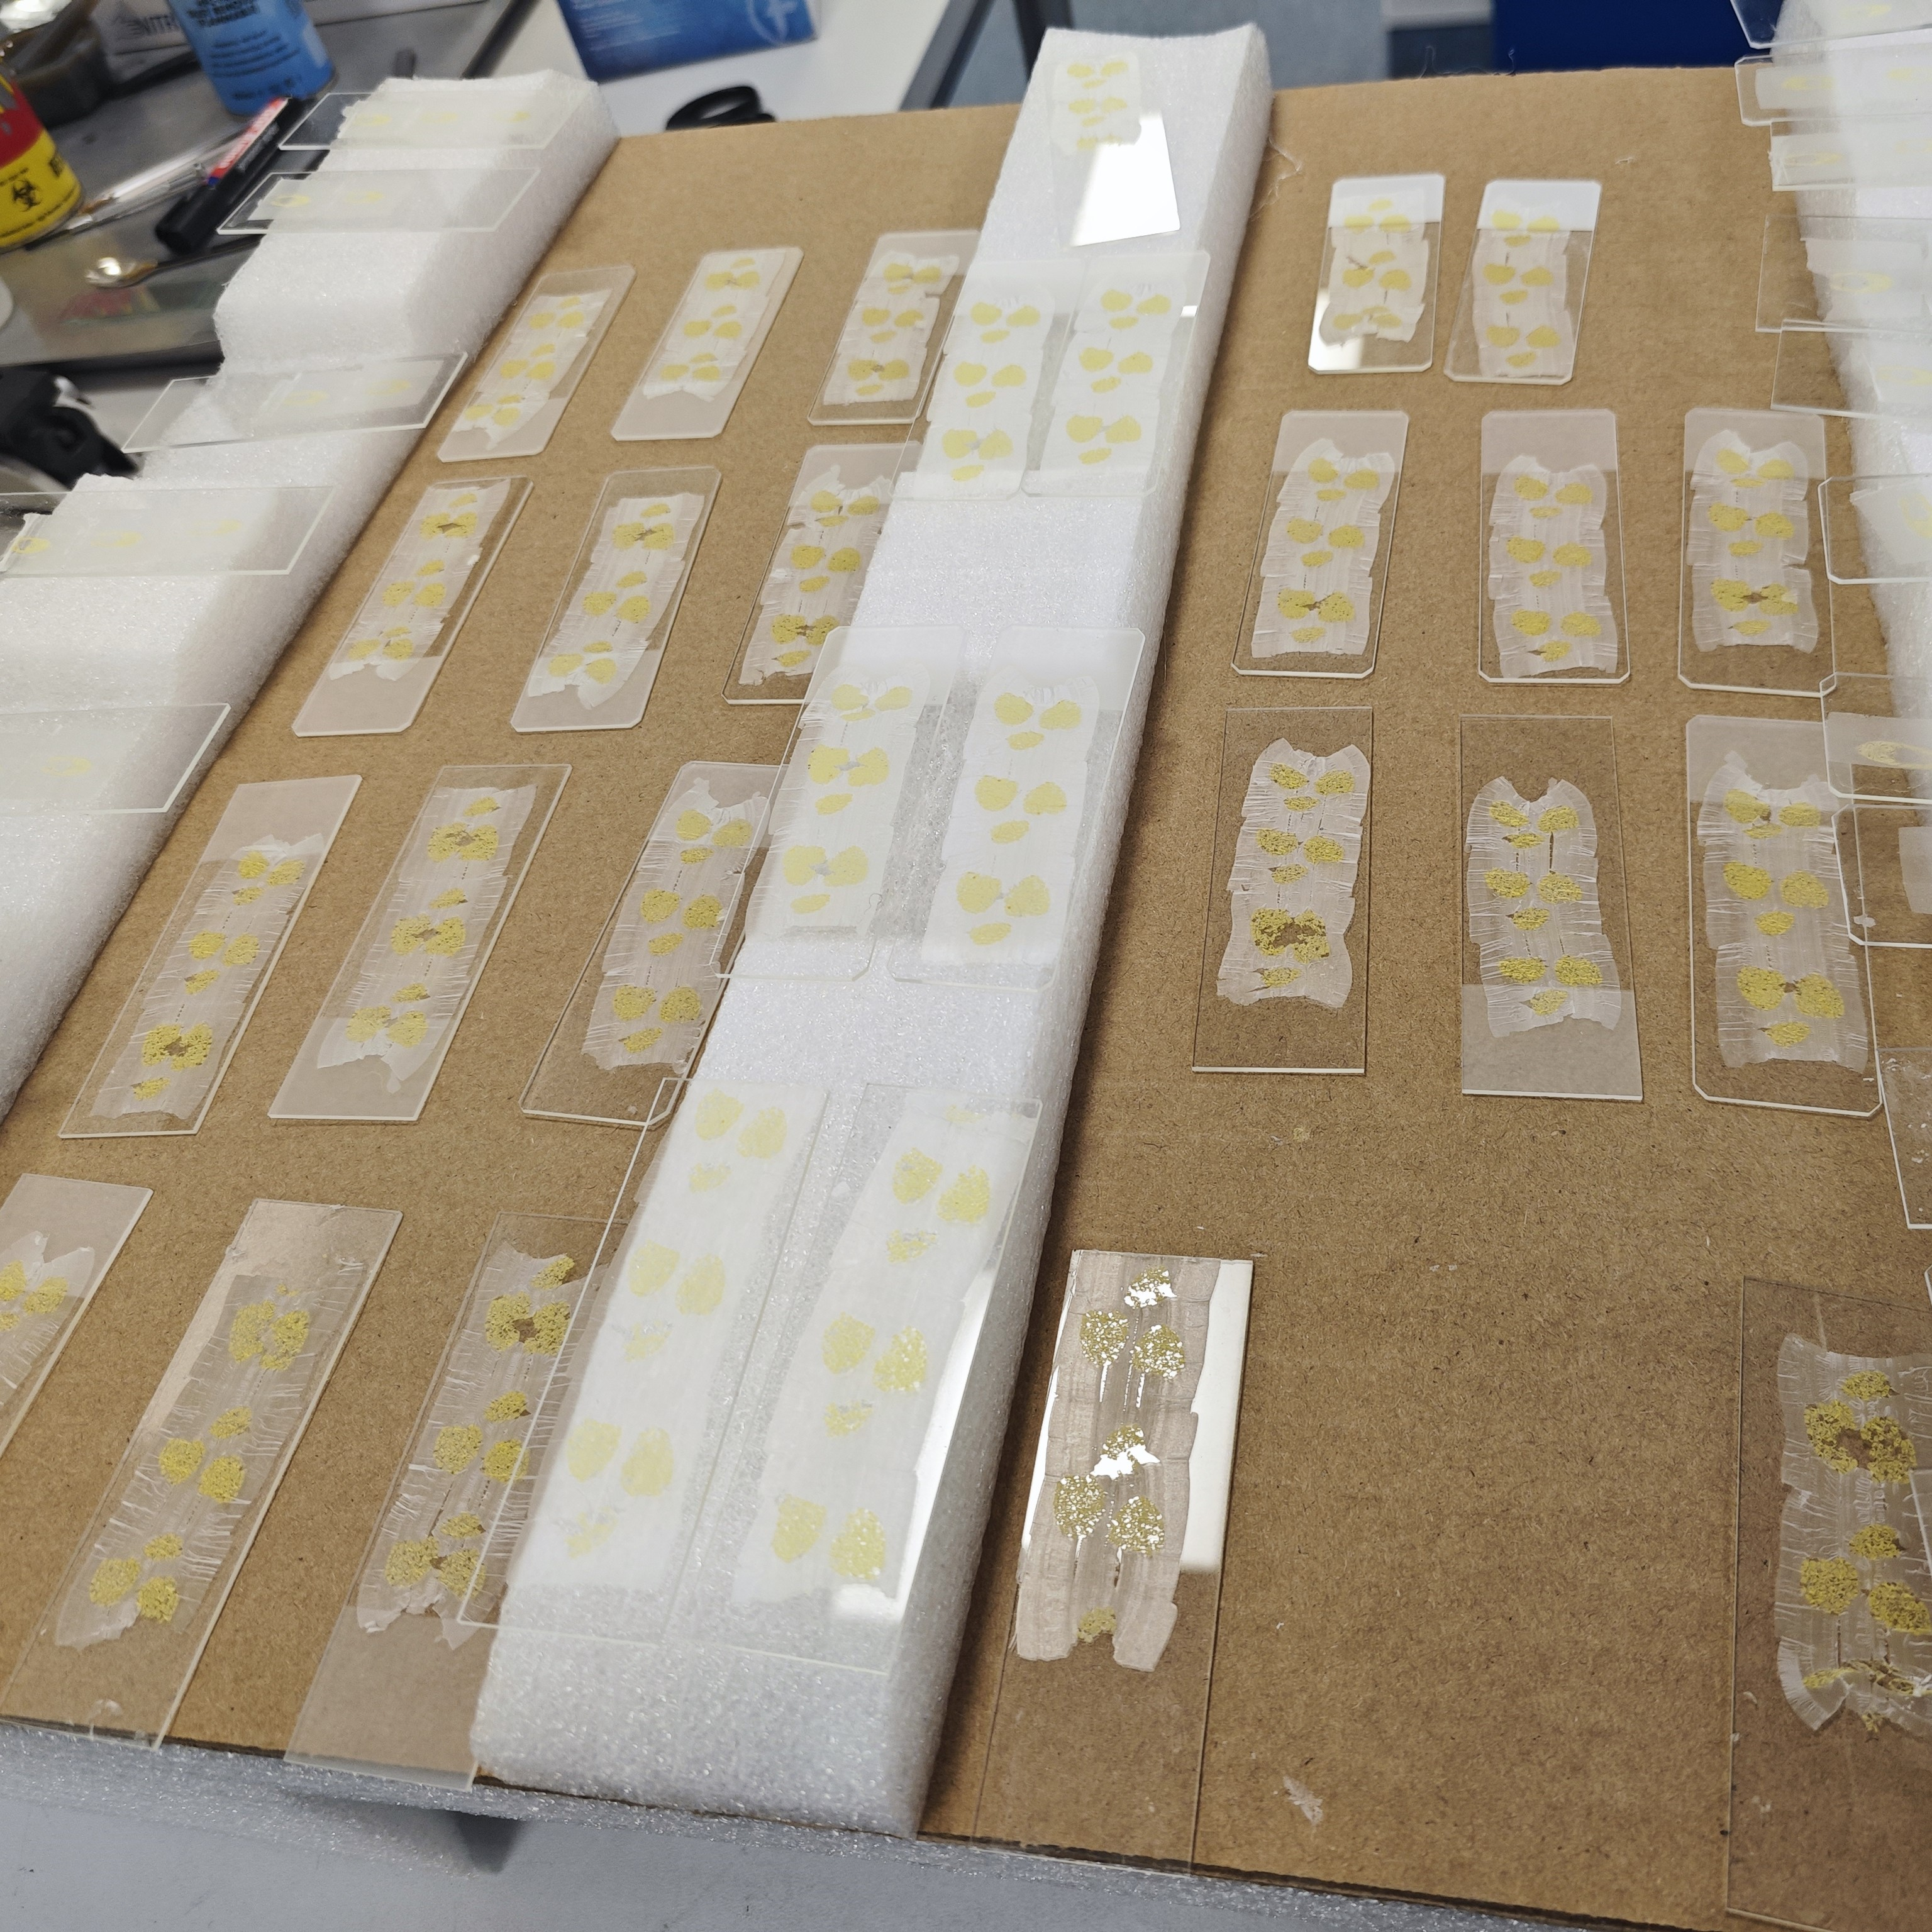
\includegraphics[width=\textwidth]{./fig/采集样本.jpg}
        \caption{采集样本}
        \label{fig:采集样本}
    \end{minipage}
    \begin{minipage}{0.35\textwidth}
        \centering
        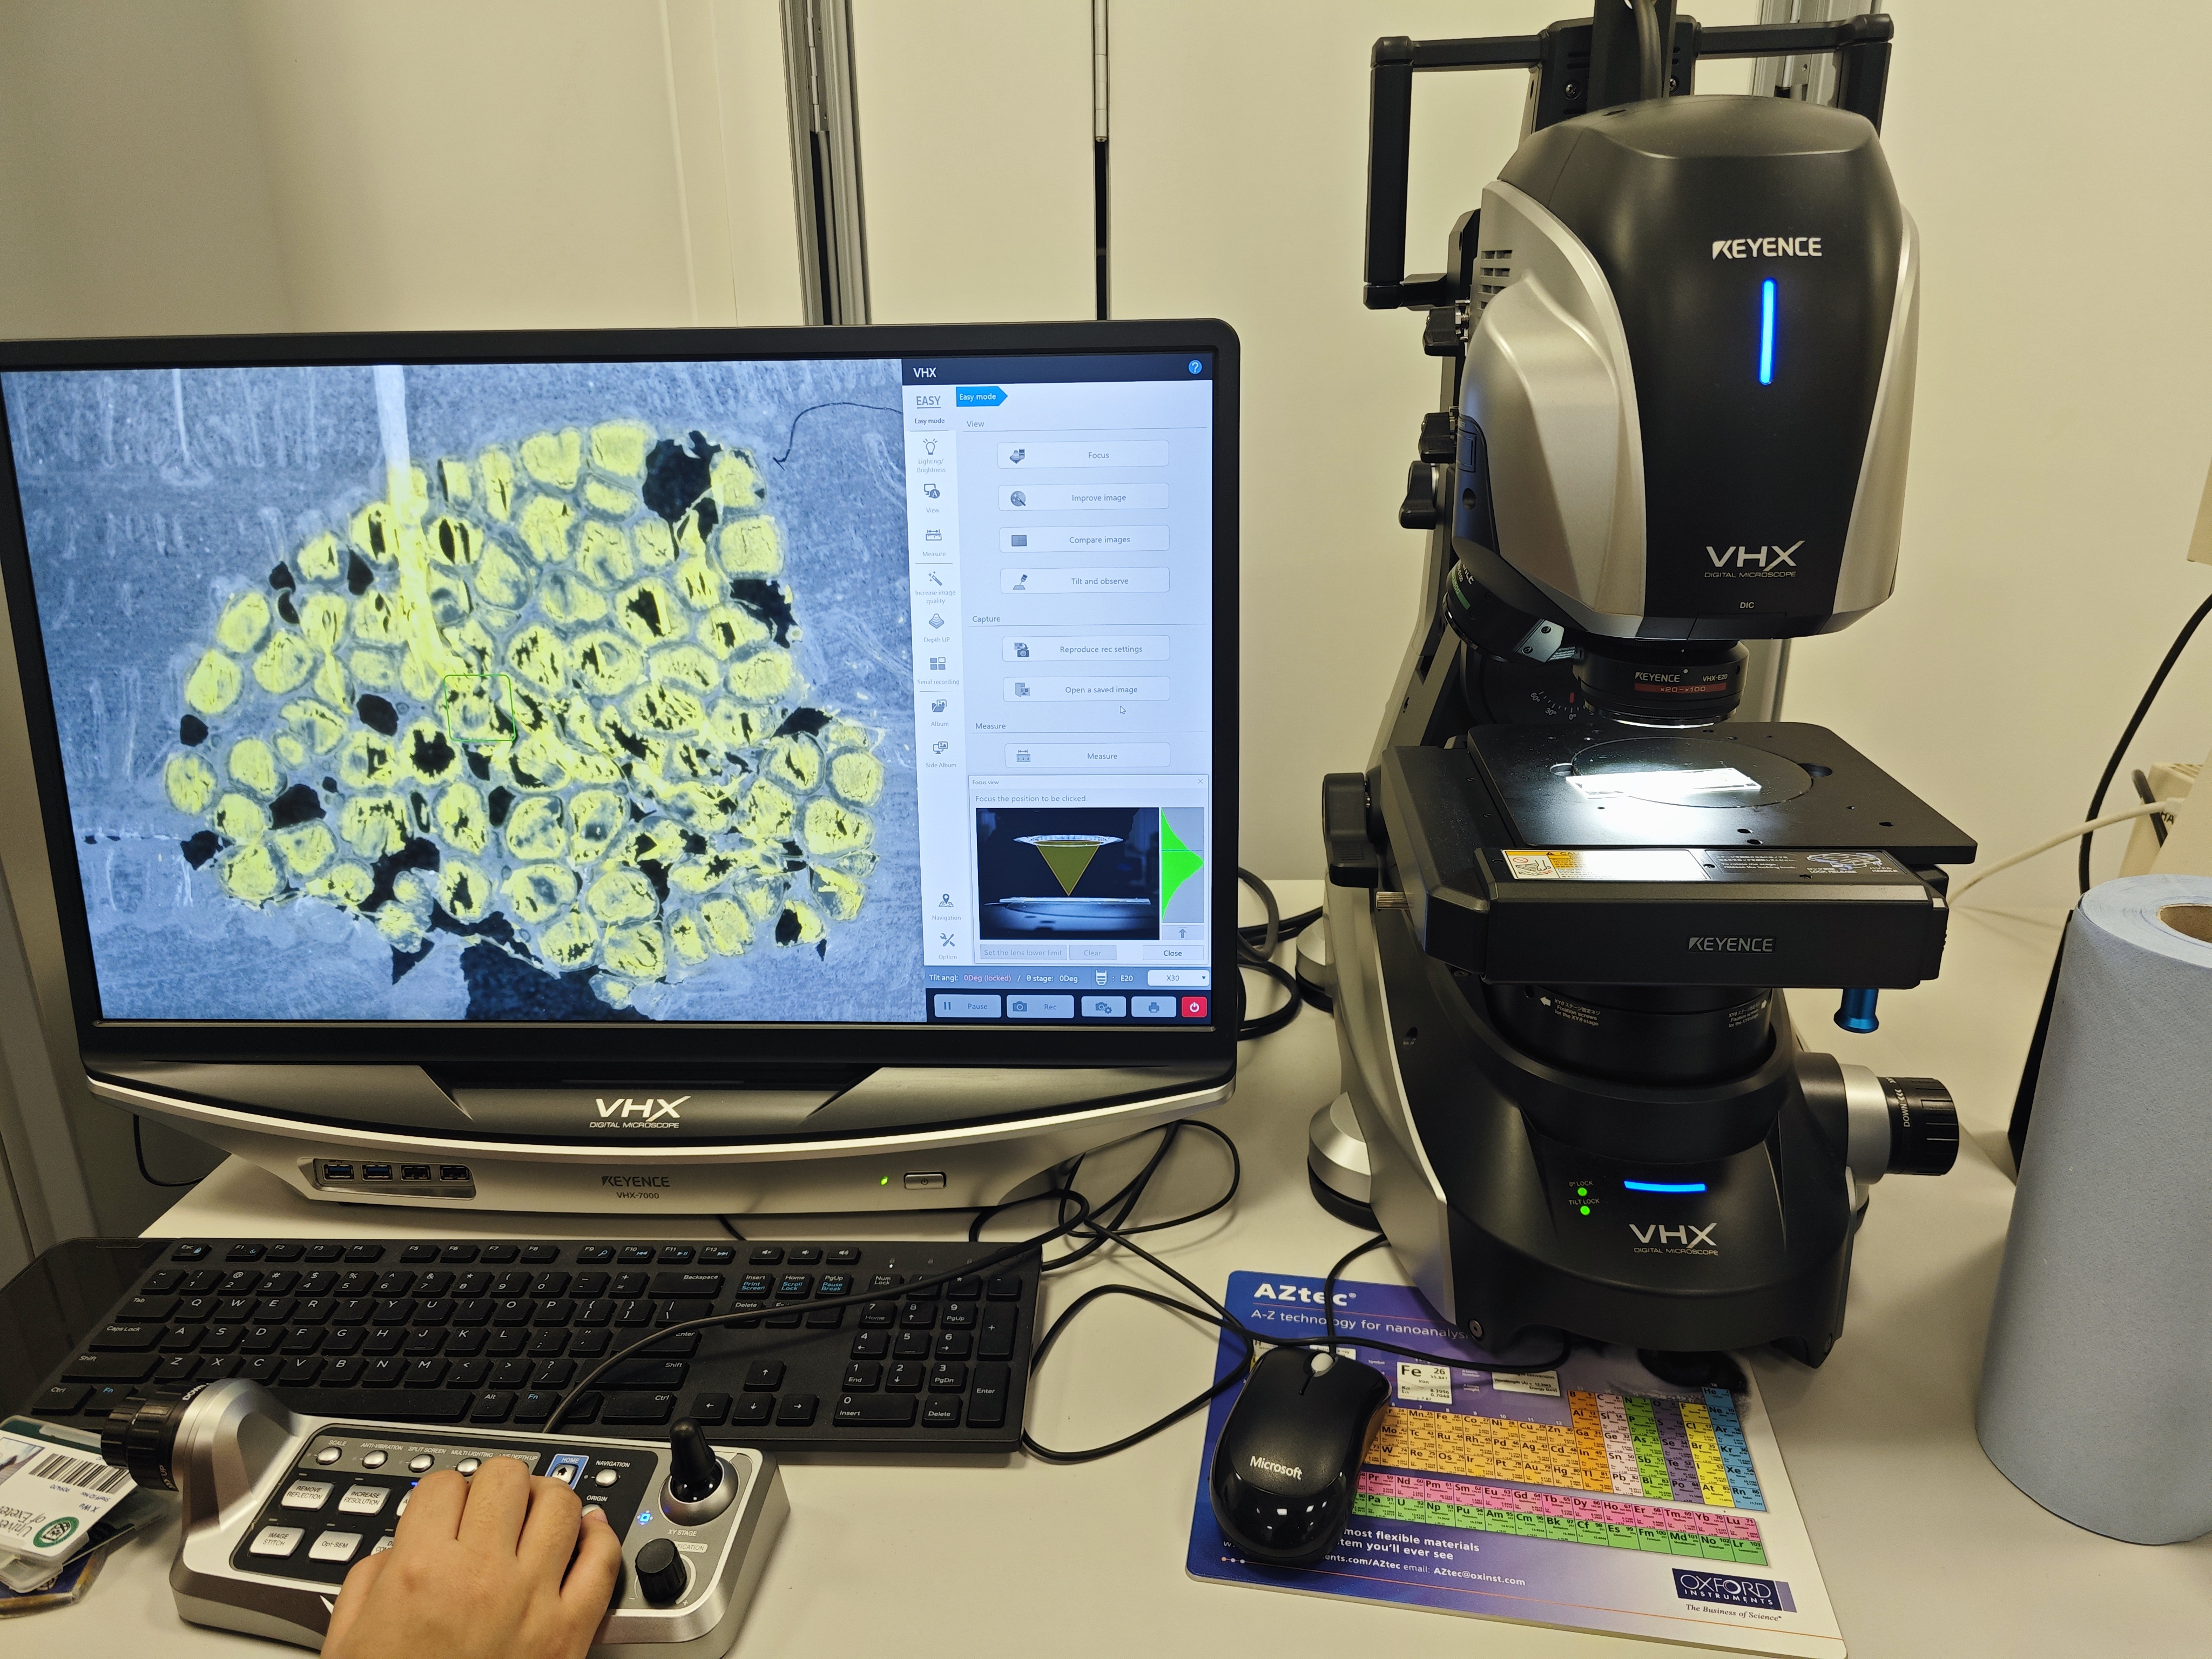
\includegraphics[width=\textwidth]{./fig/显微镜.jpg}
        \caption{显微镜}
        \label{fig:显微镜}
    \end{minipage}
\end{figure}

%图片需要后续更改为卵巢的

据此,一共得到9组数据,代表了从8到12每0.5度切角的数据。一共得到约为200张图片,每张图片的分辨率为2880*2160。其中一张(切角9.5度)如\autoref{fig:sample9.5}所示。

\begin{figure}
    \centering
    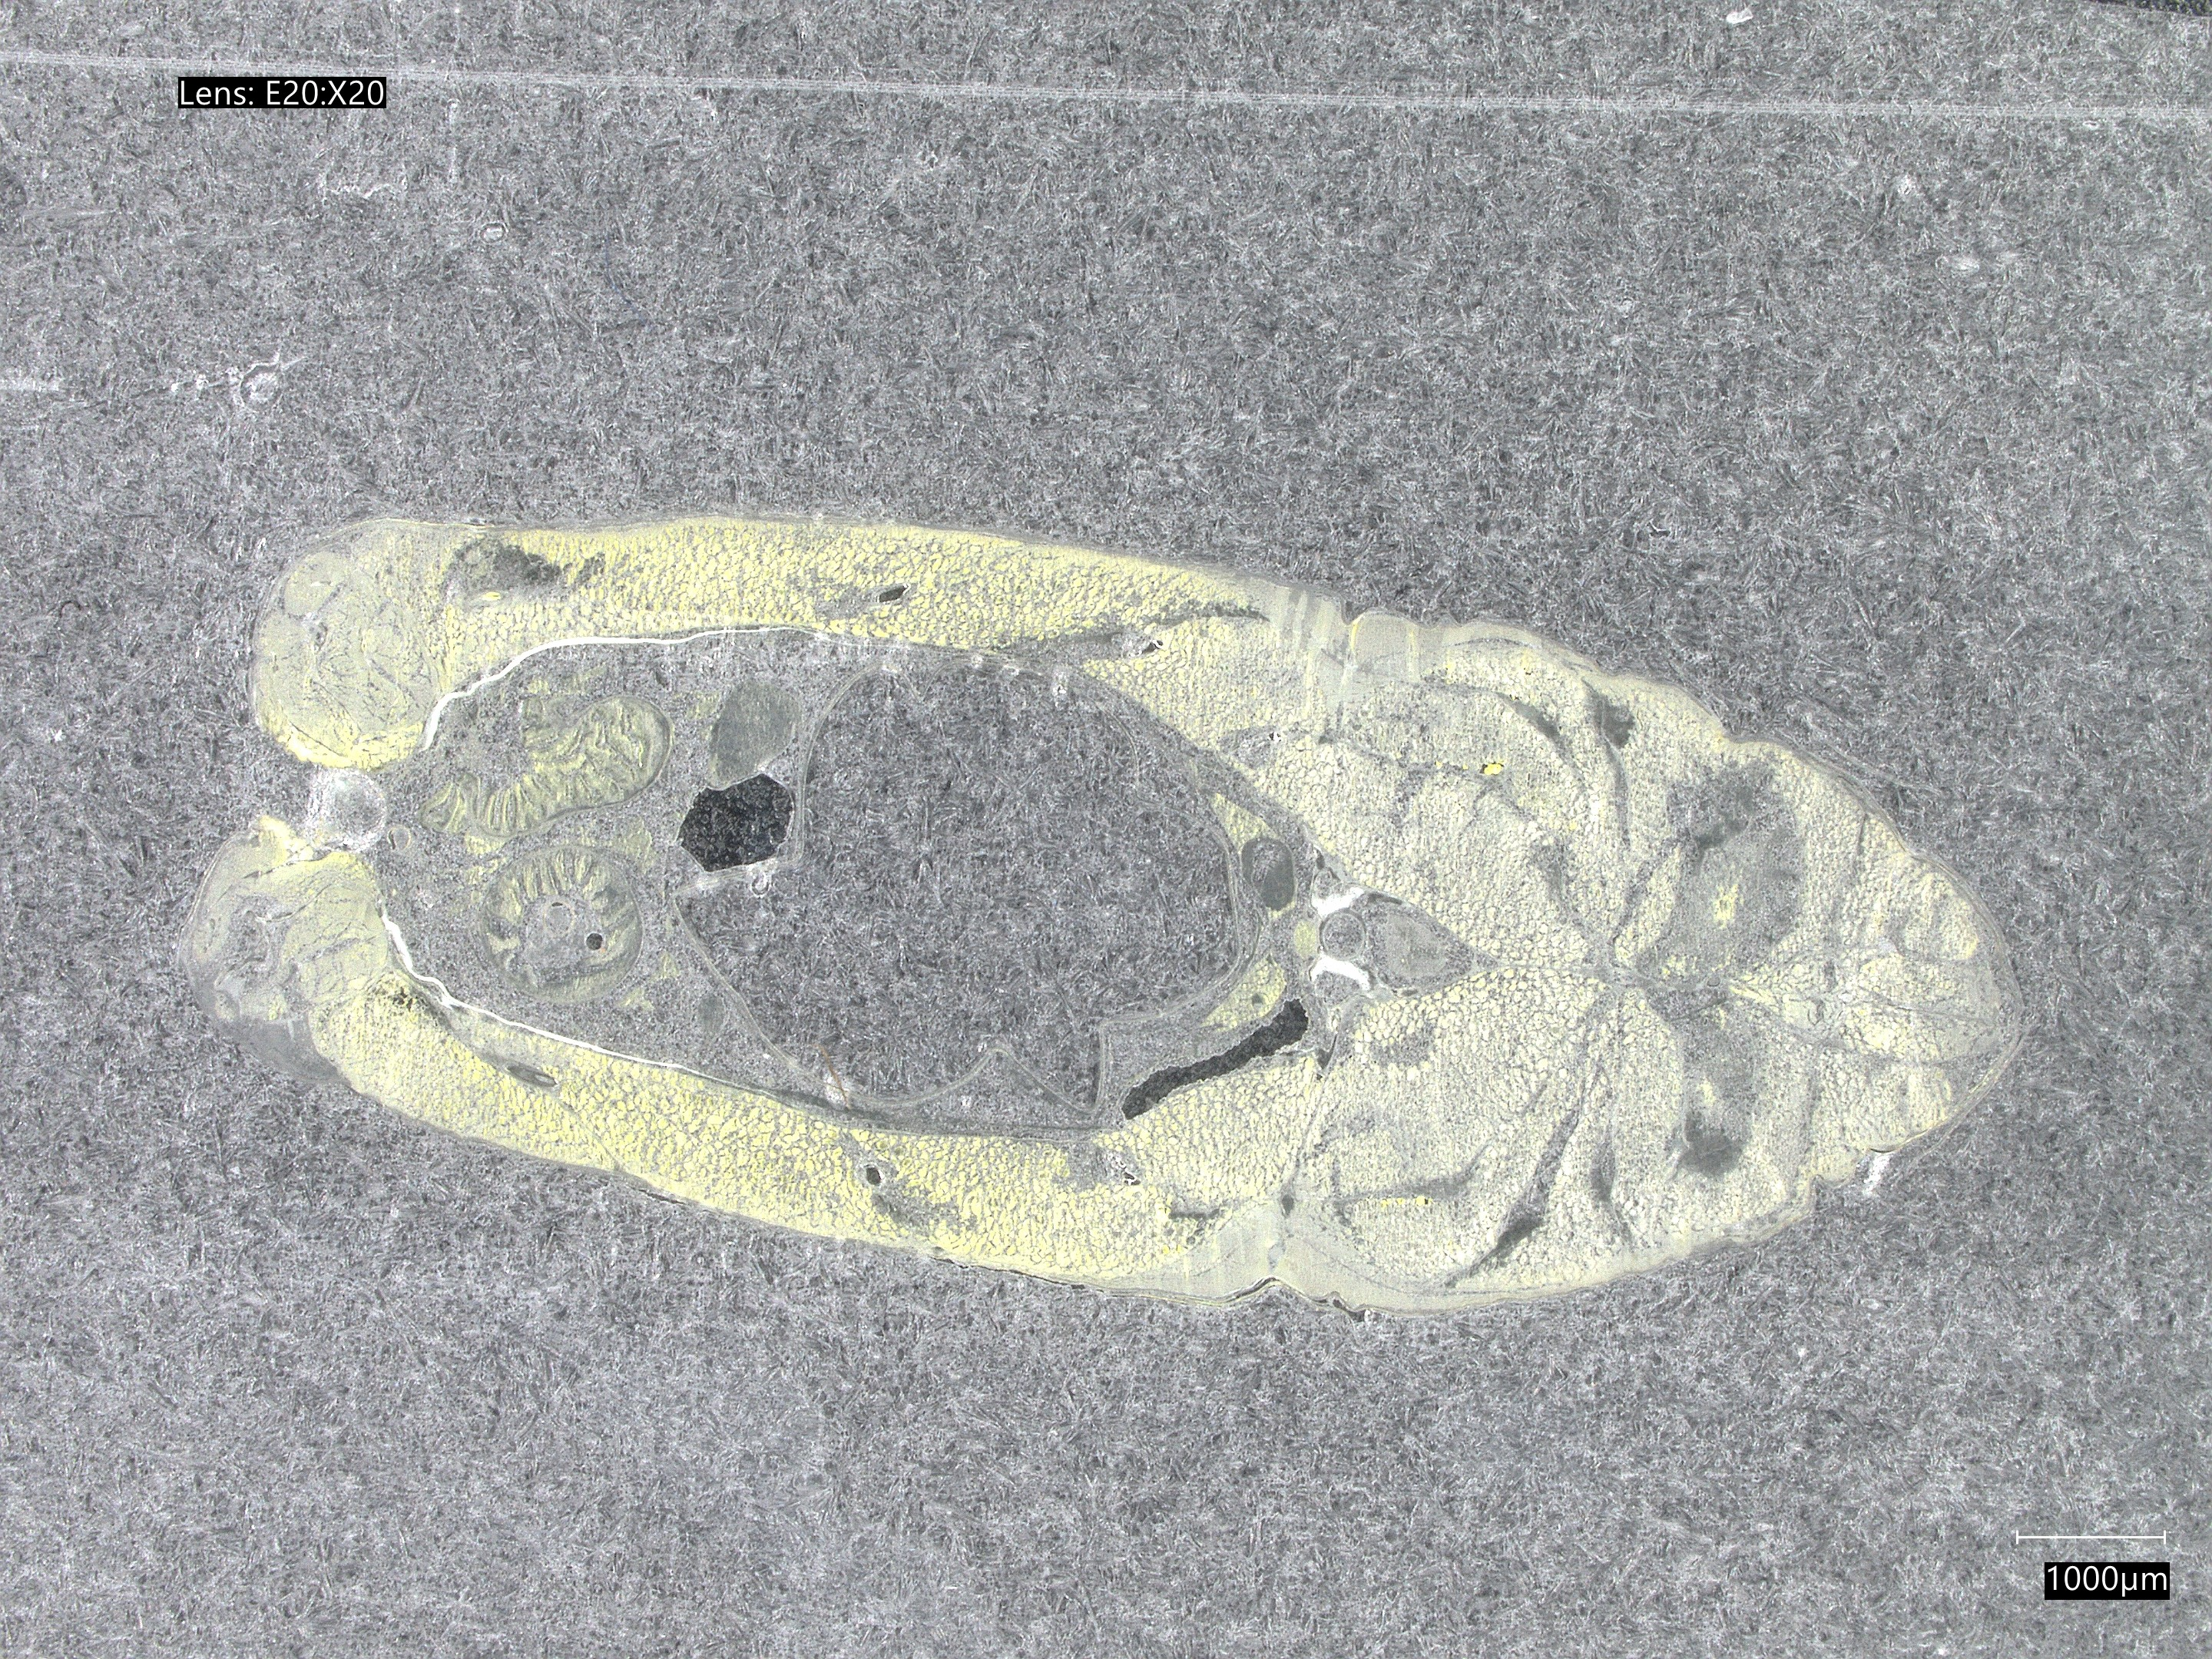
\includegraphics[width=0.8\textwidth]{./fig/sample9.5.jpg}
    \caption{切角9.5度的样本}
    \label{fig:sample9.5}
\end{figure}

对于这9组数据,需要找到的是在何种切角下,生物组织的完整度最高(质量最好)。因此现在需要将这9组数据根据生物组织的完整度进行重新标注。

根据刀片切割对生物组织的影响,我们将生物组织的完整度分为五个类别,分别为:horizental line, vertical line, slope, other, normal。其中horizental line代表显著的以水平白线为瑕疵的样本,vertical line代表显著的以竖直白线为瑕疵的样本,slope代表图像采集中存在明显的角度(不利于观察),other代表其他瑕疵(如采集中存在明暗显著差别的色块),normal代表正常的生物组织样本。这五类标签的示例图片如下所示。

\begin{figure}
    \centering
    \begin{minipage}{0.45\textwidth}
        \centering
        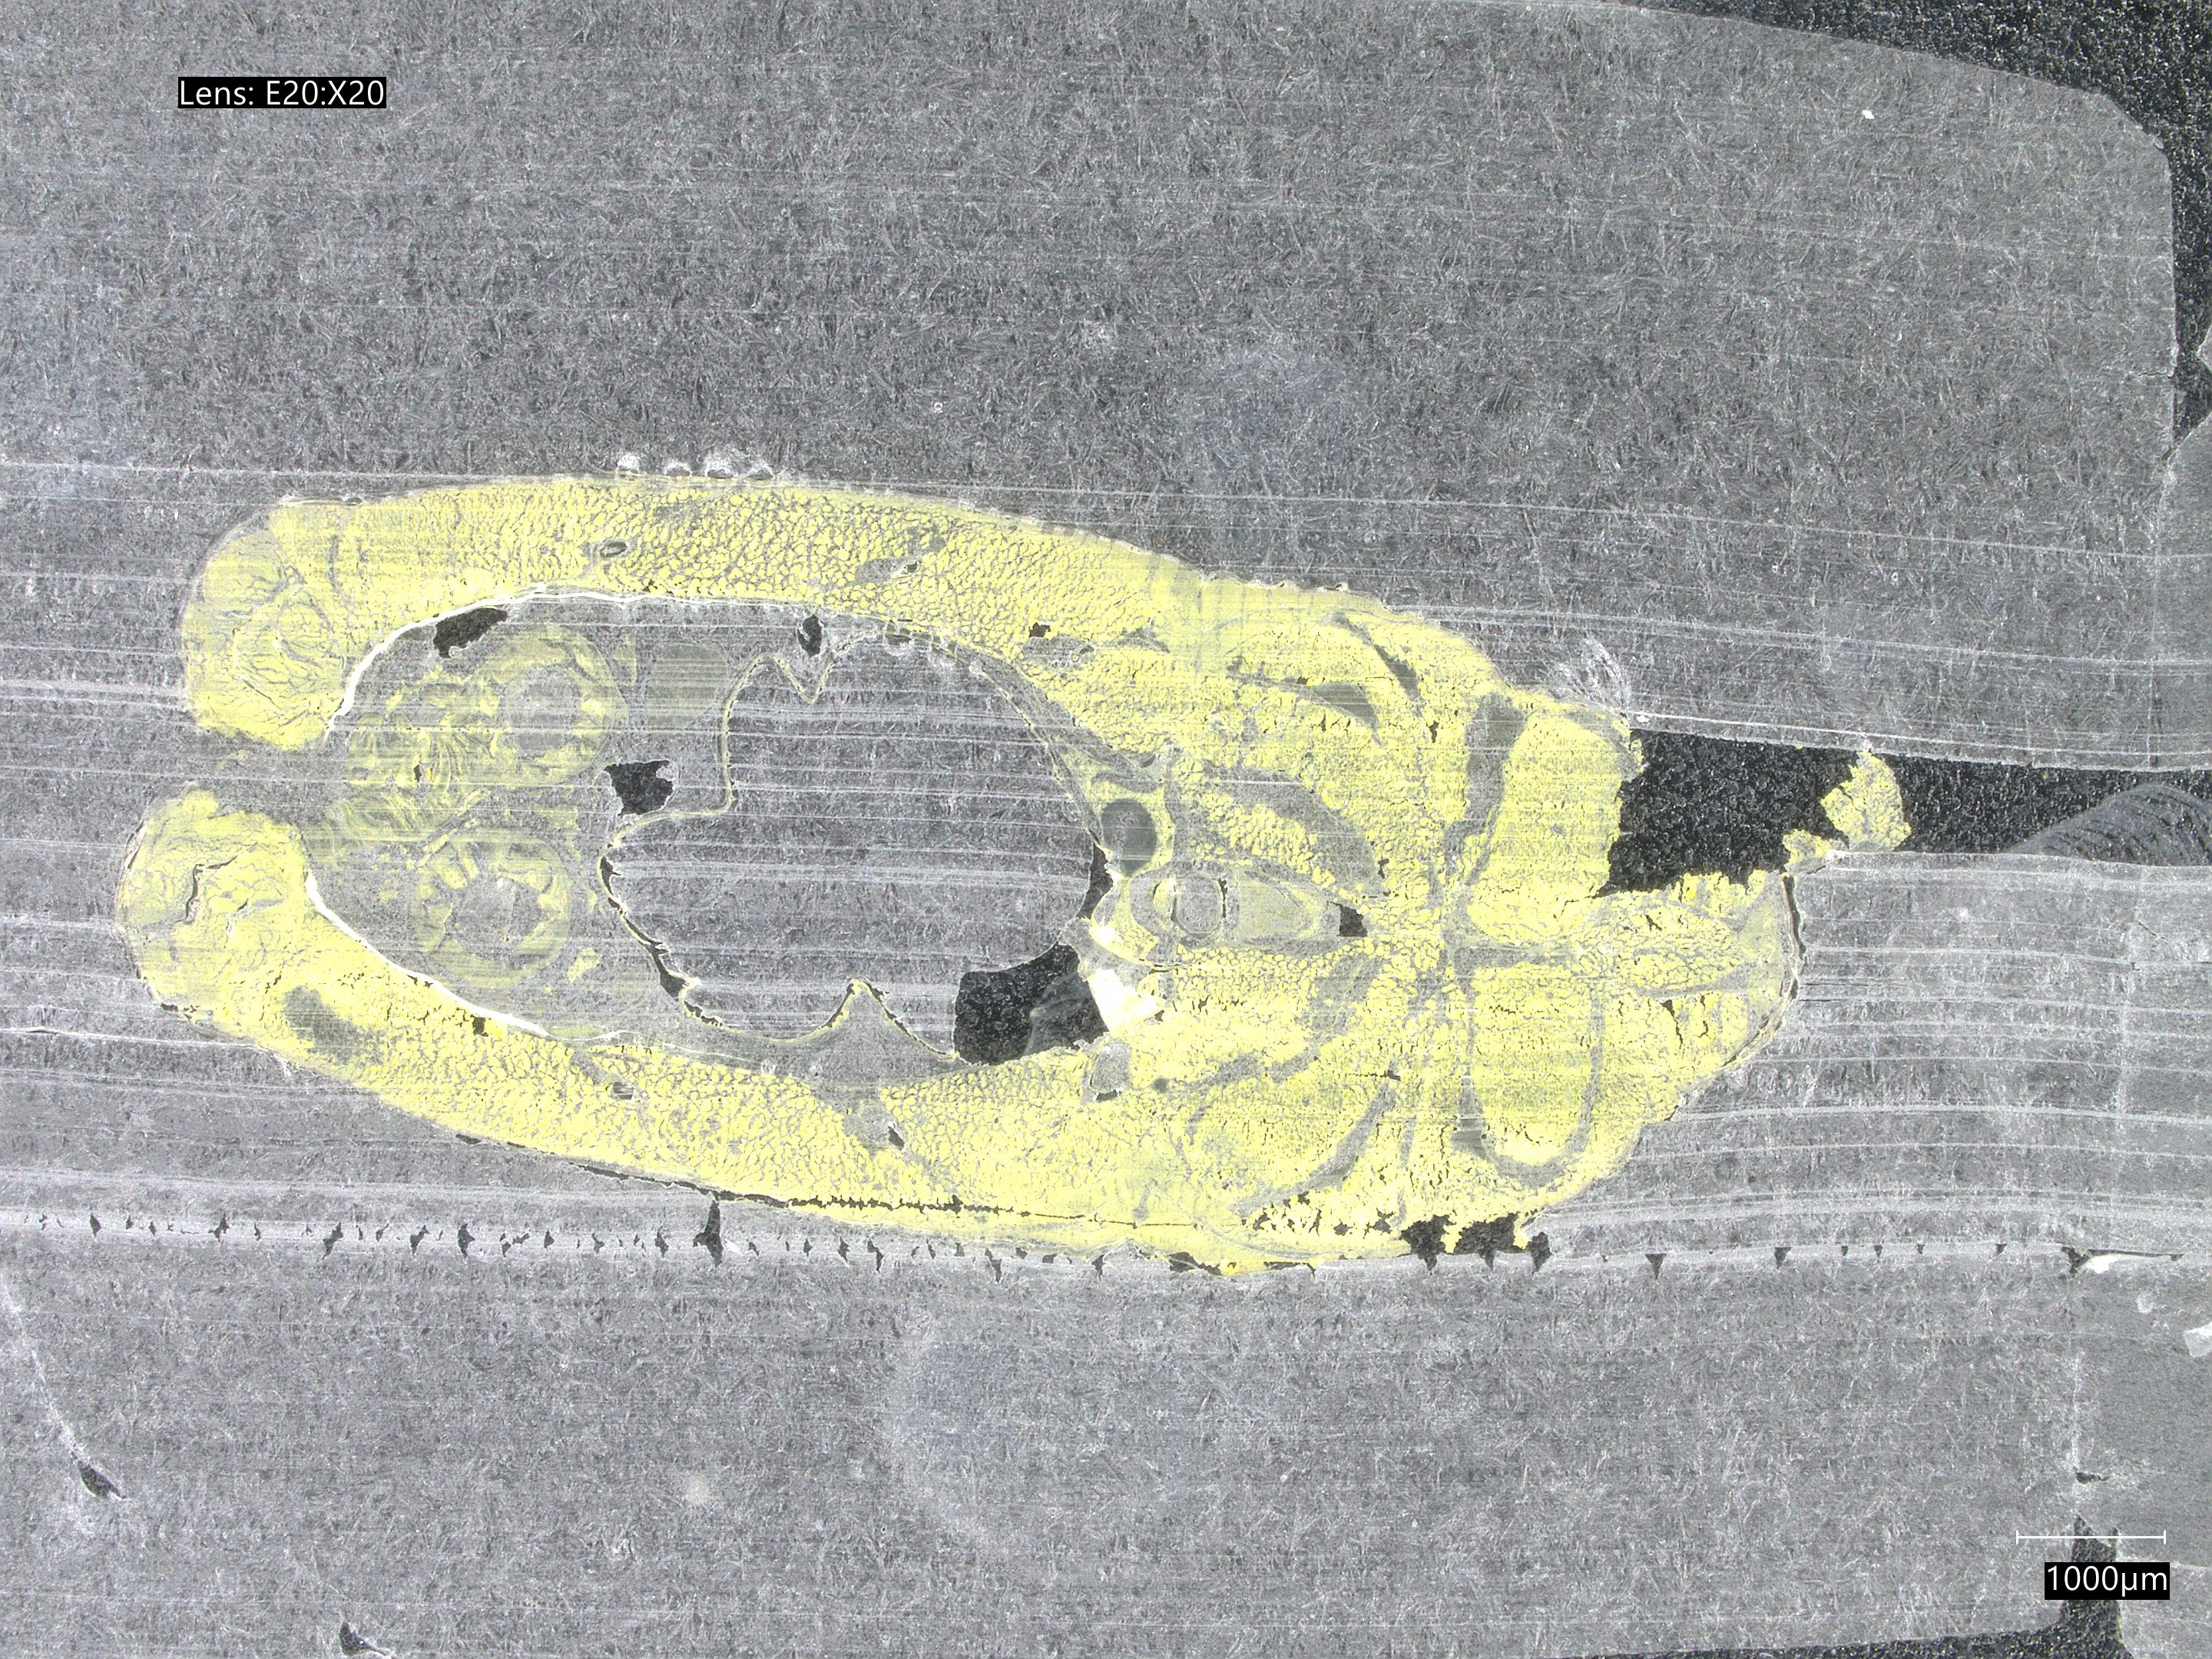
\includegraphics[width=\textwidth]{./fig/sample_1/horizental_line.jpg}
        \caption{horizental line}
        \label{fig:horizental_line}
    \end{minipage}
    \begin{minipage}{0.45\textwidth}
        \centering
        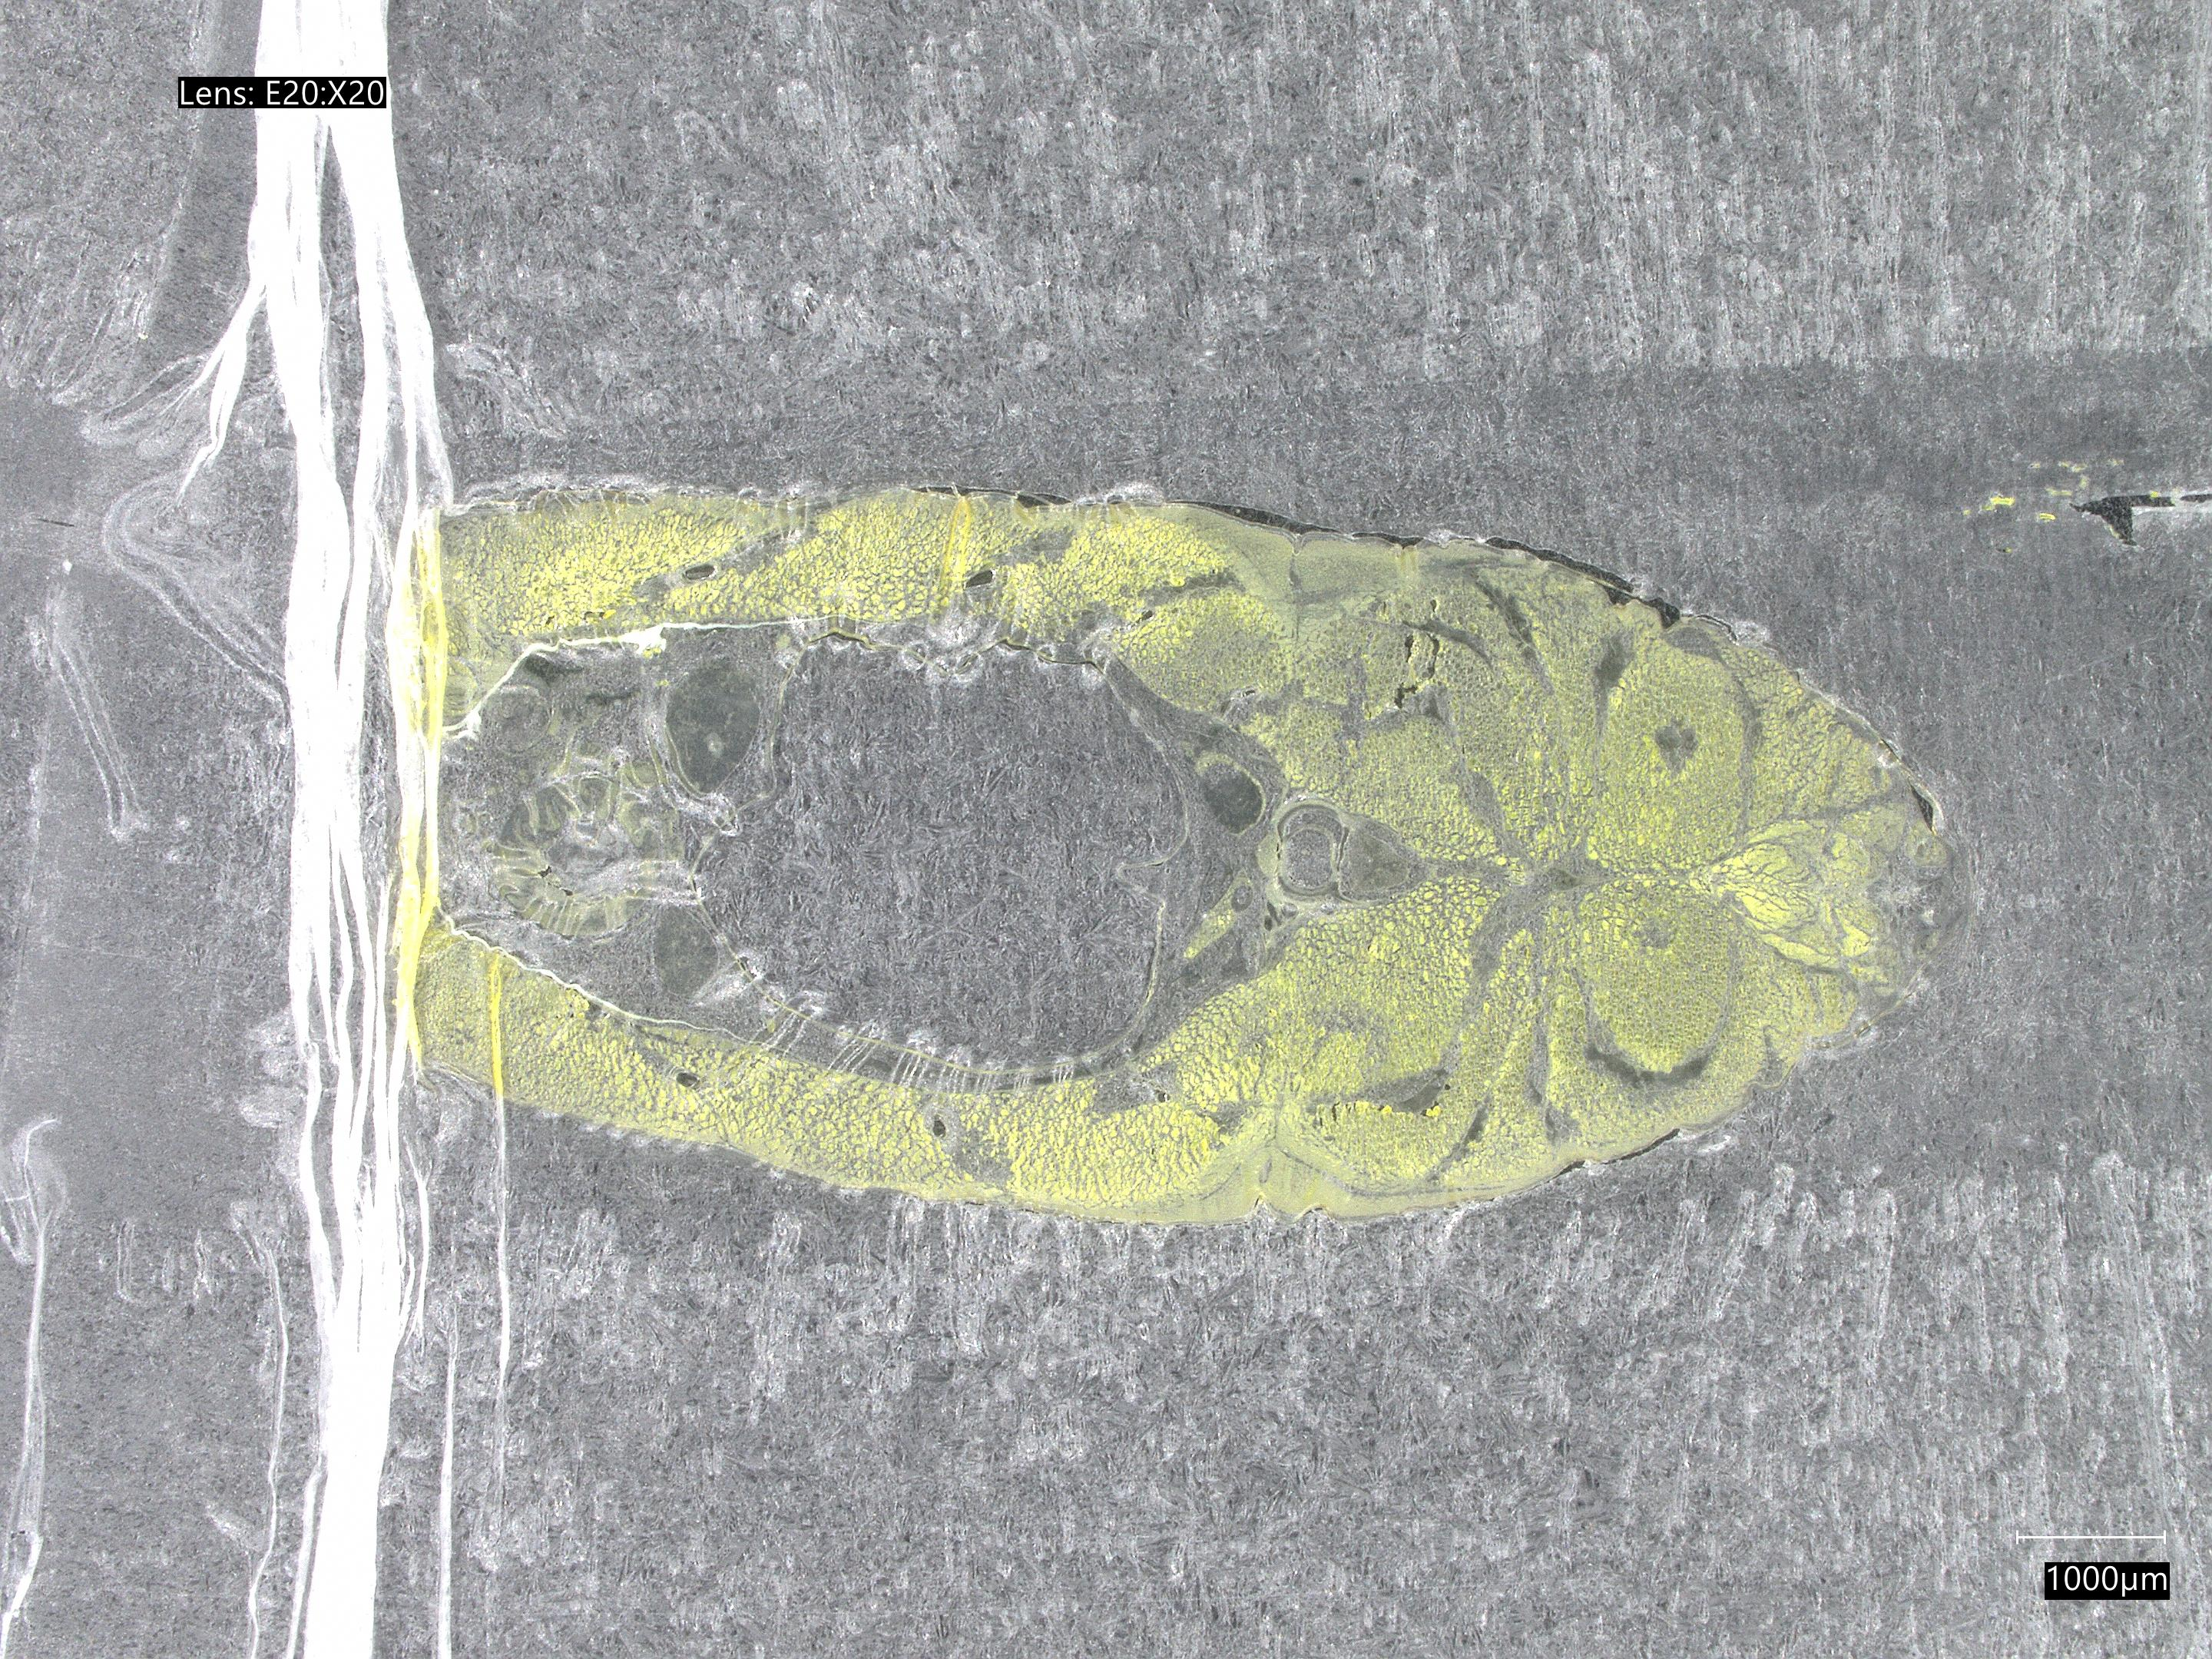
\includegraphics[width=\textwidth]{./fig/sample_1/vertical_line.jpg}
        \caption{vertical line}
        \label{fig:vertical_line}
    \end{minipage}
\end{figure}

\begin{figure}
    \centering
    \begin{minipage}{0.45\textwidth}
        \centering
        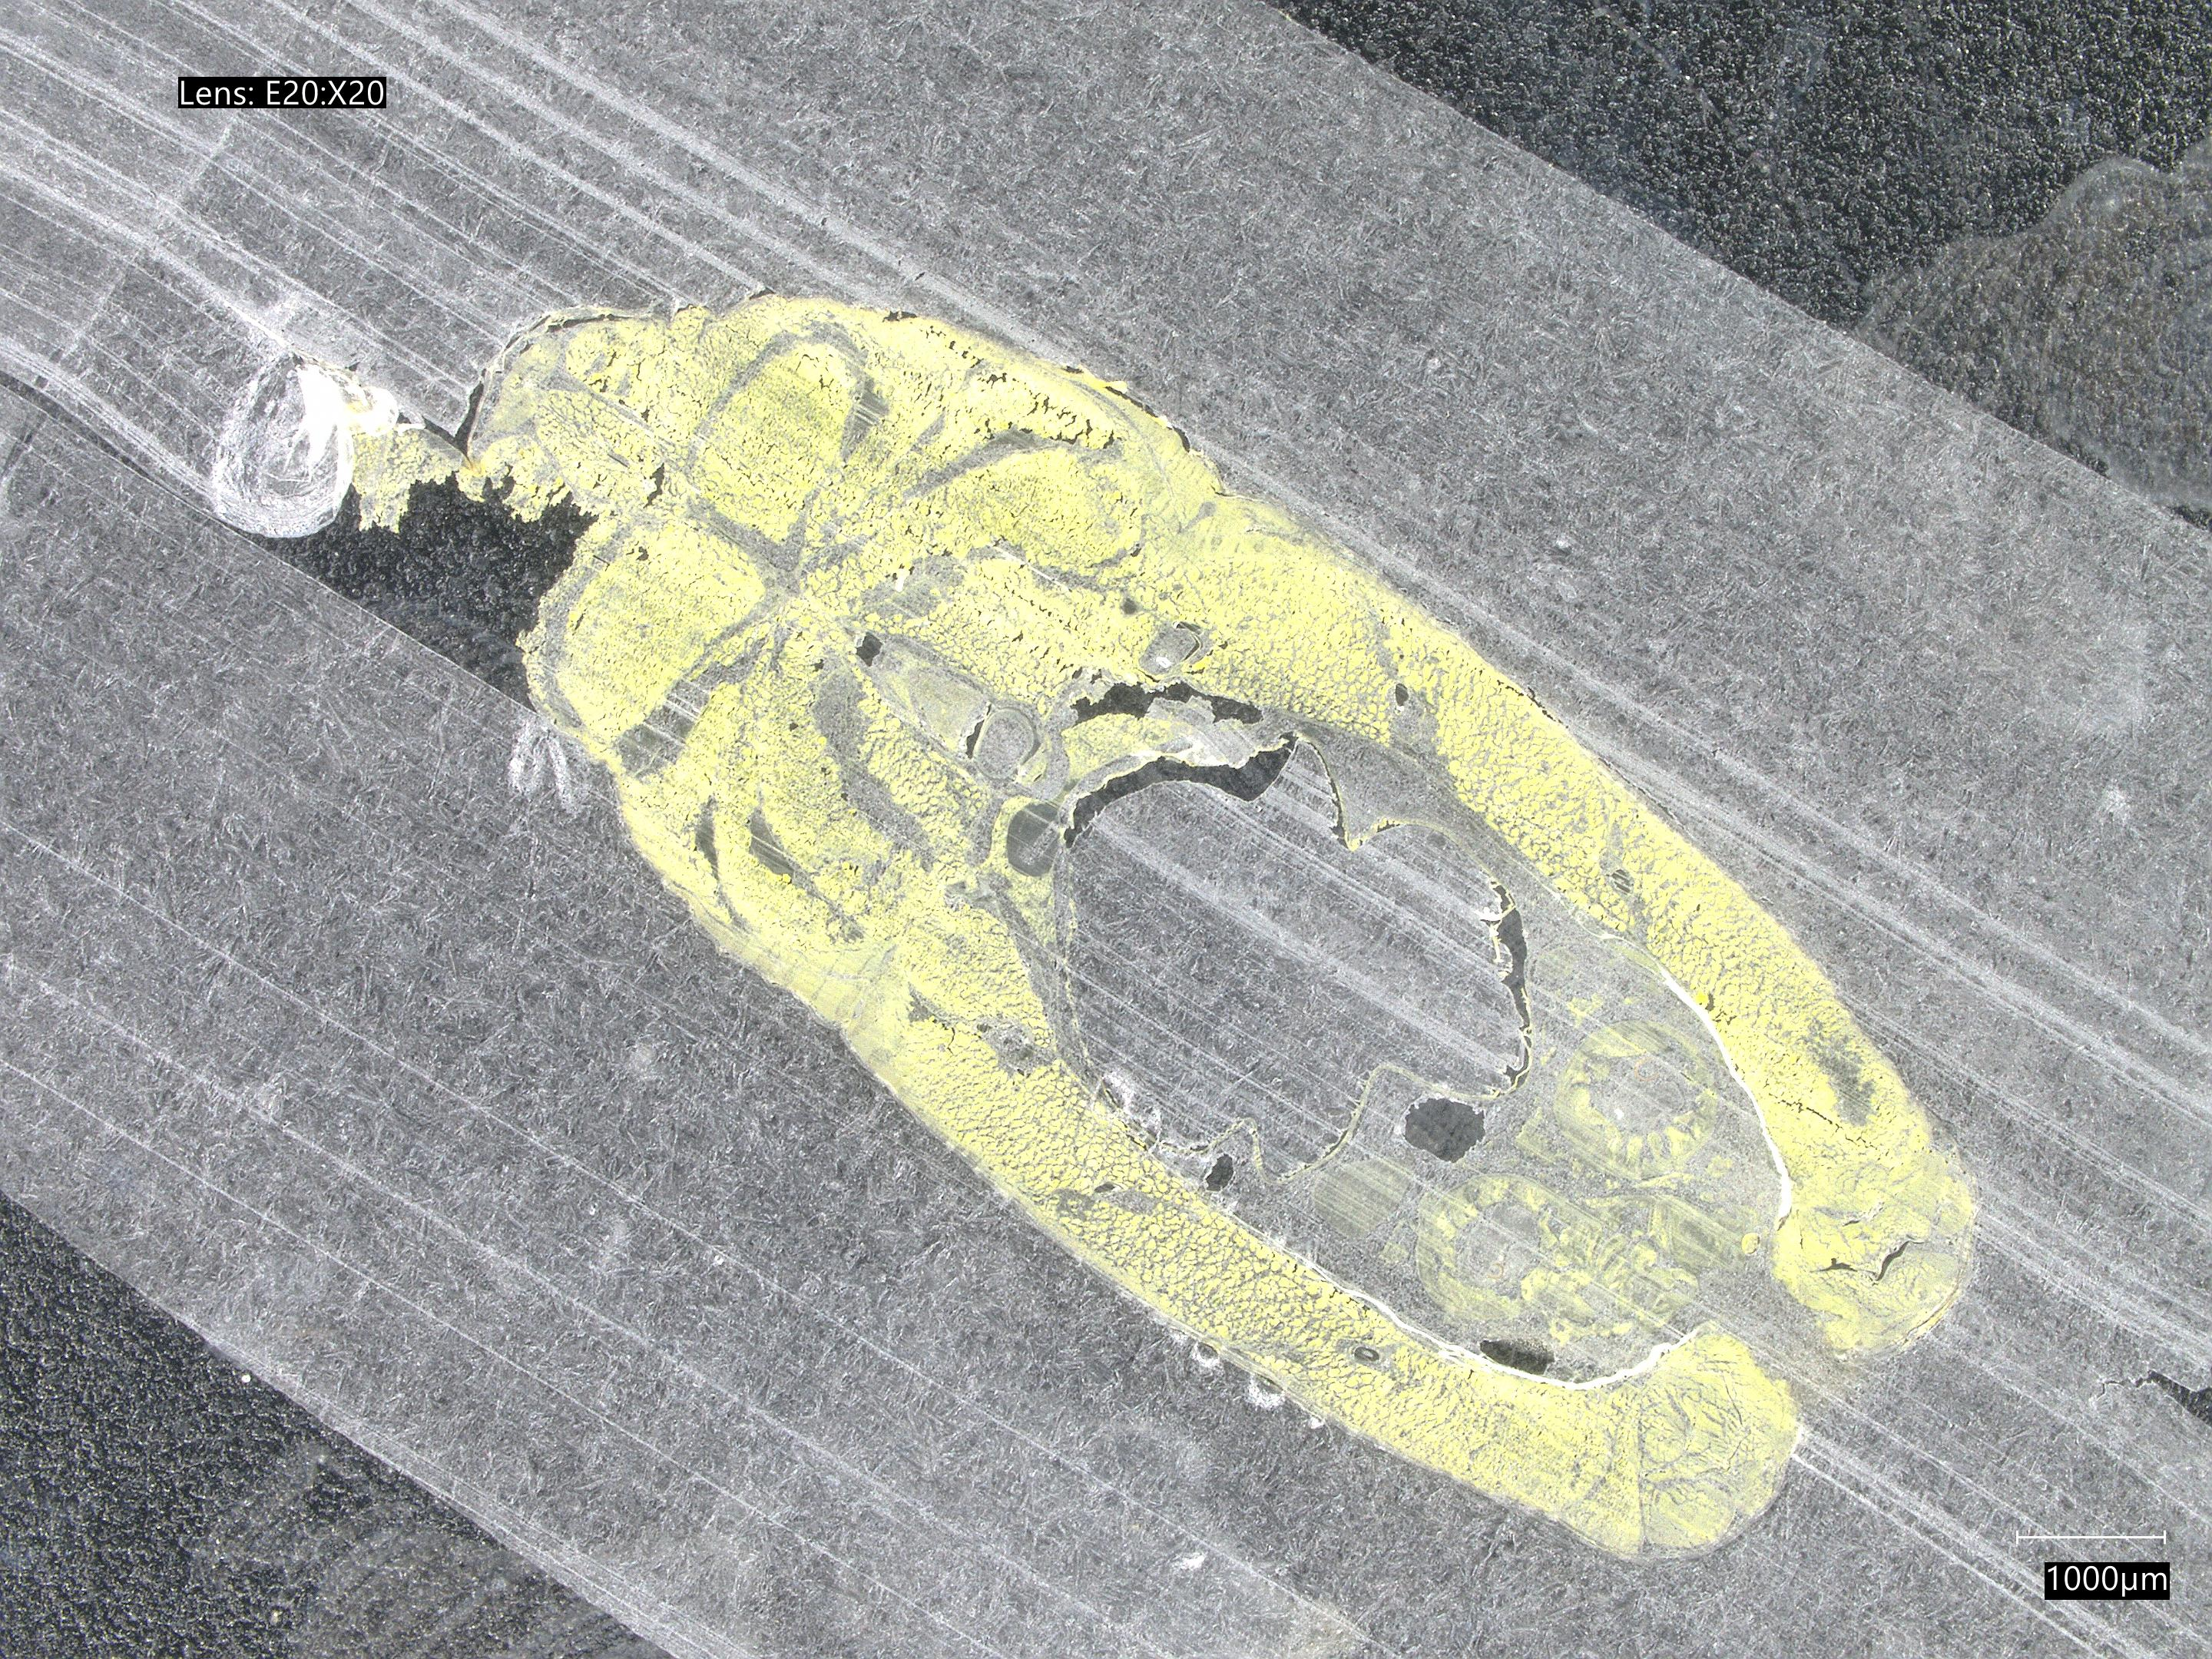
\includegraphics[width=\textwidth]{./fig/sample_1/slope.jpg}
        \caption{slope}
        \label{fig:slope}
    \end{minipage}
    \begin{minipage}{0.45\textwidth}
        \centering
        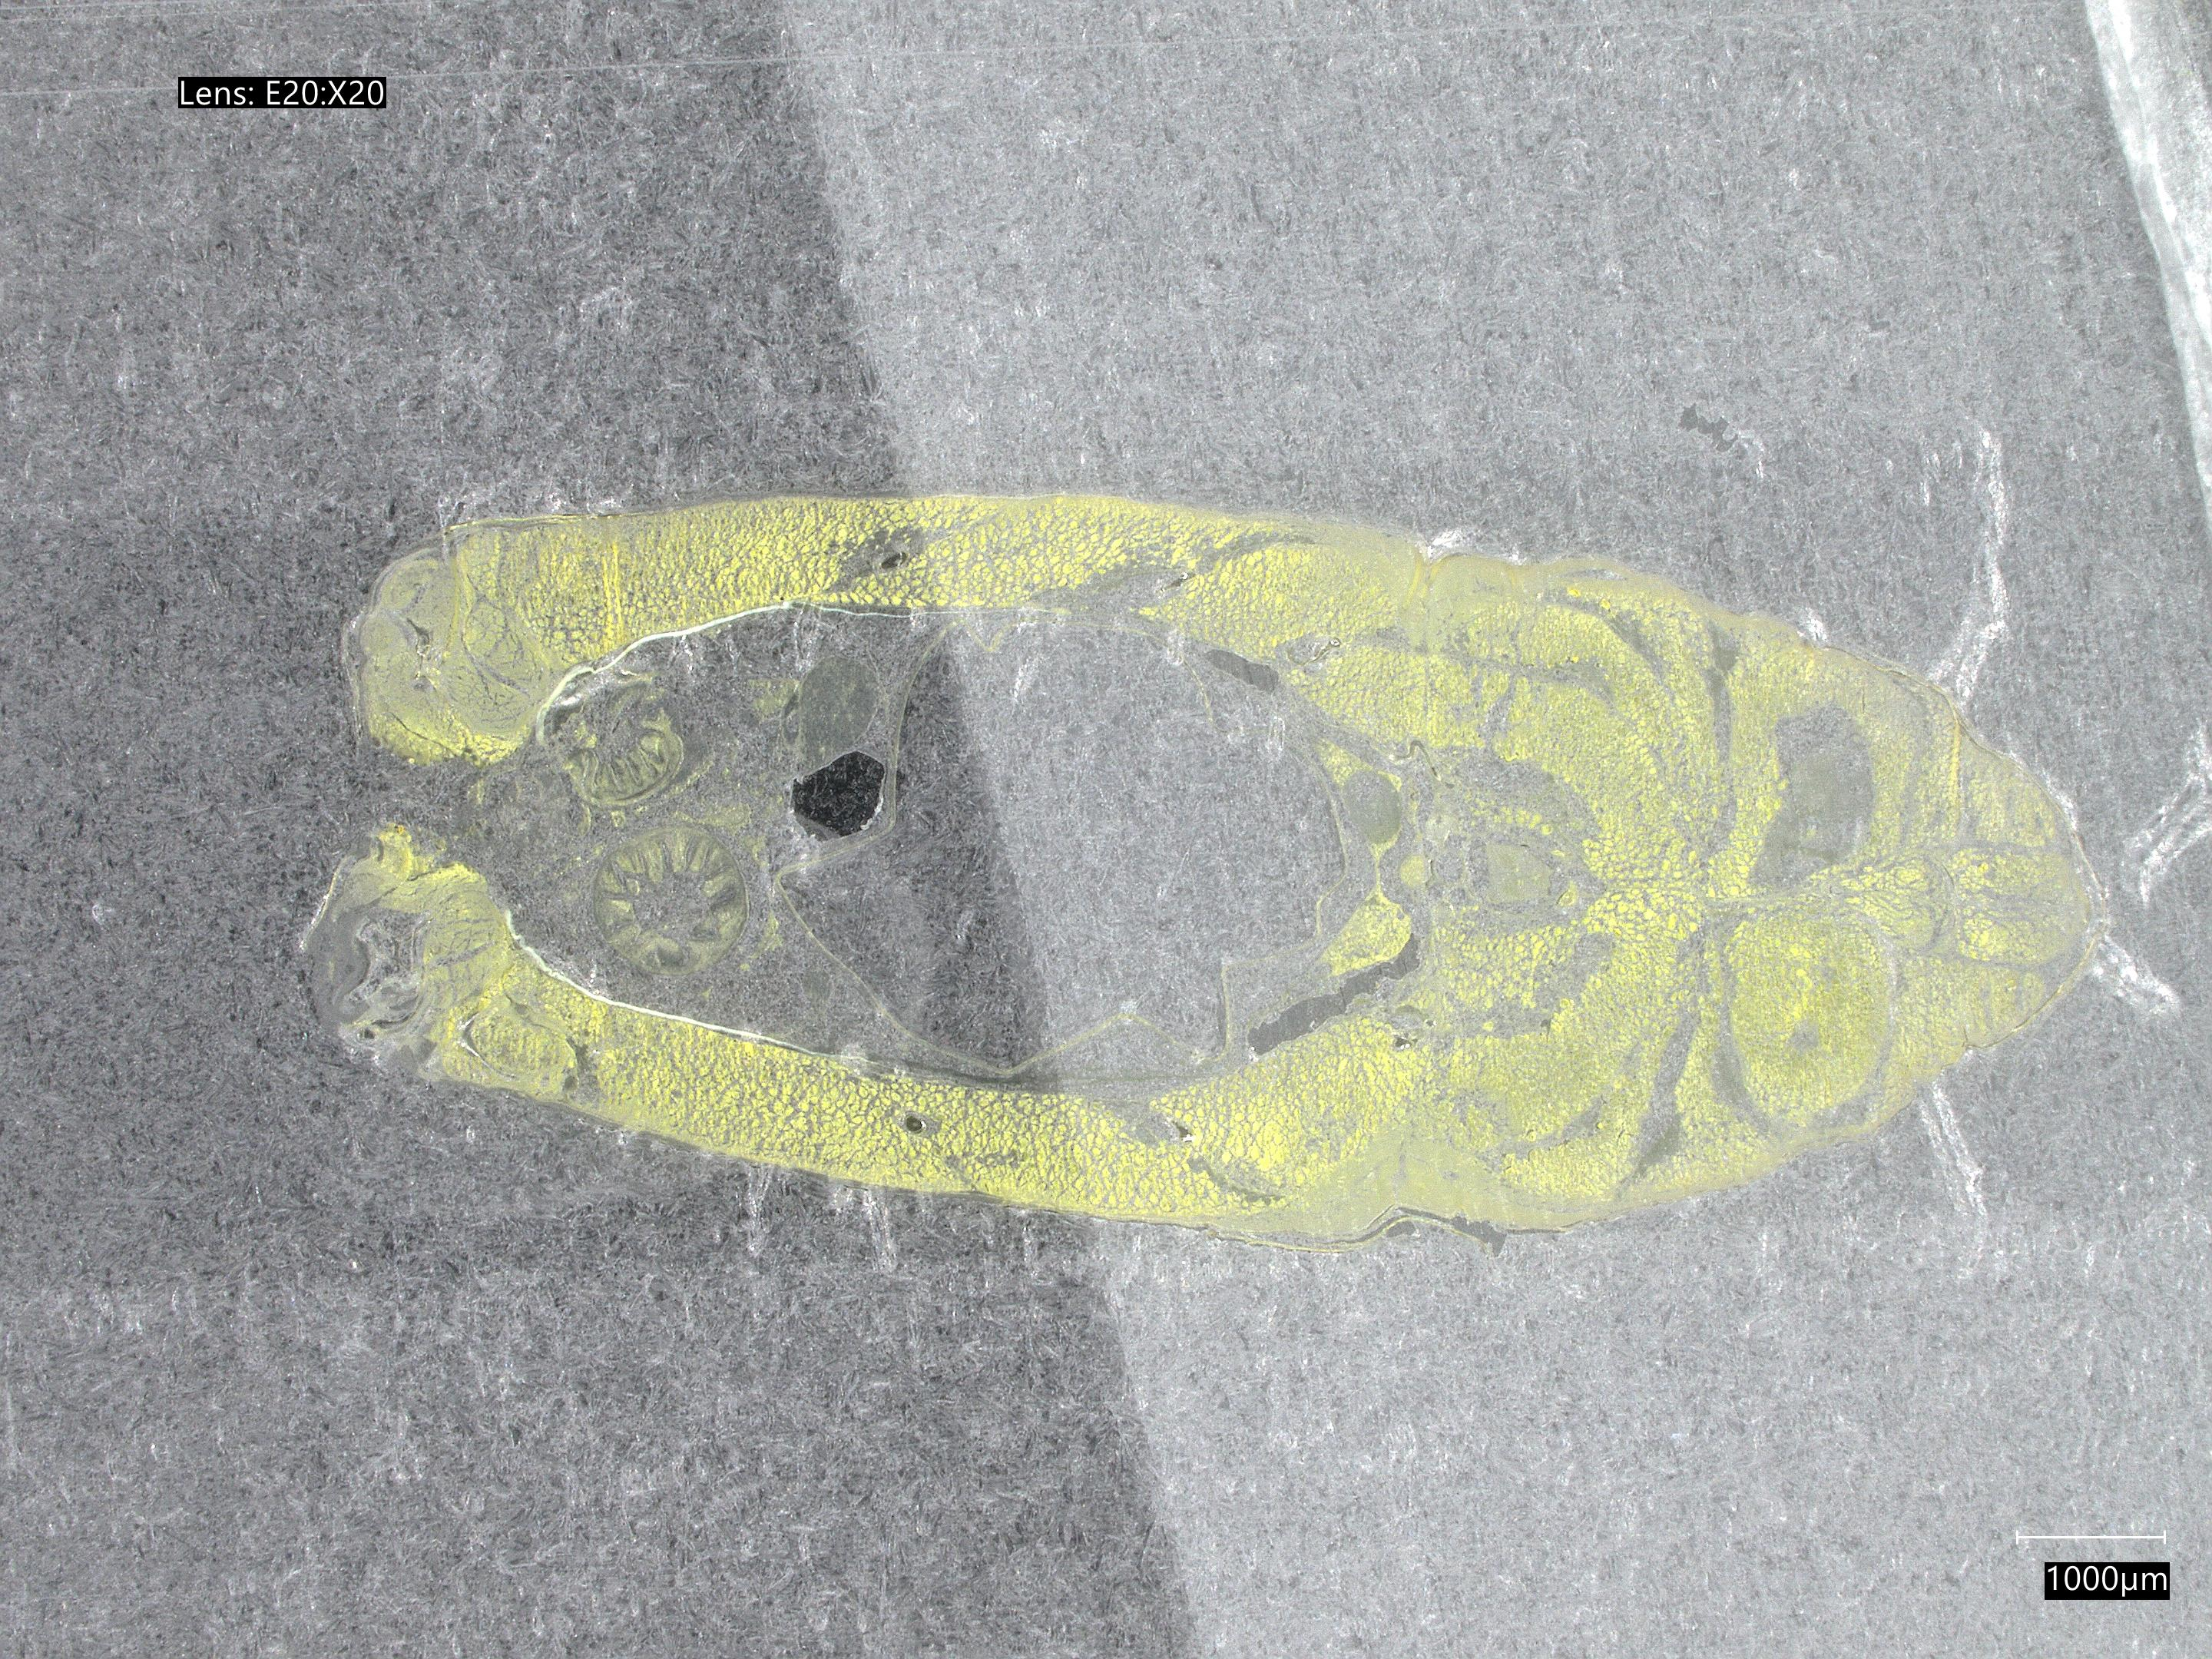
\includegraphics[width=\textwidth]{./fig/sample_1/other.jpg}
        \caption{other}
        \label{fig:other}
    \end{minipage}
\end{figure}

\begin{figure}
    \centering
    \begin{minipage}{0.45\textwidth}
        \centering
        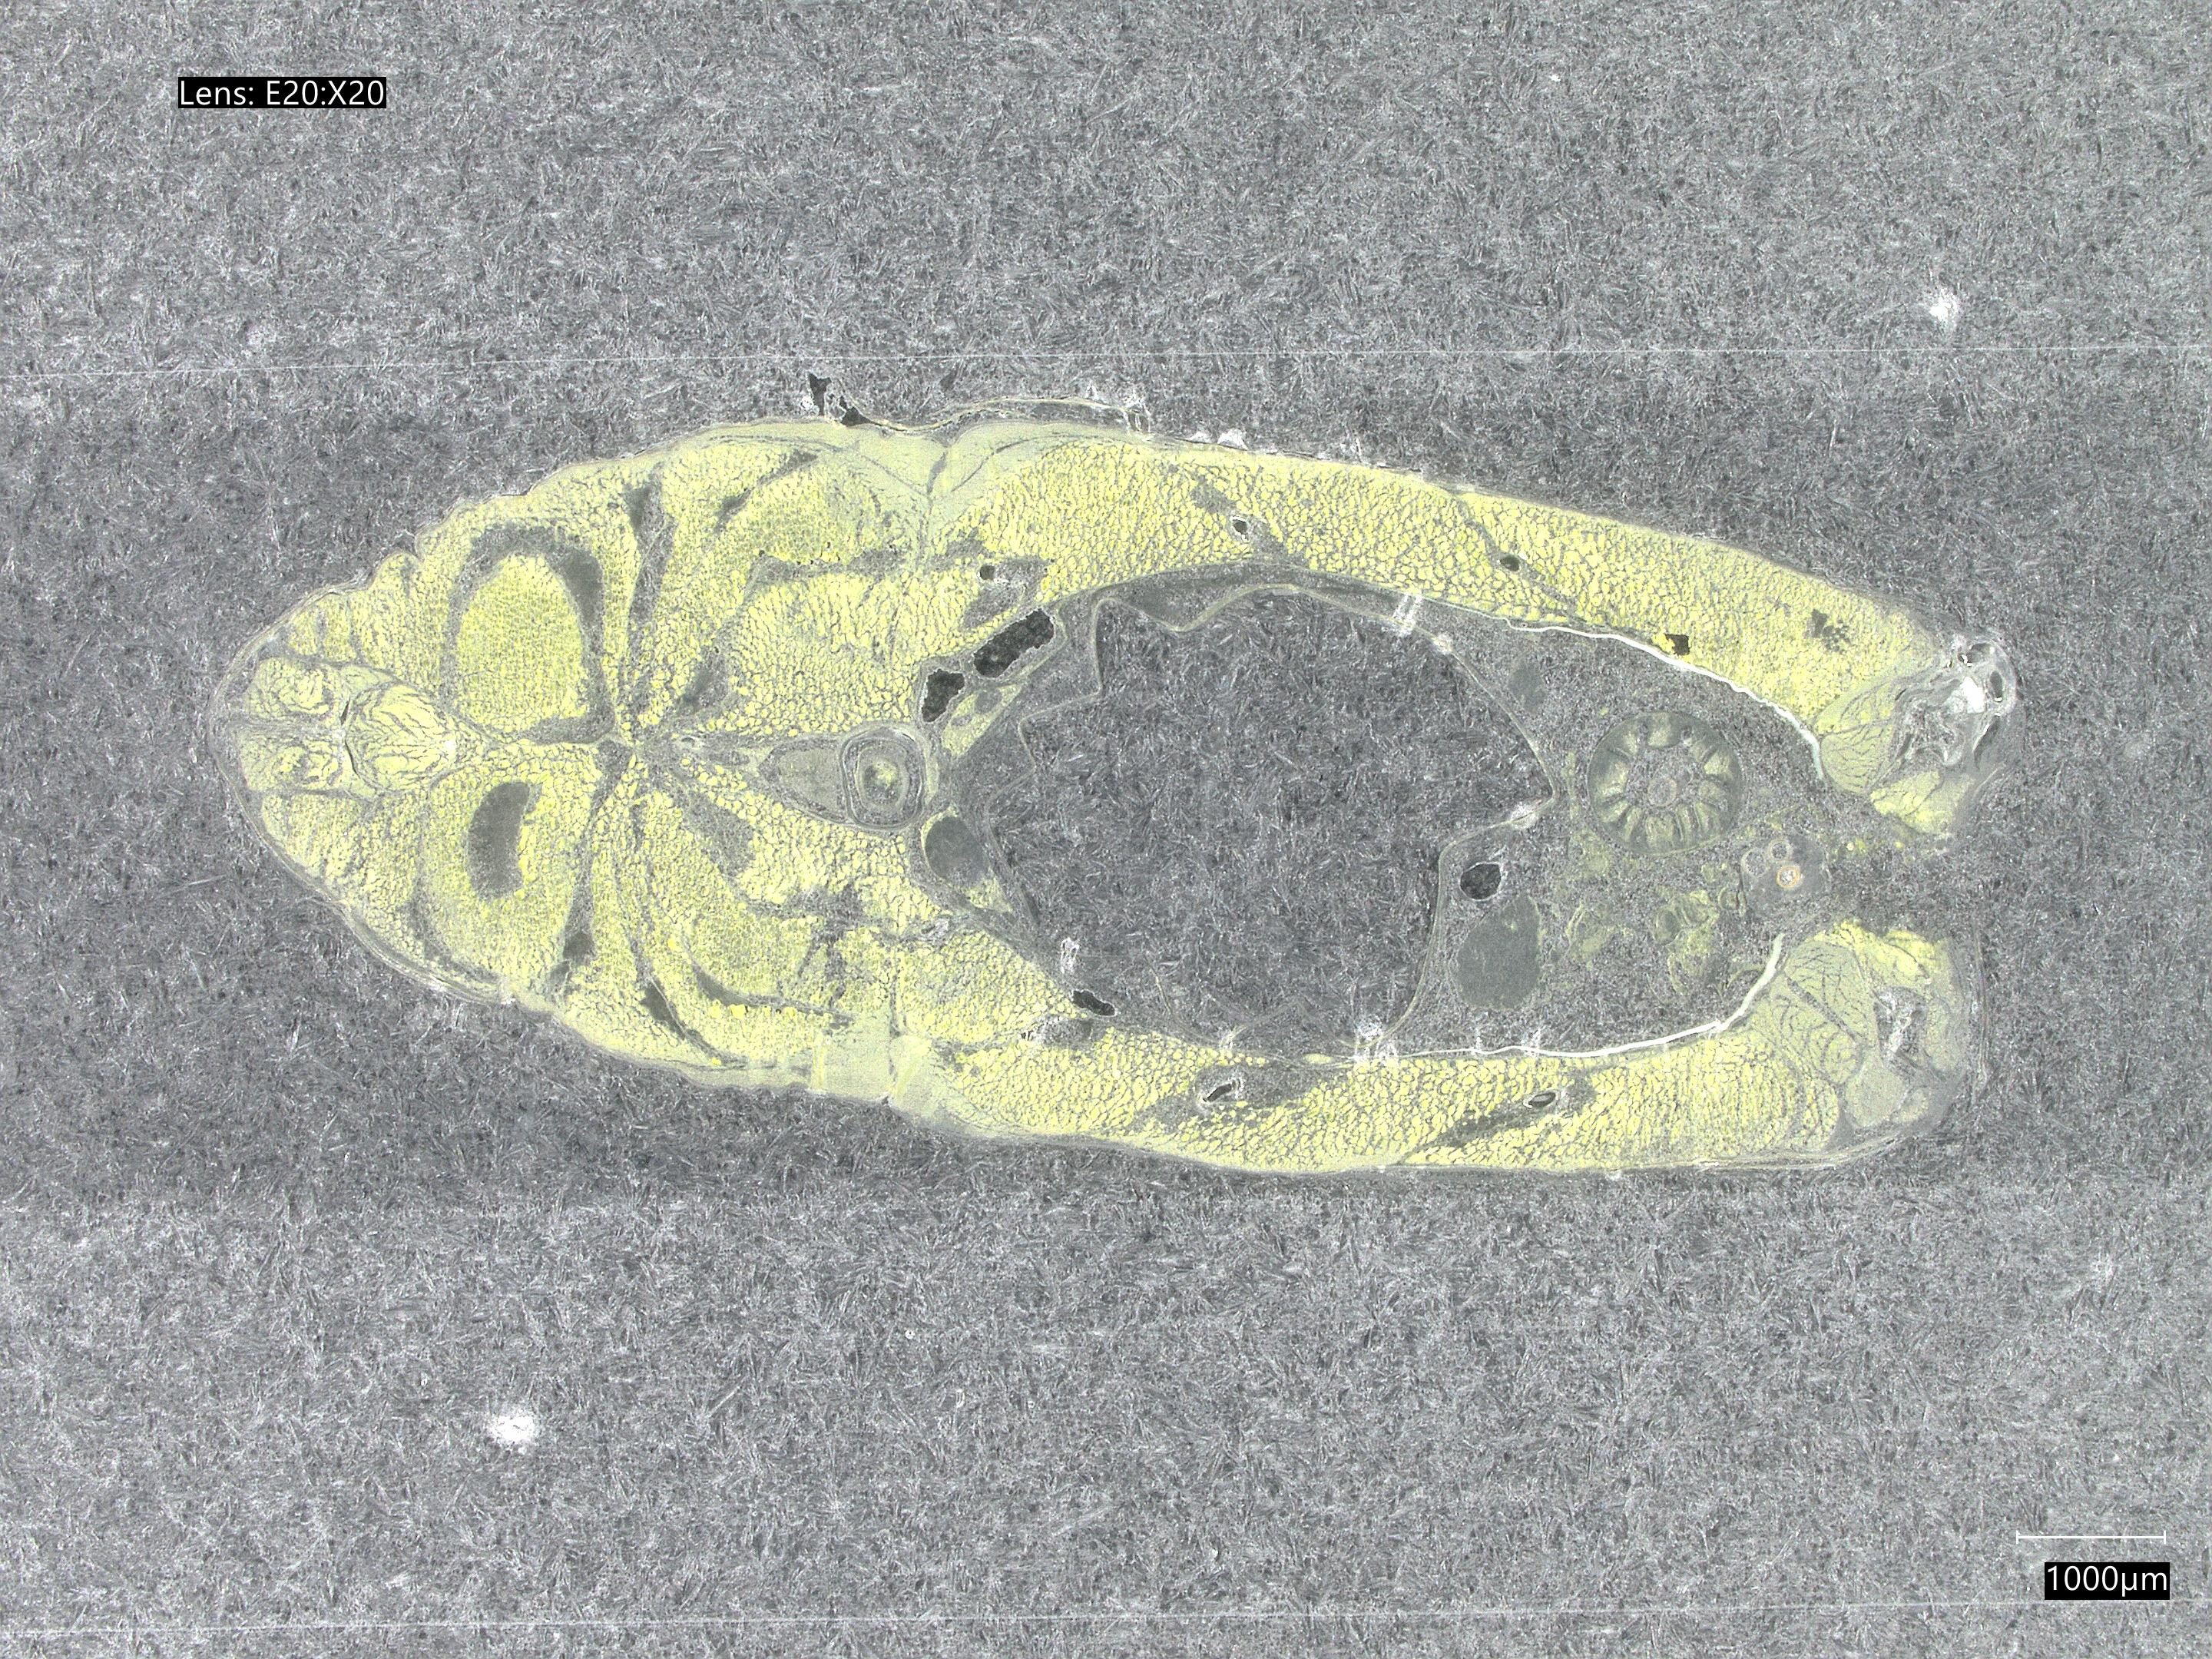
\includegraphics[width=\textwidth]{./fig/sample_1/normal.jpg}
        \caption{normal}
        \label{fig:normal}
    \end{minipage}
\end{figure}


对于每一张图片,我们需要将其标注为以上五个类别中的一个。这将作为我们的数据集,用于训练模型。


\FloatBarrier

\subsection{模型1:原始图像+简单的cnn网络}

对于一个全新的数据集,在不确定图像复杂度对应的何种模型之前,
首先尝试一个简单的cnn网络(架构如下),以了解数据集的特点和图像复杂度。

\begin{table}
\centering
\caption{Configuration of the simple CNN model}
\begin{tabular}{ccccc}
    \toprule
    \textbf{Layer Type} & \textbf{Configuration 1a} & \textbf{Configuration 1b} & \textbf{Configuration 1c} \\
    \midrule
    Input Layer & - & - & - \\
    Conv Layer 1 & Conv3-32 (relu) & Conv3-16 (relu) & Conv3-32 (relu) \\
    Pooling Layer 1 & MaxPooling & MaxPooling& MaxPooling \\
    Conv Layer 2 & Conv3-32 (relu) & Conv3-32 (relu) & Conv3-32 (relu) \\
    Pooling Layer 2 & MaxPooling & MaxPooling& MaxPooling \\
    Conv Layer 3 & Conv3-32 (relu) & Conv3-64 (relu) & Conv3-32 (relu) \\
    Pooling Layer 3 & MaxPooling & MaxPooling& MaxPooling \\
    Flattening Layer & Flatten() & Flatten() & Flatten() \\
    FC(Full connect) & Dense(128, relu) & Dense(128, relu) & Dense(256, relu) \\
    Output Layer & - & - & - \\
    \bottomrule
\end{tabular}
\label{tab:cnn_simple_configuration}
\end{table}

\autoref{tab:cnn_simple_configuration}显示的三个初始模型,分别为a,b,c。这三个模型的区别在于卷积层的数量和大小,全连接层的大小。a和b相比修改了卷积层的神经元数量,c相比a修改了全连接层的神经元数量。

数据的预处理部分,先将数据集分为训练集和测试集,其中训练集占80\%,测试集占20\%。之后将图像的长宽缩小一倍(即从2880*2160->1440*1080)并归一化数据。在训练过程中,我们使用了Adam优化器,交叉熵损失函数,使用早停。

下面图组展示了模型1a,1b,1c的准确度和损失随着训练次数的变化。

\begin{figure}
    \centering
    \begin{minipage}{0.45\textwidth}
        \centering
        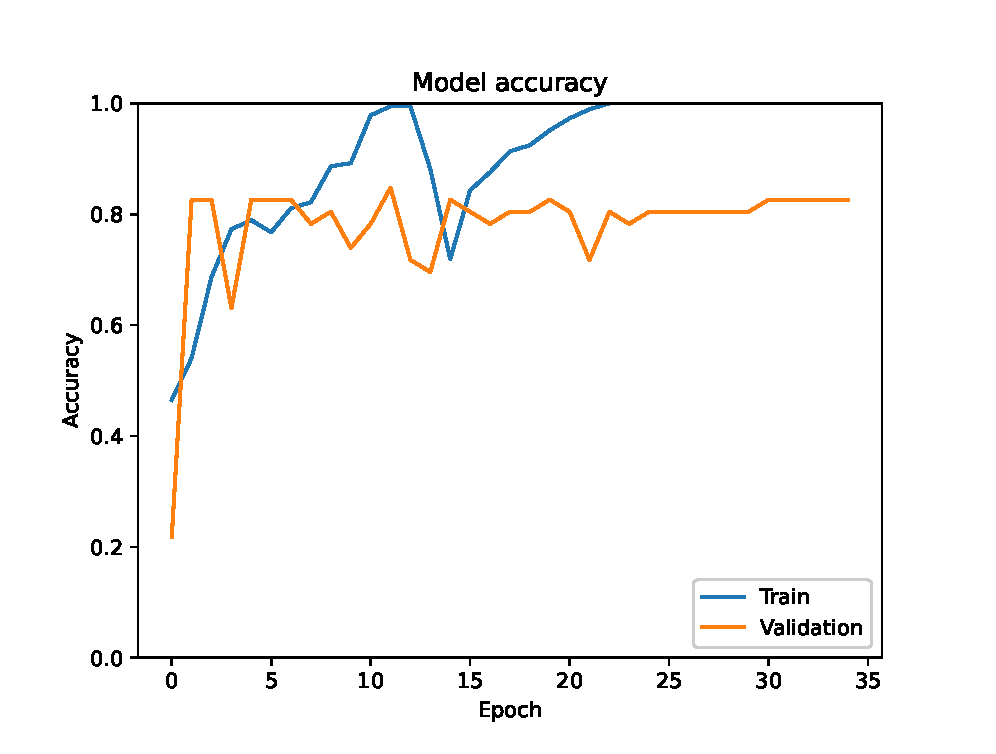
\includegraphics[width=\textwidth]{./fig/accuracy1a.eps}
        \caption{Model-1a accuracy}
        \label{fig:model1a_acc}
    \end{minipage}
    \begin{minipage}{0.45\textwidth}
        \centering
        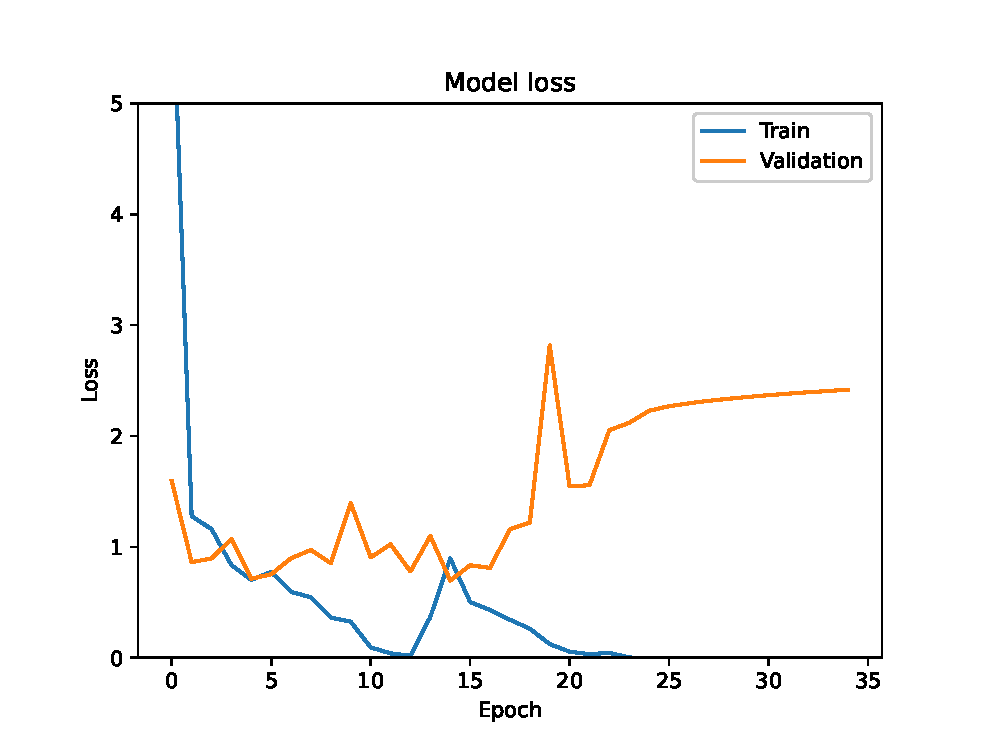
\includegraphics[width=\textwidth]{./fig/loss1a.eps}
        \caption{Model-1a loss}
        \label{fig:model1a_loss}
    \end{minipage}
\end{figure}

\begin{figure}
    \centering
    \begin{minipage}{0.45\textwidth}
        \centering
        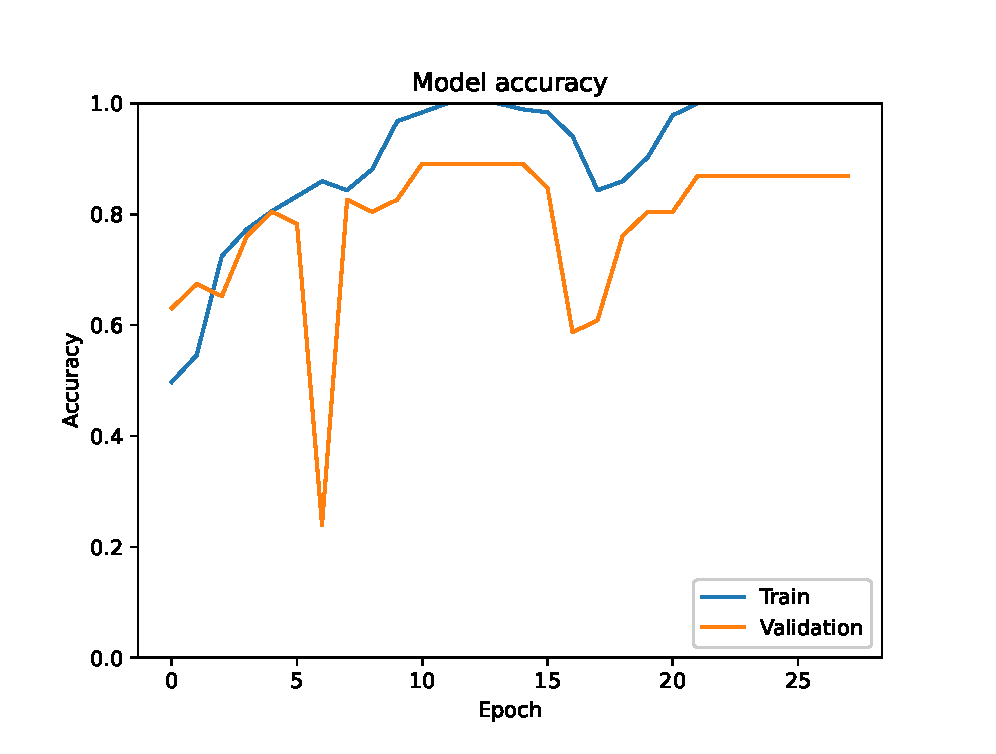
\includegraphics[width=\textwidth]{./fig/accuracy1b.eps}
        \caption{Model-1b accuracy}
        \label{fig:model1b_acc}
    \end{minipage}
    \begin{minipage}{0.45\textwidth}
        \centering
        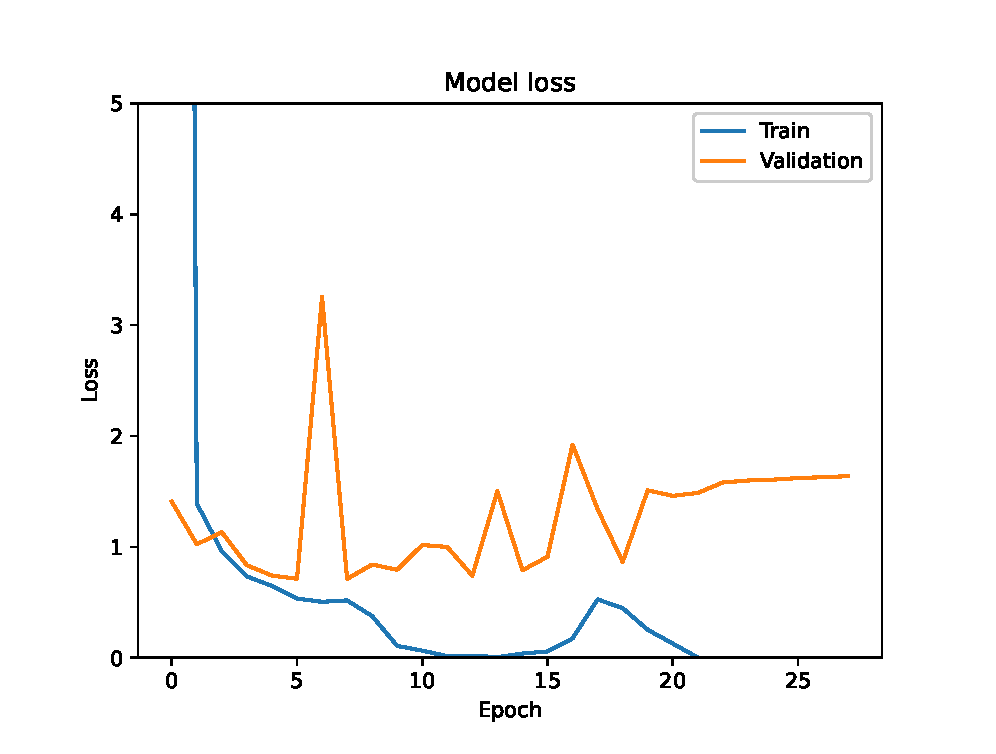
\includegraphics[width=\textwidth]{./fig/loss1b.eps}
        \caption{Model-1b loss}
        \label{fig:model1b_loss}
    \end{minipage}
\end{figure}

\begin{figure}
    \centering
    \begin{minipage}{0.45\textwidth}
        \centering
        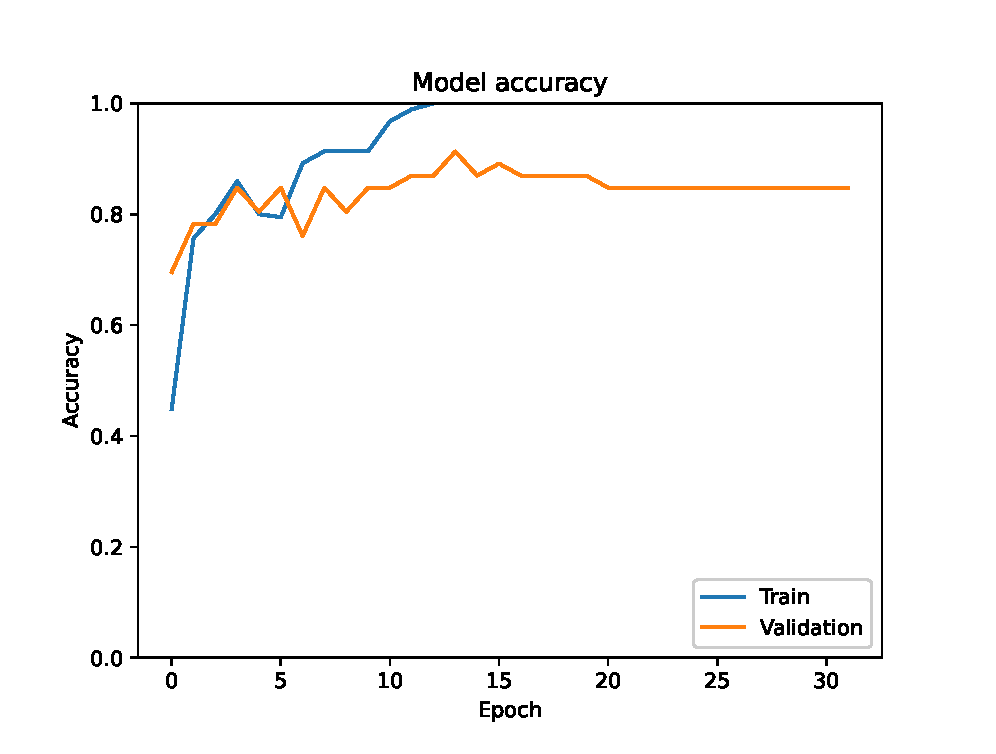
\includegraphics[width=\textwidth]{./fig/accuracy1c.eps}
        \caption{Model-1c accuracy}
        \label{fig:model1c_acc}
    \end{minipage}
    \begin{minipage}{0.45\textwidth}
        \centering
        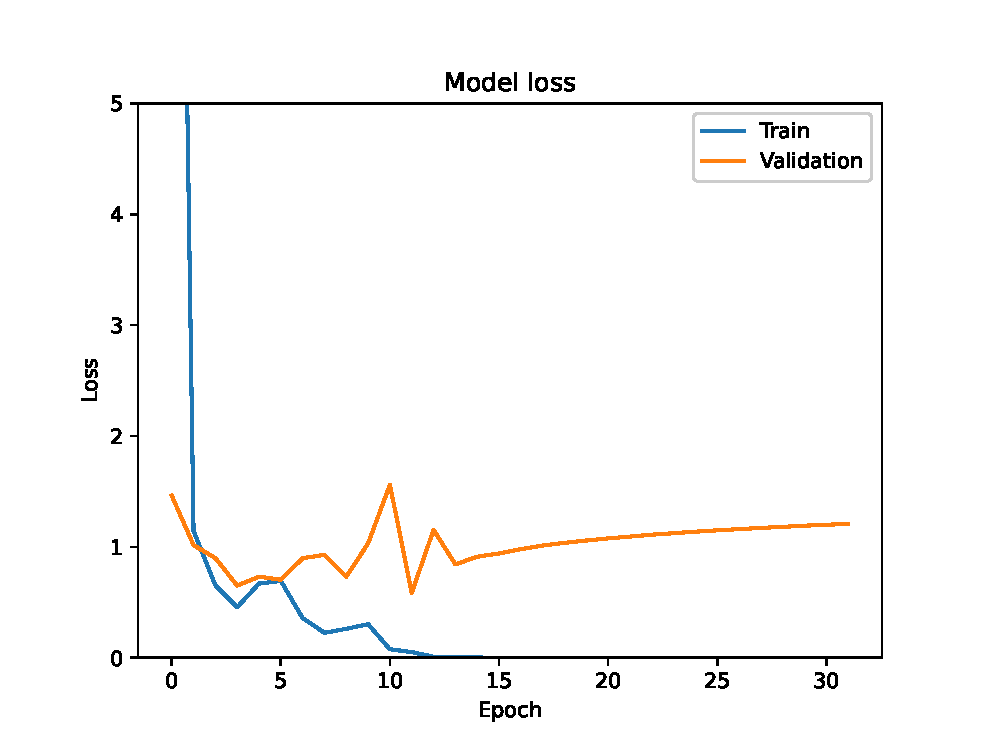
\includegraphics[width=\textwidth]{./fig/loss1c.eps}
        \caption{Model-1c loss}
        \label{fig:model1c_loss}
    \end{minipage}
\end{figure}

观察到模型1a,1b,1c的准确度和损失随着训练次数的变化,发现三个模型的训练准确度和损失都在不断趋于1和0,反应了模型的训练效果良好。但是在测试集上的准确度则是收敛于0.8-0.85左右,损失则收敛于大于1的值(模型1a甚至趋于2.5)。这说明模型在训练集上表现良好,但是在测试集上表现欠佳。其中模型1c是这三个模型里面验证损失最低的模型。这可能和数据量过小,模型过于简单(图像过于复杂)有关。可见模型不能很好的泛化到验证集上。


%具体的测试集测试在第五章

\FloatBarrier


\subsection{改进:图片预处理}

在模型表现能力欠佳的情况下,我们考虑是否是图像过于复杂导致模型难以提取出显著特征。因此我们考虑对图像进行预处理,以突出图像中我们希望让计算机识别的特征,并且在一定程度上去除图像的无关特征和噪声,以提高后续的深度学习模型的准确性。


在这里采用边缘检测,阈值分割两种方法对图像进行预处理。


\subsubsection{边缘检测}

正如在3.1.1中所提到的,边缘检测的原理是通过检测像素点的灰度值的变化(梯度)来确定图像中的边缘。假定原始图像是\autoref{fig:sample9.5}.

在进行边缘检测之前,还需要进行一步前处理-高斯模糊。这么做的原因是,高斯模糊可以减少图像中的噪声,平滑图像的梯度,减小识别假边缘的几率,使得边缘检测更加准确。(https://ieeexplore.ieee.org/abstract/document/6044249)在高斯模糊核的选择上,选择高斯核分别为21,41,61,81(图像宽度的1\%,2\%,3\%,4\%)。
高斯模糊后的图像如下所示。为了方便更直观的展示高斯模糊核对边缘检测的影响,这里采用sobel算子计算经过高斯模糊后的边缘并手动提亮50。

\begin{figure}
    \centering
    \begin{minipage}{0.45\textwidth}
        \centering
        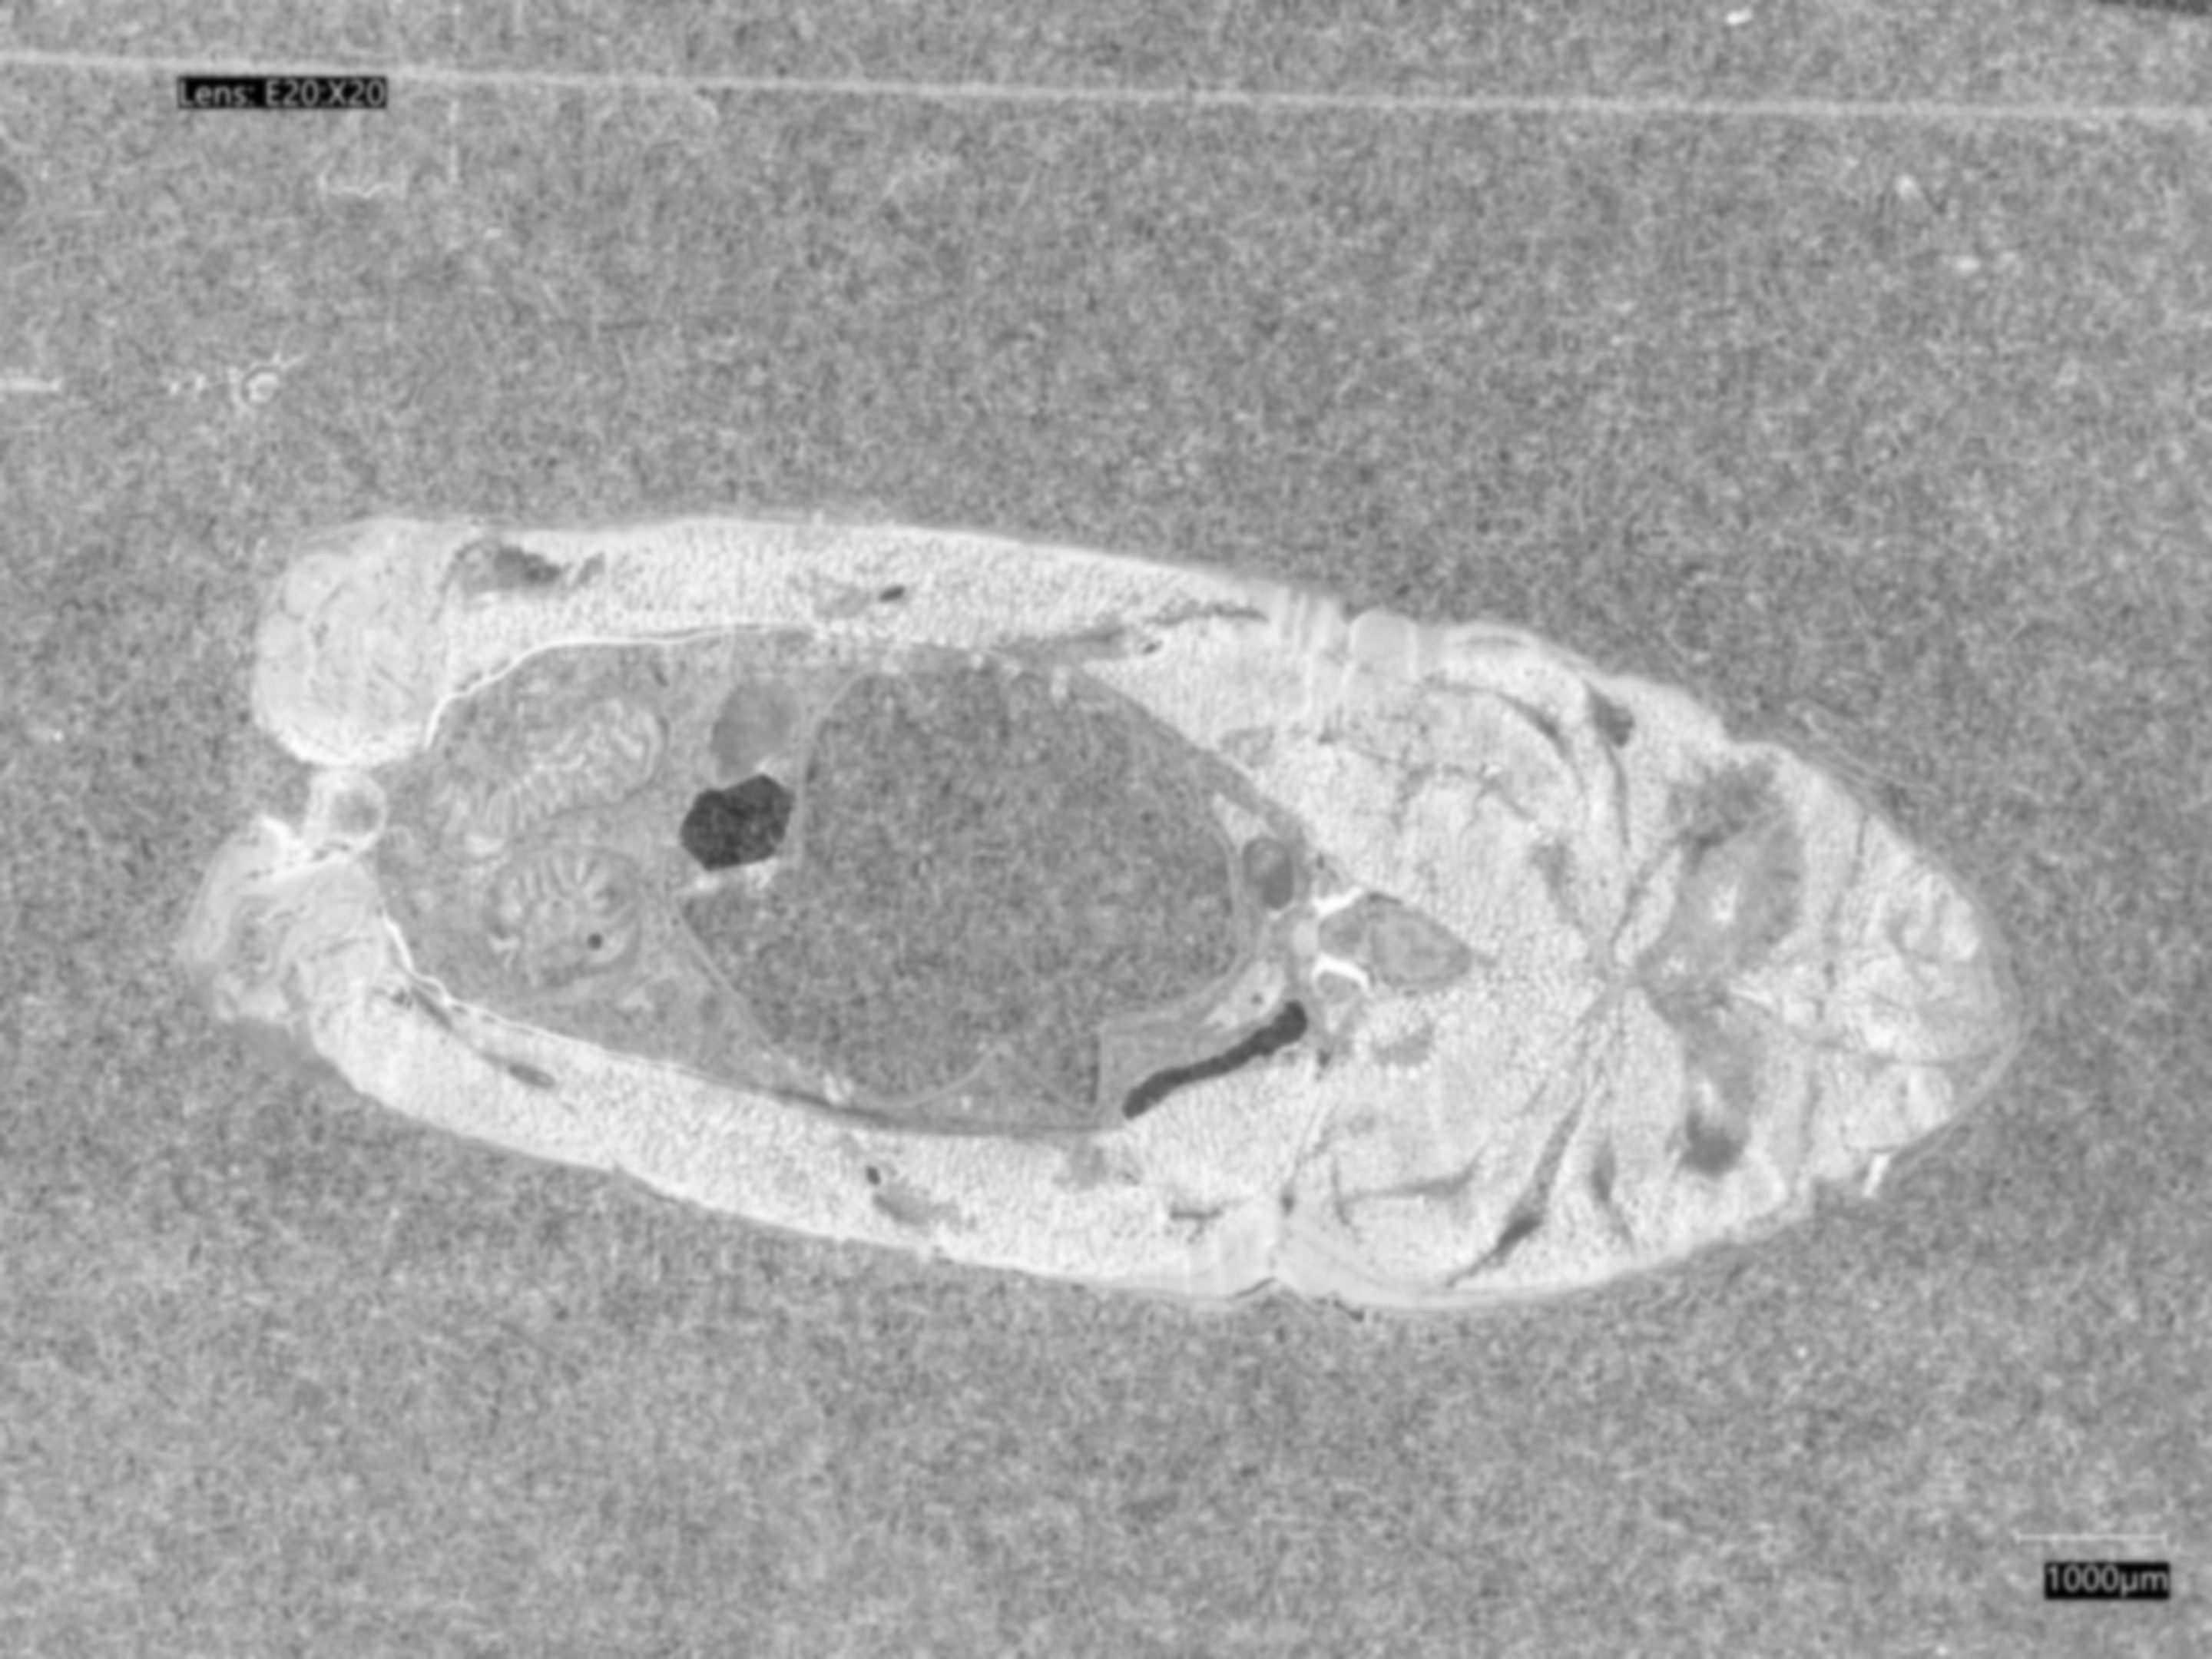
\includegraphics[width=\textwidth]{./fig/gausssian/blurred21.jpg}
        \caption{blurred k=21}
        \label{fig:blurred21}
    \end{minipage}
    \begin{minipage}{0.45\textwidth}
        \centering
        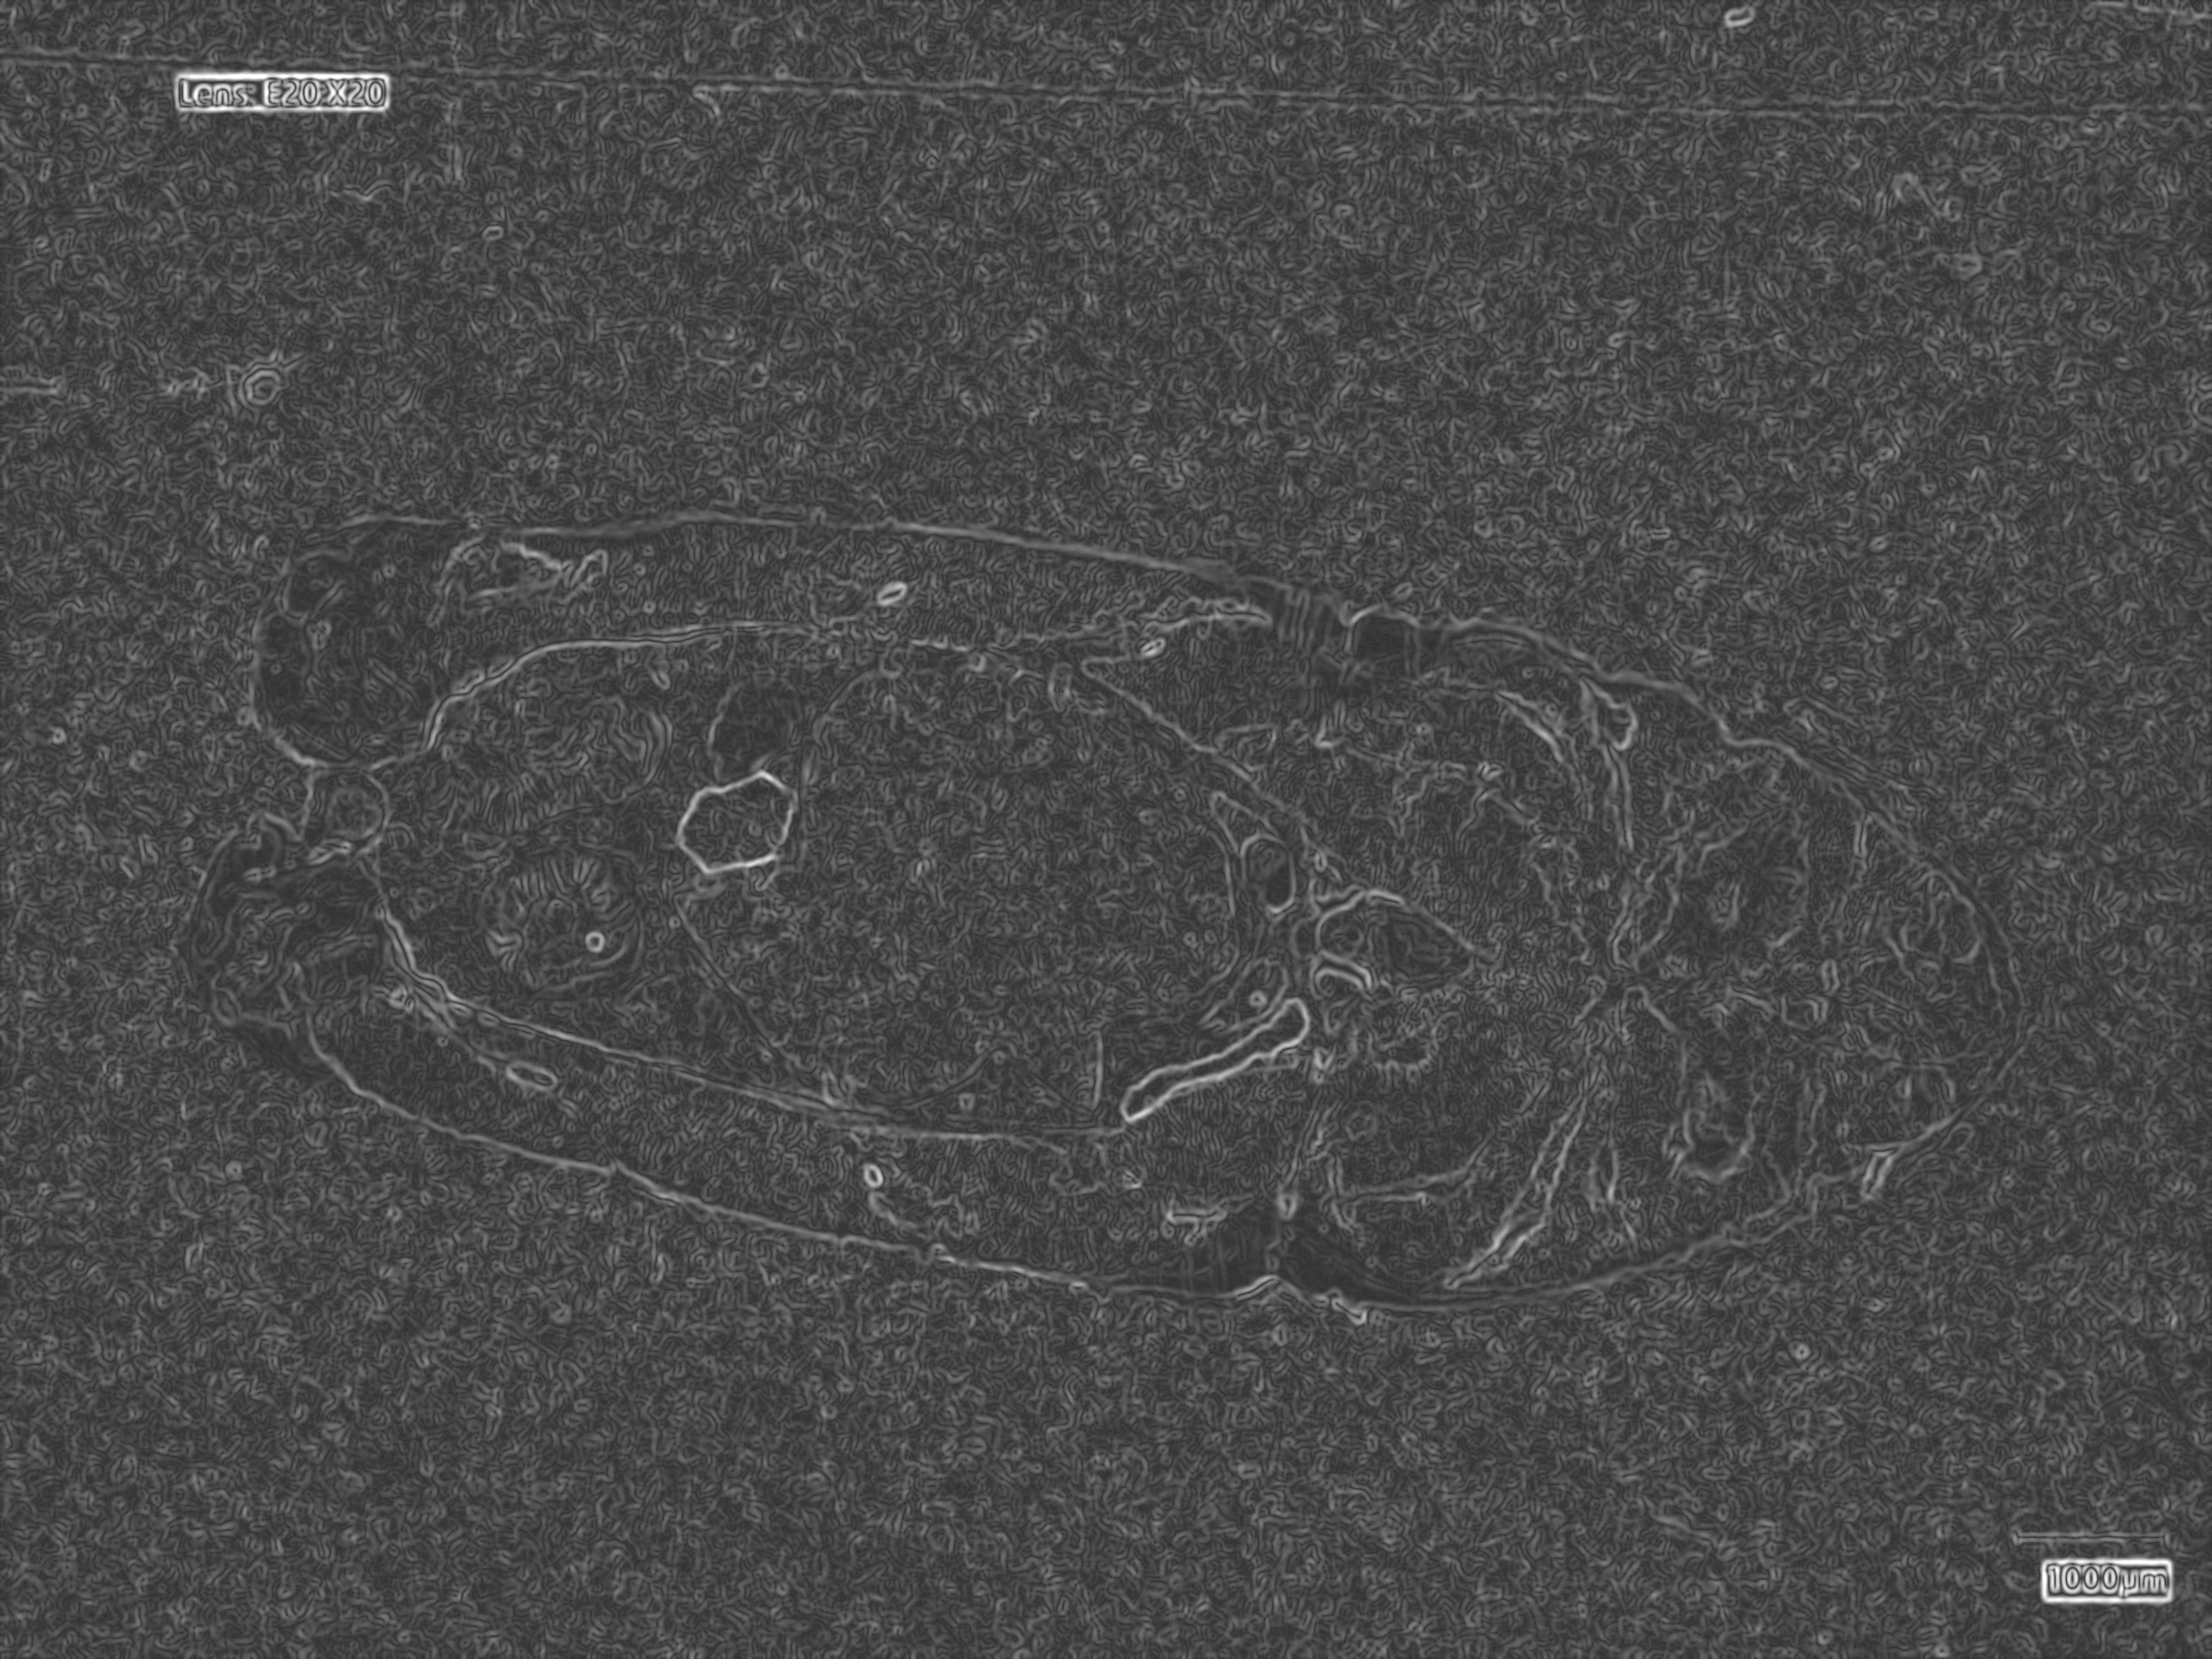
\includegraphics[width=\textwidth]{./fig/gausssian/sobel21.jpg}
        \caption{sobel k=21}
        \label{fig:sobel21}
    \end{minipage}
\end{figure}

\begin{figure}
    \centering
    \begin{minipage}{0.45\textwidth}
        \centering
        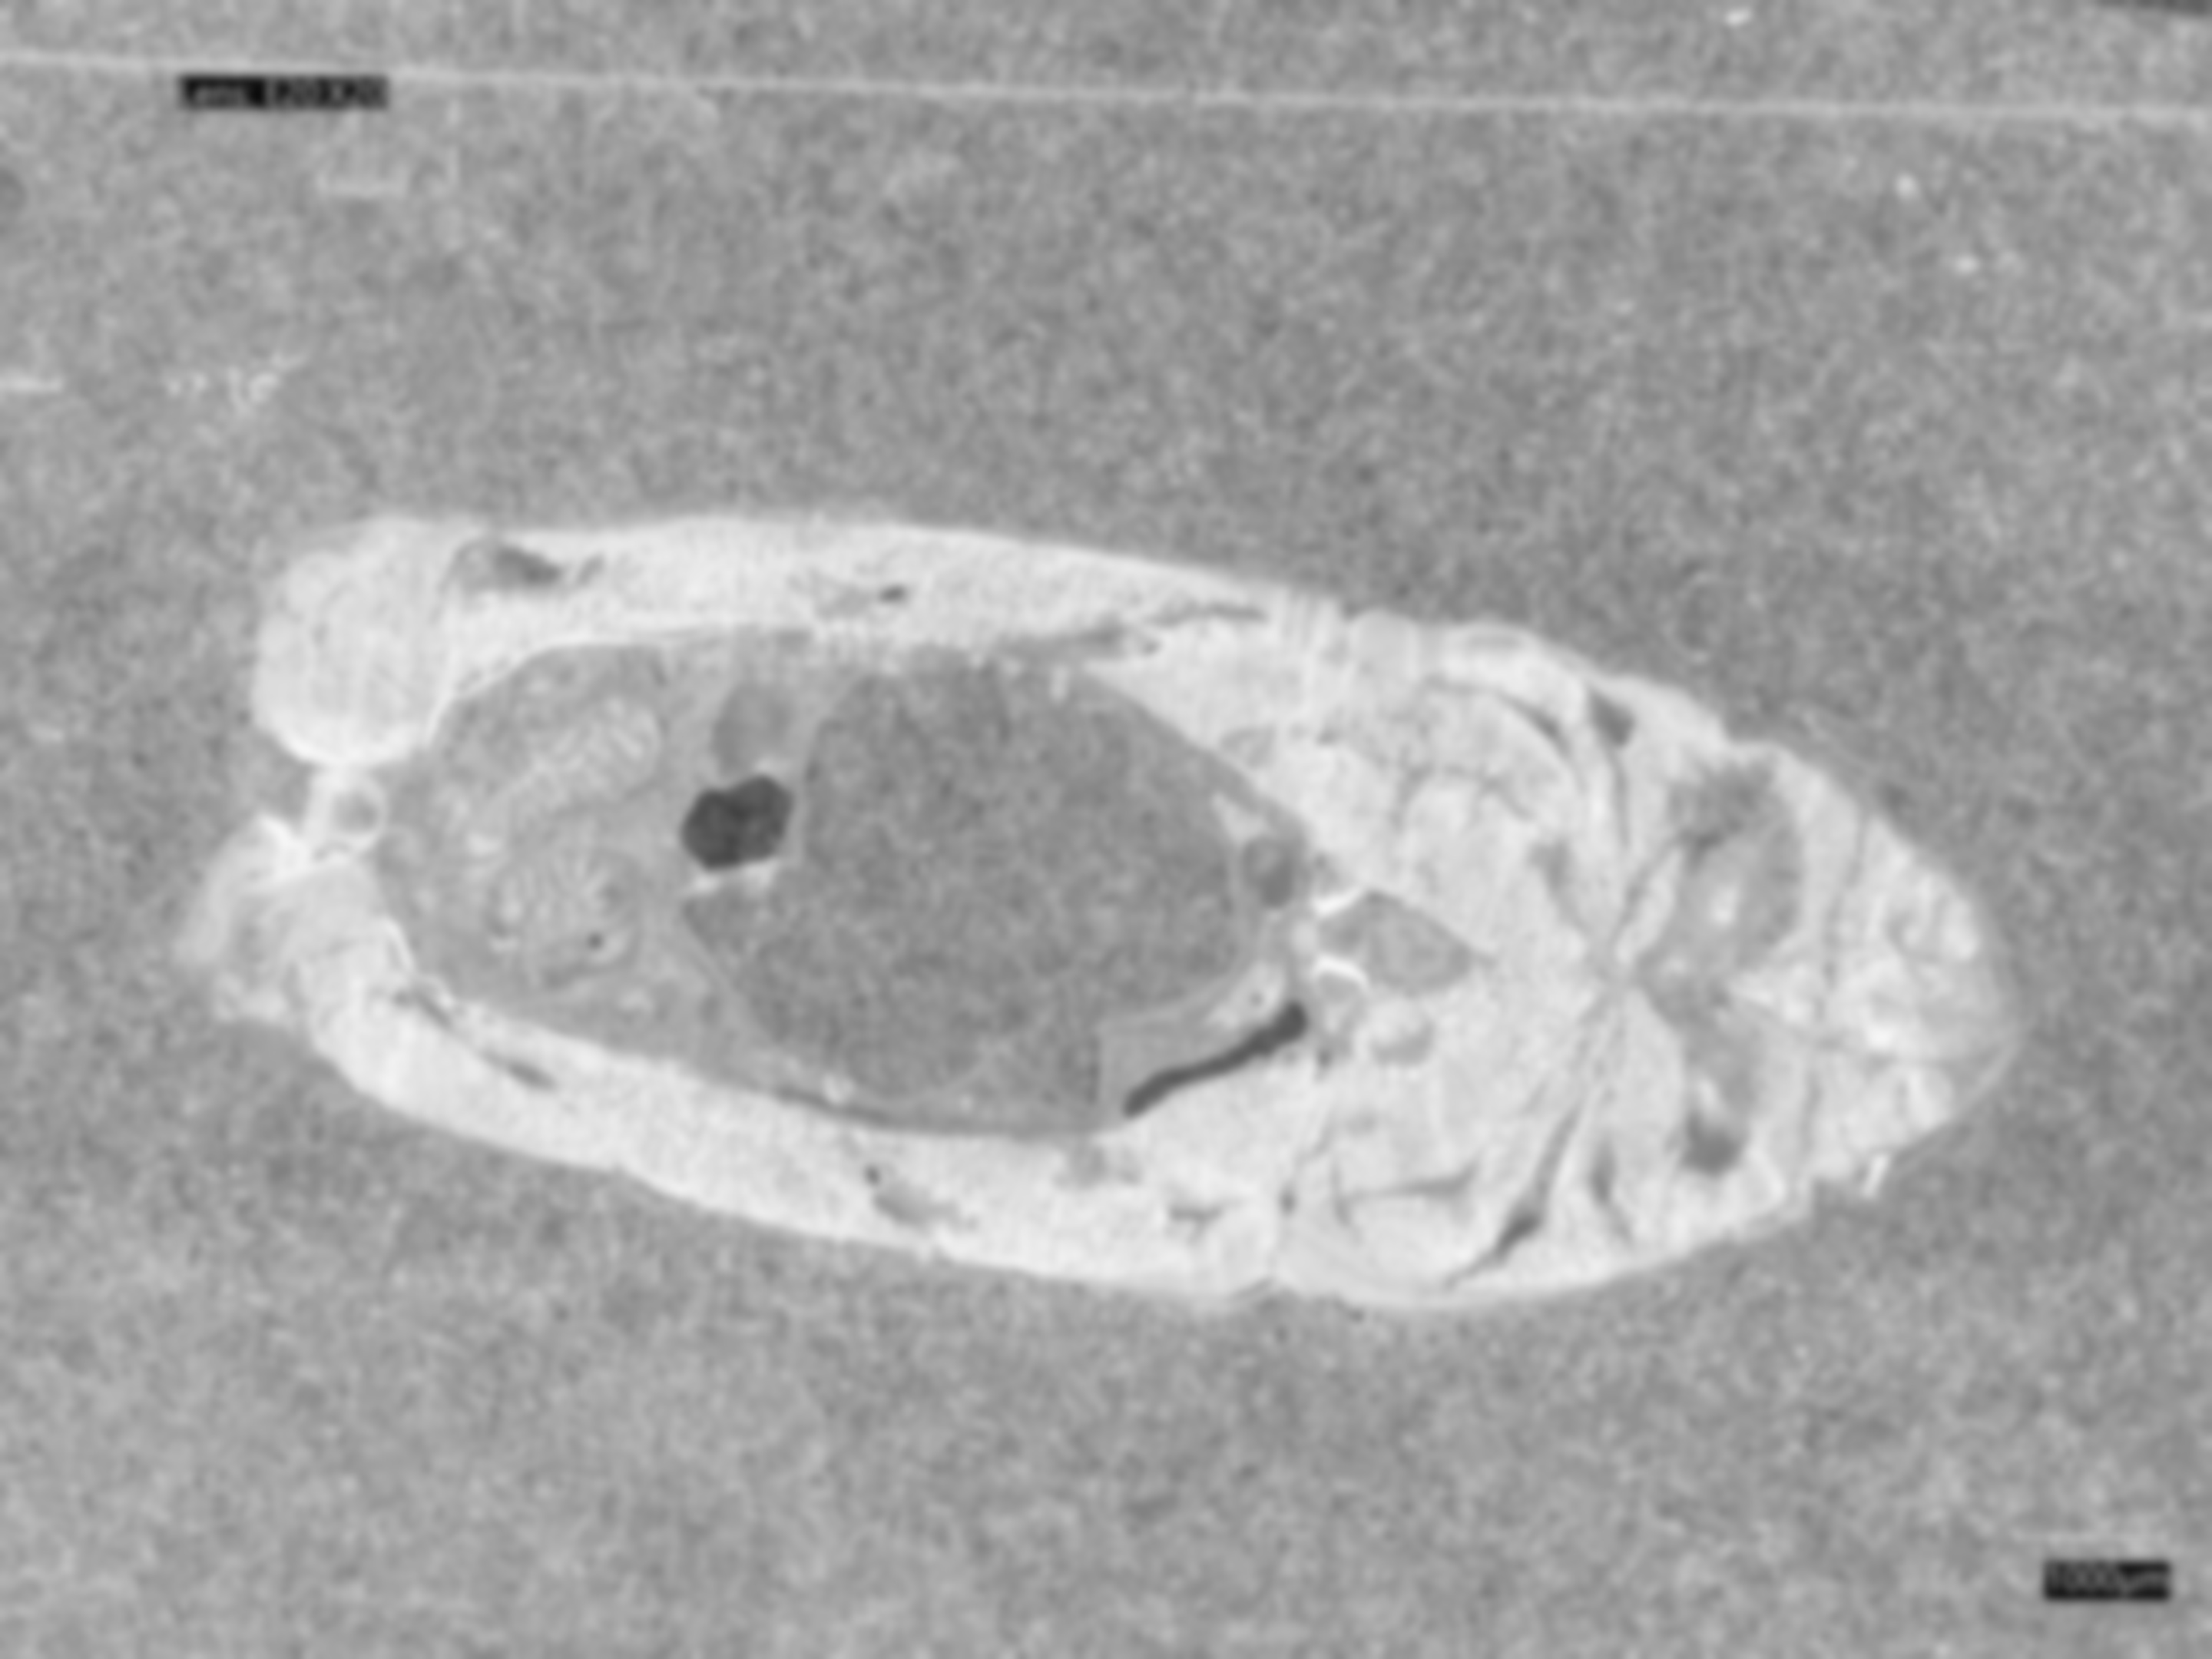
\includegraphics[width=\textwidth]{./fig/gausssian/blurred41.jpg}
        \caption{blurred k=41}
        \label{fig:blurred41}
    \end{minipage}
    \begin{minipage}{0.45\textwidth}
        \centering
        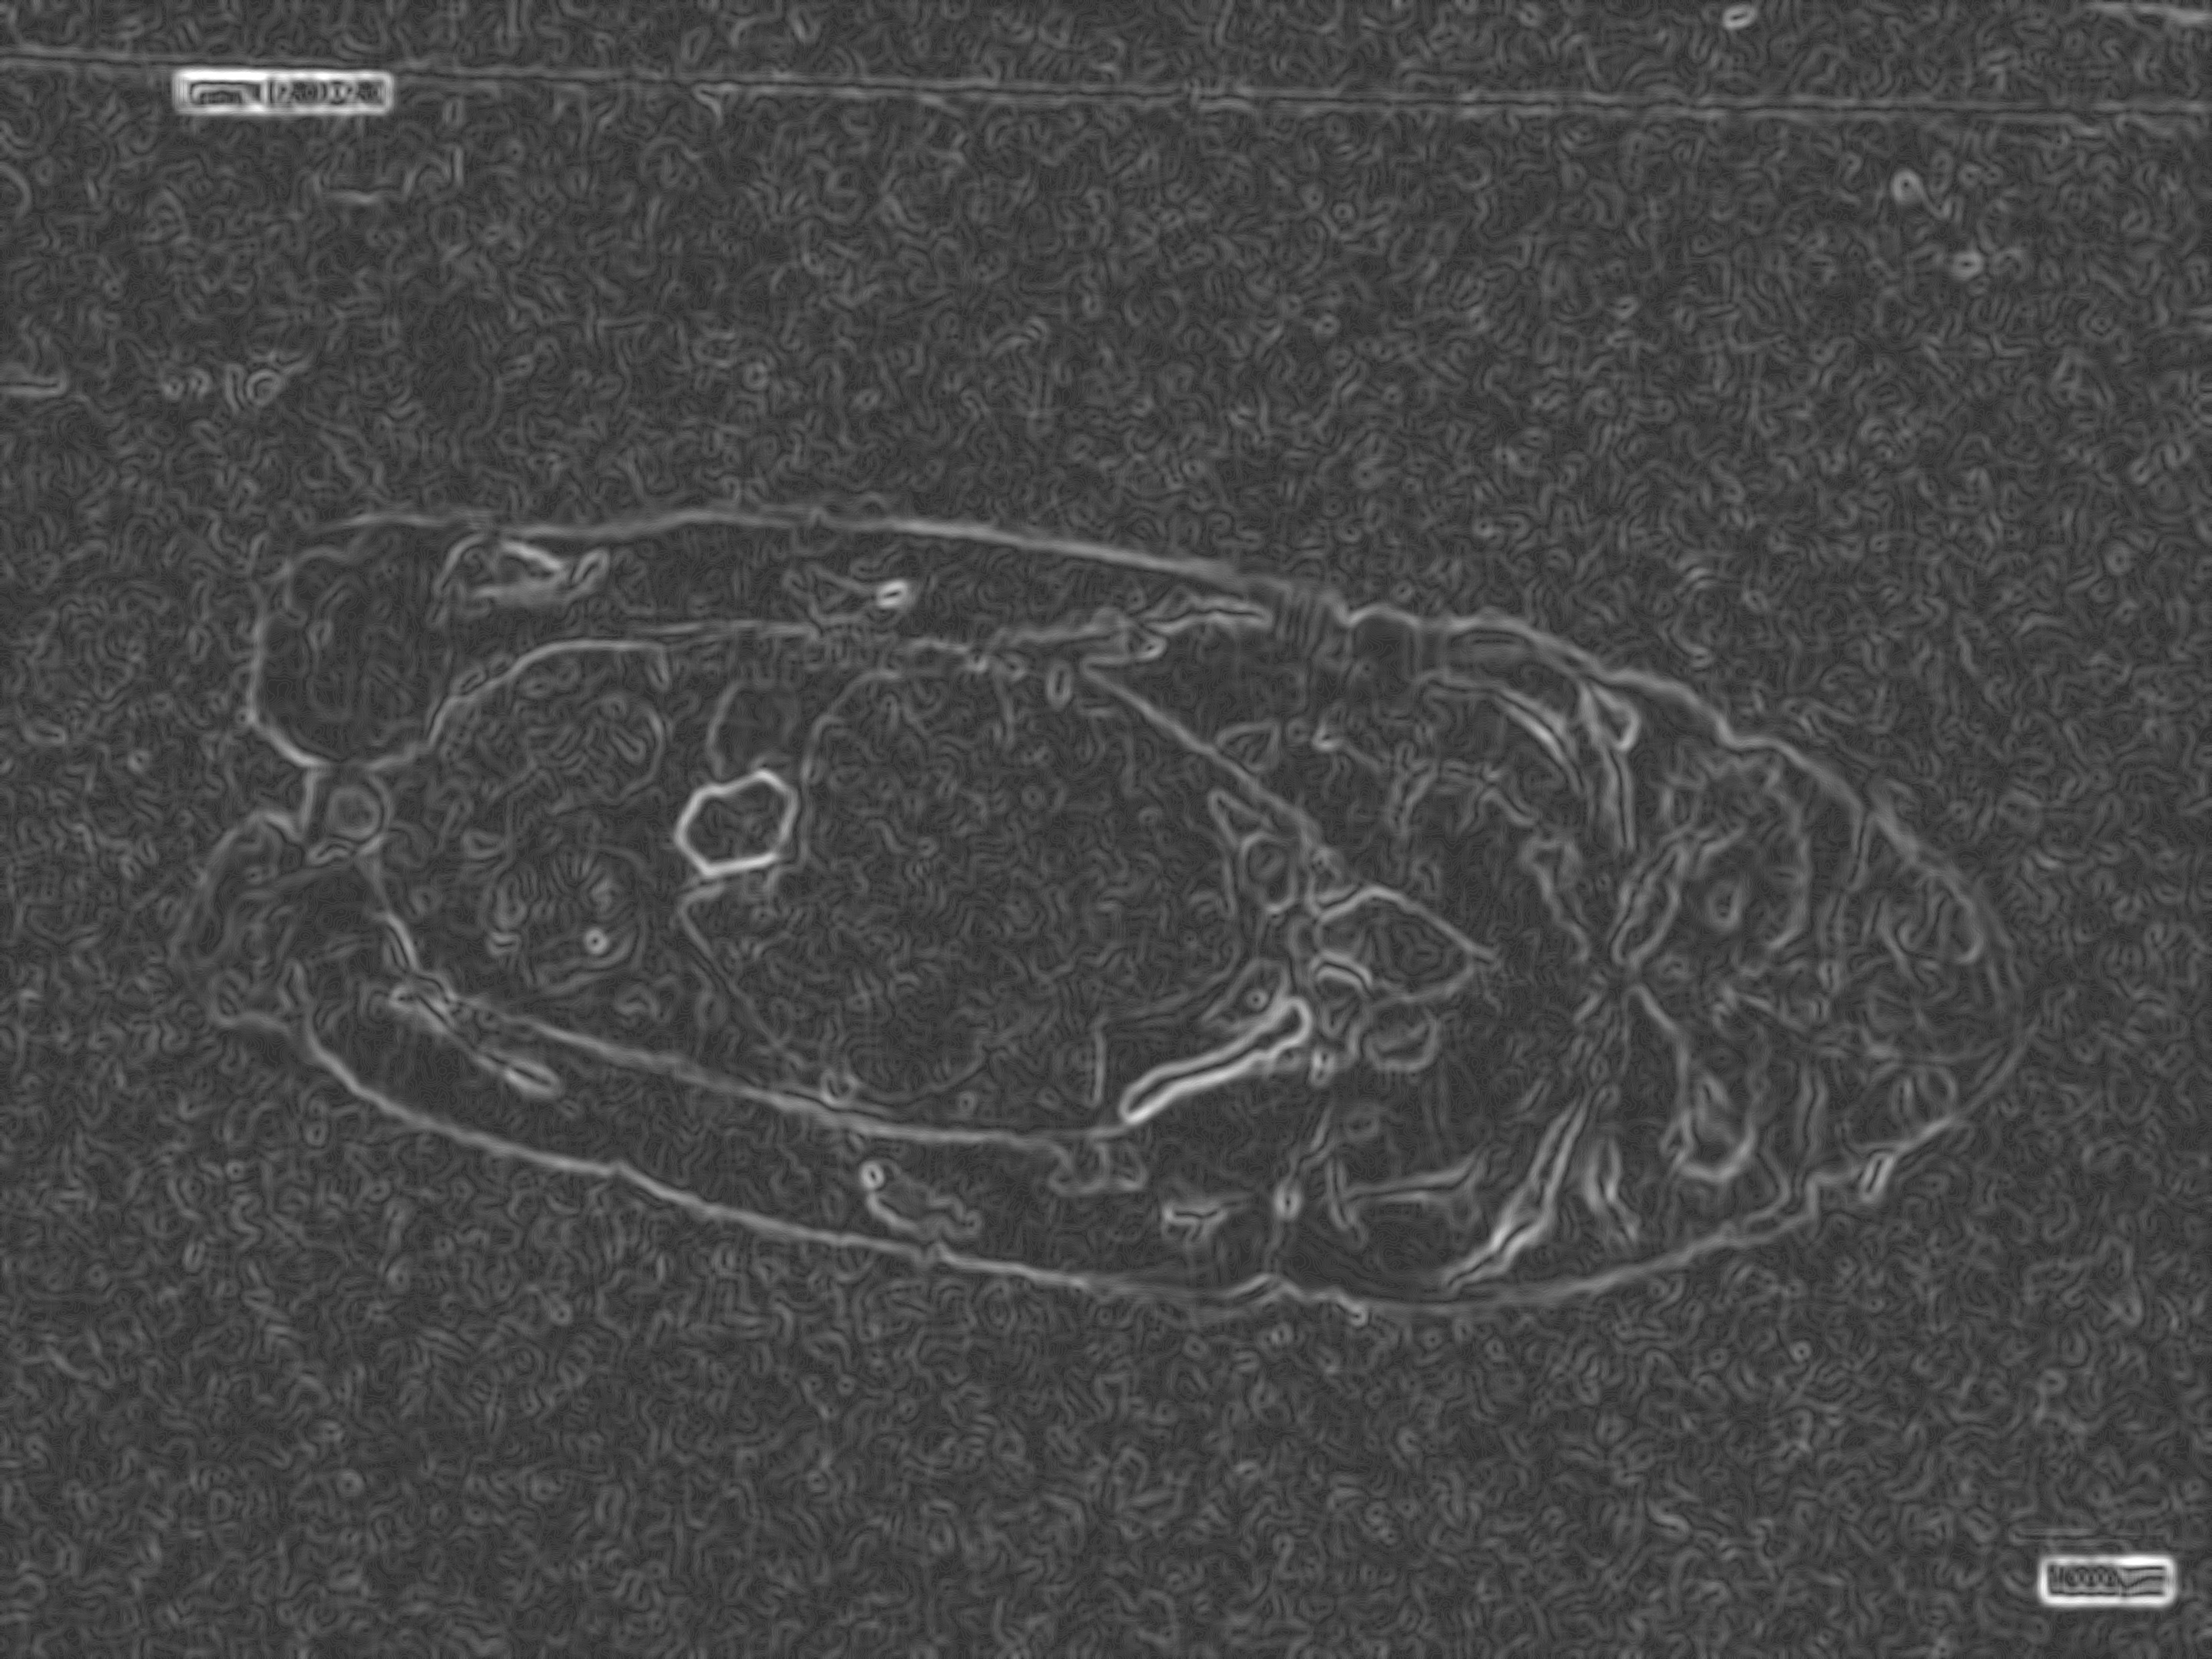
\includegraphics[width=\textwidth]{./fig/gausssian/sobel41.jpg}
        \caption{sobel k=41}
        \label{fig:sobel41}
    \end{minipage}
\end{figure}

\begin{figure}
    \centering
    \begin{minipage}{0.45\textwidth}
        \centering
        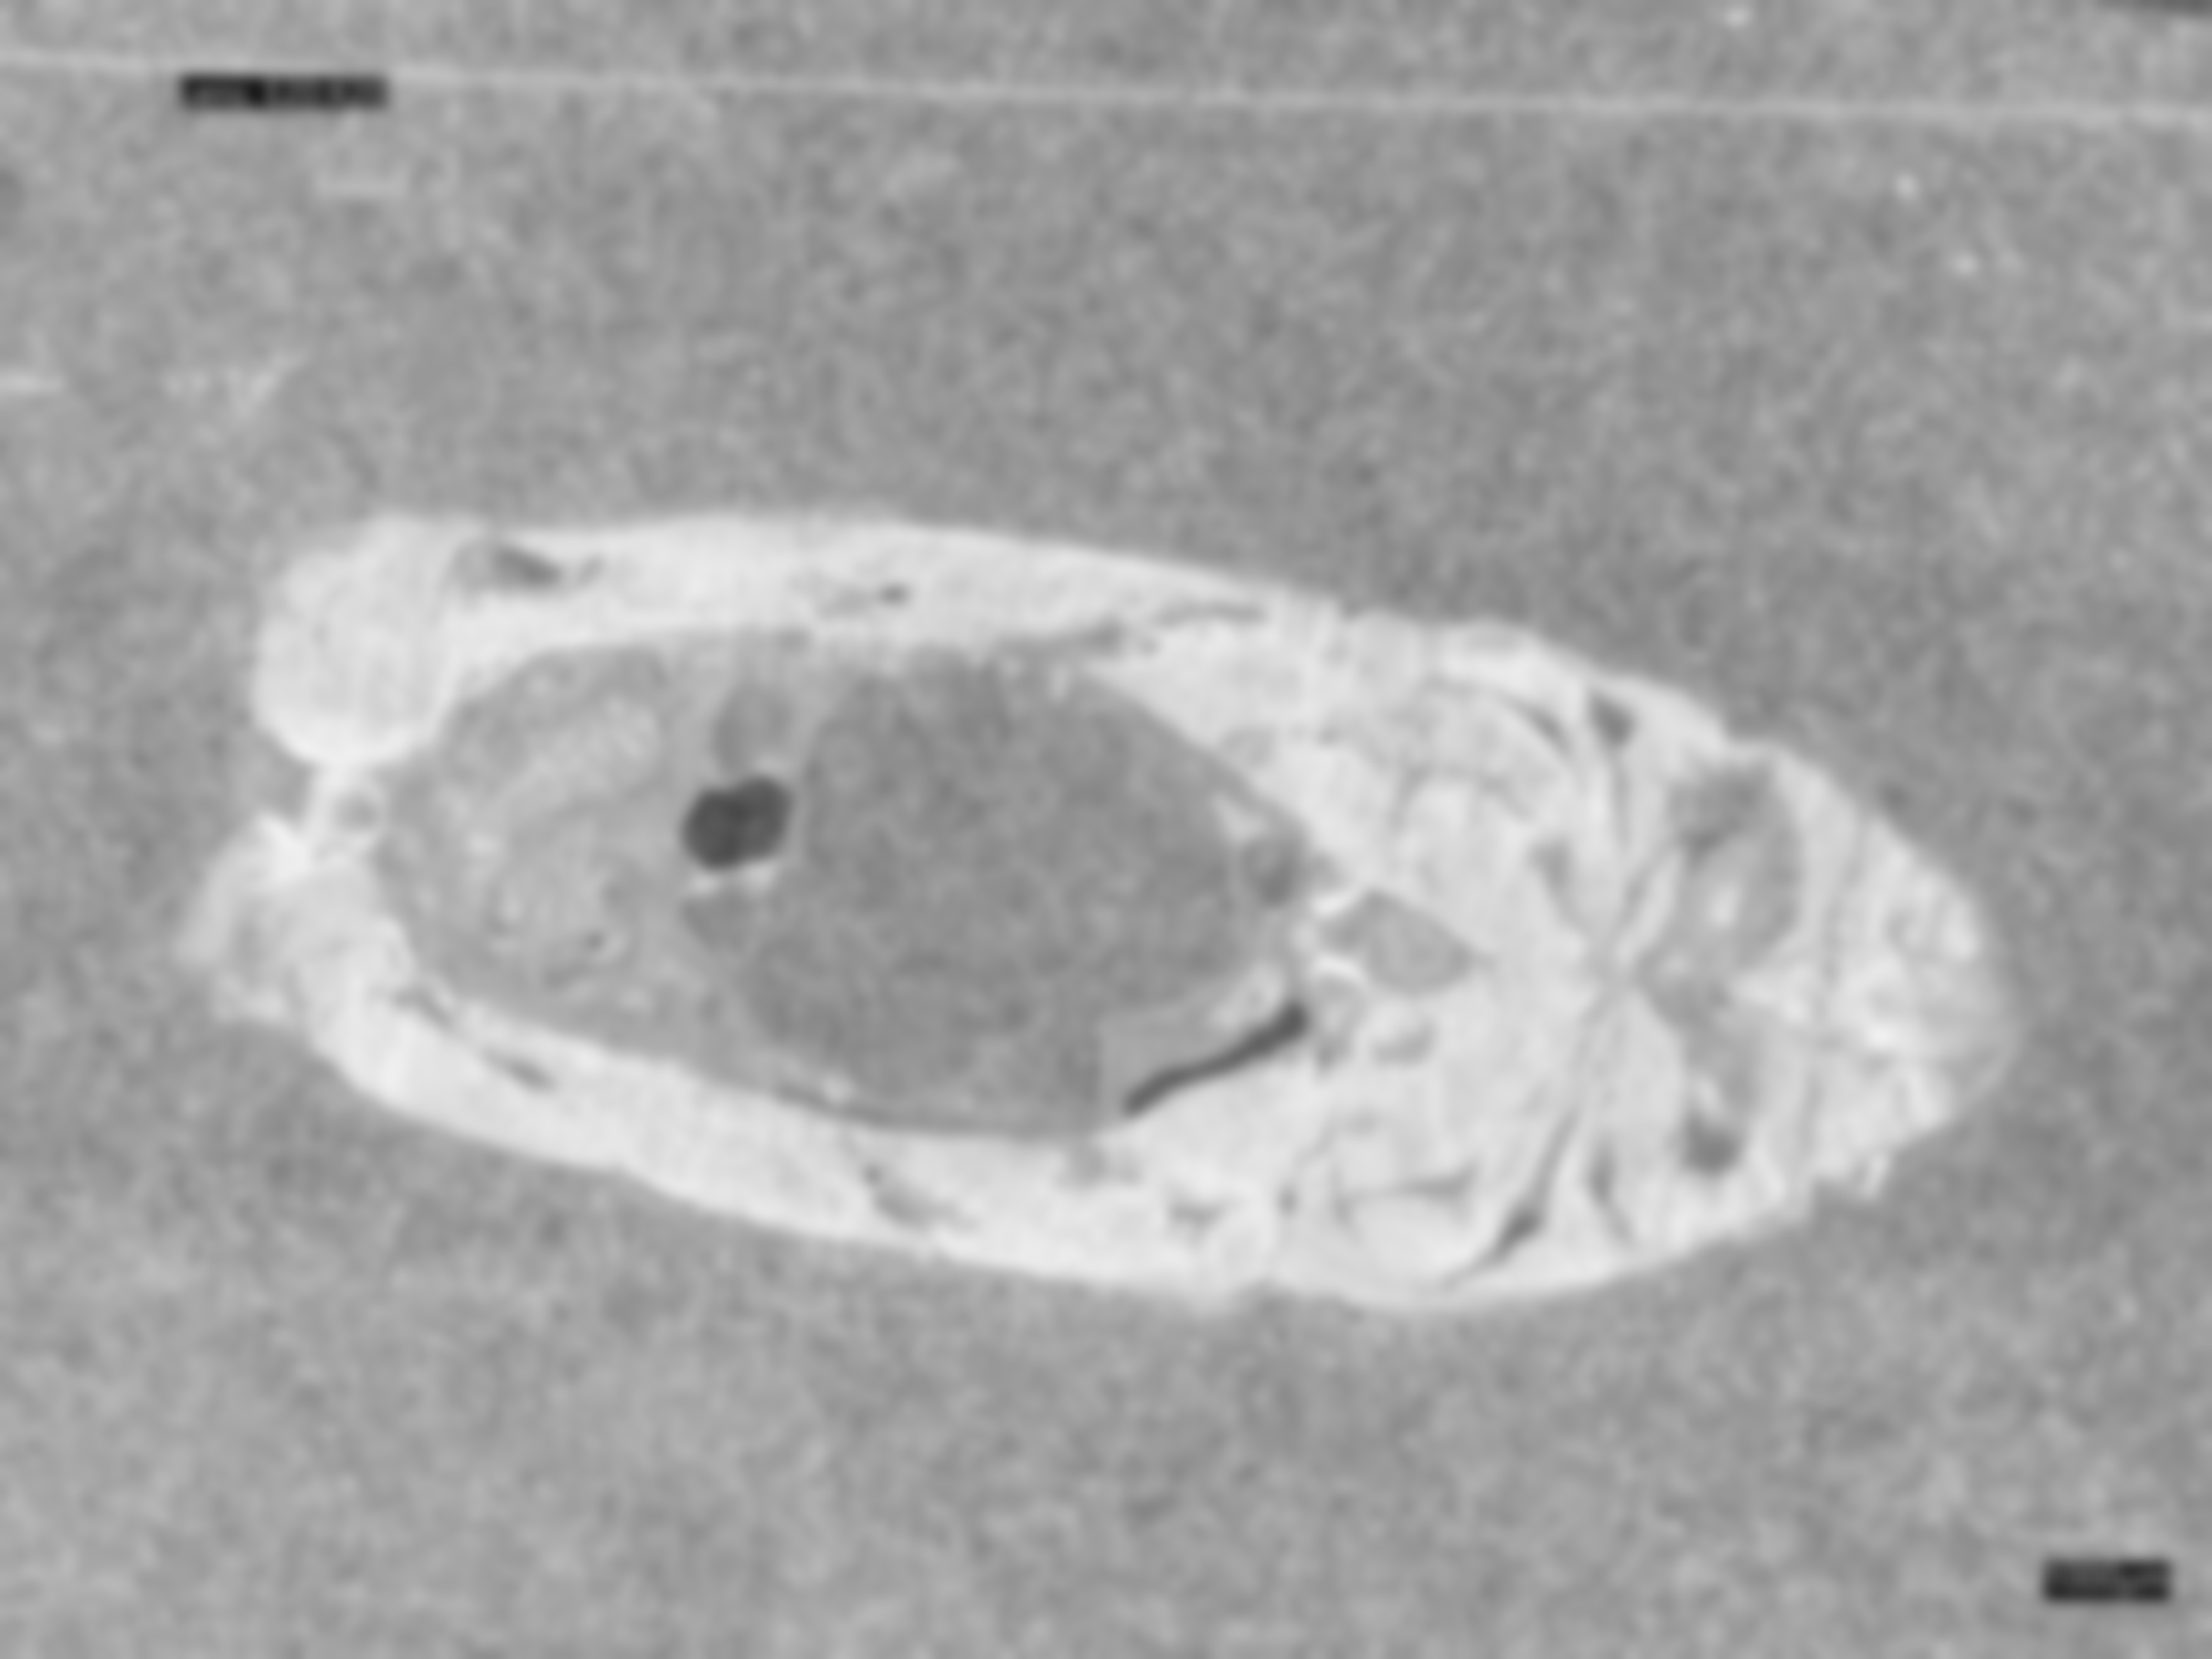
\includegraphics[width=\textwidth]{./fig/gausssian/blurred61.jpg}
        \caption{blurred k=61}
        \label{fig:blurred61}
    \end{minipage}
    \begin{minipage}{0.45\textwidth}
        \centering
        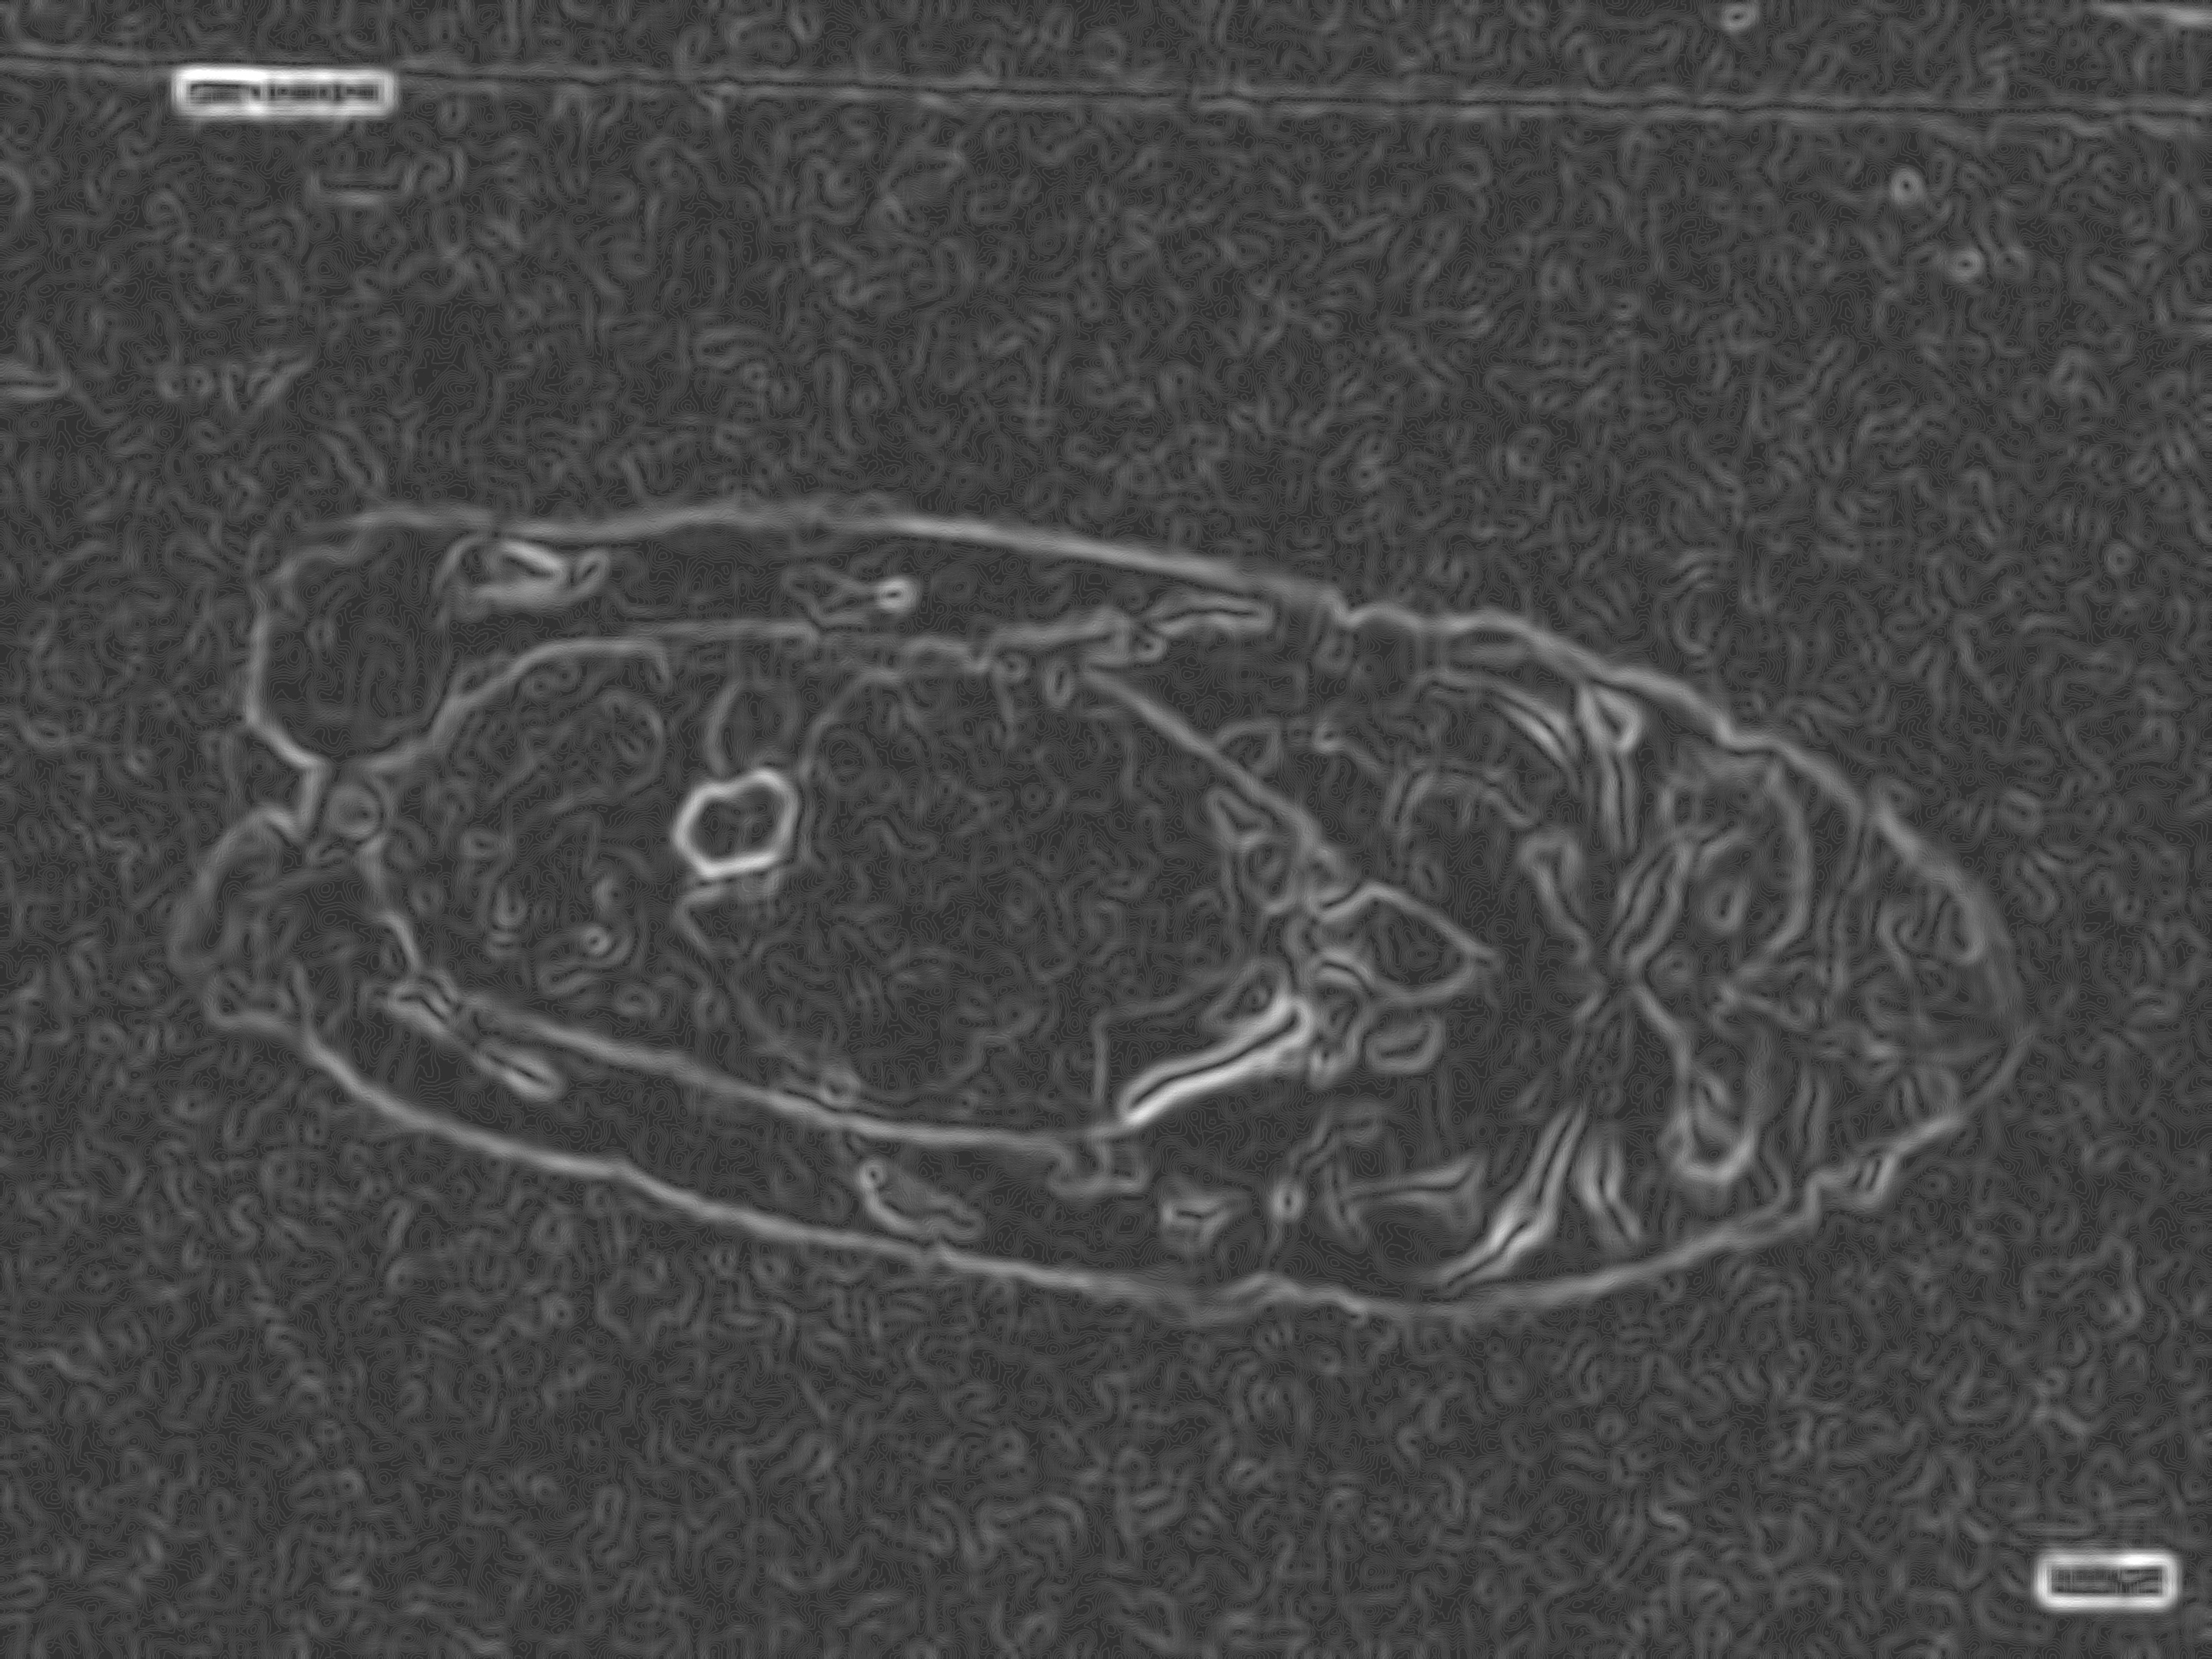
\includegraphics[width=\textwidth]{./fig/gausssian/sobel61.jpg}
        \caption{sobel k=61}
        \label{fig:sobel61}
    \end{minipage}
\end{figure}

\begin{figure}
    \centering
    \begin{minipage}{0.45\textwidth}
        \centering
        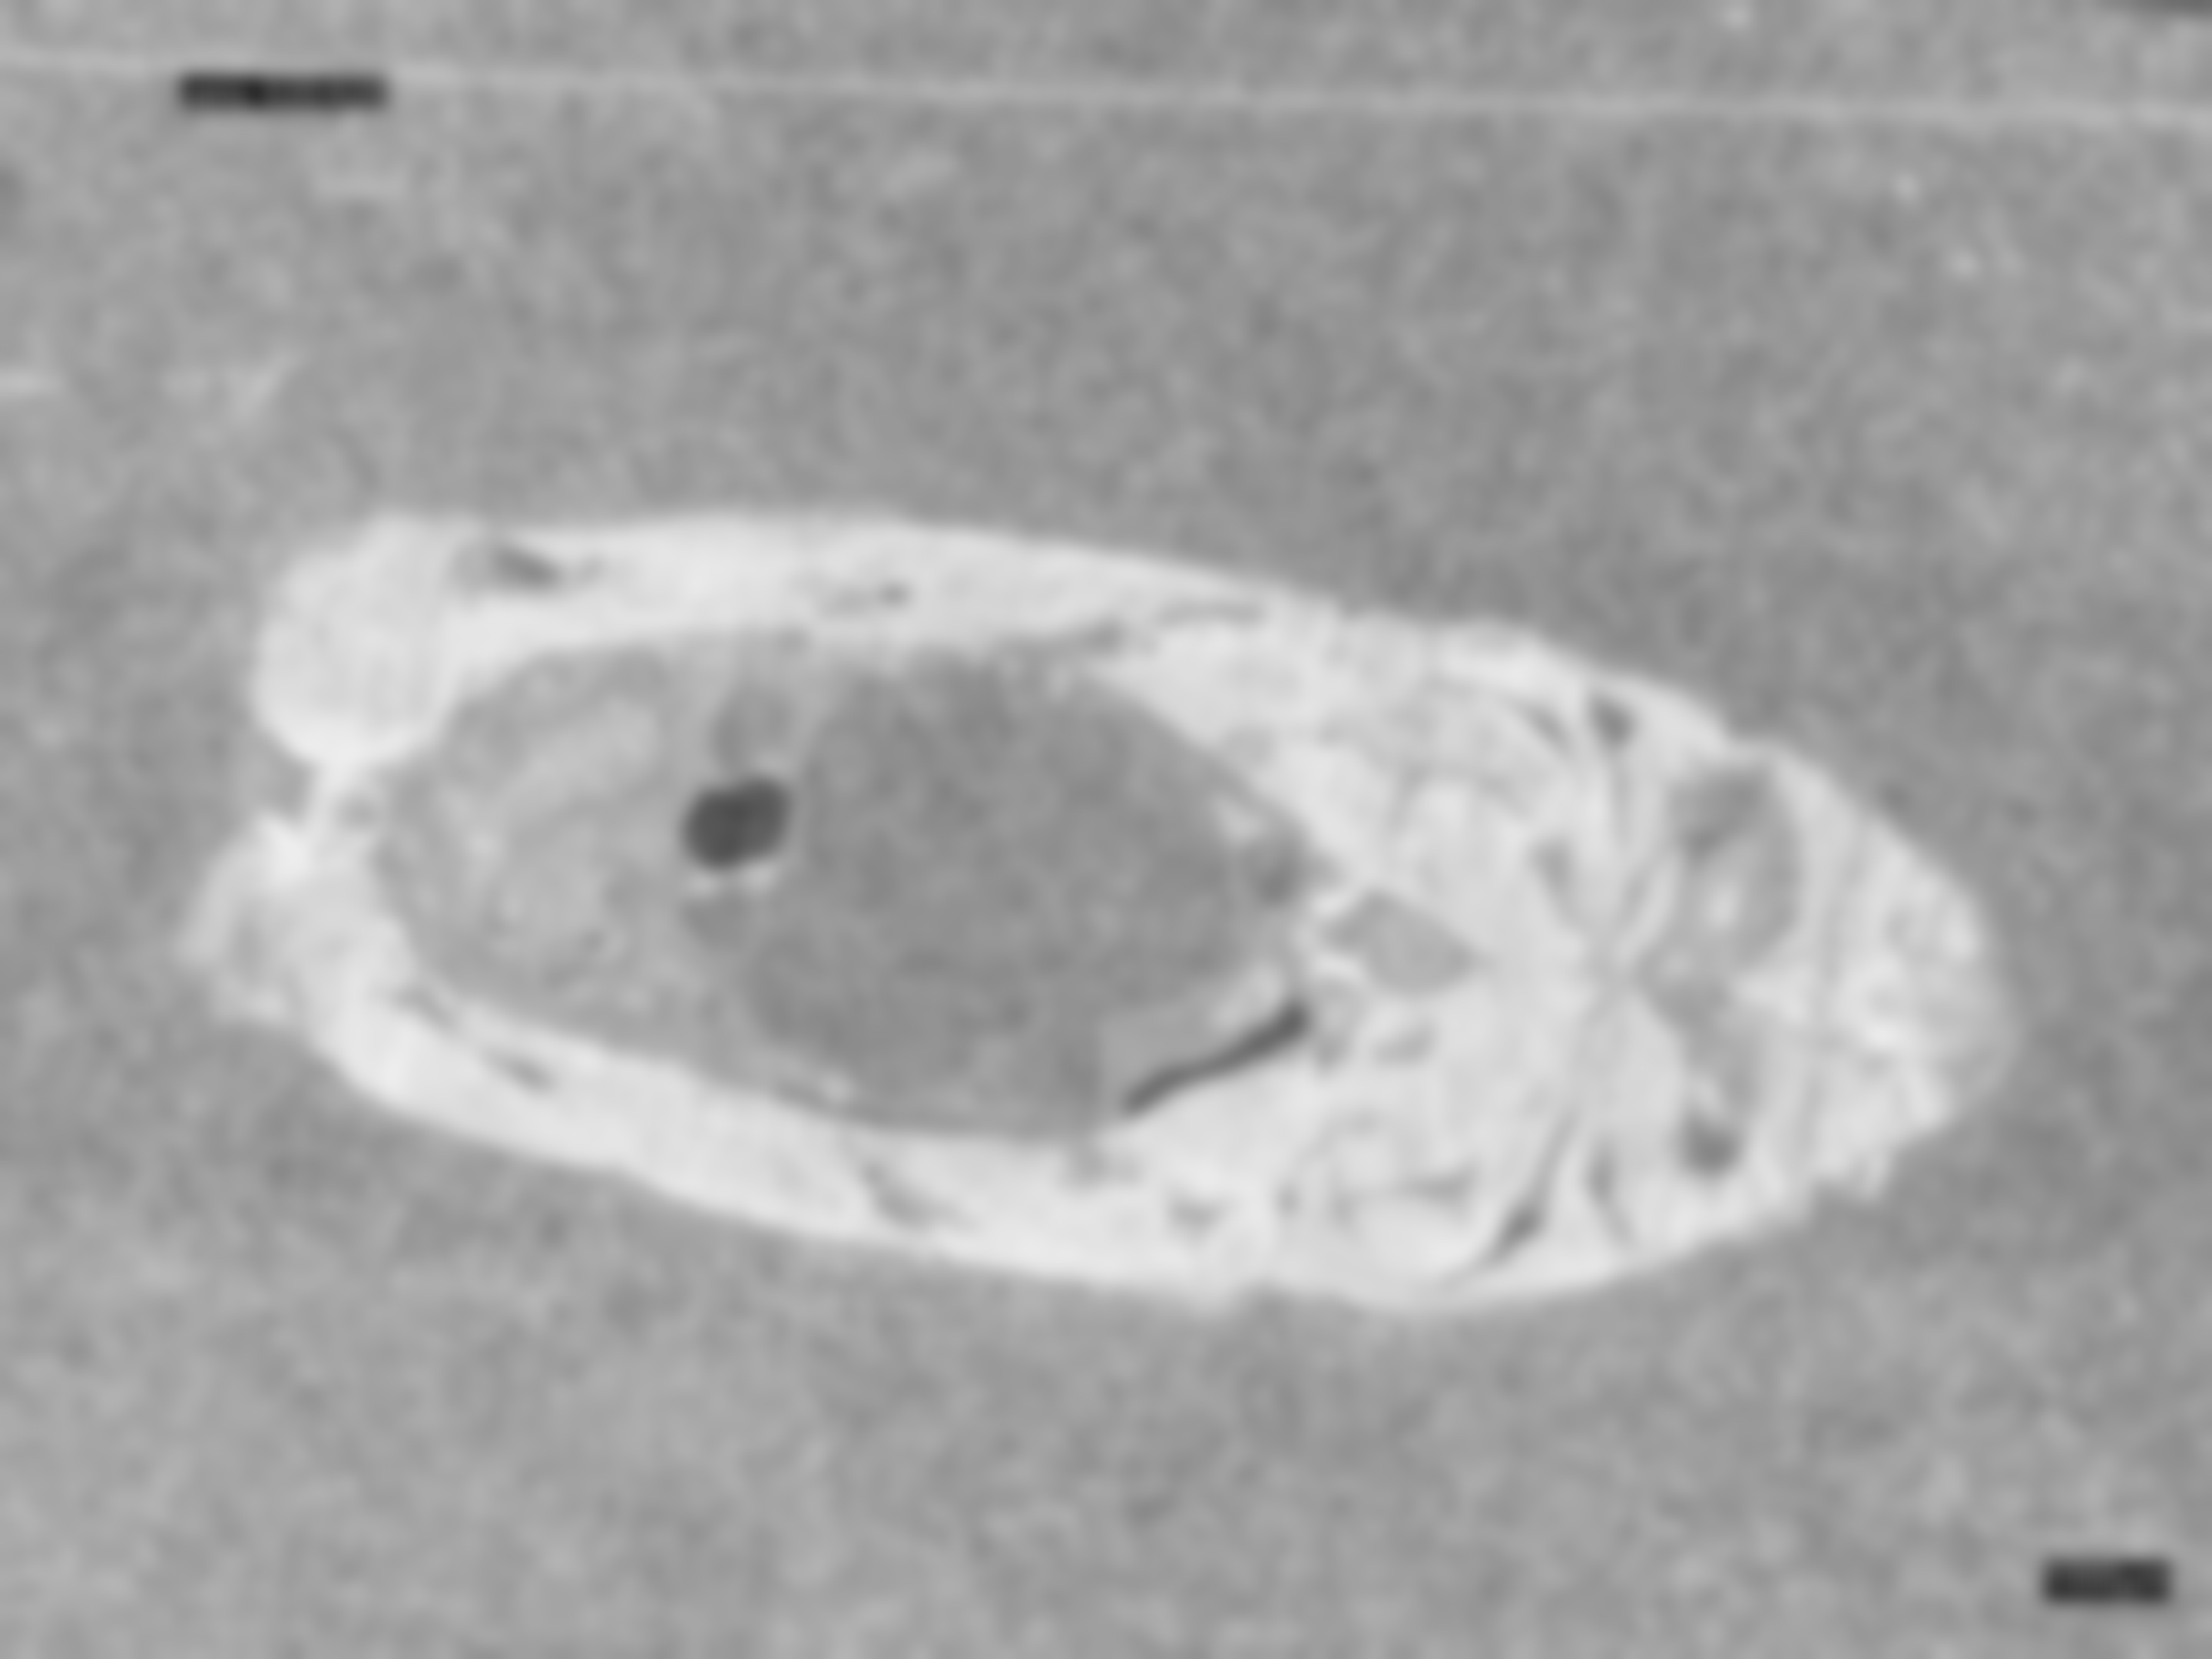
\includegraphics[width=\textwidth]{./fig/gausssian/blurred81.jpg}
        \caption{blurred k=81}
        \label{fig:blurred81}
    \end{minipage}
    \begin{minipage}{0.45\textwidth}
        \centering
        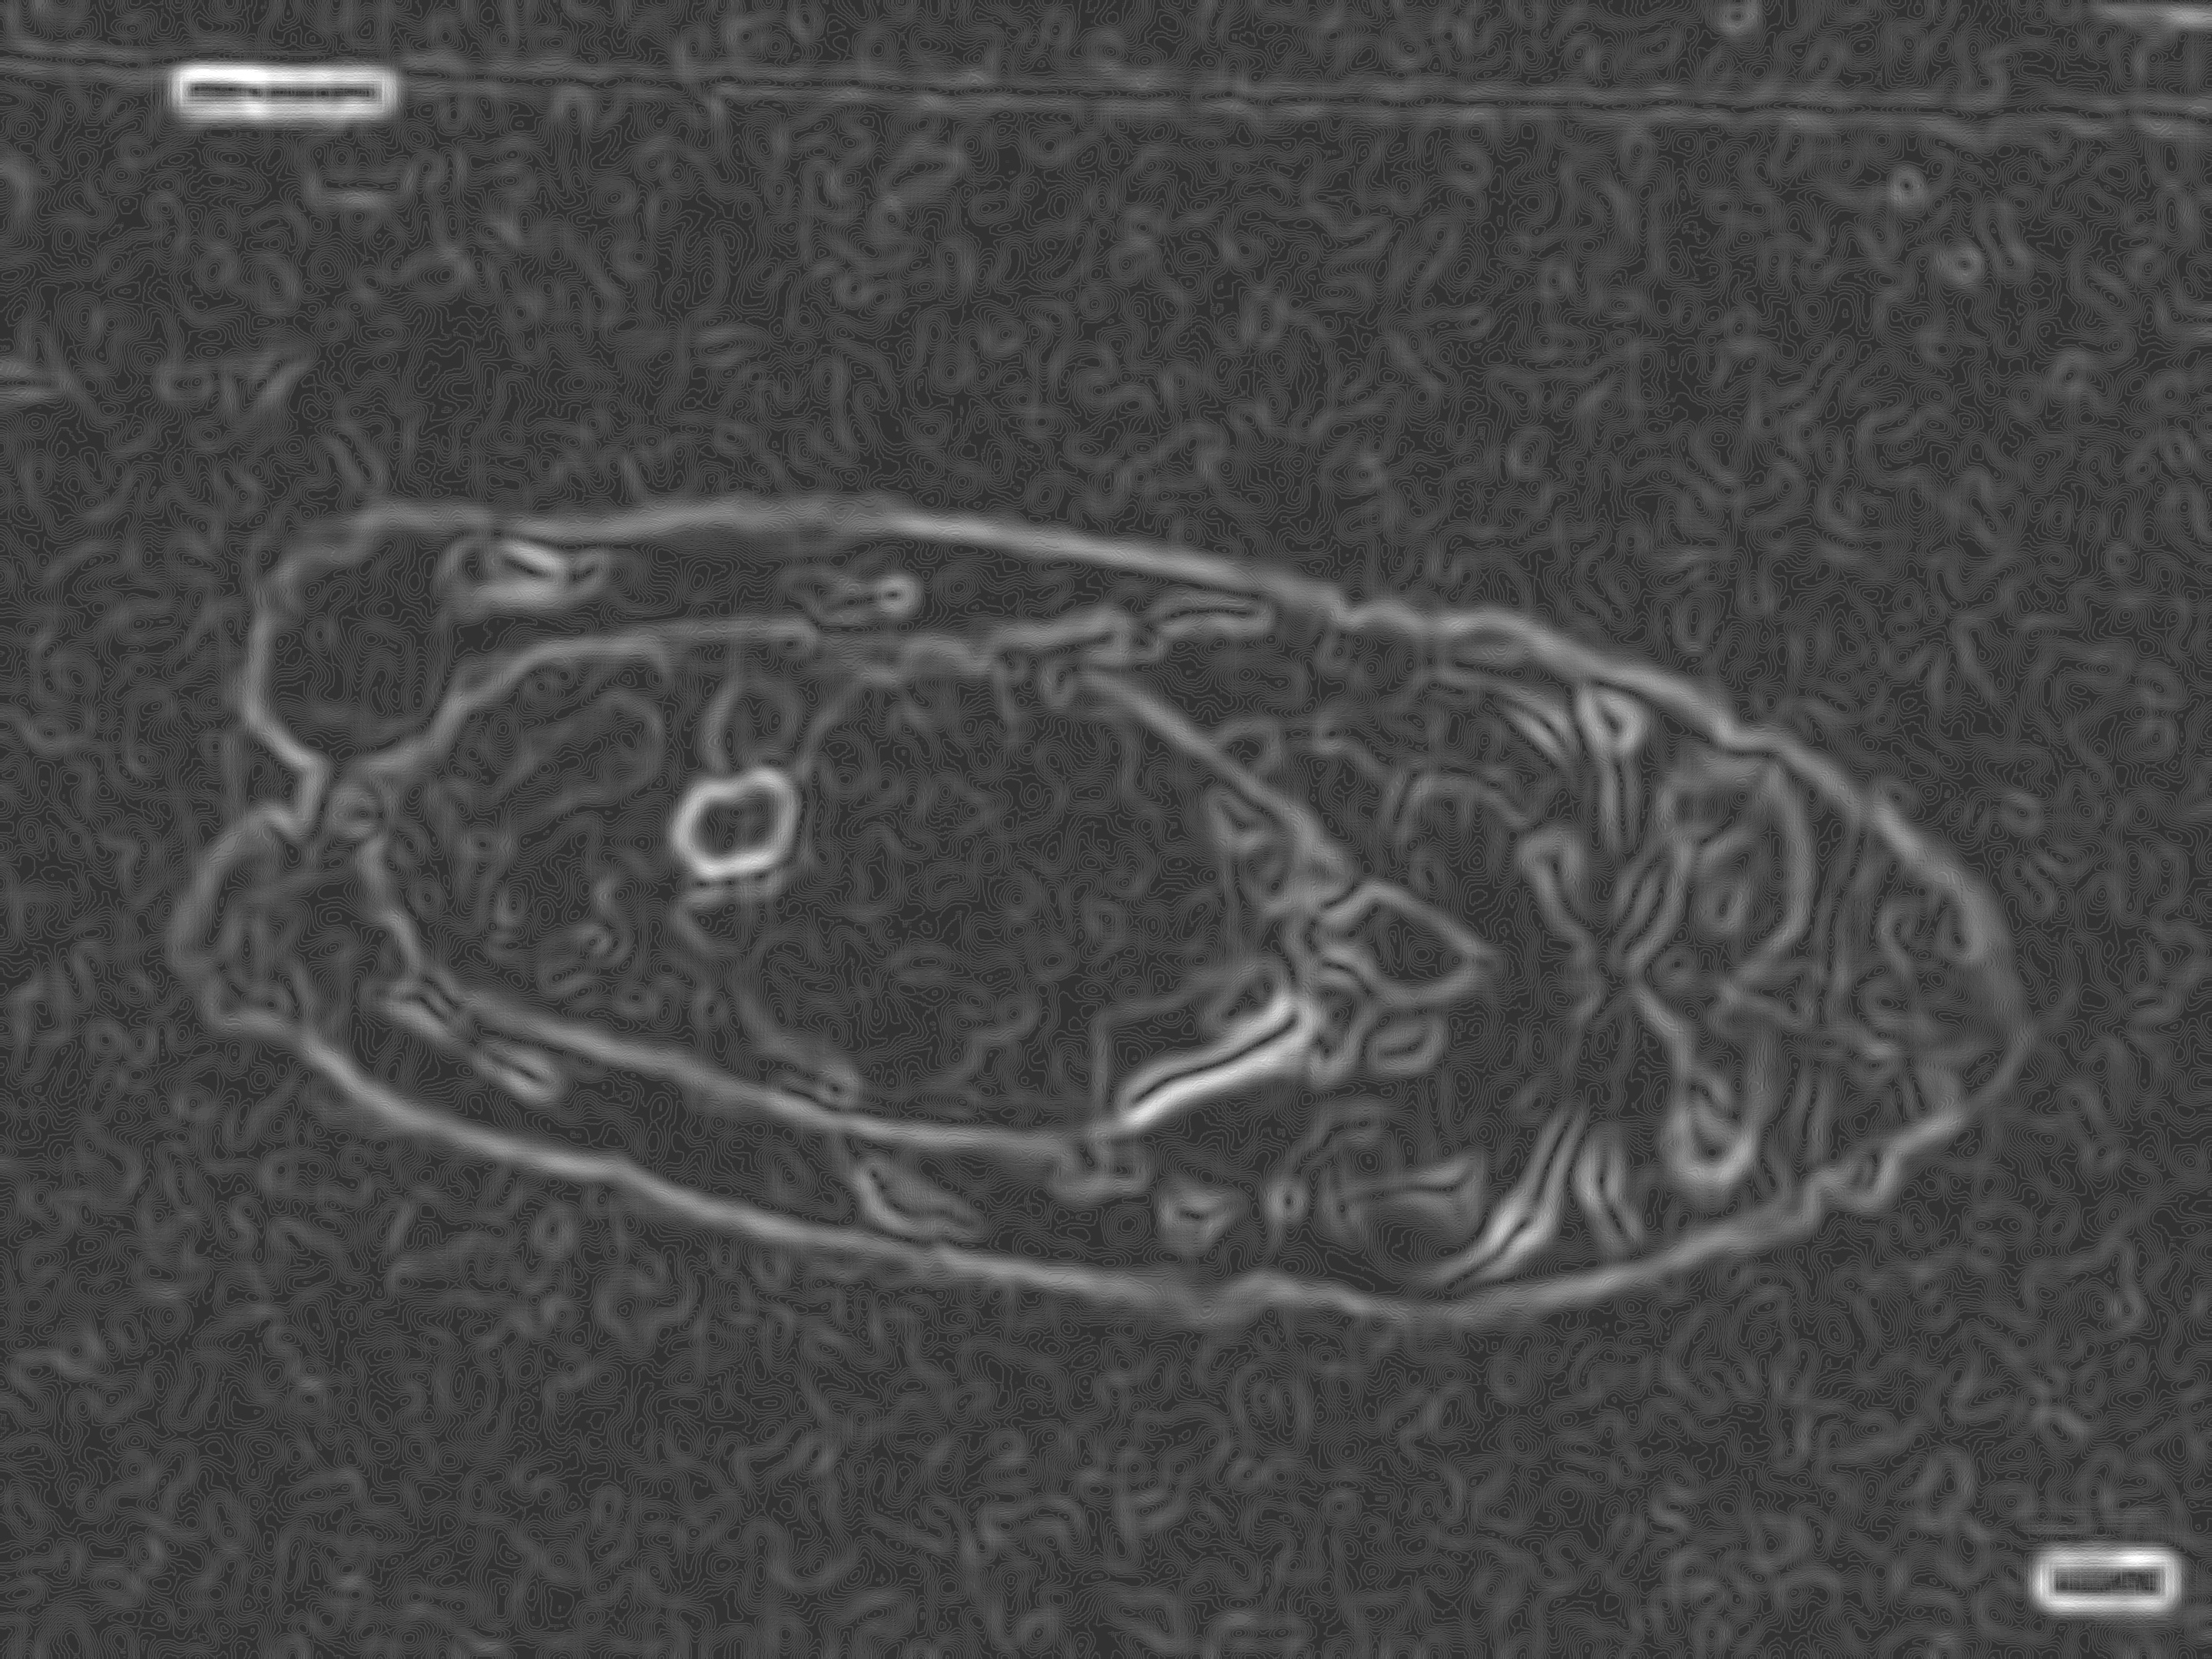
\includegraphics[width=\textwidth]{./fig/gausssian/sobel81.jpg}
        \caption{sobel k=81}
        \label{fig:sobel81}
    \end{minipage}
\end{figure}

从\autoref{fig:blurred21}到\autoref{fig:blurred81}可以看到,随着高斯模糊核的增大,图像的细节逐渐模糊,边缘也逐渐变得模糊。从\autoref{fig:sobel21}到\autoref{fig:sobel81}可以看到,随着高斯模糊核的增大,边缘检测的效果逐渐减弱,边缘变得不明显。考虑到图像边缘的清晰度和底噪的对比,我们选择高斯模糊核为61。


以下是在高斯模糊(k=61)后使用python的opencv库执行laplacian算子的结果。

\begin{figure}
    \centering
    \begin{minipage}{0.45\textwidth}
        \centering
        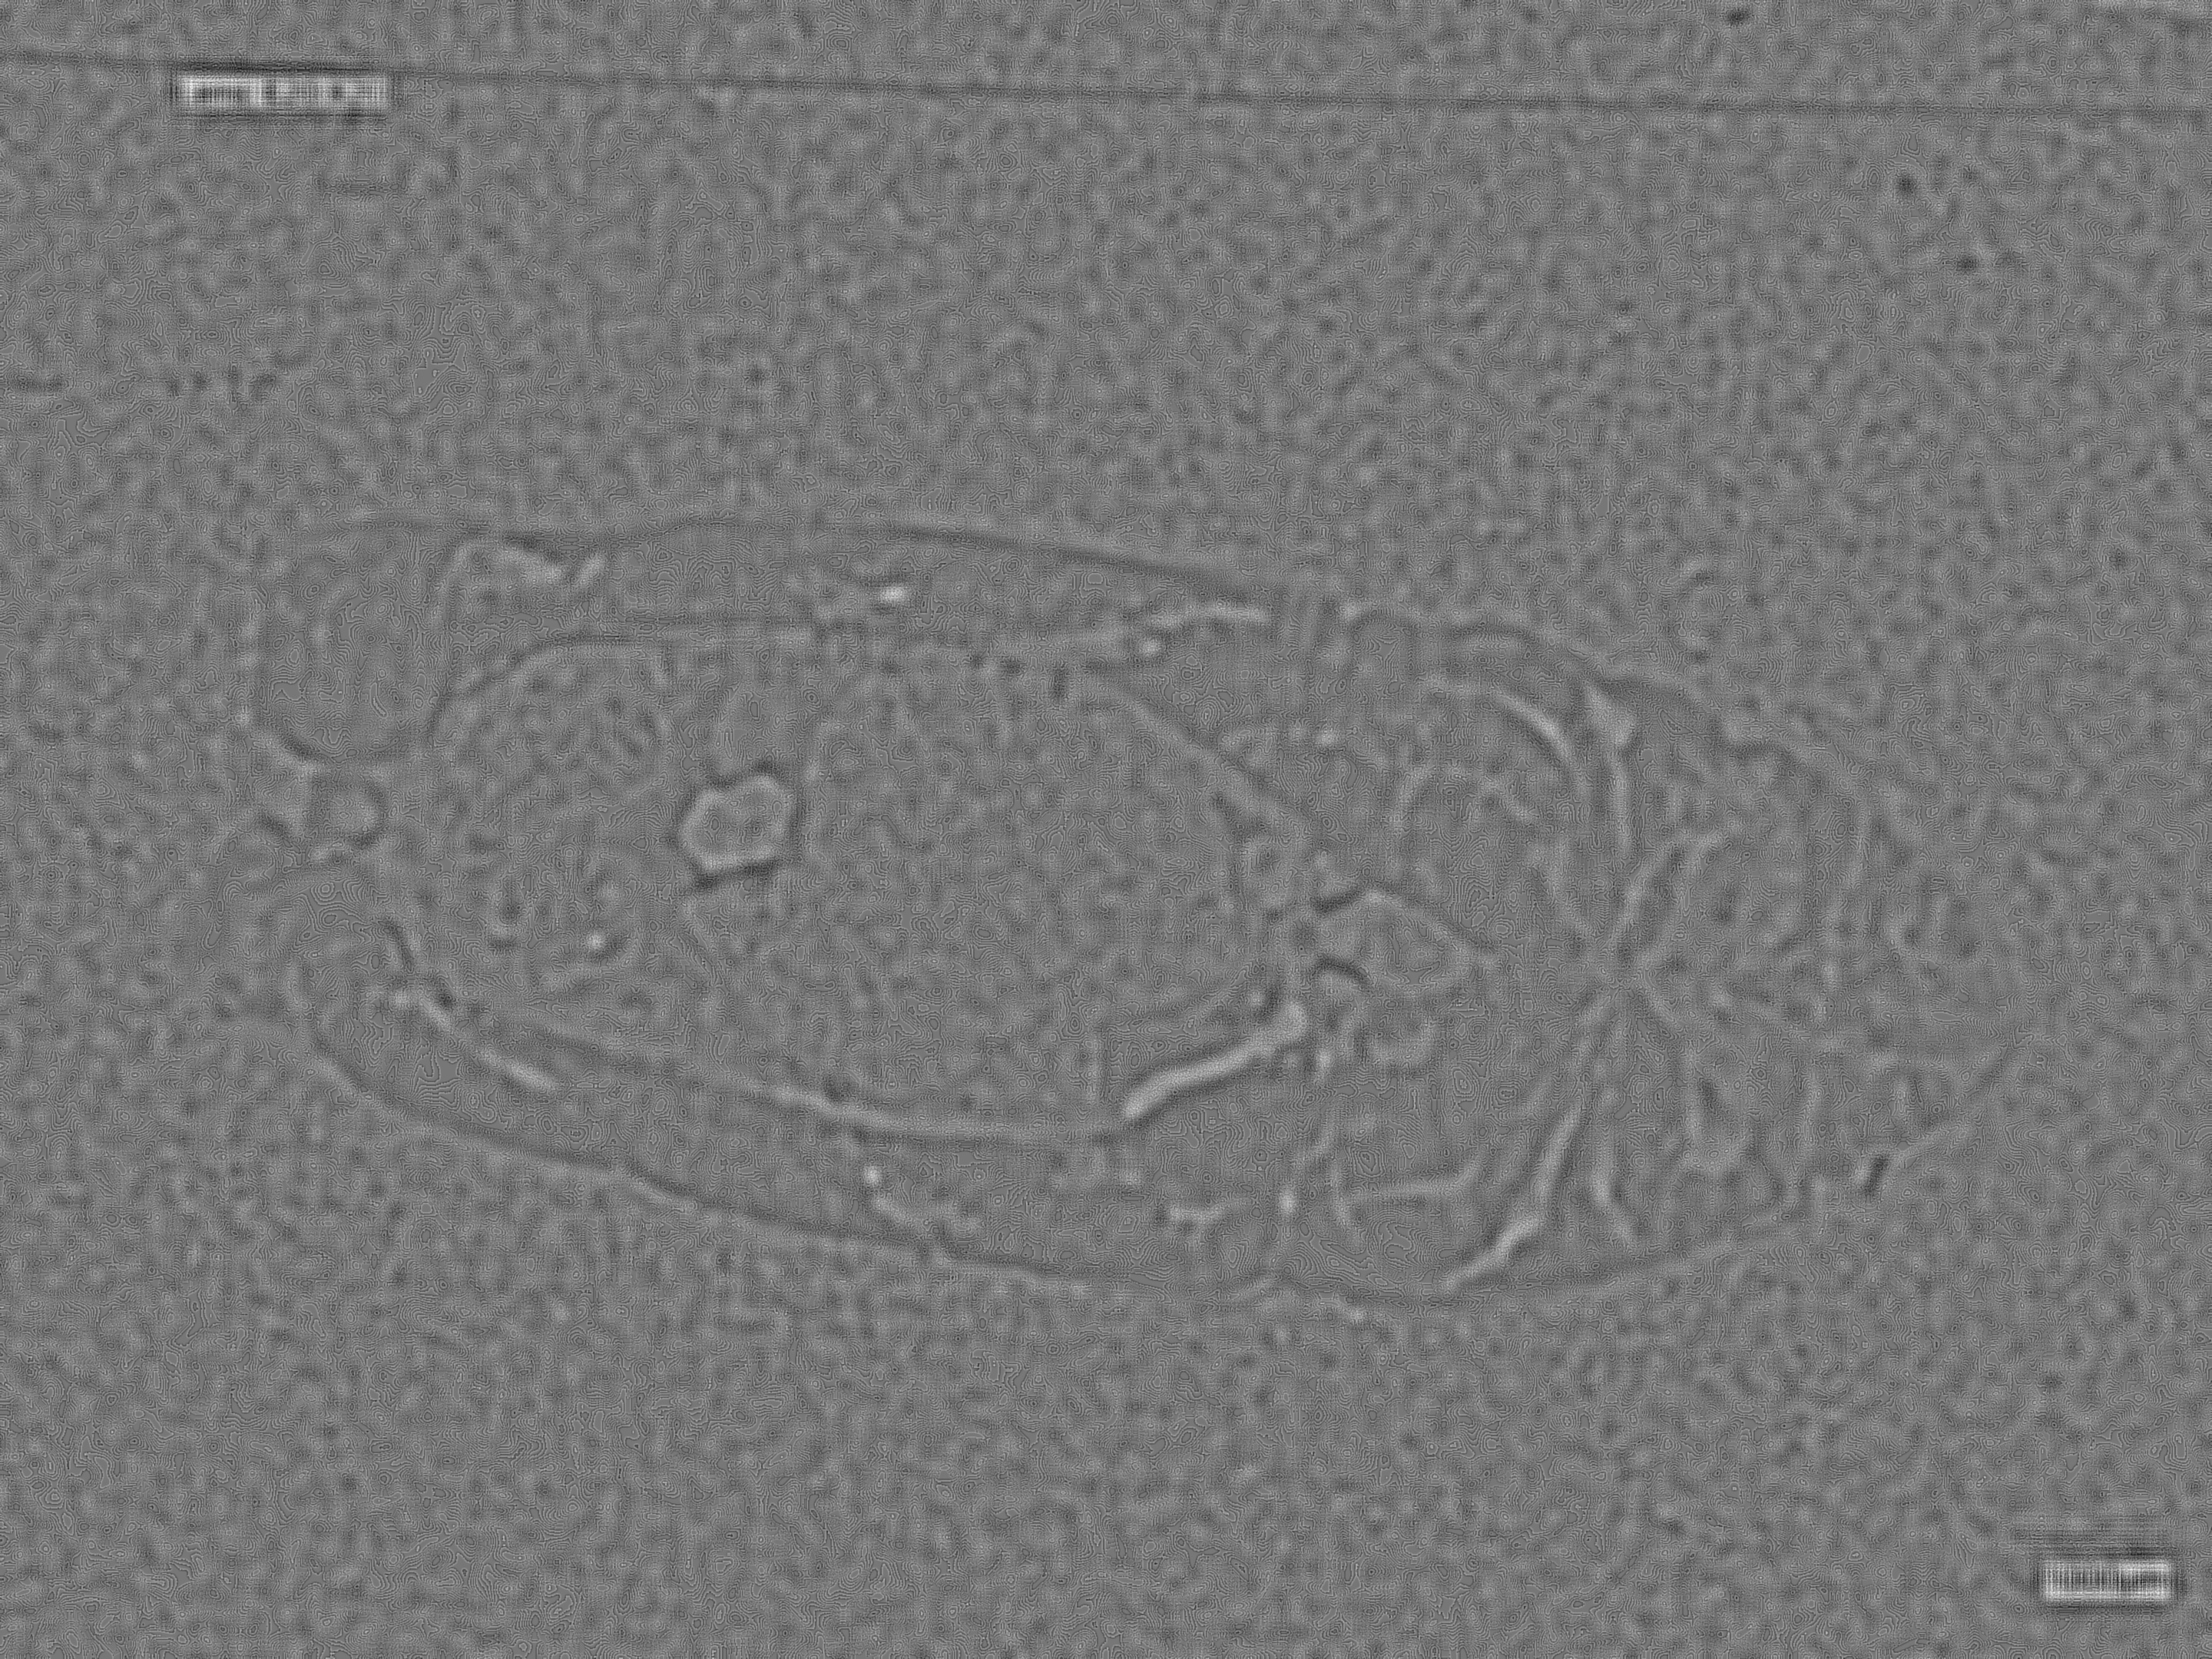
\includegraphics[width=\textwidth]{./fig/gausssian/laplacian61.jpg}
        \caption{laplacian}
        \label{fig:laplacian}
    \end{minipage}
\end{figure}

canny算法相对于sobel算法稍显复杂-引入了阈值检测,非极大值抑制等步骤。canny算法引入了两个阈值,分别为低阈值和高阈值。其中,当图像的梯度值大于高阈值时,被认为是边缘;当图像的梯度值小于低阈值时,被认为不是边缘;当图像的梯度值在两者之间时,如果与高阈值的边缘相连,则被认为是边缘,否则被认为不是边缘。这样的处理可以有效的去除图像中的噪声,得到更加准确的边缘检测结果。

%canny引用
通常情况下,高阈值和低阈值的比值在2:1到3:1之间。在这里我们选择阈值比为2.5 : 1,探究不同阈值对边缘检测的影响。

取低阈值为2 4 6 ,此时对应的高阈值为5 10 15 。canny算法的结果如下所示。

\begin{figure}
    \centering
    \begin{minipage}{0.45\textwidth}
        \centering
        \includegraphics[width=\textwidth]{./fig/gausssian/canny61+2.jpg}
        \caption{canny 2 5}
        \label{fig:canny2_5}
    \end{minipage}
    \begin{minipage}{0.45\textwidth}
        \centering
        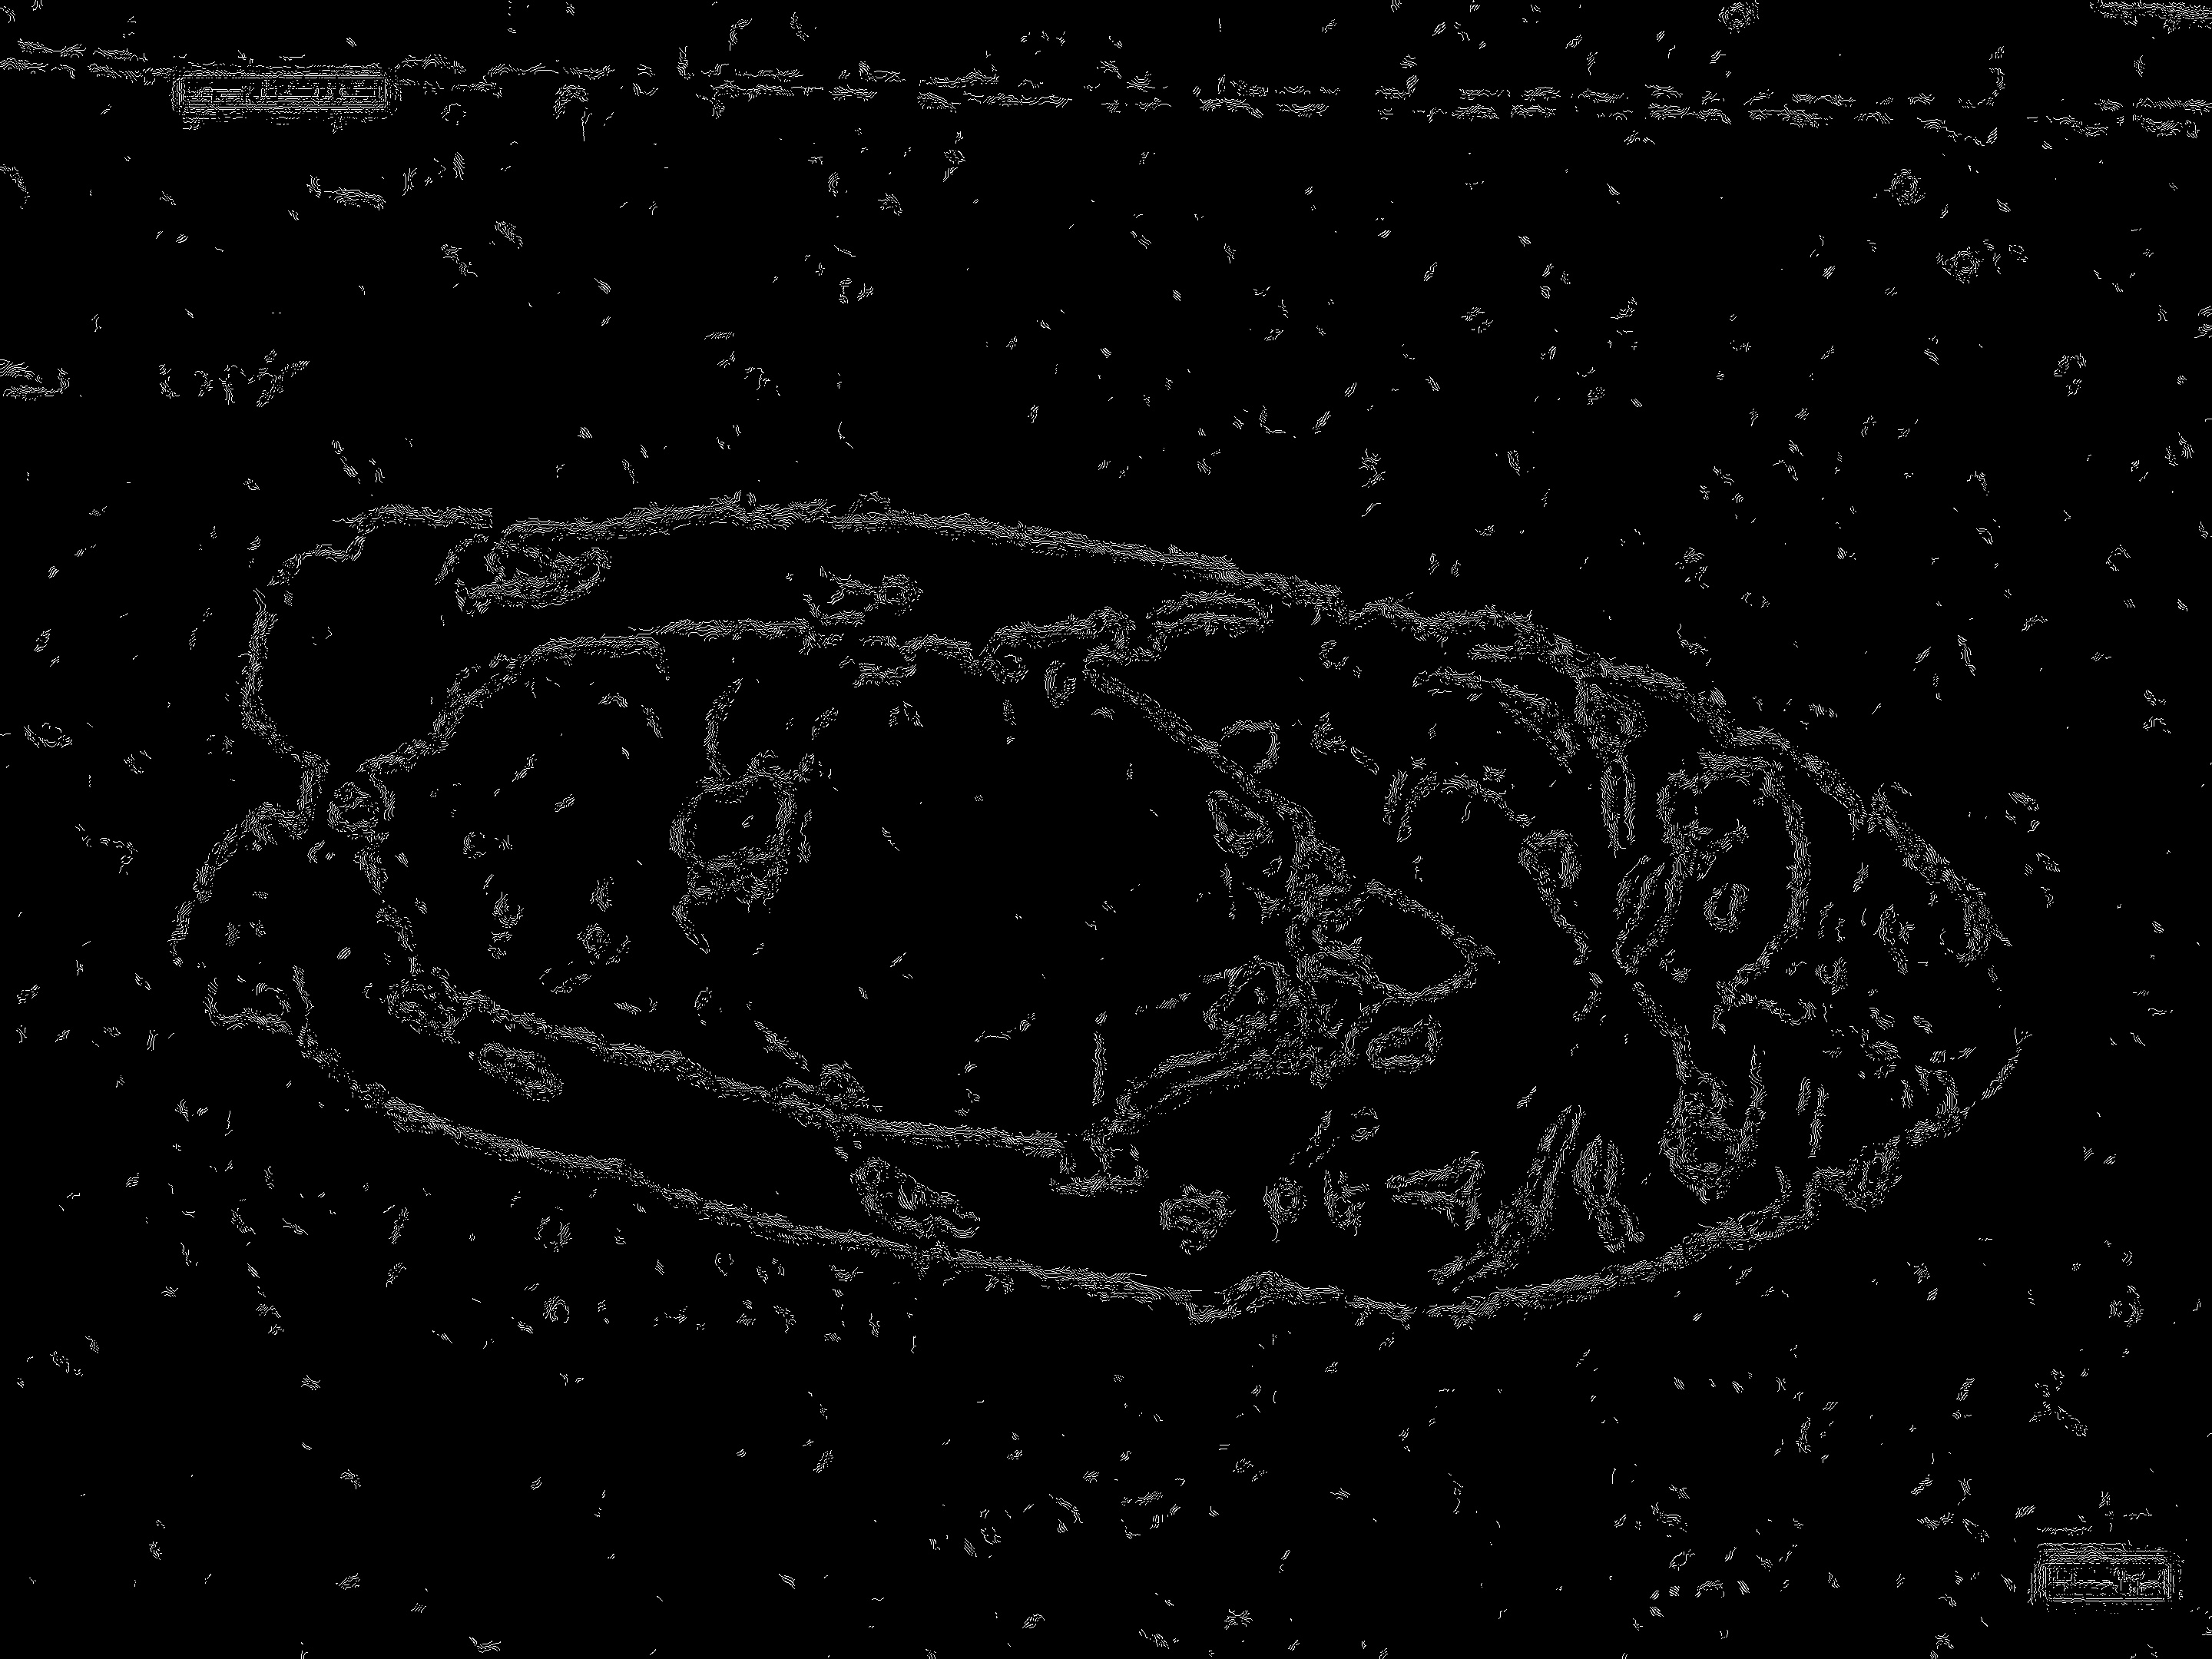
\includegraphics[width=\textwidth]{./fig/gausssian/canny61+4.jpg}
        \caption{canny 4 10}
        \label{fig:canny4_10}
    \end{minipage}
\end{figure}

\begin{figure}
    \centering
    \begin{minipage}{0.45\textwidth}
        \centering
        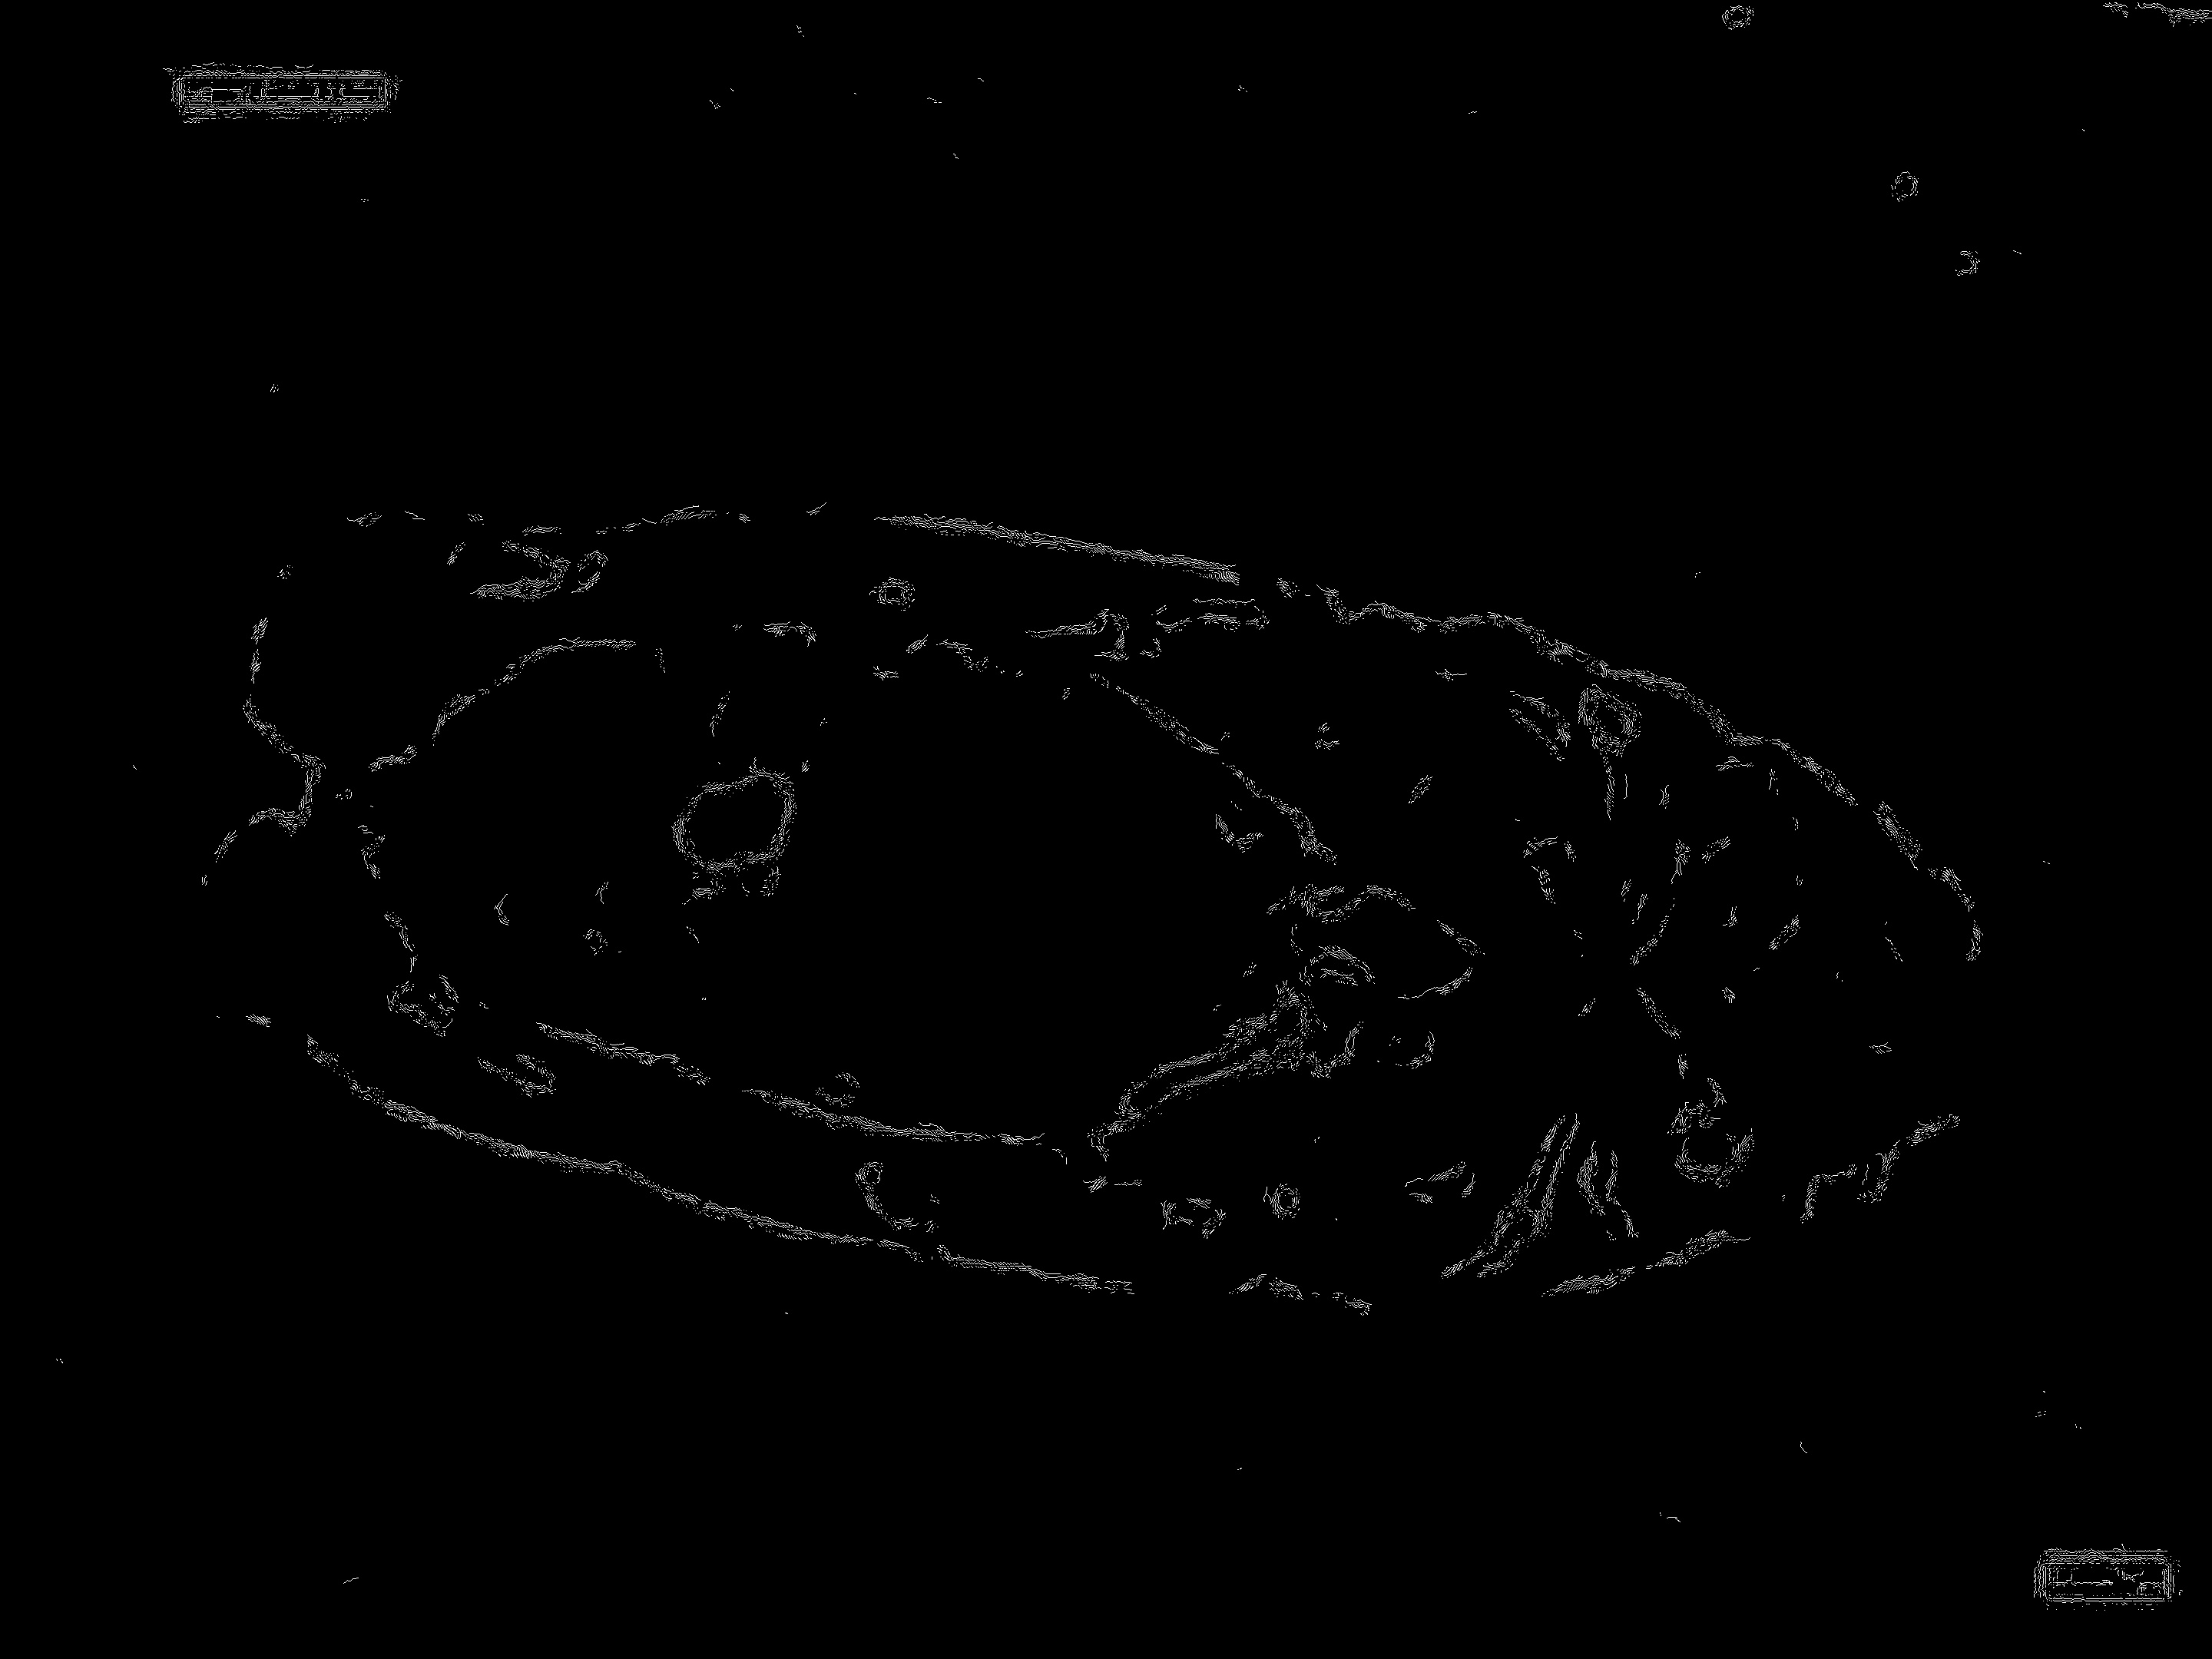
\includegraphics[width=\textwidth]{./fig/gausssian/canny61+6.jpg}
        \caption{canny 6 15}
        \label{fig:canny6_15}
    \end{minipage}
\end{figure}

在三张canny算法的结果中,可见\autoref{fig:canny4_10}的效果最好,其能在保证边缘细节得到大部分保留的情况下,去除了大部分的噪声。因此我们选择canny算法的阈值为4 10。

\textbf{总结}

对比sobel, laplacian和canny算法的结果,sobel算法的效果一般,对于底噪不是能很好的去除,边缘检测效果还算显著。laplacian算法最差,边缘甚至已经不可见,这可能是因为该算法对噪声最敏感。canny算法的效果最好,能够在保证边缘细节的情况下,去除大部分的噪声。因此我们选择canny算法作为图像预处理的方法。

\FloatBarrier


\subsubsection{阈值分割}

考虑到生物组织样本的主体是黄色,石蜡是白色,我们可以通过设置一个阈值,将图像中的白色部分分割出来,那么剩下的就是生物组织部分。在这里使用python的opencv库中进行操作。首先将图像进行对比度增强,增加饱和度,更好的凸显出生物组织的颜色(\autoref{fig:enhanced_image})。之后读取图像的每个像素点,将黄色周围半径15左右的像素点进行保留(约为图像宽的百分之一),其他的色块进行去除。(如\autoref{fig:yellowpic})。

\begin{figure}
    \centering
    \begin{minipage}{0.45\textwidth}
        \centering
        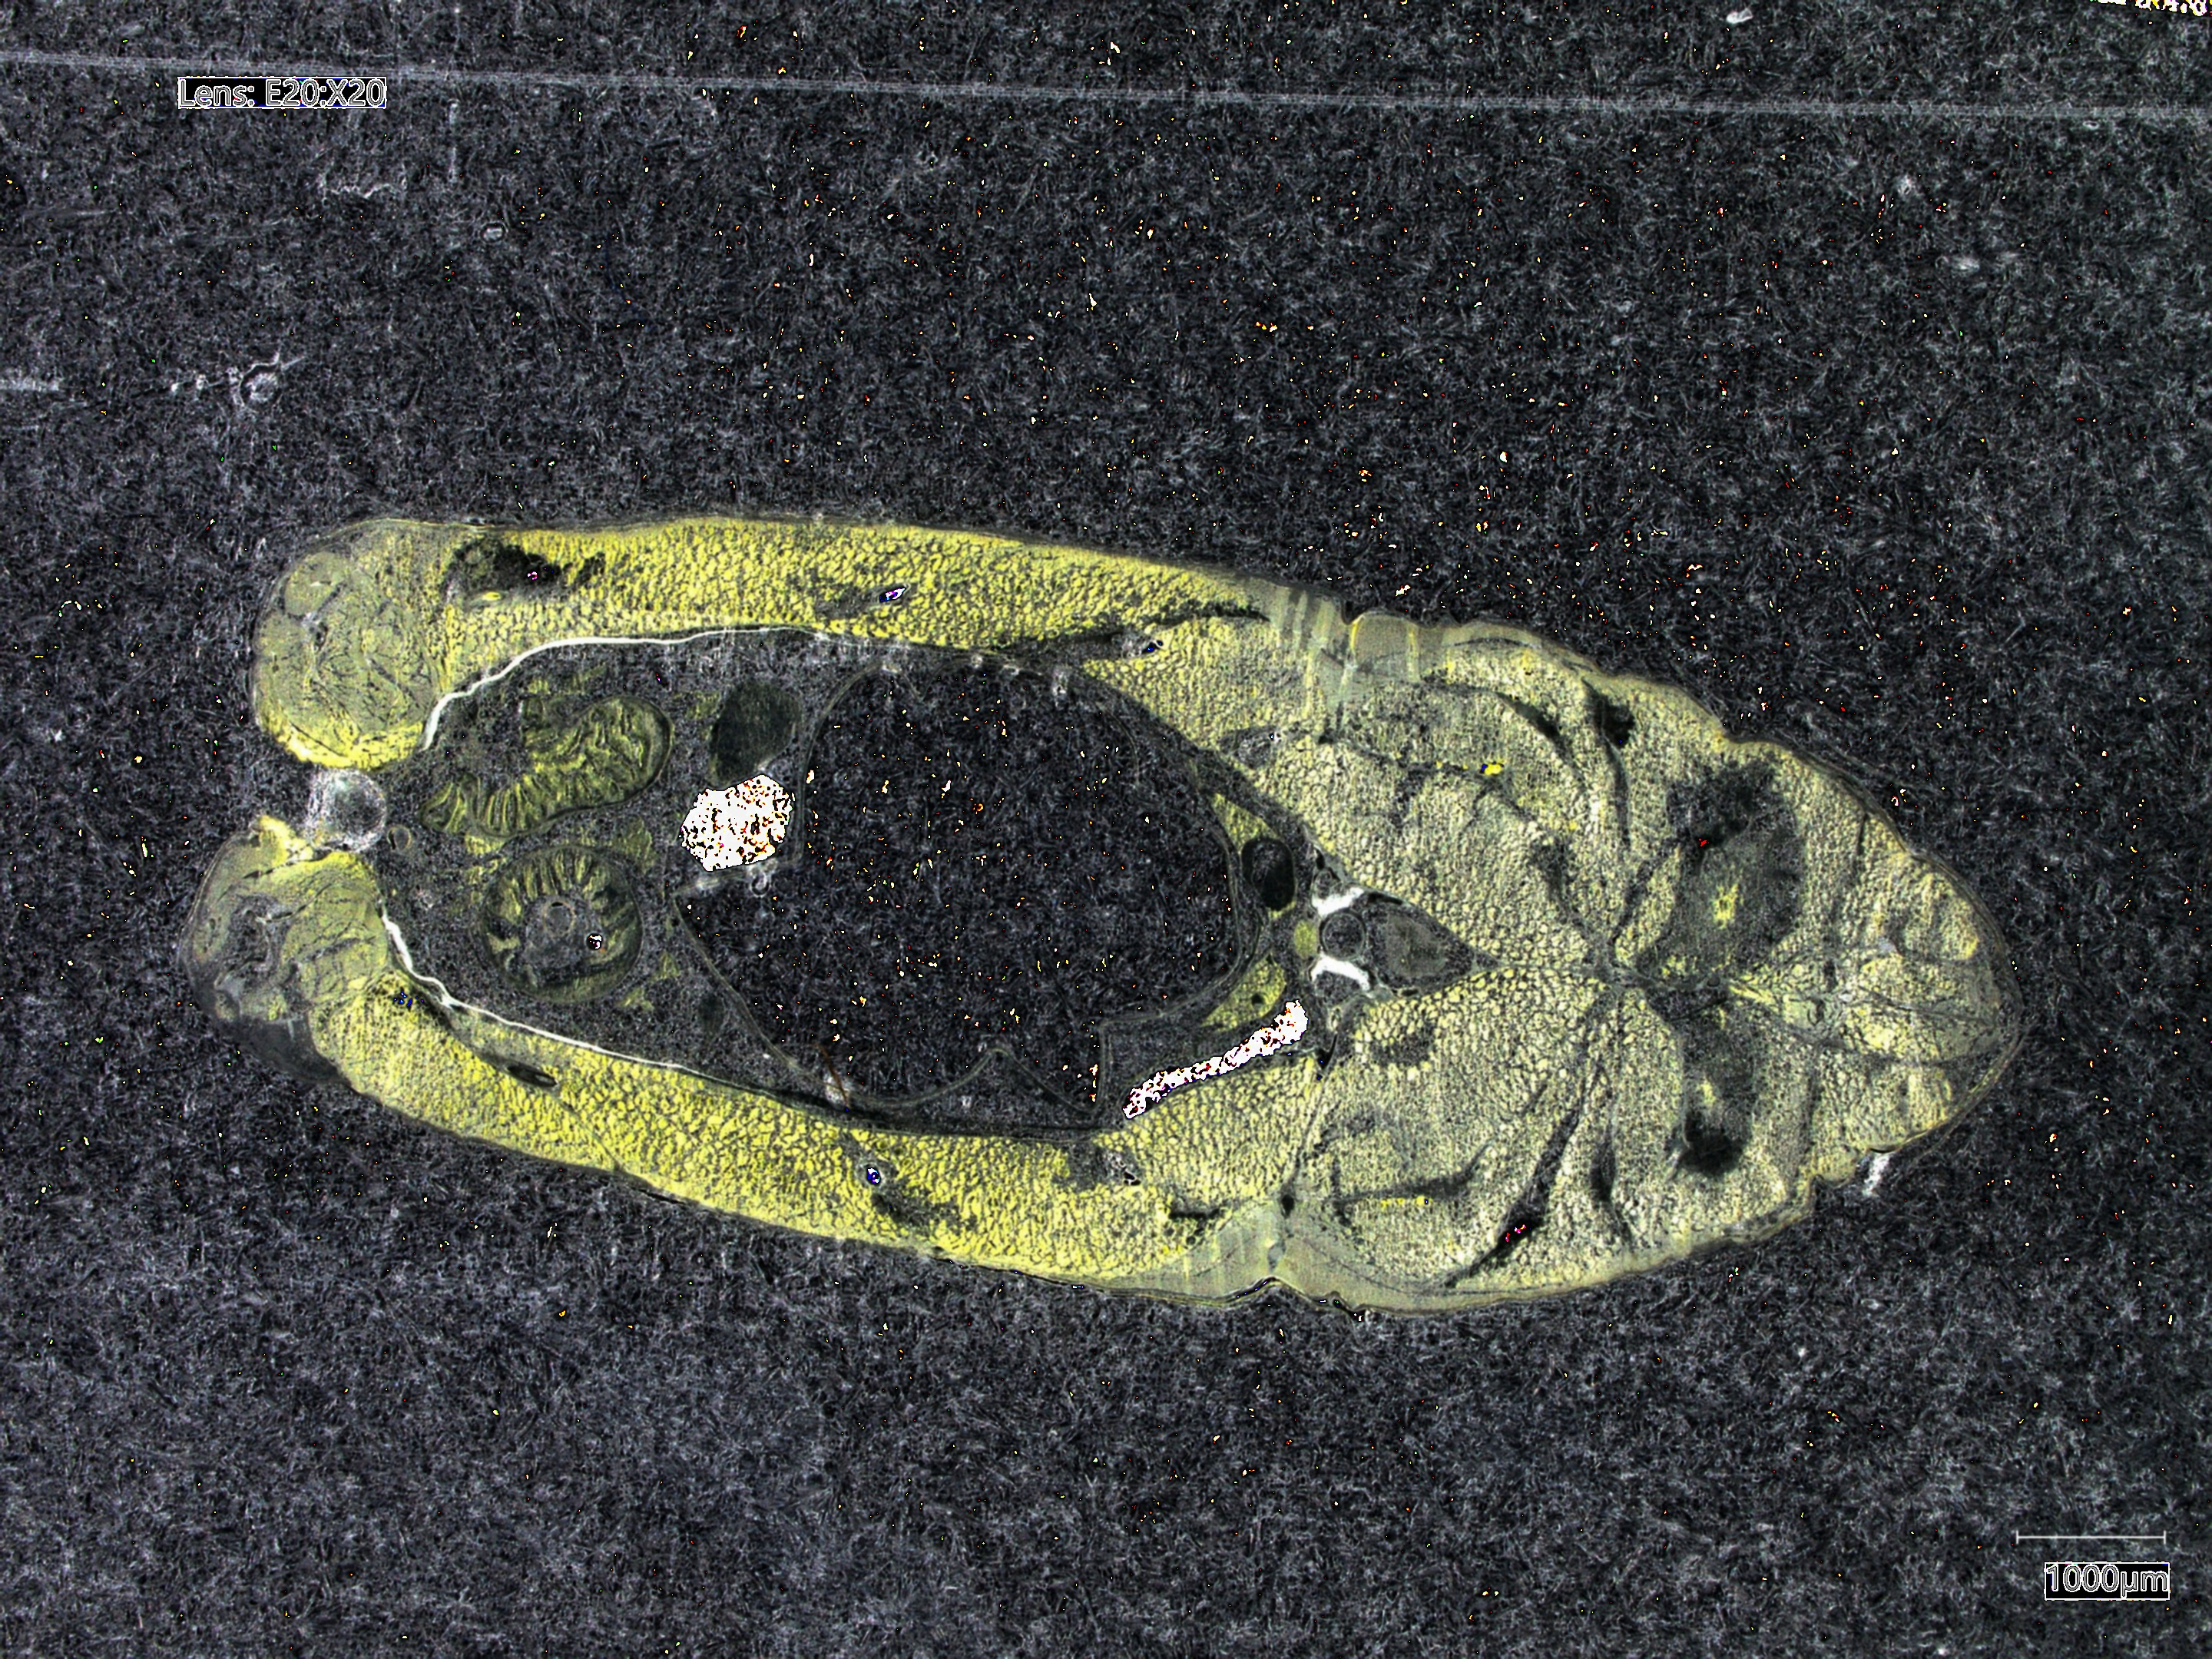
\includegraphics[width=\textwidth]{./fig/threshold/enhanced_image.jpg}
        \caption{enhanced image}
        \label{fig:enhanced_image}
    \end{minipage}
    \begin{minipage}{0.45\textwidth}
        \centering
        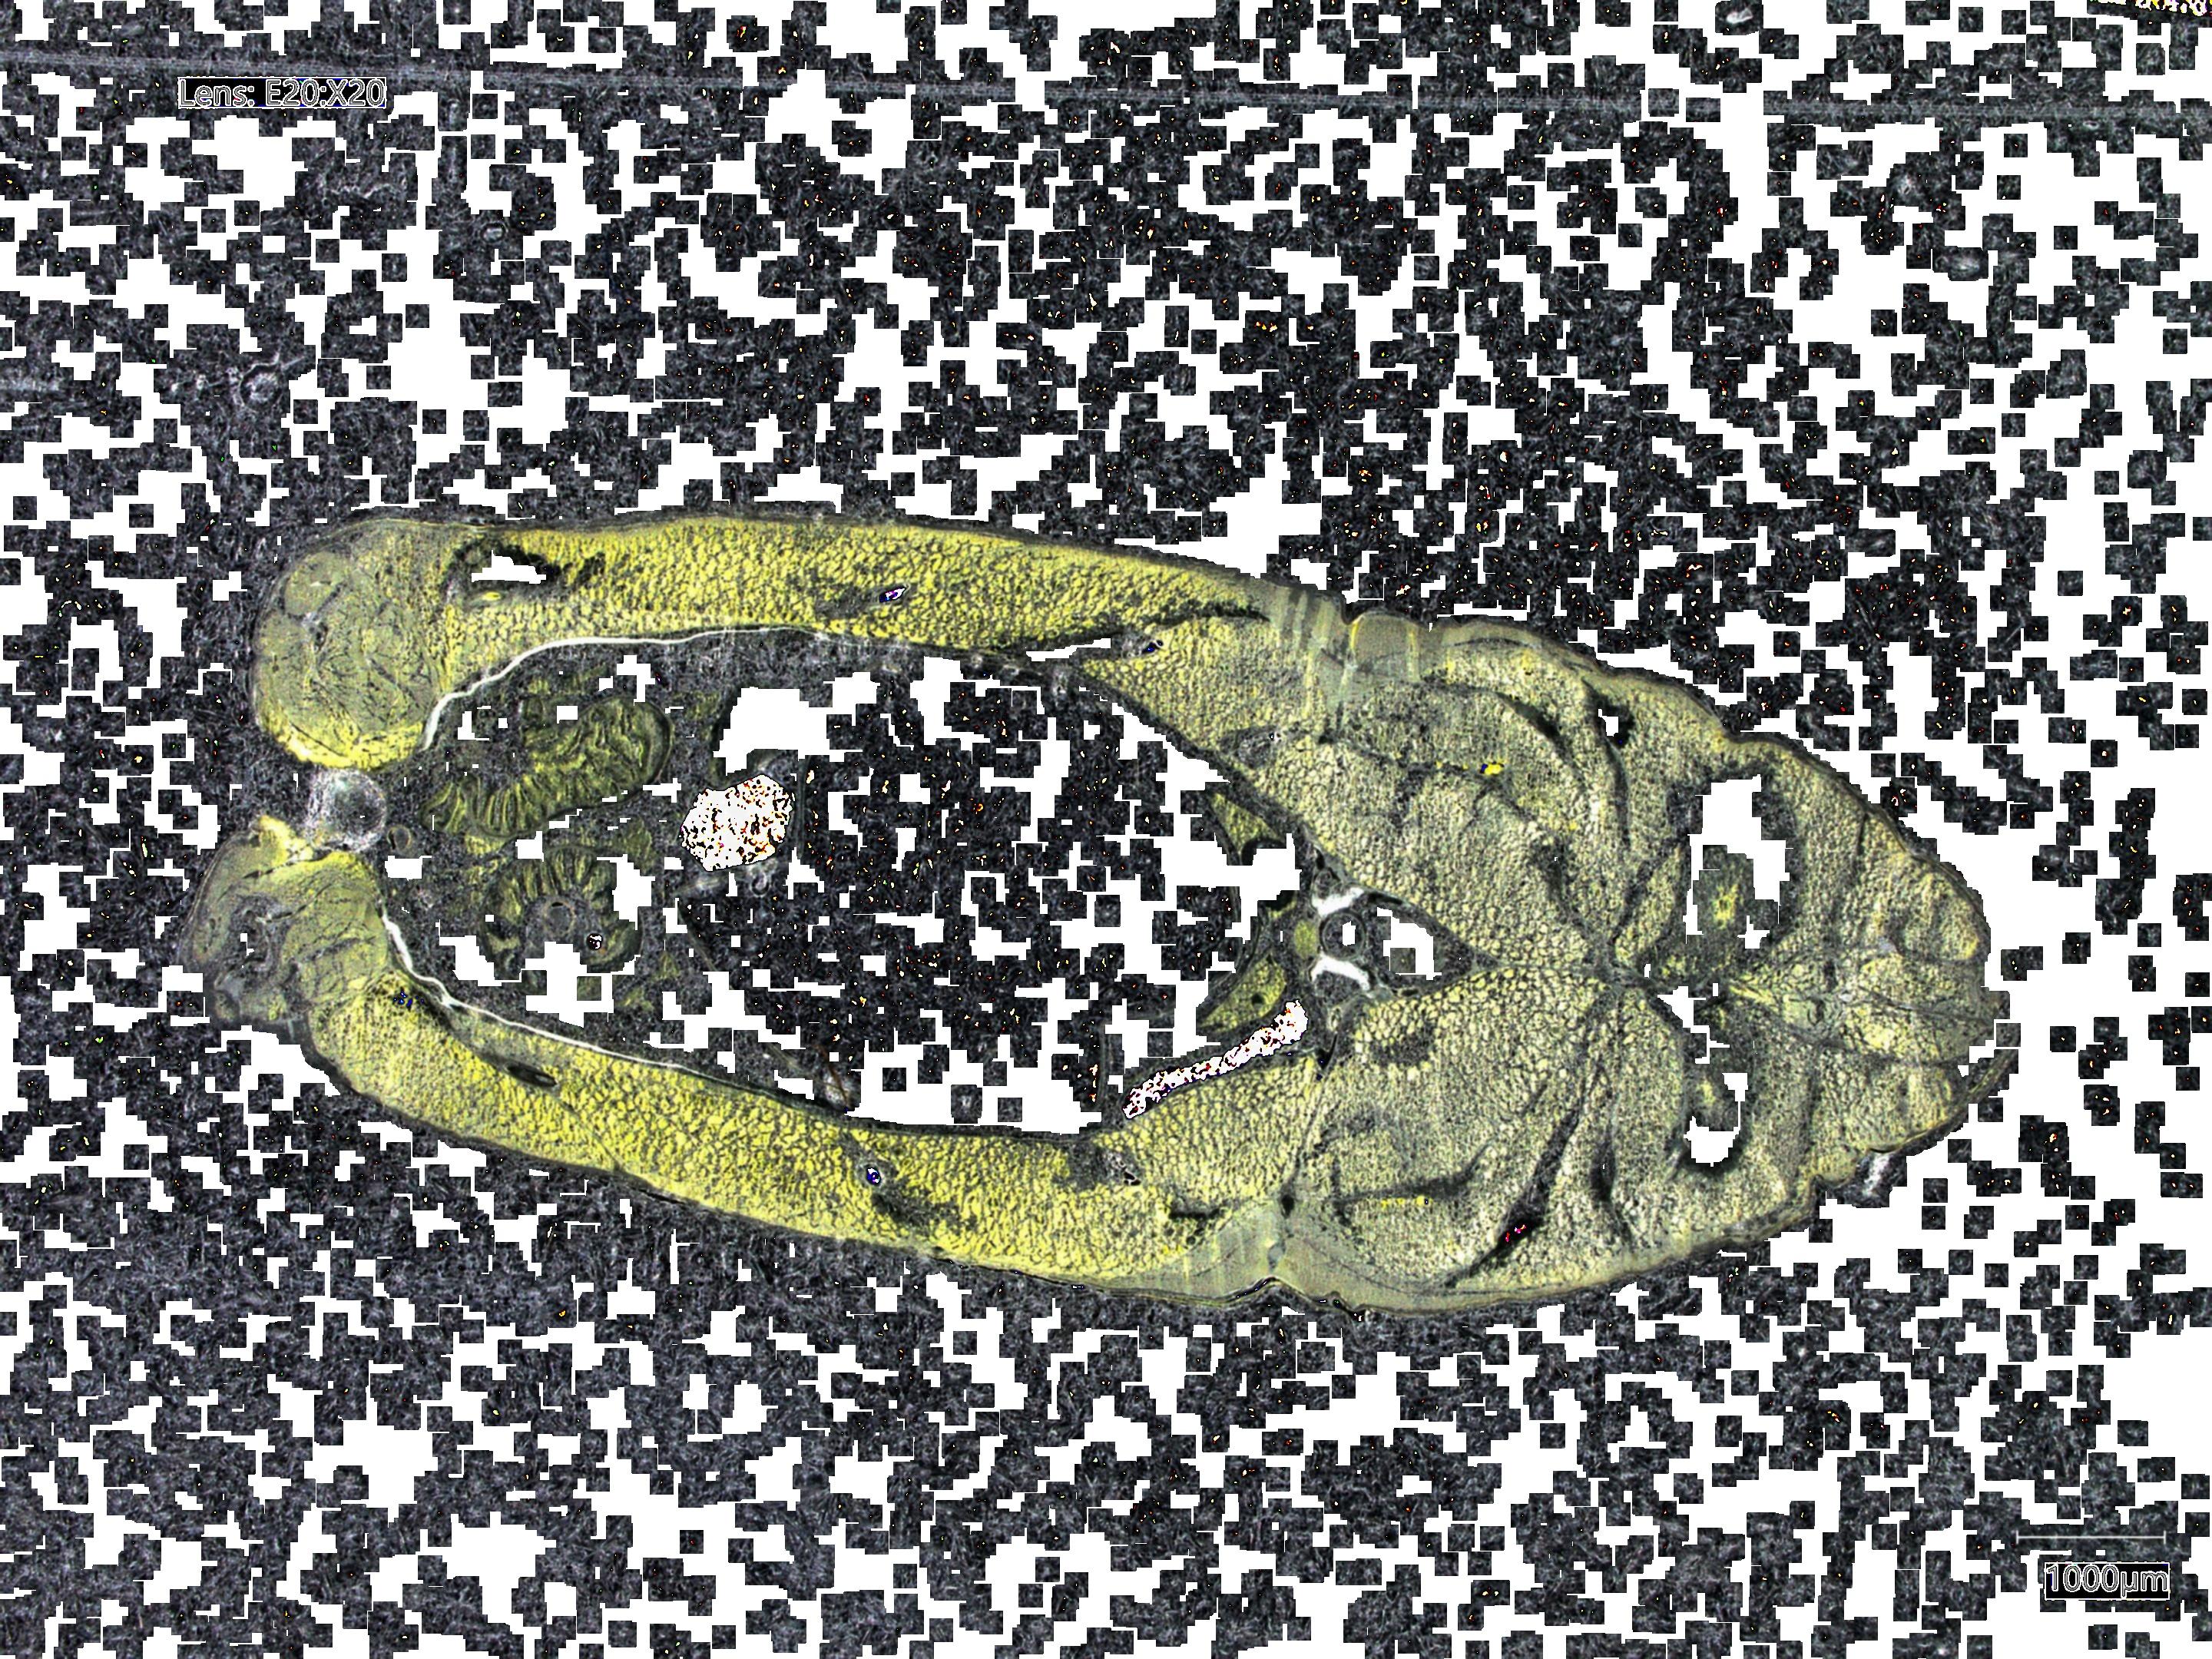
\includegraphics[width=\textwidth]{./fig/threshold/yellowpic.jpg}
        \caption{yellow picture}
        \label{fig:yellowpic}
    \end{minipage}
\end{figure}

但是观察发现,这种方法对于生物组织和石蜡的分割效果并不好,因为生物组织在切片过程中会掉落碎片组织,出现在标本各处,进而影响黄色像素点的识别。此时还需要进一步的处理,去除黑色色块。此时只需要将黑色色块进行掩码反转,使其变为白色即可。结果如图\autoref{fig:mask}所示。

\begin{figure}
    \centering
    \begin{minipage}{0.45\textwidth}
        \centering
        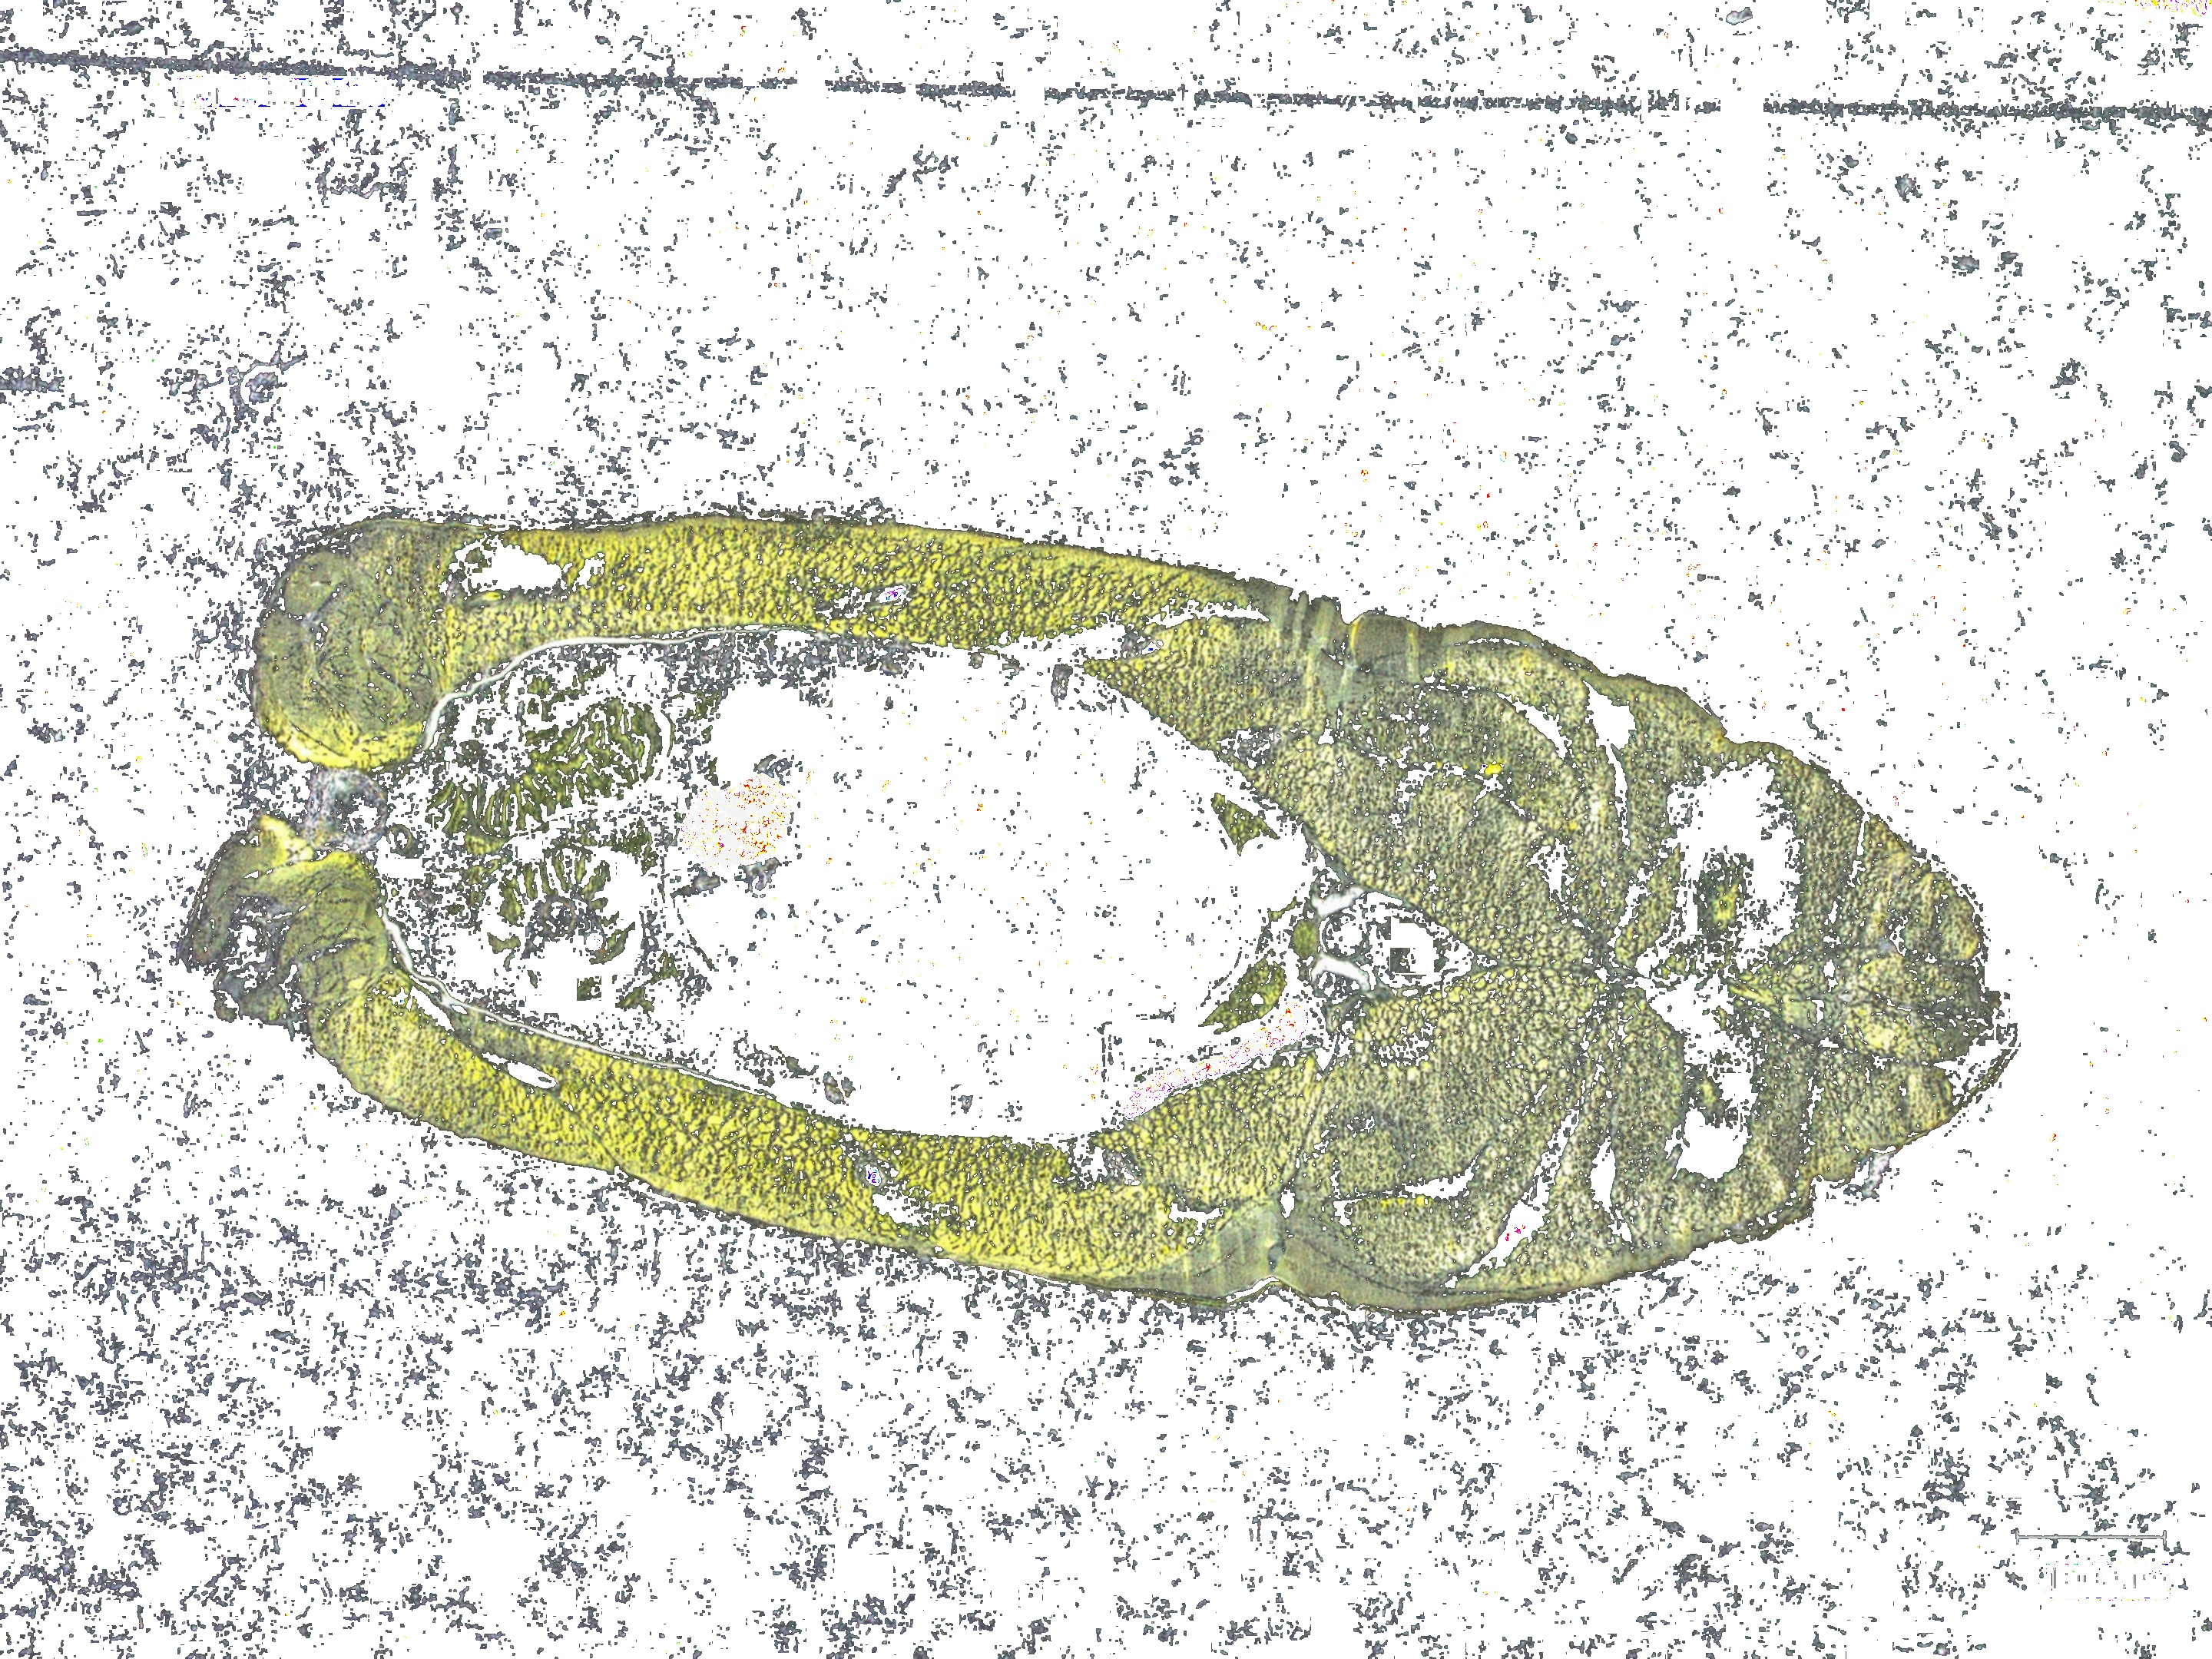
\includegraphics[width=\textwidth]{./fig/threshold/final.jpg}
        \caption{final}
        \label{fig:mask}
    \end{minipage}
    \begin{minipage}{0.45\textwidth}
        \centering
        \includegraphics[width=\textwidth]{./fig/threshold/fingerprint.jpg}
        \caption{fingerprint}
        \label{fig:fingerprint}
    \end{minipage}
\end{figure}

\subsubsection{另一种阈值分割方法-指纹算法}
在进行文献综述的时候,发现有一篇论文是基于otsu算法改进的分割方法用于进行指纹分割。考虑到切片样本和指纹都属于生物组织,因此我们尝试使用论文中提到的算法进行分割。结果如图\autoref{fig:fingerprint}所示。

\subsubsection{小结}
根据上文提到的图像预处理方法,我们可以看到,边缘检测和阈值分割的效果都不错,都能够很好的突出生物组织的特征,去除石蜡的干扰。对此我们可以设置三组数据集,分别是经过边缘检测后的图像,经过阈值分割后的图像和经过指纹算法分割后的图像。这三组数据集将作为我们的训练集,用于下一节的模型训练。

\FloatBarrier
\subsection{模型2:预处理图像+简单的cnn网络}

在这里基础模型选用在上一节模型1中表现相对比较好的模型1c。在这里我们将模型1c的输入改为经过预处理后的图像,即边缘检测后的图像,阈值分割后的图像和指纹算法分割后的图像。模型的架构不变,只是输入的数据发生了变化。

\subsubsection{model 2a}

模型2a采用和模型1c同样的架构构成,分别由三个包含32个特征图,卷积核为3*3的卷积层和最大池化层,一个包含256个神经元的全连接层组成。模型的输入为经过\textbf{canny边缘检测}后的图像。

模型训练的准确度和损失如\autoref{fig:model2a_acc}和\autoref{fig:model2a_loss}所示。

\begin{figure}
    \centering
    \begin{minipage}{0.45\textwidth}
        \centering
        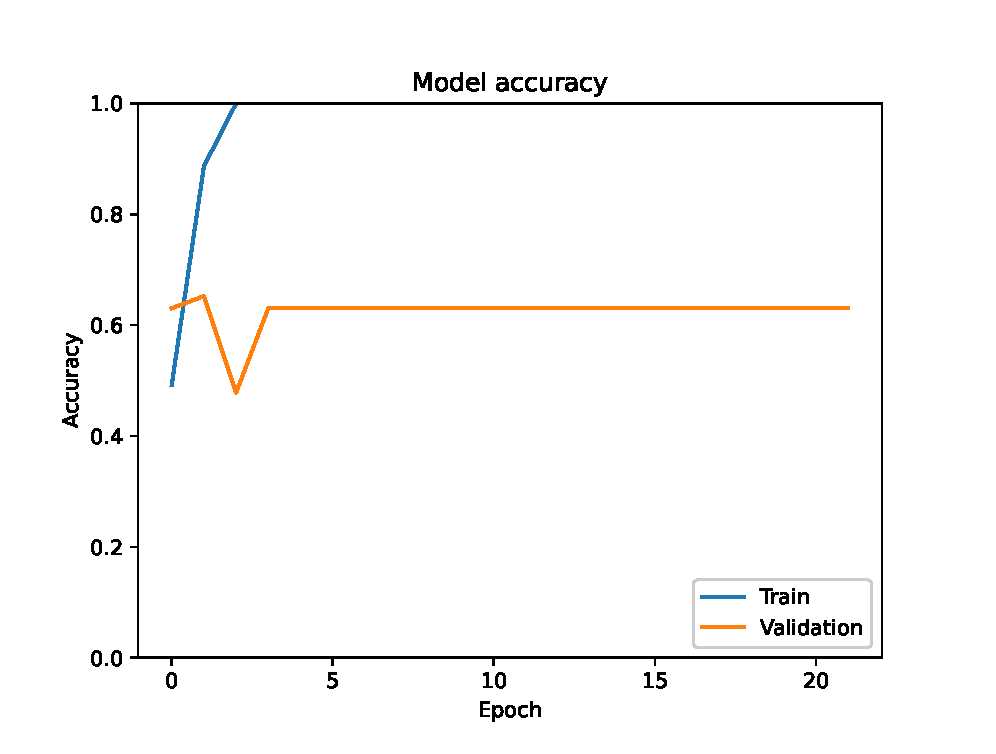
\includegraphics[width=\textwidth]{./fig/model2/accuracy2a.eps}
        \caption{Model-2a accuracy}
        \label{fig:model2a_acc}
    \end{minipage}
    \begin{minipage}{0.45\textwidth}
        \centering
        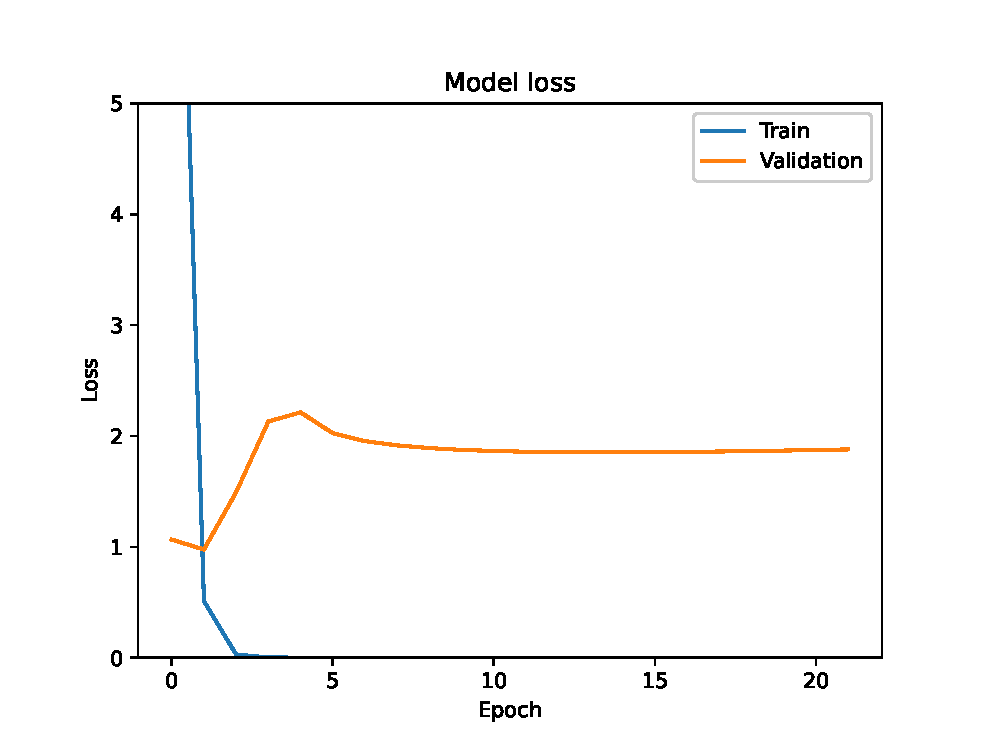
\includegraphics[width=\textwidth]{./fig/model2/loss2a.eps}
        \caption{Model-2a loss}
        \label{fig:model2a_loss}
    \end{minipage}
\end{figure}



\subsubsection{model 2b}

模型2b采用和模型1c同样的架构构成但是模型的输入为经过\textbf{阈值分割}后的图像。

模型训练的准确度和损失如\autoref{fig:model2b_acc}和\autoref{fig:model2b_loss}所示。

\begin{figure}
    \centering
    \begin{minipage}{0.45\textwidth}
        \centering
        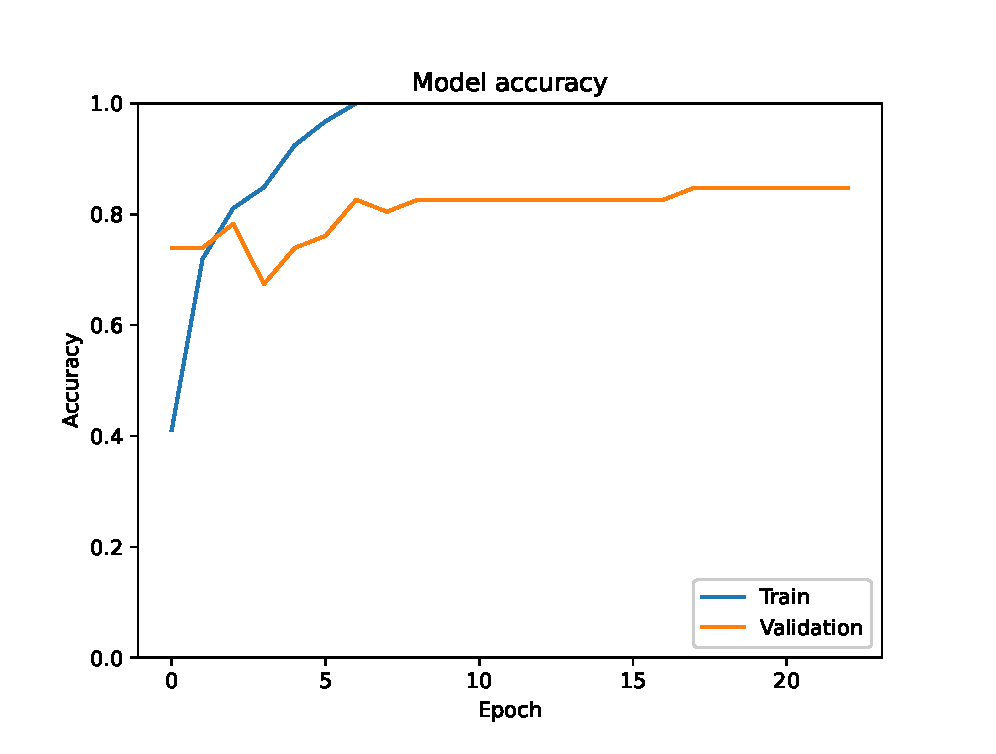
\includegraphics[width=\textwidth]{./fig/model2/accuracy2b.eps}
        \caption{Model-2b accuracy}
        \label{fig:model2b_acc}
    \end{minipage}
    \begin{minipage}{0.45\textwidth}
        \centering
        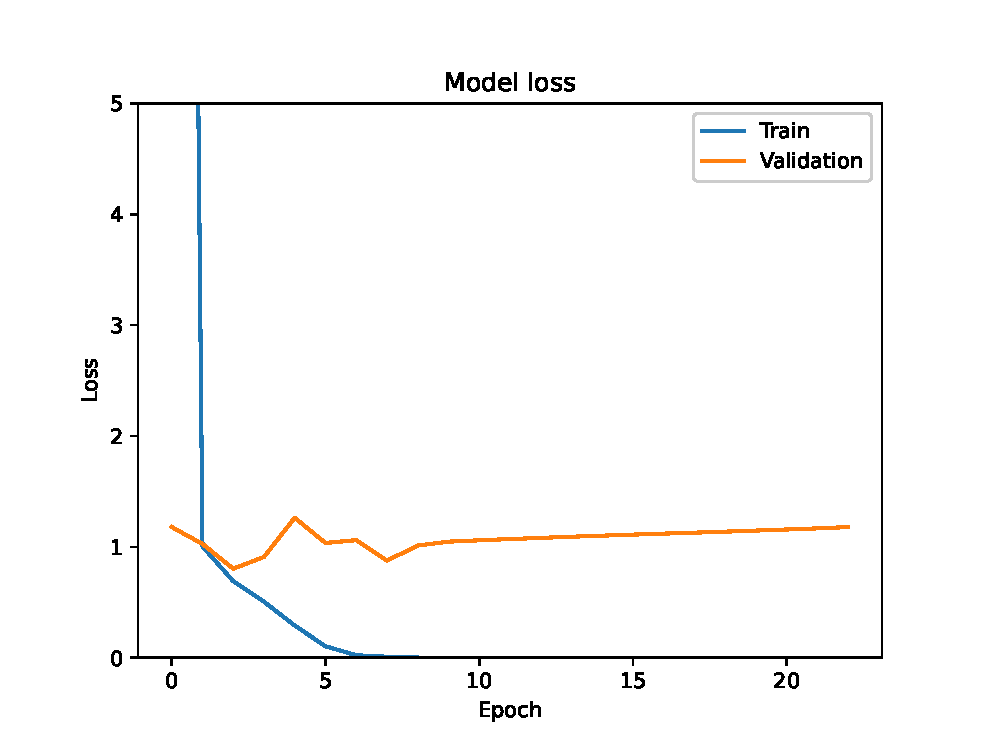
\includegraphics[width=\textwidth]{./fig/model2/loss2b.eps}
        \caption{Model-2b loss}
        \label{fig:model2b_loss}
    \end{minipage}
\end{figure}


\subsubsection{model 2c}

模型2c采用和模型1c同样的架构构成但是模型的输入为经过\textbf{指纹算法分割}后的图像。

模型训练的准确度和损失如\autoref{fig:model2c_acc}和\autoref{fig:model2c_loss}所示。

\begin{figure}
    \centering
    \begin{minipage}{0.45\textwidth}
        \centering
        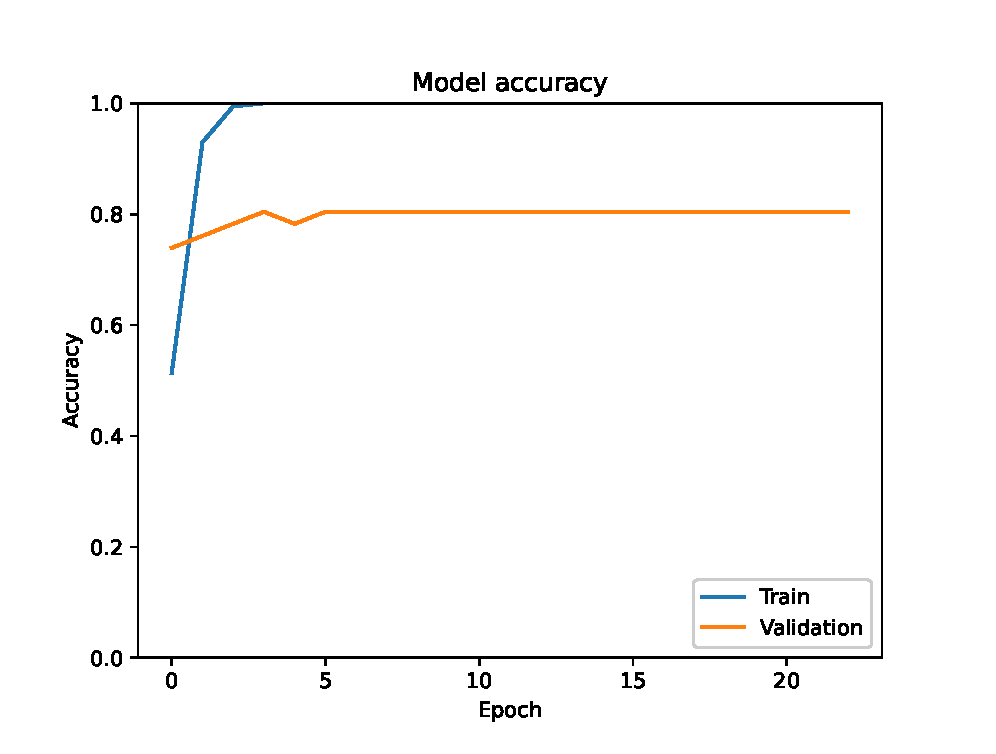
\includegraphics[width=\textwidth]{./fig/model2/accuracy2c.eps}
        \caption{Model-2c accuracy}
        \label{fig:model2c_acc}
    \end{minipage}
    \begin{minipage}{0.45\textwidth}
        \centering
        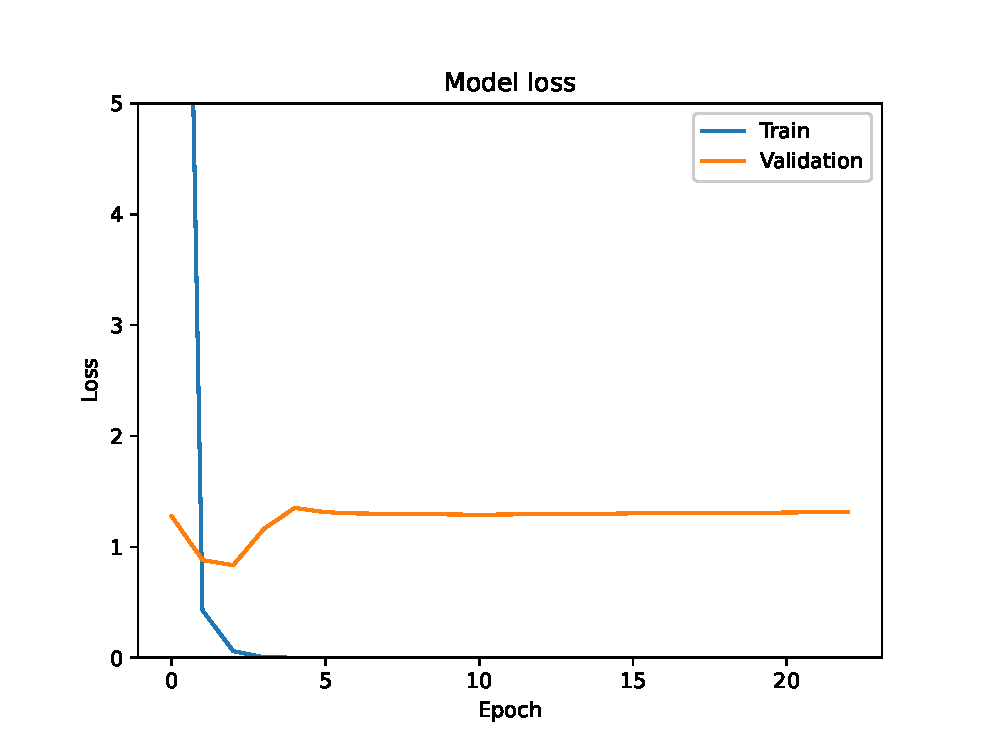
\includegraphics[width=\textwidth]{./fig/model2/loss2c.eps}
        \caption{Model-2c loss}
        \label{fig:model2c_loss}
    \end{minipage}
\end{figure}



\subsubsection{小结}
对比模型2a 2b 2c,可以发现模型2a和模型2c在训练步长为5之后就开始收敛,其训练准确度和验证准确度收敛于1和0.8左右。但是损失确仍然较高,这说明模型在训练集上表现良好,但是在验证集上表现欠佳。

模型2b在训练步长为10之后也开始收敛,但是其训练准确度和验证准确度收敛于1和0.8左右,损失收敛于1左右。这说明模型2b表现显著优于模型2a和模型2c。

这可能的原因是模型2a和2c的输入是灰度图,即图像复杂度显著小于彩色图,而模型2b的输入是彩色图,因此在模型提取特征时还能够参考根据色块的rgb值进行提取,故模型2b的表现最好。

但是,在训练过程中,我们发现对于部分图像,经过模型2(特别是2b)的前处理(阈值分割)后,图像的部分重要细节会丢失,进而影响图像标签的准确性。例子如下所示:

\begin{figure}
    \centering
    \begin{minipage}{0.45\textwidth}
        \centering
        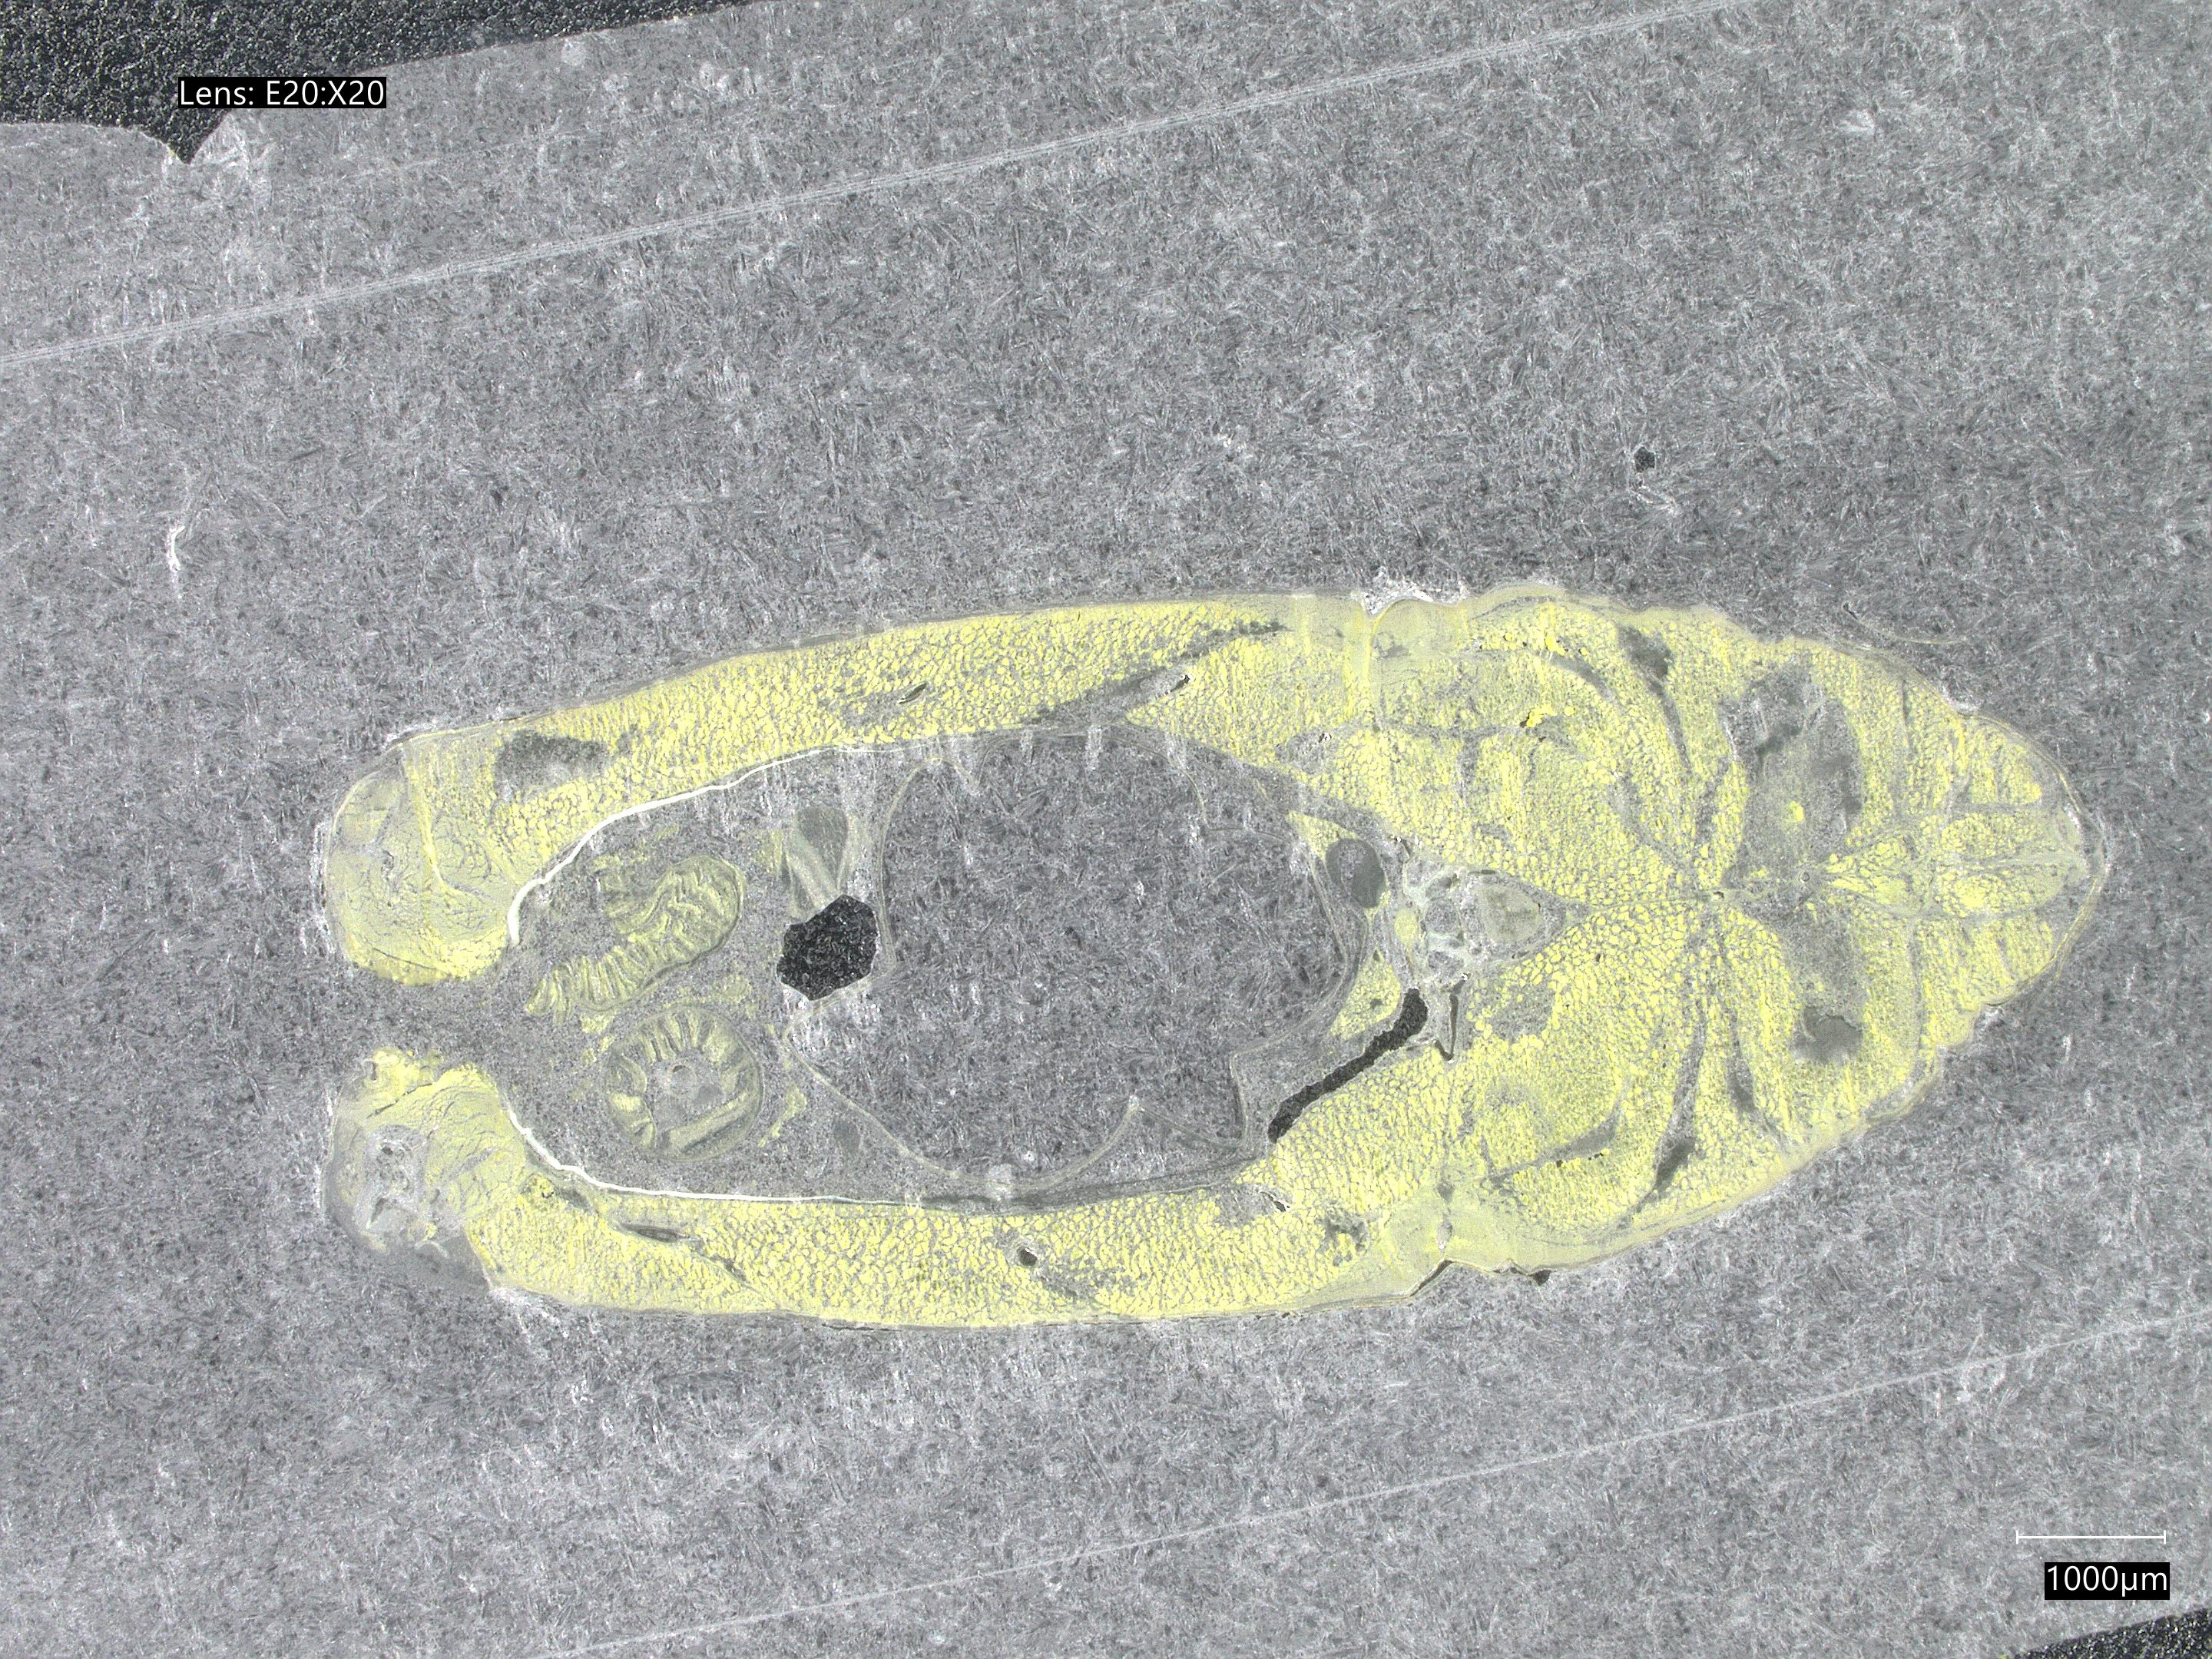
\includegraphics[width=\textwidth]{./fig/model2/origin20240205_161427.jpg}
        \caption{origin}
        \label{fig:origin}
    \end{minipage}
    \begin{minipage}{0.45\textwidth}
        \centering
        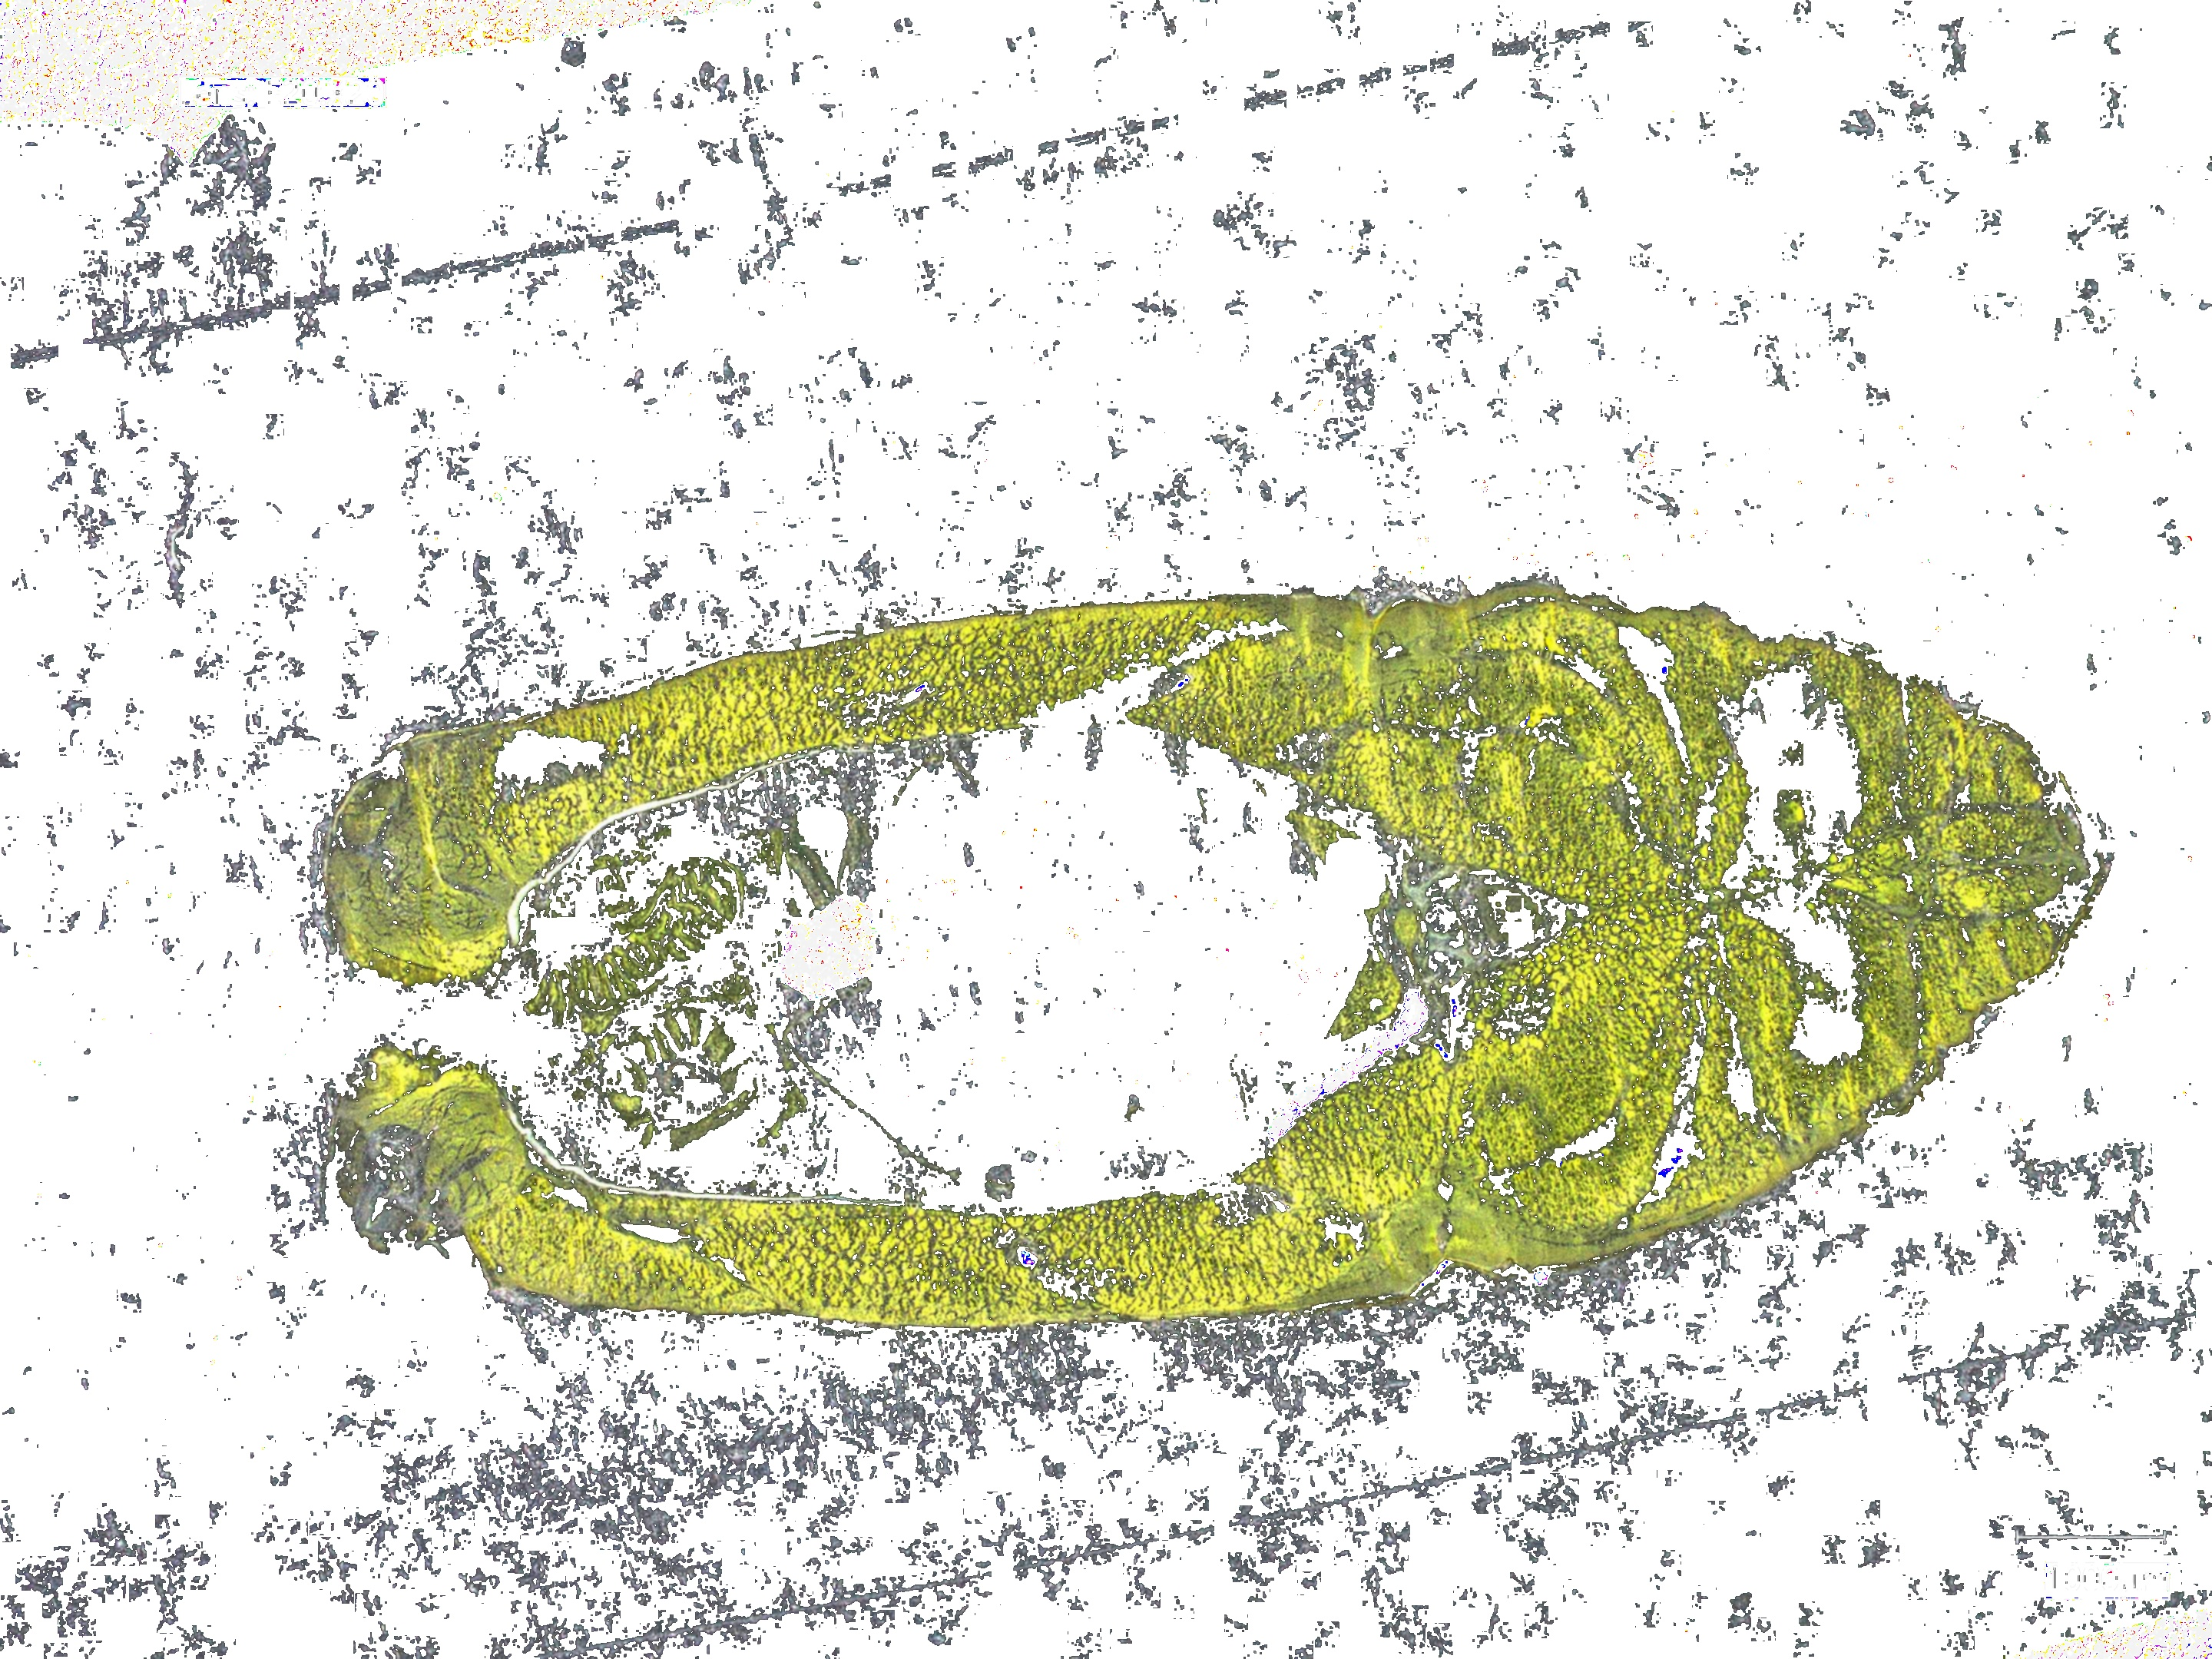
\includegraphics[width=\textwidth]{./fig/model2/yellow20240205_161427.jpg}
        \caption{yellow}
        \label{fig:yellow}
    \end{minipage}
\end{figure}

\autoref{fig:yellow}是模型2b训练集(经过黄色阈值分割后的图像)中的一张图片,对比原图(\autoref{fig:origin})可以观察发现,原本切片中能够被接受的平行白线被阈值分割算法显著增强了,这有极有可能会影响模型的训练效果,即模型会在一定程度上与horizental line混淆。

此外,经过图像前处理过的图像,还会在一定程度上丢失部分细节,这也会影响模型的训练效果。因此,图像前处理的方法虽然能够在一定程度上提高模型的训练效果,但是也会在一定程度上影响模型的训练效果。因此,我们需要进一步的改进模型,以提高模型的训练效果。

\FloatBarrier
\subsection{模型3:原始图像+迁移学习}

现在我们已经尝试过了简单的cnn网络,以及对图像进行预处理后的cnn网络。既然训练结果不是很理想,那我们为什么不去尝试更大更深的模型? 在这一节,我们尝试使用迁移学习的方法,使用预训练好的大规模深度学习模型,将其迁移到我们的数据集上,以提高模型的训练效果。

正如在第三节methodology里提到的,在这里将使用VGG16,VGG19和InceptionV3三个模型进行迁移学习。这三个模型都是在ImageNet数据集上训练好的模型,具有已经训练好的权重。

在这里为了避免过拟合,不仅使用了原有的早停法,还限制了模型的学习率(1e-5)

model3a是使用VGG16模型进行迁移学习的模型,model3b是使用VGG19模型进行迁移学习的模型,model3c是使用InceptionV3模型进行迁移学习的模型。

\subsubsection{model 3a}
根据VGG16的训练架构,输入层应该为224*224的图像,因此我们需要将图像的分辨率调整为224*224。

模型训练的准确度和损失如\autoref{fig:model3a_acc}和\autoref{fig:model3a_loss}所示

\begin{figure}
    \centering
    \begin{minipage}{0.45\textwidth}
        \centering
        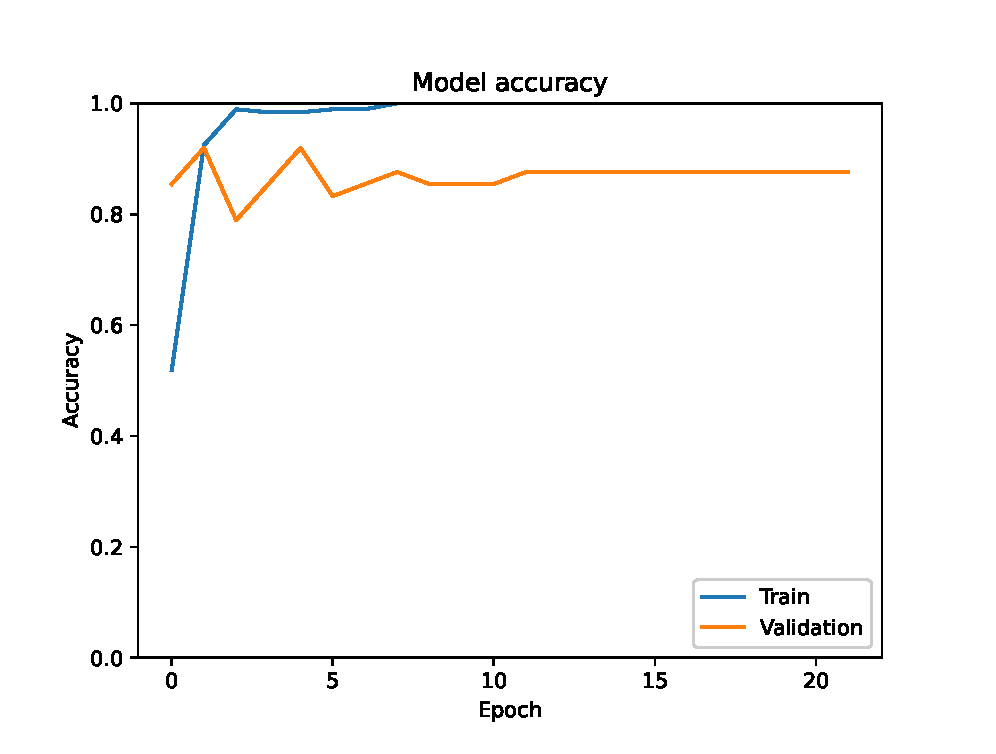
\includegraphics[width=\textwidth]{./fig/model3/accuracy3a.eps}
        \caption{Model-3a accuracy}
        \label{fig:model3a_acc}
    \end{minipage}
    \begin{minipage}{0.45\textwidth}
        \centering
        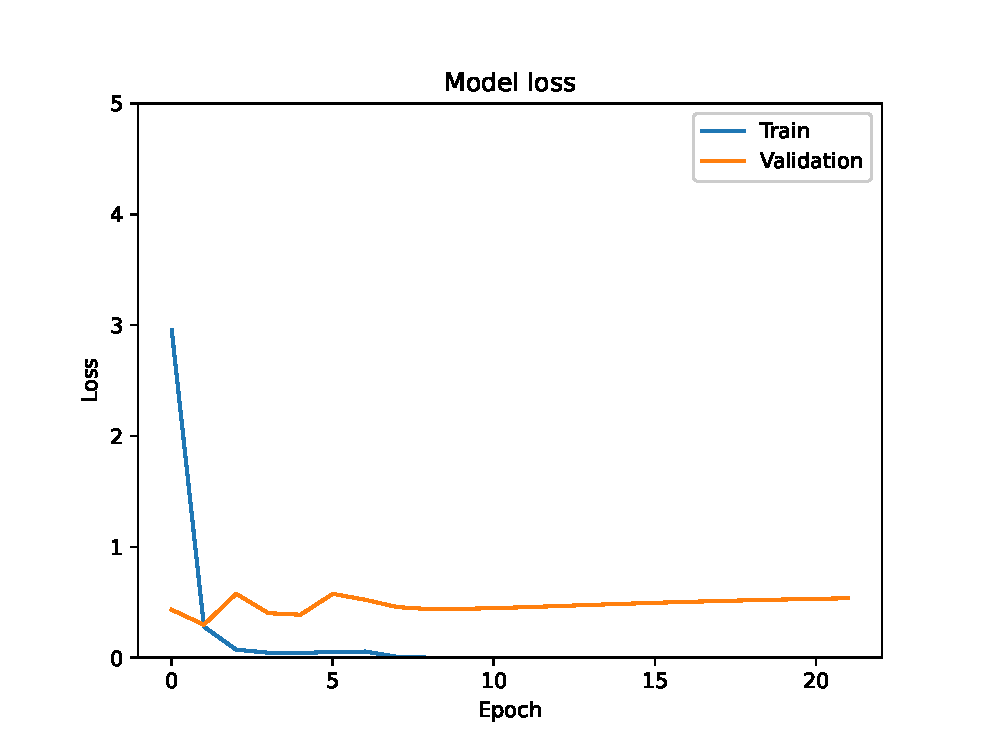
\includegraphics[width=\textwidth]{./fig/model3/loss3a.eps}
        \caption{Model-3a loss}
        \label{fig:model3a_loss}
    \end{minipage}
\end{figure}

\subsubsection{model 3b}
VGG19和VGG16相比只是在中间增加了3个额外的卷积层,其他与VGG16相同。模型训练的准确度和损失如\autoref{fig:model3b_acc}和\autoref{fig:model3b_loss}所示

\begin{figure}
    \centering
    \begin{minipage}{0.45\textwidth}
        \centering
        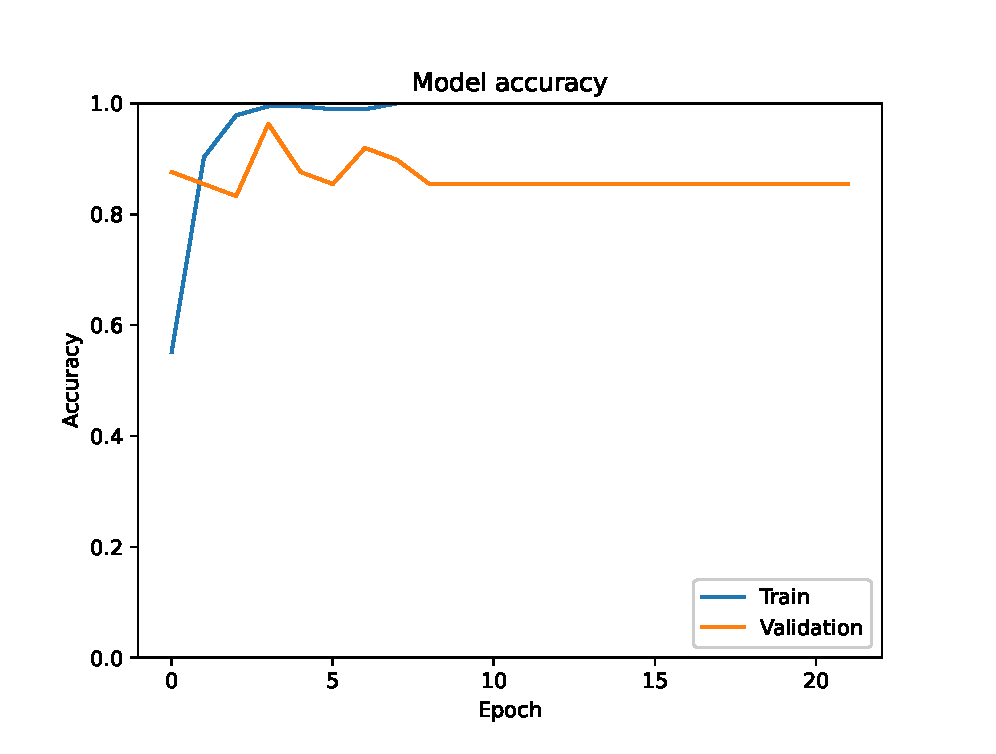
\includegraphics[width=\textwidth]{./fig/model3/accuracy3b.eps}
        \caption{Model-3b accuracy}
        \label{fig:model3b_acc}
    \end{minipage}
    \begin{minipage}{0.45\textwidth}
        \centering
        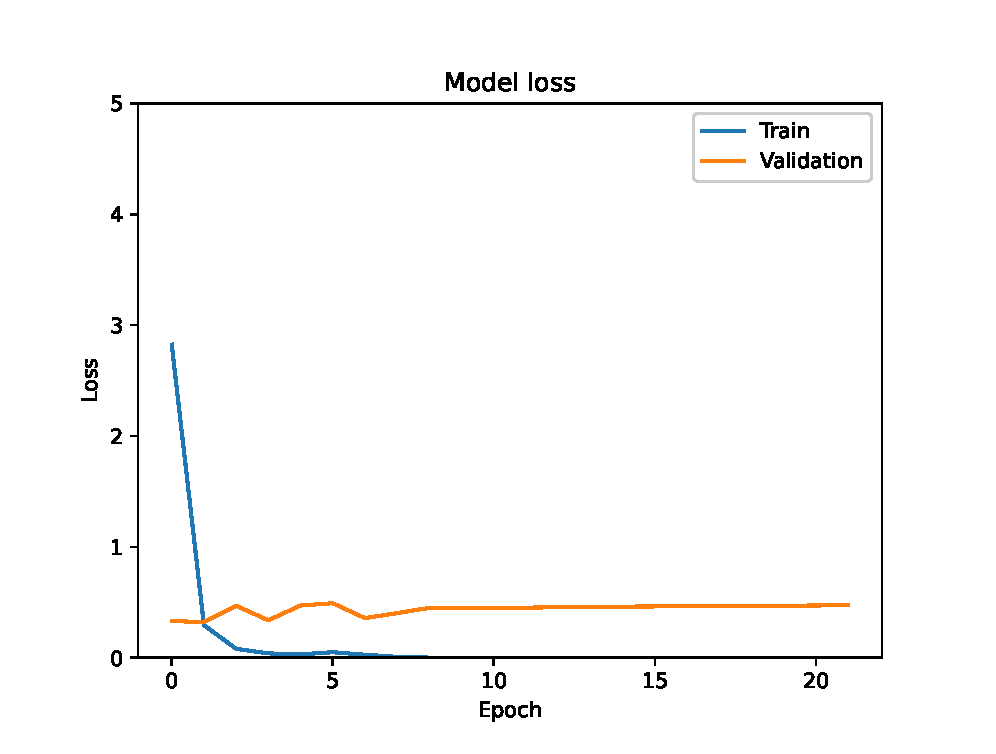
\includegraphics[width=\textwidth]{./fig/model3/loss3b.eps}
        \caption{Model-3b loss}
        \label{fig:model3b_loss}
    \end{minipage}
\end{figure}

\subsubsection{model 3c}
InceptionV3是一个相对于VGG16和VGG19更加复杂的模型,其在训练过程中引入了Inception模块,能够更好的提取图像的特征。其顶层的输入面积为299*299.
模型训练的准确度和损失如下\autoref{fig:model3c_acc}和\autoref{fig:model3c_loss}所示

\begin{figure}
    \centering
    \begin{minipage}{0.45\textwidth}
        \centering
        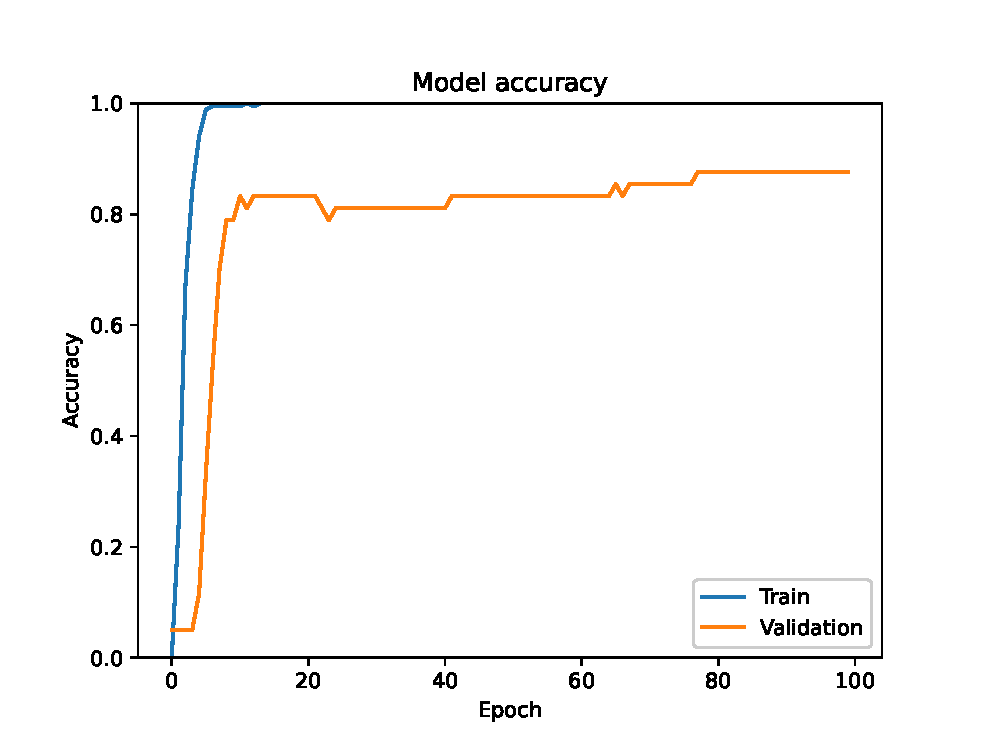
\includegraphics[width=\textwidth]{./fig/model3/accuracy3c.eps}
        \caption{Model-3c accuracy}
        \label{fig:model3c_acc}
    \end{minipage}
    \begin{minipage}{0.45\textwidth}
        \centering
        \includegraphics[width=\textwidth]{./fig/model3/loss3c.eps}
        \caption{Model-3c loss}
        \label{fig:model3c_loss}
    \end{minipage}
\end{figure}

注意到模型3c的验证准确度上依旧保持上升趋势,验证损失也在不断下降,这说明模型3c的训练可能还没到达最佳状态,模型欠拟合,需要进一步增加步长。

模型3d是对模型3c的改进,增加步长为1000(原来为100),模型训练的准确度和损失如\autoref{fig:model3d_acc}和\autoref{fig:model3d_loss}所示

\begin{figure}
        \centering
        \begin{minipage}{0.45\textwidth}
            \centering
            \includegraphics[width=\textwidth]{./fig/model3/accuracy3d.eps}
            \caption{Model-3d accuracy}
            \label{fig:model3d_acc}
        \end{minipage}
        \begin{minipage}{0.45\textwidth}
            \centering
            \includegraphics[width=\textwidth]{./fig/model3/loss3d.eps}
            \caption{Model-3d loss}
            \label{fig:model3d_loss}
        \end{minipage}
\end{figure}

\subsubsection{小结}

对比VGG16,VGG19和InceptionV3三个模型,可以发现InceptionV3的训练效果最好,其训练准确度和验证准确度收敛于1和0.9左右,损失收敛于0.5左右。这说明InceptionV3模型的训练效果最好,其泛化能力最强。

\subsection{模型选择总结}
横向对比模型1,模型2和模型3,可以发现模型3的训练效果最好。特别是模型3d。究其原因,可能是因为模型3是基于大规模图像识别的超深卷积网络,其在训练过程中能够更好的提取图像的特征,构建自己的特征空间。值得注意的是,模型3d,属于InceptionV3,在架构上具有模块化的设计,包括了多个“inception模块”。其包含了多尺度的卷积层,同时在同一层内并行运行。
在特征提取上,Inception模块可以在同一层内捕捉不同尺度的特征,使得网络能够自适应地选择更合适的特征表示。在处理深度上,InceptionV3利用批量标准化和残差连接来帮助训练深层网络,可以显著解决梯度消失的问题。

因此,我们选择模型3d作为我们的最终模型,用于后续的进一步应用和测试。


% \section{Presentation of experimental or analytical results/descriptions of final constructed product}

在这一部分,我们将讨论我们的模型的测试结果,并探索进一步改进的领域。

\subsection{在测试集上验证模型的准确性}

训练后,我们在一个特别准备的测试集上评估了模型的准确性。准确性定义为模型预测与实际标签匹配的样本比例。

下面的表格和图形展示了模型在不同类别中的准确性:

\begin{figure}[htbp]
    \centering
    \begin{minipage}{0.45\textwidth}
        \centering
        \captionof{table}{Model accuracy on test set}
        \begin{tabular}{cc}
            \toprule
            Category & Accuracy(\%) \\
            \midrule
            Normal & 98.4 \\
            Horizontal Line & 95.6 \\
            Vertical Line & 80.0 \\
            Slope & 96.1 \\
            Other & 95.2 \\
            \bottomrule
        \end{tabular}
        \label{tab:model_accuracy}
    \end{minipage}
    \begin{minipage}{0.45\textwidth}
        \centering
        \includegraphics[width=\textwidth]{./fig/assistplot/accuracy.eps}
        \captionof{figure}{Accuracy on Test Set}
        \label{fig:accuracy_histogram}
    \end{minipage}
\end{figure}


\textbf{模型性能分析}

模型在"正常"类别中的表现非常出色,准确率达到98.4%,这表明它在识别没有明显缺陷的组织切片方面具有强大的能力。同样,"水平线"和"其他"类别的准确度也很高,反映出模型在识别这些特定类型的缺陷方面的有效性。

然而,"垂直线"类别的准确度明显较低,只有80.0%。这表明模型识别这种类型缺陷的能力需要加强。这可能是由于训练数据不足,限制了模型的学习。也可能是因为垂直线的特征相对不太明显,使得模型难以准确提取特征。

\subsection{模型的改进(改变输入分辨率)}

在这里,我们将讨论模型进一步改进的可能性。

将高分辨率图像缩放到InceptionV3模型所需的默认大小299x299,确实可能导致信息和细节的丢失。这对于原始分辨率较高的图像尤其关键,例如VHX7000设备拍摄的2880x2160的图像。直接缩小这些图像可能会阻碍模型捕获所有微妙差异的能力,这在医学成像等细节丰富至关重要的领域尤其有害。

一种可能的解决方案是修改模型的输入层,以接受更大的图像尺寸。这种方法使模型能够处理更高分辨率的图像,从而保留更多的原始信息和细节,这可能会提高性能和准确度。InceptionV3架构,其具有多个不同核大小的卷积,特别适合处理更大的图像,因为它可以有效地捕获不同尺度的特征。

由于实验室硬件(16GB的显存)的限制,图像被缩放到原始大小的0.4倍,因此在这个实验中,图像的尺寸为1152x864。

\textbf{Training the New Model (Model 4)}

Model 4 is trained with these adjusted image sizes, and its training effectiveness is as follows:

\begin{figure}[H]
    \centering
    \begin{minipage}{0.45\textwidth}
        \centering
        \includegraphics[width=\textwidth]{./fig/model4/accuracy4.eps}
        \caption{Model-4 accuracy}
        \label{fig:model4_accuracy}
    \end{minipage}
    \begin{minipage}{0.45\textwidth}
        \centering
        \includegraphics[width=\textwidth]{./fig/model4/loss4.eps}
        \caption{Model-4 loss}
        \label{fig:model4_loss}
    \end{minipage}
\end{figure}

通过观察训练准确性和损失随时间的变化,我们可以看到模型性能有了显著的提升。训练和验证的准确性都接近1,验证损失降低到大约0.2,这表明模型具有强大的泛化能力。这表明模型不仅在训练数据上表现优秀,而且能够有效地泛化到新的、未见过的数据。

\textbf{在测试集上重新评估准确性}

更新后的模型然后在测试集上重新进行评估,结果如\autoref{tab:model_accuracy2}所示:

\begin{table}[H]
    \centering
    \caption{model accuracy on test set}
    \begin{tabular}{cccccc}
        \toprule
        & normal & horizental\_line & vertical\_line & slope & other \\
        \midrule
        accuracy(\%) & 98.4 & 96.7 & 85.6 & 96.5 & 96.5 \\
        \bottomrule
    \end{tabular}
    \label{tab:model_accuracy2}
    \end{table}

比较改变分辨率前后的准确性,有明显的提升,尽管不是很大。这种适度的增加可能归因于已经接近1的高准确性,进一步的改进有递减的回报。

结果证实了处理高分辨率图像的潜在好处,特别是在需要高保真和细节的设置中,如生物组织分析和研究。

\subsection{研究机器的最佳切割角度}

为了确定微切机的最佳切割角度,我们准备了在8到12度之间,以0.5度为增量的各种角度切割的组织切片图像。每个角度类别包含100个图像,总共有9个不同的数据组。然后使用模型4来评估每组的质量率,目标是找出获得高质量切片最多的角度。

下表和图形展示了每个切割角度的准确性,定义为高质量切割的百分比:

\begin{figure}[H]
    \centering
    \begin{minipage}{0.4\textwidth}
        \centering
        \captionof{table}{Normal accuracy on different angle}
        \begin{tabular}{cc}
            \toprule
            Angle & Accuracy(\%) \\
            \midrule
            8 & 80 \\
            8.5 & 81.5 \\
            9 & 83.5 \\
            9.5 & 93.3 \\
            10 & 96.6 \\
            10.5 & 88.8 \\
            11 & 84.2 \\
            11.5 & 66.6 \\
            12 & 62.2 \\
            \bottomrule
        \end{tabular}
        \label{tab:model_accuracy_angle}
    \end{minipage}
    \begin{minipage}{0.55\textwidth}
        \centering
        \includegraphics[width=\textwidth]{./fig/assistplot/angle_accuracy.eps}
        \captionof{figure}{Model Accuracy on Different Angle}
        \label{fig:angle_accuracy_histogram}
    \end{minipage}
\end{figure}

从\autoref{tab:model_accuracy_angle}中的数据可以看出,获得最高质量组织切片的最佳切割角度是10度,准确性高达96.6%。

此外,如\autoref{fig:angle_accuracy_histogram}所示,为了保持至少80%的切片质量率,切割角度应设置在9到10.5度之间。这个范围不仅确保了高质量切割的比率,而且还提供了一些机器设置的灵活性,以适应可能的组织类型或条件的变化。

\subsection{模型的泛化性}

到目前为止,实验已经使用了来自鱼类的卵巢组织切片。在实际应用中,我们可能会遇到各种各样的组织样本,包括其他器官或来自不同动物的标本。因此,评估我们的模型在各种组织类型上的泛化能力是至关重要的。

我们已经准备了一个新的数据集,包括鱼类肺部组织切片,分为四类:好、正常、差和其他。这些类别在下面的图中展示:(如\autoref{fig:fish_lung})

\begin{figure}[H]
    \centering
    \begin{minipage}{0.24\textwidth}
        \centering
        \includegraphics[width=\textwidth]{./fig/fish_lung/good20240313_144138.jpg}
        \caption*{Good}
        % \label{fig:good_fish_lung}
    \end{minipage}
    \begin{minipage}{0.24\textwidth}
        \centering
        \includegraphics[width=\textwidth]{./fig/fish_lung/normal20240313_141726.jpg}
        \caption*{Normal}
        % \label{fig:noraml_fish_lung}
    \end{minipage}
    \begin{minipage}{0.24\textwidth}
        \centering
        \includegraphics[width=\textwidth]{./fig/fish_lung/bad20240313_140952.jpg}
        \caption*{Bad}
        % \label{fig:bad_fish_lung}
    \end{minipage}
    \begin{minipage}{0.24\textwidth}
        \centering
        \includegraphics[width=\textwidth]{./fig/fish_lung/other20240313_141858.jpg}
        \caption*{Other}
        % \label{fig:other_fish_lung}
    \end{minipage}
    \caption{Four categories of fish lung tissue}
    \label{fig:fish_lung}
\end{figure}

保持原始的模型架构(模型4),但使用分辨率为1152x864的鱼肺图像重新训练。训练的准确性和损失在\autoref{fig:model5_acc}和\autoref{fig:model5_loss}中展示。
\begin{figure}[H]
    \centering
    \begin{minipage}{0.45\textwidth}
        \centering
        \includegraphics[width=\textwidth]{./fig/fish_lung/accuracy5.eps}
        \caption{Model-5 accuracy}
        \label{fig:model5_acc}
    \end{minipage}
    \begin{minipage}{0.45\textwidth}
        \centering
        \includegraphics[width=\textwidth]{./fig/fish_lung/loss5.eps}
        \caption{Model-5 loss}
        \label{fig:model5_loss}
    \end{minipage}
\end{figure}

训练和验证的准确性迅速增加并保持在高水平,表明模型在两个数据集上的性能都很强。损失图显示训练损失迅速下降到零,验证损失在初期的激增后稳定下来,这表明模型的拟合和泛化性都很好。

模型进一步在测试集上进行测试,结果显示在\autoref{fig:accuracy_histogram2}中。

\begin{figure}[H]
    \begin{minipage}{0.45\textwidth}
        \centering
        \captionof{table}{Model accuracy on test set}
        \begin{tabular}{ccccc}
            \toprule
            label & accuracy(\%) \\
            \midrule
            bad & 94.1 \\
            good & 98.2 \\
            normal & 94.7 \\
            other & 95.0 \\
            \bottomrule
        \end{tabular}
        \label{tab:model_accuracy3}
    \end{minipage}
    \begin{minipage}{0.45\textwidth}
        \centering
        \includegraphics[width=\textwidth]{./fig/assistplot/angle_accuracy2.eps}
        \caption{Accuracy on Test Set}
        \label{fig:accuracy_histogram2}
    \end{minipage}
\end{figure}

该模型在所有标签上的准确率超过90\%,表明其强大的性能和显著的泛化能力。这表明该模型可以有效地分类不同类型的组织切片,可能使其成为各种生物医学成像应用的多功能工具。 模型在不同组织类型上的稳健性强调了其在组织质量评估和分类任务中的潜力。

\FloatBarrier
% \section{Discussion and conclusions}
\label{sec:results}

\subsection{Discussion of results}


% 如上所述,这项研究旨在建立一个可靠的模型来分类组织切片图像。最初,我们实现了简单的CNN模型,但在观察到有限的成功后,研究转向了图像预处理,并最终确定了使用InceptionV3模型进行迁移学习,这产生了最好的结果。

% 值得注意的是,随着不同模型的试验,随着模型参数的调整或模型架构变得更复杂(如InceptionV3),模型的性能显著提高,即验证集的准确率变得更高,损失变得更低。

% 此外,比较模型系列1和2,我们发现使用预处理的图像来协助机器提取特征在图像分类任务中并不十分有效。图像处理可能导致重要细节和信息的丢失,从而影响机器的特征提取,进而影响模型的准确性和性能。

% 在第5节中,我们测试了模型的应用。首先,我们选择了一个额外的测试集来测试模型的准确性,并发现模型在所有测试集上的准确性都超过85\%。然后我们使用模型评估不同的切割角度,发现如果要保证切割质量在80\%以上,切割角度应在9度到10.5度之间。最后,我们使用了另一个鱼鳃切片图像的数据集进行二次验证,发现模型对测试集标签的预测准确性都在90\%以上,反映出该模型可以很好地应用于其他数据集。

% 下面展示的最终选定的模型配置,突显了我们在有效整合InceptionV3架构到训练框架中所采取的结构化方法。

如上所述,本研究旨在建立一个可靠的用于分类组织切片图像的模型。最初,我们实现了简单的CNN模型,但在观察到有限的成功后,研究转向了图像预处理,并最终选择了与InceptionV3模型一起使用的迁移学习,这产生了最好的结果。

值得注意的是,随着不同模型的试验,随着模型参数的调整或模型架构变得更复杂(如InceptionV3),模型的性能显著提高,即验证集的准确率变得更高,损失变得更低。

此外,比较模型系列1和2,我们发现使用预处理的图像来协助机器提取特征在图像分类任务中并不十分有效。图像处理可能会导致重要细节和信息的丢失,从而影响机器的特征提取,进而影响模型的准确性和性能。

在第5节中,我们测试了模型的应用。首先,我们选择了一个额外的测试集来测试模型的准确性,发现模型在所有测试集上的准确性都超过了85\%。然后我们使用模型来评估不同的切割角度,发现如果要保证切割质量在80\%以上,切割角度应在9度到10.5度之间。最后,我们使用了另一个鱼鳃切片图像的数据集进行二次验证,发现模型对测试集标签的预测准确性都在90\%以上,反映出该模型可以很好地应用于其他数据集。

下面展示的最终选择的模型配置,突出了我们如何有效地在训练框架中整合InceptionV3架构的结构化方法。
% \begin{center}

%     \begin{tikzpicture}[node distance=1.5cm,
%         box/.style={
%             rectangle,
%             rounded corners,
%             draw=black, very thick,
%             text width=15em,
%             minimum height=2em,
%             text centered},
%         arrow/.style={
%             thick,
%             ->,
%             >=stealth}
%         ]
    
%         \node (collect) [box] {输入层:1152*864};
%         \node (mix) [box, below of=collect] {基础模型:InceptionV3};
%         \node (train) [box, below of=mix] {全局平均池化层};
%         \node (test) [box, below of=train] {全连接层(节点个数取决于标签)-输出层};
%         \node (evaluate) [box, below of=test] {学习率:1e-4,优化器:Adam};
%         \node (rate) [box, below of=evaluate] {损失函数:交叉熵,评估指标:准确率};
%         \node (improve) [box, below of=rate] {早停:启用};
        
%         \draw [arrow] (collect) -- (mix);
%         \draw [arrow] (mix) -- (train);
%         \draw [arrow] (train) -- (test);
%         \draw [arrow] (test) -- (evaluate);
%         \draw [arrow] (evaluate) -- (rate);
%         \draw [arrow] (rate) -- (improve);
        
%         \end{tikzpicture}
% \end{center}
\begin{itemize}
    \item Input Layer: 1152*864
    \item Base Model: InceptionV3
    \item Global Average Pooling Layer
    \item Fully Connected Layer (Number of nodes based on Labels) - Output Layer
    \item Learning Rate: 1e-4, Optimizer: Adam
    \item Loss Function: Cross-Entropy, Performance Metric: Accuracy
    \item Early Stopping: Enabled
\end{itemize}

\subsection{Future work}
\subsubsection{提升分类方法}

当前的研究表明,现有的分类方法具有前景,但仅限于五个类别。通过扩大这些类别,我们可以增强我们对切割角度如何影响样本质量的理解,并提高我们分析的精度。更广泛的分类范围也会更好地预测各种组织类型和条件的最佳切割角度。采用更详细的分类可以促进向线性分析方法的转变,其中增加的类别作为离散点,使得通过线性回归准确建模切割角度和样本质量之间的关系成为可能。

线性判别分析(LDA)对于改进我们如何确定与组织质量相关的最佳切割角度特别有用。这种方法可以简化切割参数的预测,并改善对组织切割的控制。然而,过渡到线性判别框架带来了挑战。与输出概率的二元模型不同,线性回归模型需要变量(如切割角度和组织质量)之间有直接的相关性,这可能并非固有的线性。

此外,线性模型需要大量的数据,这可能会延长数据收集的时间,增加其复杂性,并需要更多的计算能力。当前使用TensorFlow和InceptionV3的系统已经在压榨GPU资源,突显了需要增强硬件的需求。这些进步,对于有效使用线性判别分析至关重要,将需要大量的时间和资源,以及进一步的理论和实践研究。例如,Jie Wen在"Robust Sparse Linear Discriminant Analysis"的工作中,将稀疏性整合到LDA模型中,使其更加健壮,适合复杂的应用\cite{6.1}。

\subsubsection{探究其他参数对切削质量的影响}

在之前的实验中,我们把切削角度设置为自变量,切削质量设置为因变量,建立了一个模型。然而,实际上切削质量可能受到其他参数的影响,如切削速度、给进速度(切片厚度)、刀具磨损等。

在将来的工作中,如果我们重点研究切削质量的影响因素,那么关于其他变量的研究将会是必须的。事实上,关于这些参数对质量的影响可以用一个函数来直观的表示:

\begin{equation}
    Q = f(\theta, v, f, w)
\end{equation}

其中,Q代表切削质量,$\theta$代表切削角度,v代表切削速度,f代表给进速度,w代表刀具磨损。至于这个函数里面的具体形式,也就是各个参数所占的权重,则需要大量的实验数据来统计然后拟合。这又将是一个挑战。


\subsubsection{性能提升和优化}

随着这项研究向大规模应用进展,性能优化成为了一个关键的挑战。这不仅涉及提高算法效率,还包括改善模型框架的可扩展性、稳定性和部署能力,以及优化底层编程语言和代码。

为了优化计算资源的使用,采用更高效的计算框架和并行处理算法是必要的。利用分布式计算资源可以显著减少模型训练时间,并在处理大型数据集时提高效率。此外,考虑到能耗和计算成本的限制,优化模型的计算架构和参数设置以在有限资源内最大化输出是至关重要的。

文章"TensorFlow和PyTorch在卷积神经网络中的应用效率分析"强调了TensorFlow和PyTorch在处理卷积神经网络时的差异\cite{6.2}。TensorFlow展示了较低的错误率和较小的收敛步骤,而PyTorch提供了更快的训练速度。

Pascal Fua的"Comparing Python, Go, and C++ on the N-Queens Problem"通过比较Python、Go和C++在解决N皇后问题上的效率,提出了优化深度学习性能的方法。\cite{6.3}研究发现,运行时语言在处理循环和数据流方面有明显优势,这表明编译工具如Numba、Cython和Pybind11可以在深度学习应用中提高性能。

\subsubsection{切割过程的优化}

我们的研究还发现,在切割过程中实时评估切片质量,并根据这些评估进行调整,可以显著提高组织切片的质量。

我们提出的反馈调整过程包括在显微切片机上方安装一个摄像头,捕获正在切割的样本的数据。这些数据然后由预训练的模型实时分析,评估切片的质量。基于这个评估,可以调整显微切片机的切割速度和角度参数,以提高后续切片的质量,从而确保可控和一致的样本质量。

实施这个系统面临几个挑战:

\begin{itemize} \item \textbf{实时图像处理:}需要一个清晰的摄像头和一个高效的实时图像处理系统,以快速捕获和处理图像数据。 \item \textbf{强大的计算资源:}需要一个预训练的模型和一个强大的计算机,以快速评估图像并根据评估调整显微切片机的参数。 \item \textbf{有效的控制接口:}需要一个高效的控制接口,以确保调整后的参数能及时传达给显微切片机。 \item \textbf{时间效率:}整个系统必须在切割间隔内操作。 \end{itemize}

一个相关的例子可以在研究"Convolutional neural networks applied to microtomy: Identifying the trimming-end cutting routine on paraffin-embedded tissue blocks"\cite{6.4}中找到。这项研究通过用摄像头监控切割过程,用CNN分析图像,并根据分析调整显微切片机的参数,自动化了切割过程。显微切片机、摄像头和深度学习模型的集成为在切割过程中实时评估和调整切割参数提供了一种可行的解决方案。

\subsection{Conclusions}

% 这项研究通过将深度学习技术应用于生物医学组织切片设备,显著推进了我们对优化活检参数的理解。通过采用复杂的卷积神经网络,特别是通过转移学习对InceptionV3模型的改造,该研究展示了一个能够高精度评估组织切片质量的强大框架。这种方法不仅提高了组织样本分析的准确性,而且引入了组织切片操作方法的范式转变。

% 通过评估不同角度的切片质量,我们发现了切割角度和切片质量之间的关系。这为我们提供了一种在未来提高切片质量的可行方法。此外,该模型在不同类型的组织(包括鱼卵巢和肺组织)中的应用,证实了其广泛的适应性和推广潜力,表明它适合各种组织切片和研究任务。

% 然而,该研究也突出了传统图像预处理技术的局限性。初步尝试通过图像预处理来提高模型性能并没有带来显著的改进,而在某些情况下,可能会模糊掉进行准确分类所必需的关键细节。这个发现表明,保持原始图像数据的完整性可能比应用激进的预处理技术更有益。

% 研究还探讨了通过扩展分类方法和优化性能来增强组织切片过程。这包括将更多的分类类别和线性分析方法如线性判别分析(LDA)结合进来,从而更精确地理解切割参数与样本质量之间的关系。同时,通过采用更高效的计算框架和并行处理技术来优化性能,以及探索额外参数如切割速度和进给率,都将提升模型的预测能力和组织切片的质量。此外,实施实时反馈系统,利用机器学习动态调整切割参数,将推动组织学制备向自动化迈进,确保更一致和高质量的组织切片。

% 总的来说,这个项目不仅展示了深度学习在生物医学研究和应用中的重要作用,而且为进一步改进组织切割技术提供了可行性。这些技术的结合可以为生物切割设备带来改进,提供一种可能的解决方案来提高组织样本的产出率和切割效率。这项研究为未来的组织切割技术提供了新的思路和方法,预计将在生物医学领域产生深远影响。


本研究通过将深度学习与生物医学组织切片设备相结合,显著增强了对优化活检参数的理解。该研究采用了通过迁移学习调整的InceptionV3模型,展示了一个用于高精度评估组织切片质量的强大框架。这种创新方法不仅提高了组织分析的准确性,而且革新了组织切片的操作方法。

研究发现了切割角度与组织切片质量之间的明显相关性,提供了一种实用的方法来提高未来切片的质量。模型在各种组织类型(如鱼卵巢和肺组织)上的有效性,突显了其广泛的适应性和广泛应用的潜力。

然而,研究也指出了传统图像预处理技术的局限性。初步的预处理并没有显著提高性能,有时甚至模糊了准确分类所需的关键细节。这表明,保留原始图像数据可能比应用广泛的预处理更有利。

本研究通过扩展分类方法和性能优化,提出了对组织切割过程的改进。这包括整合更多的分类类别和线性分析方法,如线性判别分析(LDA),以精细化理解切割参数与样本质量之间的关系。此外,探索影响切割质量的其他因素也是至关重要的。未来的工作将专注于优化计算框架和并行处理,以及检查其他参数,如切割速度和进给速率,以提高模型的预测性和组织切片的质量。预计实施一个使用机器学习动态调整切割参数的实时反馈系统,将推动组织学准备向全自动化发展,确保始终高质量的组织切片。

总的来说,这个项目不仅强调了深度学习在推进生物医学研究和应用中的关键作用,而且为组织切片技术的大幅改进奠定了基础。这些进步可能会显著提高组织样本处理的产量和效率,为未来组织切片技术的发展提供新的策略和方法,对生物医学产生持久的影响。



\FloatBarrier % Now the table doesn't flow over to any other sections

% %Conclusion


%%-----------English
% \pagenumbering{arabic}
\section{Introduction and background}
\label{sec:introduction}

\subsection{Background}

As the fundamental units of life, human research into cells and tissues has never ceased. Biological tissue sections, serving as crucial means for the direct observation of cellular morphology and structure, are essential for biomedical research and clinical diagnosis. A complete and usable tissue section is of great importance to researchers and physicians, as it provides vital information about cell structure, tissue morphology, and pathological changes. Within this, the quality of the section is of paramount importance.

Traditional manual sectioning methods are time-consuming and prone to variability, hence the emergence of automatic microtomes has provided a solution to these issues. For different biological tissues, varying cutting parameters can yield differing results, both positive and negative. Therefore, to enhance the utilization rate of biological sections and increase the production of high-quality specimens, determining optimal cutting parameters for specific tissues remains a goal.

Machine learning and deep learning have achieved significant success in the fields of computer vision and image processing. Machine learning is defined as a series of methods that can automatically detect patterns in data, which are then used to predict future outcomes or make decisions \cite{1.1}. In this paper, we integrate advanced image analysis and machine learning techniques to identify section quality and then evaluate the quality of tissue samples under different sectioning parameters.

\subsection{Introduction}

\textbf{Project Overview}

This project aims to optimize the cutting parameters of biological tissue microtomes, which are crucial devices in biomedical research and clinical diagnostics. The objective is to enhance the precision and efficiency of tissue sample preparation by determining the optimal slicing conditions. By collecting tissue samples under various cutting parameters and conducting subsequent manual image classification, this study employs deep learning techniques to analyze and predict the most effective cutting parameters. This work not only promises to improve the quality of tissue samples for microscopic examination but also helps to simplify laboratory workflows, thereby advancing biological and medical sciences.

\textbf{Objectives:}

\begin{enumerate}
    \item Collect a comprehensive dataset of tissue samples sliced under different parameters.
    \item Employ artificial image classification to categorize the quality and characteristics of these samples.
    \item Develop and train a deep learning model capable of assessing tissue sample quality.
    \item Use the model's insights to determine the optimal cutting parameters for the tissue slicer.
    \item Validate the model's predictions through empirical testing and refinement.
\end{enumerate}


\subsection{Structure of the Report}

The report is organized into multiple chapters, each focusing on specific aspects of the research on optimizing biopsy parameters using deep learning:

\textbf{Introduction and Background} - This initial chapter outlines the project's goals and framework, provides the motivation for the research, and describes the technical protocols and standards employed.

\textbf{Literature Review} - An extensive review of the relevant literature on biological tissue sections, image classification, and deep learning applications in biological sample preparation. This section contextualizes the current study within existing research.

\textbf{Methods and Theory} - A comprehensive description of the experimental methods, theoretical frameworks, and plans for data collection and processing.

\textbf{Experimental Work/Analysis Investigation/Design} - Details the experimental design, implementation, and analytical survey, explaining the strategies and methods used to meet the project objectives.

\textbf{Presentation of Experimental or Analysis Results/Final Constructed Product Description} - This chapter documents the experimental data, analysis results, or descriptions of the final design products, elaborating on the outcomes.

\textbf{Discussion and Conclusion} - Discusses the results in terms of their scientific significance and practical implications, draws conclusions, and suggests future research directions.

\textbf{Project Management, Sustainability, and Health Safety Considerations} - Covers project management strategies, addresses sustainability and health safety issues to ensure the research is conducted efficiently and safely.

\textbf{References} - Compiles all literature referenced throughout the research, supporting the study's foundation.


\textbf{Assumptions and Technical Specifications} - The project relies on several assumptions:

\begin{enumerate}
    \item Uniform properties of tissue samples across different batches.
    \item Reliability and accuracy of the biological tissue microtome and imaging equipment.
    \item Effectiveness of deep learning models in interpreting complex biological image data.
\end{enumerate}

Technical details regarding tissue microtome settings, image classification standards, and deep learning architecture are thoroughly described in the Methods and Theory section.

% \section{Literature review}

This literature review explores the integration of technologies in biological tissue sectioning, with a particular focus on the application of image classification and deep learning in optimizing slicing parameters. It aims to highlight significant advancements, identify gaps in current methodologies, and lay the groundwork for the proposed project.

\subsection{Microtome and Microscope Selection}

In recent years, the advent of automatic microtomes has significantly simplified the sectioning process and improved the quality of sections.

Zimmermann, in the article "Improved reproducibility in preparing precision-cut liver tissue slices," advocates for the use of the new Leica vibratome to enhance the accuracy and reproducibility of tissue sections from rats, mice, and human tissues \cite{LR.1}.

In this experiment, the HM355S microtome provided by Epredia is used for sectioning. This machine is a popular device for biological tissue sectioning research, and many experiments and papers have utilized this equipment for sectioning.

Elzbieta Klimuszko has used the HM355S microtome for sectioning teeth to investigate the calcium and magnesium content in dental enamel \cite{LR.2}.

Andelko Hrzenjak also used the HM355S microtome for sectioning pathological endometrial tissues to study the mechanisms of endometrial carcinoma development \cite{LR.3}.

Similarly, the choice of microscope is crucial. In this experiment, the VHX7000 microscope from Keyence is used for image acquisition. It is capable of capturing images of biological tissue sections (e.g., mouse prostate cells \cite{LR.4}),
as well as inorganic materials (such as ceramics \cite{LR.5}, glass \cite{LR.6}).

The experiments will employ the HM355s microtome and VHX7000 microscope for sectioning and image acquisition. This setup ensures that both equipment selection and technological application are optimally aligned to enhance the precision and efficiency of the tissue sectioning process, supporting the overall goals of the research project.

% 近年来,自动切片机的出现显著简化了切片过程,并提高了切片的质量。

% Zimmermann在文章"Improved reproducibility in preparing precision-cut liver tissue slices"中,主张使用新的Leica振动刀来提高大鼠、小鼠和人体组织切片的精度和重复性 \cite{LR.1}。

% 在这个实验中,我们使用Epredia提供的HM355S切片机进行切片。这台机器是生物组织切片研究的流行设备,许多实验和论文都使用了这台设备进行切片。

% Elzbieta Klimuszko使用HM355S切片机切割牙齿,以研究牙釉质中的钙和镁含量 \cite{LR.2}。

% Andelko Hrzenjak也使用HM355S切片机切割病理性子宫内膜组织,以研究子宫内膜癌发展的机制 \cite{LR.3}。

% 同样,显微镜的选择也至关重要。在这个实验中,我们使用Keyence的VHX7000显微镜进行图像采集。它能够捕获生物组织切片的图像(例如,小鼠前列腺细胞 \cite{LR.4}),以及无机材料(如陶瓷 \cite{LR.5},玻璃 \cite{LR.6})。

% 实验将使用HM355s切片机和VHX7000显微镜进行切片和图像采集。这种设置确保了设备选择和技术应用的最佳配合,以提高组织切片过程的精度和效率,支持研究项目的总体目标。

\subsection{Deep Learning in Tissue Sectioning}

The application of deep learning technologies in the biomedical field has achieved significant advancements. Deep learning models excel in tasks such as image classification, object detection, and segmentation, providing powerful tools for research and diagnostics in biomedical laboratories.

Lorena Guachi-Guachi proposed a method utilizing CNN networks to identify and refine tissue sections. This approach represents an innovative application of deep learning that can enhance the precision of tissue preparation and analysis \cite{LR.7}.

In the book \textit{Biomedical Texture Analysis}, Vincent Andrearczyk introduced a CNN architecture specifically designed for texture analysis, which significantly improves the accuracy of classifying biological tissues compared to traditional architectures \cite{LR.8}. This development demonstrates the potential of deep learning to enhance the detailed analysis of tissue characteristics, which is crucial for accurate diagnostics and research.

Yan Xu suggested that features extracted from CNNs trained on the large natural image database, ImageNet, can be transferred to histopathological images of tissues. This provides a viable approach for implementing transfer learning, which can greatly enhance the efficiency of tissue image classification and analysis \cite{LR.9}.

Based on the literature, deep learning technology holds broad prospects for application in image classification and analysis of tissue sections. By leveraging deep learning models, efficient identification and classification of tissue samples can be achieved, providing strong support for optimizing sectioning parameters.

This section underscores the transformative impact of deep learning on the field of tissue sectioning, promising significant improvements in the accuracy and utility of histological analyses.

% 在生物医学领域,深度学习技术的应用已取得了显著的进步。深度学习模型在图像分类、对象检测和分割等任务中表现出色,为生物医学实验室的研究和诊断提供了强大的工具。

% Lorena Guachi-Guachi 提出了一种利用 CNN 网络识别和精炼组织切片的方法。这种方法代表了深度学习的创新应用,可以提高组织准备和分析的精度 \cite{LR.7}。

% 在《生物医学纹理分析》一书中,Vincent Andrearczyk 介绍了一种专为纹理分析设计的 CNN 架构,与传统架构相比,这种架构显著提高了生物组织分类的准确性 \cite{LR.8}。这一发展展示了深度学习提高组织特性详细分析的潜力,这对于准确的诊断和研究至关重要。

% Yan Xu 提出,从在大型自然图像数据库 ImageNet 上训练的 CNN 中提取的特征可以转移到组织的病理学图像上。这为实施转移学习提供了一种可行的方法,可以大大提高组织图像分类和分析的效率 \cite{LR.9}。

% 根据文献,深度学习技术在组织切片的图像分类和分析中有广阔的应用前景。通过利用深度学习模型,可以实现组织样本的有效识别和分类,为优化切片参数提供了强大的支持。

% 这一部分强调了深度学习对组织切片领域的变革性影响,预示着在组织学分析的准确性和实用性方面的显著改进。



% \section{Methodology and theory}
\label{sec:problem_description}

\subsection{Experimental Workflow}

The experiment workflow is outlined in the diagram below, detailing the sequential steps from data collection to iterative improvement of the model.

\begin{center}
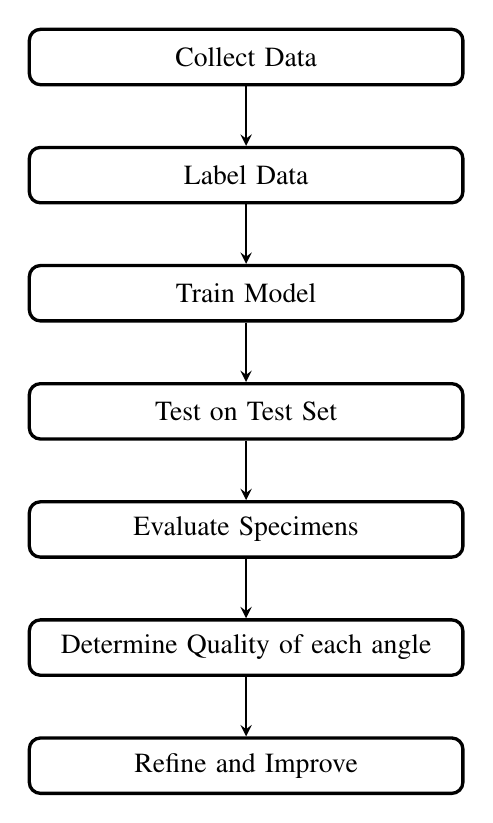
\begin{tikzpicture}[node distance=1.5cm,
    box/.style={
        rectangle,
        rounded corners,
        draw=black, very thick,
        text width=15em,
        minimum height=2em,
        text centered},
    arrow/.style={
        thick,
        ->,
        >=stealth}
    ]

    \node (collect) [box] {Collect Data};
    \node (mix) [box, below of=collect] {Label Data};
    \node (train) [box, below of=mix] {Train Model};
    \node (test) [box, below of=train] {Test on Test Set};
    \node (evaluate) [box, below of=test] {Evaluate Specimens};
    \node (rate) [box, below of=evaluate] {Determine Quality of each angle};
    \node (improve) [box, below of=rate] {Refine and Improve};
    
    \draw [arrow] (collect) -- (mix);
    \draw [arrow] (mix) -- (train);
    \draw [arrow] (train) -- (test);
    \draw [arrow] (test) -- (evaluate);
    \draw [arrow] (evaluate) -- (rate);
    \draw [arrow] (rate) -- (improve);
    
    \end{tikzpicture}
\end{center}

\textbf{Data Collection:} Utilize a microtome to slice tissue sections that have been pre-prepared and paraffin-embedded in a biological laboratory following staining procedures. Operate the microtome according to its manual to obtain images of the sections and record the cutting parameters.

\textbf{Data Labeling:} Label the collected image data based on the quality of the sections and their suitability for biological observation and analysis.

\textbf{Model Training:} Experiment with various structures and forms of deep learning convolutional models to train the labeled data. Monitor accuracy and loss functions during the training process to assess model performance.

\textbf{Testing with Test Set:} Evaluate the trained model using a test set to assess its generalization capability.

\textbf{Specimen Evaluation:} Assess an additional prepared test set to observe the practical application effects of the model, calculating the model’s prediction accuracy.

\textbf{Determination of Cutting Yield:} Use pre-prepared image data of sections cut at different angles to evaluate with the model, deriving the yield of good cuts at various angles to determine the optimal cutting angle.

\textbf{Improvements and Enhancements:} Based on the evaluation results, adjust and enhance the model to improve its accuracy and generalization capabilities.

\subsection{Image Processing Methods}

For the acquired image data, appropriate image preprocessing can be applied. Under the premise of maintaining the integrity and quality of images, certain processing can be implemented to highlight the features intended for computer recognition and, to some extent, remove irrelevant features and noise. This enhances the accuracy of subsequent deep learning models.

Image segmentation is a critical step in image processing, aiming to divide the image into several meaningful regions for further analysis and processing. In models focusing on the yield rate of biological tissues, it is necessary to segment the biological sections into biological tissue and paraffin areas, emphasizing the biological tissue parts.

Common image segmentation algorithms include edge detection and threshold segmentation.

\subsubsection{Edge Detection for Tissue Slices}
For biological tissue sections, a crucial indicator of quality is the clarity of the section's edges. The integrity and continuity of the slice edges can reflect whether there are quality issues with the sample.

There are numerous algorithms for edge detection, such as Sobel, Laplacian, and Canny operators \cite{3.1}.

The \textbf{Sobel operator} is a first-order differential operator that can be used to detect image edges \cite{补充1}. Suppose there is a one-dimensional image $f(x)$, the relationship between its intensity and the pixel coordinate $x$ can be represented as shown in Figure 1. It can be observed in \autoref{fig:original_function} that the slope is the largest around x=2.2, indicating that there is a sudden change in image intensity (an edge exists) near this point. Taking its derivative gives the first-order derivative $f'(x)$, as shown in \autoref{fig:first_derivative}, where the absolute value of the derivative is the largest. The Sobel operator uses this characteristic to detect edges.

\begin{figure}[htbp]
    \centering
    \begin{minipage}[b]{0.32\textwidth}
        \centering
        \includegraphics[width=\textwidth]{./fig/original_function.png}
        \caption{f(x)}
        \label{fig:original_function}
    \end{minipage}
    \begin{minipage}[b]{0.32\textwidth}
        \centering
        \includegraphics[width=\textwidth]{./fig/first_derivative.png}
        \caption{f'(x)}
        \label{fig:first_derivative}
    \end{minipage}
    \begin{minipage}[b]{0.32\textwidth}
        \centering
        \includegraphics[width=\textwidth]{./fig/second_derivative.png}
        \caption{f''(x)}
        \label{fig:second_derivative}
    \end{minipage}
\end{figure}

The \textbf{Laplacian operator} is a second-order differential operator that performs well in edge detection of images. It is derived by taking the derivative of the Sobel operator once more. In 2D images, the Laplacian operator is defined as follows: 

\begin{equation} 
    \nabla^2 f = \frac{\partial^2 f}{\partial x^2} + \frac{\partial^2 f}{\partial y^2} 
\end{equation} 

As shown in the figure above, taking the derivative of the first-order derivative results in the second-order derivative $f''(x)$, as shown in \autoref{fig:second_derivative}. It can be seen that around x=2.2, the second-order derivative is 0, which indicates that when the value of the Laplacian operator $\nabla^2 f$ is 0, there is a sudden change in image intensity, indicating the presence of an edge.

\textbf{Canny Operator} is a multi-stage differential operator that enhances the edge detection process by incorporating noise suppression, building on the initial computations similar to those used by the Sobel operator. Introduced by John F. Canny in 1986 \cite{3.2}, the Canny operator refines the results obtained from Sobel operator calculations through additional steps such as non-maximum suppression and hysteresis thresholding. These steps set thresholds to eliminate false edges from the image, resulting in more accurate edge detection.

In the section on "Experimental Work/Analytical Investigation/Design", experiments will be conducted on the collected image data using these three edge detection algorithms—Sobel, Laplacian, and Canny—to compare their effectiveness. This comparative analysis will help in identifying the most suitable method for edge detection in the context of tissue sectioning, where the clarity and precision of edges are vital for quality assessment. The results will guide the selection of the optimal algorithm to be integrated into the image processing pipeline, enhancing the capability of the system to accurately segment and analyze biological tissue sections.

\subsubsection{Theresold Segmentation for Tissue Slices}

Apart from edge detection, another method employed is threshold segmentation. This technique divides the image pixels into two categories: those above a certain threshold and those below it. It is particularly useful in situations where there is a significant grayscale difference between the target and the background in the image.

For specimens, a straightforward approach is to contrast the colors of the paraffin area and the biological tissue area (which is stained during preparation), and then separate them using threshold segmentation. Assuming the biological tissue is yellow and the paraffin is white, setting a threshold could isolate the white parts of the image, leaving behind the biological tissue.

Additionally, there are more sophisticated methods of threshold segmentation, such as the Otsu method used for fingerprint extraction. Implementing this method can significantly enhance the segmentation of biological tissues. Yue Yaru and Zhu Jialin in "Algorithm of fingerprint extraction and implementation based on OpenCV" have proposed an improved Otsu-based fingerprint extraction algorithm using OpenCV. This algorithm excels particularly under conditions of uneven illumination and blurred images, providing accurate, simple, and fast fingerprint extraction \cite{3.3}.

Comparisons and experiments related to these segmentation techniques will be conducted in the "Experimental Work/Analytical Investigation/Design" section.

\subsection{Simple Convolutional Neural Network Framework}

Based on the design of convolutional neural network architectures discussed in the literature review, a simple convolutional neural network framework is suitable for classifying images of biological tissue sections in this project. We have constructed three simple convolutional neural network models, labeled as configurations a, b, and c.

Each of these models features a distinct combination of convolutional layers and neuron numbers in both the convolutional and fully connected layers, as summarized in the table below:

\begin{table}[H]
    \centering
    \caption{Configuration of the simple CNN model}
    \begin{tabular}{ccccc}
        \toprule
        \textbf{Layer Type} & \textbf{Configuration a} & \textbf{Configuration b} & \textbf{Configuration c} \\
        \midrule
        Input Layer & - & - & - \\
        Conv Layer 1 & Conv3-32 (relu) & Conv3-16 (relu) & Conv3-32 (relu) \\
        Pooling Layer 1 & MaxPooling & MaxPooling& MaxPooling \\
        Conv Layer 2 & Conv3-32 (relu) & Conv3-32 (relu) & Conv3-32 (relu) \\
        Pooling Layer 2 & MaxPooling & MaxPooling& MaxPooling \\
        Conv Layer 3 & Conv3-32 (relu) & Conv3-64 (relu) & Conv3-32 (relu) \\
        Pooling Layer 3 & MaxPooling & MaxPooling& MaxPooling \\
        Flattening Layer & Flatten() & Flatten() & Flatten() \\
        FC(Full connect) & Dense(128, relu) & Dense(128, relu) & Dense(256, relu) \\
        Output Layer & - & - & - \\
        \bottomrule
    \end{tabular}
    \label{tab:cnn_simple_configuration}
    \end{table}

Model a consists of three convolutional layers with 32 neurons each and a fully connected layer with 128 neurons. Model b features three convolutional layers with a progressively increasing number of neurons (16, 32, and 64), and a fully connected layer with 128 neurons. Model c also includes three convolutional layers, each with 32 neurons, but differs in its fully connected layer, which contains 256 neurons.

The primary differences among these models lie in the number of neurons in the convolutional and fully connected layers. In the "Experimental Work/Analytical Investigation/Design" section, these models will be subjected to experiments and performance evaluations to compare their effectiveness.

\subsection{Model Selection of Transfer Learning Methods}
In transfer learning, commonly used pre-trained models include VGG16, VGG19, Inception, and others. These models have been extensively trained on large datasets like ImageNet, where the weights of various layers in the model have been optimized and can be effectively used for transfer learning\cite{4.30 7}.

\autoref{tab:model_comparison} displays the number of parameters for models such as the VGG series (VGG16, VGG19) designed by the Visual Geometry Group at the University of Oxford \cite{DL.5}, as well as the modular deep learning models InceptionV3 \cite{DL.6}\cite{DL.7} developed by Google. These models possess a vast quantity of parameters, enabling them to accurately extract features from complex images. Utilizing the capabilities of these well-trained models allows researchers and practitioners to achieve high performance on specific tasks without the need to train the entire network from scratch, thereby saving time and resources while maintaining high accuracy\cite{4.30 8}.

\begin{table}[H]
    \centering
    \caption{Comparison of Transfer Learning Models}
    \label{tab:model_comparison}
    \begin{tabular}{cccc}
        \toprule
        \textbf{Model} & \textbf{VGG16} & \textbf{VGG19} & \textbf{InceptionV3}\\
        \midrule
        \textbf{Number of Parameters} & 138,357,544 & 143,667,240 & 23,851,784 \\
        \bottomrule
    \end{tabular}
\end{table}

The primary differences between these models are as follows:

\begin{itemize}
\item VGG16 (Model 3a) and VGG19 (Model 3b) are similar, but VGG19 includes three additional convolutional layers, potentially offering better feature extraction capabilities.
\item InceptionV3 (Model 3c) incorporates Inception modules, enabling it to capture a broader range of features across multiple scales, providing a more complex and possibly more effective feature extraction mechanism.
\end{itemize}

Considering that these models are all trained on the ImageNet dataset, and the features of the biological tissue slice dataset are quite different from the ImageNet dataset. As for how to determine the best model, it needs to be verified through experiments. In the section of "Experimental Work/Analytical Investigation/Design", these models will be experimented and performance evaluated, comparing their effects.






 
% \section{Experimental work/ analytical investigation/ design}

\textbf{Experimental workflow}

The experiment workflow is outlined in the diagram below, detailing the sequential steps from data collection to iterative improvement of the model.

\begin{center}

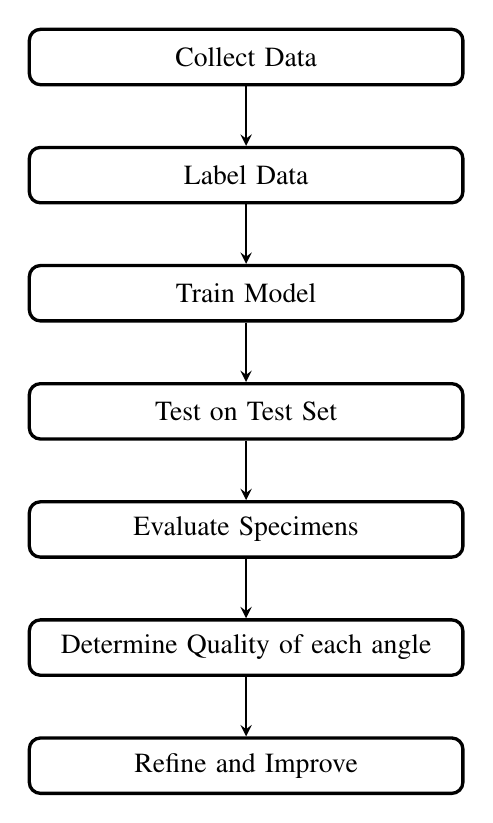
\begin{tikzpicture}[node distance=1.5cm,
    box/.style={
        rectangle,
        rounded corners,
        draw=black, very thick,
        text width=15em,
        minimum height=2em,
        text centered},
    arrow/.style={
        thick,
        ->,
        >=stealth}
    ]

    \node (collect) [box] {Collect Data};
    \node (mix) [box, below of=collect] {Label Data};
    \node (train) [box, below of=mix] {Train Model};
    \node (test) [box, below of=train] {Test on Test Set};
    \node (evaluate) [box, below of=test] {Evaluate Specimens};
    \node (rate) [box, below of=evaluate] {Determine Quality of each angle};
    \node (improve) [box, below of=rate] {Refine and Improve};
    
    \draw [arrow] (collect) -- (mix);
    \draw [arrow] (mix) -- (train);
    \draw [arrow] (train) -- (test);
    \draw [arrow] (test) -- (evaluate);
    \draw [arrow] (evaluate) -- (rate);
    \draw [arrow] (rate) -- (improve);
    
    \end{tikzpicture}
\end{center}



\subsection{Data Collection}
The first essential step for deep learning is data collection. In this experiment, pre-prepared paraffin-embedded tissue sections (fish ovary tissues) were used. These sections were placed on an HM355s automatic microtome, and slicing operations were performed according to different cutting angles as specified in the microtome's manual. The cutting data was recorded meticulously.

%在这不要提三个点的鱼的肺泡组织,在后面作为模型二次验证和增强使用。

The schematic diagram of the microtome (taking a tooth as an example) is shown in \autoref{fig:cutting_machine} \cite{4.1}.

\begin{figure}[htbp]
    \centering
    \begin{minipage}{0.48\textwidth}
        \centering
        \includegraphics[width=\textwidth]{./fig/machine.jpg}
        \caption{Microtome}
        \label{fig:machine}
    \end{minipage}
    \begin{minipage}{0.48\textwidth}
        \centering
        \includegraphics[width=\textwidth]{./fig/10266_2018_353_Fig1_HTML.jpg}
        \caption{Working principle of the microtome}
        \label{fig:cutting_machine}
    \end{minipage}
\end{figure}
% https://link.springer.com/article/10.1007/s10266-018-0353-6



% 在切削过程中,从切角为8度开始(如\autoref{fig:machine}中的angle of inclination),每次增加0.5度,直到切角为12度。切片机在切片过程中保持给进速度为25,厚度为1。

In the experiment, the microtome was configured with the following parameters: the mode was set to continuous, the feed rate was 5.0, the trimming value was 25, the speed was set at 32, the water flow rate was 7.5, and the water temperature was approximately 36 degrees Celsius. The cutting angle was adjusted between 8 to 12 degrees.

The biological tissues used for sectioning are shown in Figure \ref{label:sample}. After sectioning, the different types of tissue sections were placed on slides as depicted in Figure \ref{fig:采集样本}. Once dried, these slides were transferred under a VHX7000 microscope for imaging. Each sample was photographed under the microscope to capture electronic image data, as shown in Figure \ref{fig:显微镜}.

\begin{figure}[htbp]
    \centering
    \begin{minipage}{0.3\textwidth}
        \centering
        \includegraphics[width=\textwidth]{./fig/sample.jpg}
        \caption{Biological tissues}
        \label{label:sample}
    \end{minipage}
    \begin{minipage}{0.3\textwidth}
        \centering
        \includegraphics[width=\textwidth]{./fig/采集样本.jpg}
        \caption{Collecting samples}
        \label{fig:采集样本}
    \end{minipage}
    \begin{minipage}{0.35\textwidth}
        \centering
        \includegraphics[width=\textwidth]{./fig/显微镜.jpg}
        \caption{Microscope}
        \label{fig:显微镜}
    \end{minipage}
\end{figure}


Based on this, several hundred images were obtained, each with a resolution of 2880*2160. An example of the samples is shown in \autoref{fig:sample9.5}.


\begin{figure}
    \centering
    \includegraphics[width=0.8\textwidth]{./fig/sample9.5.jpg}
    \caption{Sample with a cutting angle of 9.5 degrees}
    \label{fig:sample9.5}
\end{figure}


\subsection{Data Labeling}

For this experiment, the dataset is re-labeled based on the quality of the tissue sections. Overall, the quality of the biological tissues is categorized into two primary classes: normal and bad. Further analysis of the collected data revealed common flaws - the presence of vertical or horizontal white creases on the sections, which clearly indicate unusable slices. Given the distinct nature of these flaws, they are classified into two additional specific categories: \textbf{horizontal line}(\autoref{fig:horizental_line}) and \textbf{vertical line}(\autoref{fig:vertical_line}).

\begin{figure}[H]
    \centering
    \begin{minipage}{0.45\textwidth}
        \centering
        \includegraphics[width=\textwidth]{./fig/sample_1/horizental_line.jpg}
        \caption{horizental line}
        \label{fig:horizental_line}
    \end{minipage}
    \begin{minipage}{0.45\textwidth}
        \centering
        \includegraphics[width=\textwidth]{./fig/sample_1/vertical_line.jpg}
        \caption{vertical line}
        \label{fig:vertical_line}
    \end{minipage}
\end{figure}

Additionally, some images were noted to have a significant rotational angle at the time of sampling. These instances are categorized separately as \textbf{slope}(\autoref{fig:slope}). Finally, any images that do not fit into the aforementioned categories but still show irregularities(Excessive changes in brightness) are labeled as \textbf{other}(\autoref{fig:other}). 

\begin{figure}[H]
    \centering
    \begin{minipage}{0.45\textwidth}
        \centering
        \includegraphics[width=\textwidth]{./fig/sample_1/slope.jpg}
        \caption{slope}
        \label{fig:slope}
    \end{minipage}
    \begin{minipage}{0.45\textwidth}
        \centering
        \includegraphics[width=\textwidth]{./fig/sample_1/other.jpg}
        \caption{other}
        \label{fig:other}
    \end{minipage}
\end{figure}

An example of a normal slice that meets observational requirements is shown in \autoref{fig:normal}.

\begin{figure}[H]
    \centering
    \begin{minipage}{0.45\textwidth}
        \centering
        \includegraphics[width=\textwidth]{./fig/sample_1/normal.jpg}
        \caption{normal}
        \label{fig:normal}
    \end{minipage}
\end{figure}


For each image, we need to label it as one of the above five categories. This will serve as our dataset for training the model.


\FloatBarrier

\subsection{Model 1: Original Images with a Simple CNN Network}

For a new dataset, where the appropriate complexity of the model for the given image complexity is uncertain, a basic CNN architecture is initially employed to gauge the characteristics of the dataset and the complexity of the images.

\begin{table}[H]
\centering
\caption{Configuration of the simple CNN model}
\begin{tabular}{ccccc}
    \toprule
    \textbf{Layer Type} & \textbf{Configuration 1a} & \textbf{Configuration 1b} & \textbf{Configuration 1c} \\
    \midrule
    Input Layer & - & - & - \\
    Conv Layer 1 & Conv3-32 (relu) & Conv3-16 (relu) & Conv3-32 (relu) \\
    Pooling Layer 1 & MaxPooling & MaxPooling& MaxPooling \\
    Conv Layer 2 & Conv3-32 (relu) & Conv3-32 (relu) & Conv3-32 (relu) \\
    Pooling Layer 2 & MaxPooling & MaxPooling& MaxPooling \\
    Conv Layer 3 & Conv3-32 (relu) & Conv3-64 (relu) & Conv3-32 (relu) \\
    Pooling Layer 3 & MaxPooling & MaxPooling& MaxPooling \\
    Flattening Layer & Flatten() & Flatten() & Flatten() \\
    FC(Full connect) & Dense(128, relu) & Dense(128, relu) & Dense(256, relu) \\
    Output Layer & - & - & - \\
    \bottomrule
\end{tabular}
\label{tab:cnn_simple_configuration}
\end{table}

The configurations of the simple CNN models used are outlined in \autoref{tab:cnn_simple_configuration}. These initial models, labeled as Configuration 1a, 1b, and 1c, vary in terms of the number of neurons in the convolutional layers and the size of the neurons in the fully connected layers. Configuration 1a and 1b differ by the number of neurons in the convolutional layers, whereas Configuration 1c differs from Configuration 1a in the size of the neurons in the fully connected layer.

The preprocessing steps involve splitting the dataset into training (80\%) and testing (20\%) sets. In the input layer, the image dimensions are halved (from 2880x2160 to 1440x1080), and the data is normalized.

During training, the Adam optimizer and cross-entropy loss function are used, with early stopping implemented to avoid overfitting.

The graphs below display the accuracy and loss of Models 1a, 1b, and 1c over the training epochs.

\begin{figure}[H]
    \centering
    \begin{minipage}{0.49\textwidth}
        \centering
        \includegraphics[width=\textwidth]{./fig/model1/accuracy11.eps}
        \caption{Accuracy of Model 1}
        \label{fig:model11_acc}
    \end{minipage}
    \begin{minipage}{0.49\textwidth}
        \centering
        \includegraphics[width=\textwidth]{./fig/model1/loss11.eps}
        \caption{Loss of Model 1}
        \label{fig:model11_loss}
    \end{minipage}
\end{figure}


From the charts, it is observed that Models 1a, 1b, and 1c exhibit a gradual increase in training accuracy, stabilizing over time, while training losses decrease, approaching zero. This indicates that the models are learning from the training data relatively well. However, for the validation set, the accuracy of all three models stabilizes within the range of 80\% to 85\%, and the validation loss is comparatively high in some cases, especially with Model 1a, where it approaches 2.5 and shows significant fluctuations. This suggests a degree of overfitting, where the models perform better on the training data than on unseen data. Notably, Model 1c shows the best performance in terms of validation loss, indicating that its structure or parameter adjustments may be more effective at improving generalization.

The likely cause of overfitting here could be the insufficient complexity of the models relative to the complexity of the dataset, indicating that the models may not be effectively extracting features from the data. Although the models achieve high accuracy and low losses on the training set, their generalization capabilities on the validation set need enhancement.

To improve model accuracy, considering preprocessing of the images and assisting the model with feature extraction manually might be beneficial, helping the model better generalize to new data.

\FloatBarrier


\subsection{Image Preprocessing Improvement}

In cases where model performance is suboptimal, it may be due to the complexity of the images which hampers the model's ability to extract significant features effectively. Therefore, image preprocessing techniques such as edge detection and threshold segmentation are considered to highlight desired features for recognition by the model and to reduce irrelevant features and noise, thereby improving the accuracy of subsequent deep learning models.


\subsubsection{Edge Detection}

As mentioned in section 3.1.1, the principle of edge detection involves identifying changes in pixel intensity (gradients) to determine edges within an image. Assuming the original image is displayed in \autoref{fig:sample9.5}.

Before proceeding with edge detection, an initial preprocessing step—Gaussian blur—is applied. The rationale behind Gaussian blurring is that it helps reduce noise in the image, smoothens the gradient transitions, and decreases the likelihood of detecting false edges, thus enhancing the accuracy of edge detection\cite{4.3}. We experiment with Gaussian kernels of sizes 21, 41, 61, and 81, which correspond to 1\%, 2\%, 3\%, and 4\% of the image width, respectively.

The images post-Gaussian blurring are displayed below. To better demonstrate the impact of the Gaussian kernel size on edge detection, the Sobel operator is used post-blurring to compute edges and increase brightness by 50 units for visibility.

\begin{figure}
    \centering
    \begin{minipage}{0.45\textwidth}
        \centering
        \includegraphics[width=\textwidth]{./fig/gausssian/blurred21.jpg}
        \caption{blurred k=21}
        \label{fig:blurred21}
    \end{minipage}
    \begin{minipage}{0.45\textwidth}
        \centering
        \includegraphics[width=\textwidth]{./fig/gausssian/sobel21.jpg}
        \caption{sobel k=21}
        \label{fig:sobel21}
    \end{minipage}
\end{figure}

\begin{figure}
    \centering
    \begin{minipage}{0.45\textwidth}
        \centering
        \includegraphics[width=\textwidth]{./fig/gausssian/blurred41.jpg}
        \caption{blurred k=41}
        \label{fig:blurred41}
    \end{minipage}
    \begin{minipage}{0.45\textwidth}
        \centering
        \includegraphics[width=\textwidth]{./fig/gausssian/sobel41.jpg}
        \caption{sobel k=41}
        \label{fig:sobel41}
    \end{minipage}
\end{figure}

\begin{figure}
    \centering
    \begin{minipage}{0.45\textwidth}
        \centering
        \includegraphics[width=\textwidth]{./fig/gausssian/blurred61.jpg}
        \caption{blurred k=61}
        \label{fig:blurred61}
    \end{minipage}
    \begin{minipage}{0.45\textwidth}
        \centering
        \includegraphics[width=\textwidth]{./fig/gausssian/sobel61.jpg}
        \caption{sobel k=61}
        \label{fig:sobel61}
    \end{minipage}
\end{figure}

\begin{figure}
    \centering
    \begin{minipage}{0.45\textwidth}
        \centering
        \includegraphics[width=\textwidth]{./fig/gausssian/blurred81.jpg}
        \caption{blurred k=81}
        \label{fig:blurred81}
    \end{minipage}
    \begin{minipage}{0.45\textwidth}
        \centering
        \includegraphics[width=\textwidth]{./fig/gausssian/sobel81.jpg}
        \caption{sobel k=81}
        \label{fig:sobel81}
    \end{minipage}
\end{figure}

From \autoref{fig:blurred21} to \autoref{fig:blurred81}, it can be observed that as the Gaussian blur kernel size increases, the image details become progressively more blurred, and the edges also become more indistinct. From \autoref{fig:sobel21} to \autoref{fig:sobel81}, the effectiveness of edge detection diminishes as the kernel size increases, with the edges becoming less prominent. Considering the clarity of image edges against background noise, a Gaussian kernel size of 61 is selected.


Following the application of Gaussian blur (k=61), the results using the Laplacian operator via Python's OpenCV library are depicted below:

\begin{figure}[H]
\centering
\includegraphics[width=0.45\textwidth]{./fig/gausssian/laplacian61.jpg}
\caption{Result of applying the Laplacian operator}
\label{fig:laplacian}
\end{figure}

As previously mentioned, the Canny algorithm is more sophisticated compared to the Sobel algorithm, incorporating steps such as thresholding and non-maximum suppression. The Canny method uses two thresholds, a low and a high. An image gradient greater than the high threshold is marked as an edge, while a gradient below the low threshold is not considered an edge. Gradients that are between the two thresholds are only considered edges if they are connected to high-threshold edges, effectively reducing noise and resulting in more accurate edge detection.

Typically, the ratio between the high and low thresholds is between 2:1 and 3:1. For this experiment, a ratio of 2.5:1 is selected, and the impact of different thresholds on edge detection is explored.

The chosen low thresholds are 2, 4, and 6, with corresponding high thresholds of 5, 10, and 15, respectively. The results of the Canny algorithm are shown below:

\begin{figure}[H]
    \centering
    \begin{minipage}{0.45\textwidth}
        \centering
        \includegraphics[width=\textwidth]{./fig/gausssian/canny61+2.jpg}
        \caption{Canny thresholds 2 and 5}
        \label{fig:canny2_5}
    \end{minipage}
    \begin{minipage}{0.45\textwidth}
        \centering
        \includegraphics[width=\textwidth]{./fig/gausssian/canny61+4.jpg}
        \caption{Canny thresholds 4 and 10}
        \label{fig:canny4_10}
    \end{minipage}
\end{figure}

\begin{figure}[H]
    \centering
    \begin{minipage}{0.45\textwidth}
        \centering
        \includegraphics[width=\textwidth]{./fig/gausssian/canny61+6.jpg}
        \caption{Canny thresholds 6 and 15}
        \label{fig:canny6_15}
    \end{minipage}
\end{figure}

Among the three Canny results, \autoref{fig:canny4_10} exhibits the best performance, managing to retain most of the edge details while effectively eliminating most of the noise. Consequently, the thresholds of 4 and 10 are chosen for the Canny algorithm.

\textbf{Summary}

Comparing the results of the Sobel, Laplacian, and Canny algorithms, the Sobel algorithm shows average performance, with significant edge detection but limited noise reduction. The Laplacian algorithm performs the worst, with edges becoming nearly invisible, likely due to its high sensitivity to noise. The Canny algorithm delivers the best results, maintaining edge details while effectively removing most noise. Therefore, the Canny algorithm is selected as the method for image preprocessing, enhancing the model's ability to focus on relevant features for further analysis.

\FloatBarrier


\subsubsection{Threshold Segmentation}

Considering the distinct colors of the biological tissue samples (yellow) and paraffin (white) in the specimens, threshold segmentation offers a straightforward method to distinguish between these two components by isolating the white regions of the image, leaving the biological tissue intact. This procedure involves enhancing the image contrast and saturation to better highlight the yellow color of the biological tissues, as demonstrated in \autoref{fig:enhanced_image}. The processing steps are executed using Python's OpenCV library.

Initially, each pixel in the image is evaluated, and pixels within approximately a radius of 15 (about 1\% of the image width) surrounding yellow pixels are preserved. Other colors are removed, as shown in \autoref{fig:yellowpic}. However, this method has shown limitations due to the dispersal of tissue fragments during the sectioning process, which can appear scattered throughout the specimen and interfere with the detection of yellow pixels.

\begin{figure}[H]
    \centering
    \begin{minipage}{0.45\textwidth}
        \centering
        \includegraphics[width=\textwidth]{./fig/threshold/enhanced_image.jpg}
        \caption{Enhanced image for better color differentiation}
        \label{fig:enhanced_image}
    \end{minipage}
    \begin{minipage}{0.45\textwidth}
        \centering
        \includegraphics[width=\textwidth]{./fig/threshold/yellowpic.jpg}
        \caption{Segmentation focused on yellow pixels}
        \label{fig:yellowpic}
    \end{minipage}
\end{figure}

To refine the segmentation, further processing is required to eliminate black blocks appearing in the image. This is achieved by applying a mask inversion to turn these black blocks into white, thereby enhancing the separation of biological tissue from the paraffin base. The results are displayed in \autoref{fig:mask}.

\begin{figure}[H]
    \centering
    \begin{minipage}{0.45\textwidth}
        \centering
        \includegraphics[width=\textwidth]{./fig/threshold/final.jpg}
        \caption{Final image after removing black blocks}
        \label{fig:mask}
    \end{minipage}
    \begin{minipage}{0.45\textwidth}
        \centering
        \includegraphics[width=\textwidth]{./fig/threshold/fingerprint.jpg}
        \caption{Result of segmentation using the fingerprint algorithm}
        \label{fig:fingerprint}
    \end{minipage}
\end{figure}

This approach demonstrates the utility of combining color enhancement and thresholding techniques to effectively segment biological tissue from paraffin in microscopic images. The challenge lies in accurately distinguishing tissue fragments from background noise and other non-tissue elements. This method can be particularly effective for automated image analysis in histopathology, where accurate tissue segmentation is crucial for research.

\subsubsection{Another Threshold Segmentation Method: Fingerprint Algorithm}
During the literature review, an article was found that described an improved segmentation method based on the Otsu algorithm, specifically adapted for fingerprint segmentation. Considering that both tissue sections and fingerprints are biological tissues with complex patterns and textures, it was hypothesized that this algorithm might also be effective for segmenting tissue sections. The results of applying this method are illustrated in \autoref{fig:fingerprint}.

The fingerprint algorithm, which is an adaptation of the Otsu method, is particularly effective in differentiating areas of high and low density, which is ideal for applications like fingerprint recognition where contrast between ridges and valleys is critical. The use of this algorithm in the context of biological tissue segmentation may offer a robust way to delineate regions of different cellular densities or structures within a sample.

\subsubsection*{Summary}

Based on the image preprocessing techniques discussed, both edge detection and threshold segmentation have shown promising results in highlighting the features of biological tissues and eliminating interference from paraffin. These preprocessing steps have significantly enhanced the visibility of essential features while minimizing noise and irrelevant information, which is critical for accurate analysis in histopathology.

To leverage these improvements, three datasets can be established:

\begin{itemize}
    \item Images processed through \textbf{edge detection.}
    \item Images processed through \textbf{threshold segmentation.}
    \item Images processed using \textbf{the fingerprint algorithm.}
\end{itemize}

These datasets will serve as training sets for the upcoming model training phase. Utilizing diverse preprocessing approaches not only enhances model robustness by providing varied representations of the data but also helps in exploring which image preprocessing technique best assists the model in learning relevant features effectively.
\FloatBarrier



\subsection{Model 2: Preprocessed Images with a Simple CNN Network}

In this section, we adapt Model 1c, the best-performing model from the previous experiments, to utilize preprocessed images. The architecture remains unchanged; however, the input now consists of images that have undergone various preprocessing techniques:

\begin{itemize}
    \item \textbf{Model 2a:} Utilizes images processed with Canny edge detection.
    \item \textbf{Model 2b:} Uses images processed through threshold segmentation.
    \item \textbf{Model 2c:} Inputs are images segmented using the fingerprint algorithm.
\end{itemize}

Each model follows the same architecture as Model 1c, which includes three convolutional layers each with 32 feature maps and 3x3 kernels, max pooling layers, and a fully connected layer with 256 neurons.

Results are displayed in the graphs below(\autoref{fig:model22_acc} and \autoref{fig:model22_loss}), showcasing the training and validation accuracy and loss for Models 2a, 2b, and 2c.
\begin{figure}
    \centering
    \begin{minipage}{0.49\textwidth}
        \centering
        \includegraphics[width=\textwidth]{./fig/model2/accuracy22.eps}
        \caption{Accuracy of Model 2}
        \label{fig:model22_acc}
    \end{minipage}
    \begin{minipage}{0.49\textwidth}
        \centering
        \includegraphics[width=\textwidth]{./fig/model2/loss22.eps}
        \caption{Loss of Model 2}
        \label{fig:model22_loss}
    \end{minipage}
\end{figure}


\subsubsection*{Summary}
The graphs illustrate that Models 2a and 2c begin to stabilize after approximately 8 training epochs, with training accuracies nearing 100\%, while validation accuracies stabilize around 65\% and 75\%, respectively. Despite high accuracies, both models exhibit relatively high validation losses above 1, suggesting overfitting and limited generalization to unseen data.

Model 2b, however, converges after about 10 training epochs, displaying the highest validation accuracy at approximately 82\% and a lower loss fluctuating between 1 and 1.2. This indicates that Model 2b performs better on the validation set, suggesting better adaptability and robustness. This might be due to Model 2b processing color images, which provide richer features from RGB channels, potentially enhancing feature extraction and generalization capabilities.

However, there is a risk that important details could be lost in the preprocessing steps, particularly with Model 2b's threshold segmentation. This can negatively affect the model's performance on specific types of images. An example of this loss of key information is demonstrated below:

\begin{figure}
    \centering
    \begin{minipage}{0.45\textwidth}
        \centering
        \includegraphics[width=\textwidth]{./fig/model2/origin20240205_161427.jpg}
        \caption{Original Image}
        \label{fig:origin}
    \end{minipage}
    \begin{minipage}{0.45\textwidth}
        \centering
        \includegraphics[width=\textwidth]{./fig/model2/yellow20240205_161427.jpg}
        \caption{Image after Yellow Threshold Segmentation}
        \label{fig:yellow}
    \end{minipage}
\end{figure}

In \autoref{fig:yellow}, we see that the threshold segmentation algorithm used in Model 2b’s training set significantly enhances horizontal creases, potentially confusing the model during training.

These findings highlight the challenges in image preprocessing. Aggressive preprocessing can sometimes eliminate crucial information, leading to diminished training outcomes. In future steps, transfer learning might be employed, utilizing pre-trained large-scale deep learning models adapted to our dataset, to improve training effectiveness and address these challenges.


\subsection{Model 3: Original Images with Transfer Learning}

\textbf{Transfer Learning with Pre-trained Models}
We are incorporating three well-known models pre-trained on the ImageNet dataset: VGG16, VGG19, and InceptionV3. These models come with pre-trained weights that are highly optimized and are expected to improve feature extraction capabilities significantly when adapted to our specific dataset.

\begin{itemize}
    \item VGG16 (Model 3a) and VGG19 (Model 3b) are similar, with VGG19 having three additional convolutional layers that could potentially offer better feature extraction capabilities.
    \item InceptionV3 (Model 3c) incorporates Inception modules that allow it to capture a broader range of features at multiple scales, providing a more complex and possibly more effective feature extraction mechanism.
\end{itemize}

\textbf{Adaptations for Transfer Learning}

To prevent overfitting and optimize the transfer learning process:

\begin{itemize}
    \item Early stopping is utilized.
    \item Learning rates are set low, at 1e-5 for VGG16 and VGG19, and slightly higher at 1e-4 for InceptionV3, given its more complex architecture.
    \item All models are adapted to accept an input size of 224x224, except for InceptionV3 which uses its default input size of 299x299. This uniform input size helps standardize the data preprocessing step.
    \item A global average pooling layer is added to each model following the base model layers, followed by a fully connected layer that matches the number of output classes.
\end{itemize}


\textbf{Observations from Model Training}

The training and validation performance of these models is depicted below:

\begin{figure}[H]
    \centering
    \begin{minipage}{0.49\textwidth}
        \centering
        \includegraphics[width=\textwidth]{./fig/model3/accuracy33.eps}
        \caption{Accuracy of Model 3}
        \label{fig:model33_acc}
    \end{minipage}
    \begin{minipage}{0.49\textwidth}
        \centering
        \includegraphics[width=\textwidth]{./fig/model3/loss33.eps}
        \caption{Loss of Model 3}
        \label{fig:model33_loss}
    \end{minipage}
\end{figure}

\textbf{Analysis}
\begin{itemize}
    \item Models 3b (VGG19) and 3c (InceptionV3) show significantly higher validation accuracies around 90\%, compared to Model 3a (VGG16).
    \item The loss metrics indicate that Model 3c (InceptionV3) has the lowest validation loss among the three, suggesting it is the most effective in generalizing to unseen data. This underscores InceptionV3's superior capability in capturing complex features.
    \item The performance gap between Model 3a and Model 3b supports the notion that the additional convolutional layers in VGG19 enhance its ability to process image features more effectively than VGG16.
\end{itemize}


\subsubsection*{Summary}

A comparative analysis of the VGG16, VGG19, and InceptionV3 models reveals that InceptionV3 yields the best training results, with both training and validation accuracies converging around 1 and 0.9 respectively, and losses converging around 0.6. This indicates that the InceptionV3 model not only trains effectively but also demonstrates superior generalization capabilities.

\subsection{Model Selection Summary}
When comparing across the model series—Model 1, Model 2, and Model 3—it is evident that Model 3 performs the best, particularly Model 3c. The underlying reason is likely due to Model 3's foundation on deep convolutional networks that are pre-trained on large-scale image datasets, enabling more effective feature extraction and development of a robust feature space.

\textbf{Notable Attributes of Model 3c (InceptionV3):}

\begin{itemize}
    \item \textbf{Architectural Design:} InceptionV3 features a modular design incorporating multiple "inception modules," which include multi-scale convolutional layers that operate in parallel within the same layer. This modular approach allows the network to capture a broad spectrum of features at various scales and depths.
    \item \textbf{Feature Extraction:} Inception modules can adaptively capture appropriate feature representations by processing different scales of features within the same layer. This adaptability makes it exceptionally capable of handling complex image data like biomedical images.
    \item \textbf{Deep Network Handling:} InceptionV3 integrates batch normalization and residual connections, which are critical in training deep networks. These techniques effectively mitigate issues related to vanishing gradients, thus facilitating the training of deeper models without performance degradation.
\end{itemize}

Given these advantages, Model 3c (InceptionV3) is selected as our final model for further applications and testing. This model stands out not only for its advanced architectural innovations but also for its proven effectiveness in generalizing well to new, unseen data, making it highly suitable for complex tasks such as medical image analysis where accuracy and reliability are paramount.


% \section{Presentation of Experimental or Analytical Results/Descriptions of Final Constructed Product}

In this section, we discuss the testing outcomes of our models and explore areas for further improvement.

\subsection{Validating Model Accuracy on a Test Set}

After training, the models were evaluated on a specially prepared test set to measure their accuracy. The accuracy is defined as the proportion of samples for which the model's predictions match the actual labels.

The table and figure below present the accuracy of the model across different categories:

\begin{figure}[H]
    \centering
    \begin{minipage}{0.45\textwidth}
        \centering
        \captionof{table}{Model Accuracy on Test Set}
        \begin{tabular}{cc}
            \toprule
            Category & Accuracy(\%) \\
            \midrule
            Normal & 98.4 \\
            Horizontal Line & 95.6 \\
            Vertical Line & 80.0 \\
            Slope & 96.1 \\
            Other & 95.2 \\
            \bottomrule
        \end{tabular}
        \label{tab:model_accuracy}
    \end{minipage}
    \begin{minipage}{0.45\textwidth}
        \centering
        \includegraphics[width=\textwidth]{./fig/assistplot/accuracy.eps}
        \captionof{figure}{Accuracy on Test Set}
        \label{fig:accuracy_histogram}
    \end{minipage}
\end{figure}

\textbf{Analysis of Model Performance}
The model performs exceptionally well for the 'Normal' category with an accuracy of 98.4\%, indicating its robust capability in identifying tissue sections without significant defects. Similarly, high accuracy scores are noted for 'Horizontal Line' and 'Other' categories, reflecting the model’s effectiveness in recognizing these specific types of imperfections.

However, the accuracy for the "Vertical Line" category is significantly lower, at 80.0\%. This indicates that the model's ability to recognize this type of defect needs to be strengthened. This could be due to insufficient training data, which limits the model's learning. It could also be because the features of vertical lines are relatively less obvious, making it difficult for the model to accurately extract features.

\subsection{Improvement of the Model (Changing Input Resolution)}

Here we discuss the potential for further improvement of the model.

Rescaling high-resolution images to the default size of 299x299, as required by the InceptionV3 model, can indeed result in the loss of information and detail. This is particularly crucial for images originally at much higher resolutions, such as those captured by the VHX7000 device at 2880x2160. Directly scaling down these images may hinder the model's ability to capture all subtle differences, which is especially detrimental in fields like medical imaging where detail richness is paramount.

One potential solution is to modify the model's input layer to accept larger image sizes. This approach allows the model to process higher resolution images, thus retaining more original information and detail, which could lead to improved performance and higher accuracy. The InceptionV3 architecture, with its multiple convolutions of varying kernel sizes, is particularly well-suited to handle larger images as it can capture features at different scales effectively.

Due to the limitations imposed by the lab's hardware (16GB of VRAM), the images are rescaled to 0.4 times their original size, resulting in dimensions of 1152x864 for this experiment.

\textbf{Training the New Model (Model 4)}

Model 4 is trained with these adjusted image sizes, and its training effectiveness is as follows:

\begin{figure}[H]
    \centering
    \begin{minipage}{0.45\textwidth}
        \centering
        \includegraphics[width=\textwidth]{./fig/model4/accuracy4.eps}
        \caption{Accuracy of Model 4}
        \label{fig:model4_accuracy}
    \end{minipage}
    \begin{minipage}{0.45\textwidth}
        \centering
        \includegraphics[width=\textwidth]{./fig/model4/loss4.eps}
        \caption{Loss of Model 4}
        \label{fig:model4_loss}
    \end{minipage}
\end{figure}

Observations of training accuracy and loss over time indicate a significant improvement in model performance. Both training and validation accuracies approach 1, with validation losses dropping to around 0.2, suggesting strong generalization capabilities. This indicates that the model not only excels on training data but can also generalize effectively to new, unseen data.

\textbf{Re-Evaluating Accuracy on the Test Set}

The updated model is then re-evaluated on the test set, with results as \autoref{tab:model_accuracy2}:

\begin{table}[H]
    \centering
    \caption{Model 4 accuracy on the test set}
    \begin{tabular}{cccccc}
        \toprule
        & normal & horizental\_line & vertical\_line & slope & other \\
        \midrule
        accuracy(\%) & 98.4 & 96.7 & 85.6 & 96.5 & 96.5 \\
        \bottomrule
    \end{tabular}
    \label{tab:model_accuracy2}
    \end{table}

Comparing the accuracy before and after changing the resolution, there is a noticeable improvement, though it is not substantial. This modest increase could be attributed to the already high accuracies nearing 1, where further improvements have diminishing returns.

The results affirm the potential benefits of processing higher-resolution images, particularly in settings demanding high fidelity and detail, such as biological tissue analysis and research.

\subsection{Investigating the Optimal Cutting Angle for the Machine}

In order to determine the optimal cutting angle for the microtome, images of tissue sections cut at various angles ranging from 8 to 12 degrees, at 0.5-degree increments, were prepared. Each angle category consisted of 100 images, resulting in a total of 9 distinct groups of data. Model 4 was then utilized to assess the quality rate of each group, aiming to identify the angle at which the highest yield of quality sections was achieved.

The table and graph below present the accuracy, defined as the percentage of high-quality cuts, for each cutting angle:

\begin{figure}[H]
    \centering
    \begin{minipage}{0.4\textwidth}
        \centering
        \captionof{table}{Normal accuracy on different angles}
        \begin{tabular}{cc}
            \toprule
            Angle & Accuracy(\%) \\
            \midrule
            8 & 80 \\
            8.5 & 81.5 \\
            9 & 83.5 \\
            9.5 & 93.3 \\
            10 & 96.6 \\
            10.5 & 88.8 \\
            11 & 84.2 \\
            11.5 & 66.6 \\
            12 & 62.2 \\
            \bottomrule
        \end{tabular}
        \label{tab:model_accuracy_angle}
    \end{minipage}
    \begin{minipage}{0.55\textwidth}
        \centering
        \includegraphics[width=\textwidth]{./fig/assistplot/angle_accuracy.eps}
        \captionof{figure}{Model Accuracy on Different Angle}
        \label{fig:angle_accuracy_histogram}
    \end{minipage}
\end{figure}

From the data presented in \autoref{tab:model_accuracy_angle}, it is evident that the optimal cutting angle for achieving the highest yield of quality tissue sections is 10 degrees, which demonstrates an impressive 96.6\% accuracy.

Additionally, as illustrated in \autoref{fig:angle_accuracy_histogram}, to maintain a section quality rate of at least 80\%, the cutting angle should be set between 9 and 10.5 degrees. This range not only ensures a high rate of quality cuts but also offers some flexibility in machine settings to accommodate possible variations in tissue type or condition.


\subsection{Model Generalizability}

The experiments thus far have utilized ovarian tissue sections from fish. In practical applications, we may encounter diverse tissue samples, including other organs or specimens from different animals. Therefore, it's crucial to assess the generalizability of our model across various tissue types.

A new dataset comprising fish lung tissue sections has been prepared, categorized into four classes: good, normal, bad, and other. These categories are demonstrated in the figures below:
(as shown in \autoref{fig:fish_lung})


\begin{figure}[H]
    \centering
    \begin{minipage}{0.24\textwidth}
        \centering
        \includegraphics[width=\textwidth]{./fig/fish_lung/good20240313_144138.jpg}
        \caption*{Good}
        % \label{fig:good_fish_lung}
    \end{minipage}
    \begin{minipage}{0.24\textwidth}
        \centering
        \includegraphics[width=\textwidth]{./fig/fish_lung/normal20240313_141726.jpg}
        \caption*{Normal}
        % \label{fig:noraml_fish_lung}
    \end{minipage}
    \begin{minipage}{0.24\textwidth}
        \centering
        \includegraphics[width=\textwidth]{./fig/fish_lung/bad20240313_140952.jpg}
        \caption*{Bad}
        % \label{fig:bad_fish_lung}
    \end{minipage}
    \begin{minipage}{0.24\textwidth}
        \centering
        \includegraphics[width=\textwidth]{./fig/fish_lung/other20240313_141858.jpg}
        \caption*{Other}
        % \label{fig:other_fish_lung}
    \end{minipage}
    \caption{Four categories of fish lung tissue}
    \label{fig:fish_lung}
\end{figure}

The original model architecture (Model 4) is maintained but retrained with the fish lung images at a resolution of 1152x864. The training accuracy and loss are presented in the \autoref{fig:model5_acc} and \autoref{fig:model5_loss}.

\begin{figure}[H]
    \centering
    \begin{minipage}{0.45\textwidth}
        \centering
        \includegraphics[width=\textwidth]{./fig/fish_lung/accuracy5.eps}
        \caption{Accuracy of Model 5}
        \label{fig:model5_acc}
    \end{minipage}
    \begin{minipage}{0.45\textwidth}
        \centering
        \includegraphics[width=\textwidth]{./fig/fish_lung/loss5.eps}
        \caption{Loss of Model 5}
        \label{fig:model5_loss}
    \end{minipage}
\end{figure}

The training and validation accuracy rapidly increase and maintain high levels, indicating robust model performance on both datasets. The loss plot shows a rapid decline in training loss towards zero, with validation loss stabilizing after an initial spike—suggesting good fit and generalization.

The model is further tested on a test set, and the results are shown in \autoref{fig:accuracy_histogram2}.

\begin{figure}[H]
    \begin{minipage}{0.45\textwidth}
        \centering
        \captionof{table}{Model accuracy on the test set}
        \begin{tabular}{ccccc}
            \toprule
            label & accuracy(\%) \\
            \midrule
            bad & 94.1 \\
            good & 98.2 \\
            normal & 94.7 \\
            other & 95.0 \\
            \bottomrule
        \end{tabular}
        \label{tab:model_accuracy3}
    \end{minipage}
    \begin{minipage}{0.45\textwidth}
        \centering
        \includegraphics[width=\textwidth]{./fig/assistplot/angle_accuracy2.eps}
        \caption{Accuracy on Test Set}
        \label{fig:accuracy_histogram2}
    \end{minipage}
\end{figure}

The model demonstrates over 90\% accuracy across all labels, indicating its strong performance and substantial generalizability. This suggests that the model can effectively classify different types of tissue sections, potentially making it a versatile tool for various biomedical imaging applications.
The robustness of the model across different tissue types underscores its potential in tissue quality assessment and classification tasks.


% \section{Discussion and conclusions}
\label{sec:results}

\subsection{Discussion of results}

As detailed above, this research aimed to establish a reliable model for classifying tissue section images. Initially, simple CNN models were implemented, but upon observing limited success, the study shifted towards image preprocessing and finally settled on transfer learning with the InceptionV3 model, which produced the best results.

It is worth noting that with the trial of different models, as the model parameters are adjusted or the model architecture becomes more complex (such as InceptionV3), the model's performance significantly improves, i.e., the accuracy of the validation set becomes higher and the loss becomes lower.

Furthermore, comparing model series 1 and 2, we found that using preprocessed images to assist the machine in extracting features is not very effective in the task of image classification. Image processing may lead to the loss of important details and information, thereby affecting the machine's feature extraction, and thus affecting the accuracy and performance of the model.

In Section 5, we tested the model in application. First, we selected an additional test set to test the model's accuracy and found that the model's accuracy on all test sets was greater than 85\%. Then we used the model to evaluate different cutting angles and found that if the cutting quality is to be guaranteed at 80\%, the cutting angle should be between 9 degrees and 10.5 degrees. Finally, we used another dataset of fish alveolar slice images for secondary verification and found that the model's prediction accuracy for the test set labels was all above 90\%, reflecting that the model can be well applied to other datasets.

The Final selected model configuration, showed below, highlights the structured approach taken to integrate the InceptionV3 architecture effectively within the training framework.

% \begin{center}

%     \begin{tikzpicture}[node distance=1.5cm,
%         box/.style={
%             rectangle,
%             rounded corners,
%             draw=black, very thick,
%             text width=15em,
%             minimum height=2em,
%             text centered},
%         arrow/.style={
%             thick,
%             ->,
%             >=stealth}
%         ]
    
%         \node (collect) [box] {Input Layer: 1152*864};
%         \node (mix) [box, below of=collect] {Base Model: InceptionV3};
%         \node (train) [box, below of=mix] {Global Average Pooling Layer};
%         \node (test) [box, below of=train] {Fully Connected Layer (Nodes based on Labels) - Output Layer};
%         \node (evaluate) [box, below of=test] {Learning Rate: 1e-4, Optimizer: Adam};
%         \node (rate) [box, below of=evaluate] {Loss Function: Cross-Entropy, Performance Metric: Accuracy};
%         \node (improve) [box, below of=rate] {Early Stopping: Enabled};
        
%         \draw [arrow] (collect) -- (mix);
%         \draw [arrow] (mix) -- (train);
%         \draw [arrow] (train) -- (test);
%         \draw [arrow] (test) -- (evaluate);
%         \draw [arrow] (evaluate) -- (rate);
%         \draw [arrow] (rate) -- (improve);
        
%         \end{tikzpicture}
% \end{center}
\begin{itemize}
    \item Input Layer: 1152*864
    \item Base Model: InceptionV3
    \item Global Average Pooling Layer
    \item Fully Connected Layer (Number of nodes based on Labels) - Output Layer
    \item Learning Rate: 1e-4, Optimizer: Adam
    \item Loss Function: Cross-Entropy, Performance Metric: Accuracy
    \item Early Stopping: Enabled
\end{itemize}

\subsection{Future work}

\subsubsection{Enhancing Classification Methods}

Current research indicates that existing classification methods are promising but limited to five categories. By expanding these categories, we could enhance our understanding of how cutting angles impact sample quality and improve the precision of our analyses. A broader classification range would also better predict optimal cutting angles for various tissue types and conditions. Adopting a more detailed classification could facilitate a shift to linear analytical methods, where increased categories serve as discrete points, enabling accurate modeling of relationships between cutting angles and sample quality through linear regression.

Linear Discriminant Analysis (LDA) is particularly useful for refining how we determine optimal cutting angles in relation to tissue quality. This method could simplify the prediction of cutting parameters and improve control over tissue sectioning. However, transitioning to a linear discriminant framework introduces challenges. Unlike binary models that output probabilities, linear regression models require a direct correlation between variables like cutting angles and tissue quality, which might not be inherently linear.

Furthermore, linear models demand significantly more data, which can prolong data collection, increase its complexity, and require more computational power. Current systems using TensorFlow and InceptionV3 are already straining GPU resources, highlighting the need for enhanced hardware. These advancements, crucial for the effective use of linear discriminant analysis, will necessitate substantial time and resources, as well as further theoretical and practical research. For example, Jie Wen's work on "Robust Sparse Linear Discriminant Analysis" integrates sparsity into the LDA model, making it more robust and suitable for complex applications\cite{6.1}.

% (如果可以增加相关论文证明观点:二分类和线性回归问题的对比和性能开销)

\subsubsection{Exploring the Impact of Other Parameters on Cutting Quality}

In previous experiments, we established a model by setting the cutting angle as the independent variable and the cutting quality as the dependent variable. However, in reality, cutting quality may be influenced by other parameters such as cutting speed, feed rate (chip thickness), and tool wear.

In future work, if our focus is on the factors affecting cutting quality, research on these additional variables will be necessary. Indeed, the impact of these parameters on quality can be intuitively represented by a function:

\begin{equation}
Q = f(\theta, v, f, w)
\end{equation}

Here, $Q$ represents cutting quality, $\theta$ denotes the cutting angle, $v$ indicates the cutting speed, $f$ stands for the feed rate, and $w$ symbolizes tool wear. As for the specific form of this function, i.e., the weights of each parameter, it will require extensive experimental data for statistical analysis and fitting. This represents yet another challenge.

\subsubsection{Performance Enhancement and Optimization}

As this research progresses towards large-scale application, performance optimization emerges as a crucial challenge. This involves not only enhancing algorithm efficiency but also improving the scalability, stability, and deployment capabilities of the model framework, as well as optimizing the underlying programming languages and code.

To optimize the use of computational resources, adopting more efficient computing frameworks and parallel processing algorithms is essential. Utilizing distributed computing resources can significantly reduce model training times and enhance efficiency when processing large datasets. Moreover, considering constraints on energy consumption and computational costs, it's vital to optimize the model's computational architecture and parameter settings to maximize output within limited resources.

The article "Analysis of the Application Efficiency of TensorFlow and PyTorch in Convolutional Neural Network" highlights the differences between TensorFlow and PyTorch in processing convolutional neural networks\cite{6.2}. TensorFlow exhibits a lower error rate and smaller convergence steps, whereas PyTorch offers faster training speeds.

Pascal Fua's "Comparing Python, Go, and C++ on the N-Queens Problem" presents methods to optimize deep learning performance by comparing the efficiency of Python, Go, and C++ in solving the N-Queens problem\cite{6.3}. It was found that runtime languages have clear advantages in handling loops and data flows, suggesting that compiling tools like Numba, Cython, and Pybind11 can enhance performance in deep learning applications.

\subsubsection{Optimization of the Sectioning Process}

Our research also uncovered that real-time assessment of section quality during the cutting process, followed by adjustments based on those assessments, could significantly improve the quality of tissue sections.

The proposed feedback adjustment process involves installing a camera above the microtome to capture data from the samples being cut. This data is then analyzed in real-time by a pre-trained model, which assesses the quality of the sections. Based on this assessment, the cutting speed and angle parameters of the microtome can be adjusted to improve the quality of subsequent sections, thus ensuring controllable and consistent sample quality.

Implementing this system presents several challenges:

\begin{itemize}
    \item \textbf{Real-Time Image Processing:} A clear camera and an efficient real-time image processing system are needed to capture and process image data swiftly.
    \item \textbf{Powerful Computing Resources:} A pre-trained model and a powerful computer are required to quickly assess images and adjust the microtome's parameters based on the assessment.
    \item \textbf{Effective Control Interface:} An efficient control interface is necessary to ensure that the adjusted parameters are promptly communicated to the microtome.
    \item \textbf{Time Efficiency:} The entire system must operate within the brief intervals between cuts.
\end{itemize}

A pertinent example can be found in the study "Convolutional neural networks applied to microtomy: Identifying the trimming-end cutting routine on paraffin-embedded tissue blocks"\cite{6.4}. This research automated the sectioning process by monitoring it with a camera, analyzing the images with a CNN, and adjusting the microtome parameters based on the analysis. This integration of the microtome, camera, and deep learning model provides a feasible solution for real-time assessment and adjustment of cutting parameters during the sectioning process.

\subsection{Conclusion}
This research significantly enhances the understanding of optimizing biopsy parameters by integrating deep learning with biomedical tissue sectioning devices. Employing the InceptionV3 model adapted through transfer learning, the study showcases a robust framework for high-precision assessment of tissue section quality. This innovative approach not only refines the accuracy of tissue analysis but also revolutionizes the operational methods of tissue sectioning.

The study identified a clear correlation between the cutting angles and the quality of tissue sections, offering a practical method to enhance future section quality. The model’s effectiveness across various tissue types, such as fish ovaries and lung tissues, underscores its broad adaptability and potential for widespread application.

However, the research also points out the limitations of traditional image preprocessing techniques. Initial enhancements through preprocessing did not significantly improve performance and sometimes obscured essential details for accurate classification. This suggests that preserving the original image data might be more advantageous than applying extensive preprocessing.

The study proposes enhancements to the tissue sectioning process by expanding classification methods and performance optimization. This includes integrating more classification categories and linear analytical methods such as Linear Discriminant Analysis (LDA) to refine the understanding of the relationship between cutting parameters and sample quality. Furthermore, exploring additional factors that influence cutting quality is also crucial. Future work will focus on optimizing the computational framework and parallel processing, and examining additional parameters, such as cutting speed and feed rate, to enhance the model's predictiveness and the quality of tissue sections. Implementing a real-time feedback system that dynamically adjusts cutting parameters using machine learning is anticipated to drive histological preparation towards full automation, ensuring consistently high-quality tissue sections.

In conclusion, this project not only underscores the critical role of deep learning in advancing biomedical research and applications but also sets the stage for substantial improvements in tissue sectioning technology. These advancements could significantly enhance the yield and efficiency of tissue sample processing, offering new strategies and methodologies for future developments in tissue sectioning technology and having a lasting impact on biomedicine.

% 总之,该项目不仅体现了深度学习在生物医学研究和应用中的重要作用,而且为组织切片技术的进一步提高提供了可行性。将这些技术的有机结合能够为生物切片设备带来改进,提高组织样本的良品率及提高切片效率提供了一个可能的解决方案。这一研究为未来的组织切片技术提供了新的思路和方法,有望在生物医学领域产生深远的影响。

\FloatBarrier % Now the table doesn't flow over to any other sections





\section{Project management, consideration of sustainability and health and safety}

\label{sec:conclusion}
\subsection{Project management}

The primary tool for managing the project was a Gantt chart, as illustrated in \autoref{fig:gantt_chart}. This chart served as a visual tool to set and track realistic timelines for completing various sections of the project. It was updated throughout the project to reflect changes, including additions and deletions of project segments.

Regular updates to the chart, combined with weekly meetings with the supervisor, ensured the project remained on schedule.

% 管理项目的主要工具是甘特图,如图所示。这个图表作为一个可视化工具,用于设定和跟踪完成项目各个部分的实际时间表。在整个项目过程中,它会不断更新,以反映项目段落的增加和删除。

% 通过定期更新图表,并结合每周与导师的会议,确保了项目按计划进行。

\begin{figure}[htbp]
    \centering
    \includegraphics[width=1\textwidth]{./fig/gantt_chart.png}
    \caption{Gantt chart}
    \label{fig:gantt_chart}
\end{figure}


% \subsection{Health and safety}

% 在实验中唯一能产生安全风险的就是实验仪器的操作,其中主要风险是在制备生物切片和显微镜的操作。在制备切片是将会使用非常锋利的组织切片刀,因此在操作时需要特别小心,以免切到手指。我们在操作时严格遵守实验规范,戴上手套,避免直接接触刀片。此外,为了避免误伤和保证实验的一致性,在大部分情况下我们都使用机器的自动切削功能,而不是手动切削。这也就是说,在制备切片的过程中,实验人员仅仅负责对刀而剩下的事情都是由机器来完成的。

% 在显微镜采集图像时,主要风险是在调节显微镜时,不小心碰到显微镜的镜片,导致镜片破损。为了避免这种情况的发生,我们在操作时都尽量避免手工操作,而是通过显微镜的自动调节功能来调节焦距和光圈大小。这样能够避免在触摸转动显微镜头的同时污染镜头,导致成像质量的下降。

% \subsection{Sustainability}

% 有关于可持续性的考虑,在实验中的产物只有生物组织切片和玻璃片。对于这些已经使用的物品,我们严格按照垃圾分类的要求进行处理。对于生物组织切片,我们将其刮下并放入生物垃圾桶中,而对于玻璃片,特别考虑到其的锋利程度,我们需要将其进行简单包装后放入玻璃垃圾桶中。这样能够保证实验室的环境整洁,也能够保护实验人员的安全,避免被锋利尖锐物品误伤。

% 此外,关于实验室用电和能源节约的相关事项,我们还是采用了一些简单的常识性节能措施。在离开时确保机器已经完全关闭,用以减少能源的浪费。这些措施虽然看似微不足道,但是在长期的实验过程中,能够为环境保护和节约能源做出一定的贡献。

\subsection{Health and Safety}

The only potential safety hazards in the laboratory stem from the operation of experimental equipment, particularly during the preparation of biological sections and the use of microscopes. The preparation of sections involves the use of extremely sharp tissue slicers, necessitating great caution to avoid cutting fingers. We adhere strictly to laboratory protocols, wearing gloves and avoiding direct contact with blades. Moreover, to minimize injuries and ensure consistency in experiments, we mostly employ the automatic cutting function of the machine rather than manual cutting. This means that during the section preparation process, the experimenter is only responsible for adjusting the blade while the machine handles the rest.

While capturing images under the microscope, the primary risk involves accidentally touching the microscope's lenses, which could damage them. To prevent this, we minimize manual handling and utilize the microscope's automatic adjustment features to control focus and aperture. This approach helps prevent contamination of the lens during manual adjustments, thereby maintaining the quality of imaging.

\subsection{Sustainability}

Concerning sustainability, the only outputs from our experiments are biological tissue sections and glass slides. These used materials are disposed of strictly according to waste segregation protocols. Biological tissue sections are scraped off and placed in biological waste bins, whereas glass slides, given their sharpness, are wrapped and placed in bins designated for glass. These practices ensure a clean laboratory environment and protect personnel from injuries caused by sharp objects.

Additionally, we implement basic energy-saving measures related to the use of electricity and other resources in the lab. Ensuring that equipment is completely turned off when not in use helps to minimize energy wastage. Although these measures may seem minor, they contribute significantly to environmental protection and energy conservation over the long term.









%甘特图





%参考文献
\input{Misc/reference.tex}


%附录
% Appendix
%\appendix
%\pagenumbering{roman}
%\section{First Appendix}
\label{app:first_appendix}
%\section{Second Appendix}
%\section{Third Appendix}

%Example部分用于存放各种样例
\newpage
% \input{Example/example.tex}

\end{document} 